\newif\iftwoside
\newif\ifexplicitversion
% TOGGLE BETWEEN TWOSIDED AND ONE-SIDED
% ----------------------------------------------------
\twosidetrue
%\twosidefalse
% ----------------------------------------------------
% TOGGLE BETWEEN EXPLICIT VERSION AND CENSORED ONE
% ----------------------------------------------------
\explicitversiontrue
%\explicitversionfalse
% ----------------------------------------------------
\iftwoside
\documentclass[a4paper,nofonts,symmetric,notitlepage,notoc]{tufte-book}
\else
\documentclass[a4paper,nofonts,notitlepage,notoc]{tufte-book}
\fi
\usepackage[T1]{fontenc}
\usepackage[utf8]{inputenc}
\usepackage[spanish]{babel}
\usepackage{pdfpages}
\usepackage{lmodern}
\usepackage{amsmath}
\usepackage{amsthm}
\newtheorem{thm}{Teorema}
\newtheorem*{thm*}{Teorema}
\newtheorem{mydef}{Definición}
\newtheorem*{mydef*}{Definición}
\newtheorem{regla}{Regla}
\newtheorem*{regla*}{Regla}
\usepackage{mathtools}
\usepackage{cancel}
\usepackage{physics}
\usepackage{amsfonts}
\usepackage{nicefrac}
\usepackage{amssymb}
\usepackage{tikz}
\usepackage{pgfplots}
\usetikzlibrary{babel}
\usetikzlibrary{matrix}
\usetikzlibrary{snakes}
\usepackage{graphicx}
\usepackage{wrapfig}
\usepackage{siunitx}
\usepackage{blindtext}
\usepackage{array}
\usepackage{mdframed}

\usepackage[most]{tcolorbox}
\tcbset{
    frame code={}
    center title,
    left=0pt,
    right=0pt,
    top=0pt,
    bottom=0pt,
    colback=blue!10,
    colframe=white,
    width=\dimexpr\textwidth\relax,
    enlarge left by=0mm,
    boxsep=5pt,
    arc=0pt,outer arc=0pt,
    }


\usepackage[Bjornstrup]{fncychap}

% Nice captions 
\setcaptionfont{\itshape\small}

% Bold ALL
\usepackage{bm}
\newcommand{\boldrm}[1]{\bm{\mathrm{#1}}}

% cool triple integral (more condensed)
\renewcommand{\iiint}{\int\!\!\!\int\!\!\!\int}

% Caligraphy porn
\usepackage{mathrsfs} 
\newcommand{\Ham}{\mathscr{H}}

% Numbered sections, I'm a masochist
\setcounter{secnumdepth}{2}

% Ditch the standard 8-bit palette
\usepackage{color}
\definecolor{red}{HTML}{C42A2A}
\definecolor{green}{HTML}{41C42A}
\definecolor{blue}{HTML}{4D55AB}
\definecolor{purple}{HTML}{C844E6}


% TODO 
% ✓ Puime says: 'Ciencia exacta? se me hace raro'
% X nice \hat (nah, it's fine)
% ✓ fix order thing with pazo and cal
% ✓ BROKEN hbar, and I think \Omega isn't also the default one. Maybe
%     pazocal has broken it all?
%     Nope, it was tufte-book. The option 'nofonts' fixed it.
% ✓ Don't 
% X Wrapfig in vault boys (nope, it's awful)
% ✓ Avoid the varepsilon ≡ epsilon thing. Use the proper command.
% ✓ Fix mathrm mess. I think I broked something.
% ✓ Check if iiints are cool enough.
% ✓ use \ell instead of l when readability is a concern. l ↔ ℓ
%   almost done. My only concern are the exercises; in all new things
%   I have used ℓ systematically.
% ✓ use nicer colors instead of 8-bit palette in tikz figures.
% ✓ Add clarifications on non-t perturbations based on the Telegram
%   talk with -----. (Close enough)
% ✓ Change "el cohen" with a proper and pedantic citation.
% ✓ Use tabular environment with the vault boys to get nice centering, maybe?
% ✓ Add clebsch-gordan table as appendix or whatever you want to call it
% ✓ Formulations of exercises
% ✓ Complete em with Clebsch-Gordan sh*t 
% ✓ Fix justification issue in some formulations of the exercises
% (f.e. Enero 16(1))
% ✓ FINAL BOSS: add remaining jokenotes

% CUSTOM OPERATORS
\newcommand{\oh}{ {\nicefrac{1}{2}} }

\newcommand{\moh}{ {\nicefrac{-1}{2}} }

\newcommand{\joke}{ 
\includegraphics[width=0.15\textwidth]{joke.png}}
\newcommand{\history}{ 
\includegraphics[width=0.15\textwidth]{history.png}}

\ifexplicitversion
\newcommand{\jokenote}[1]{
  \footnote{
    \begin{tabular}{m{1.3cm}m{3cm}}
      \joke
      &
      #1
    \end{tabular}
  }
}
\newcommand{\jokemargin}[1]{
  \marginnote{
    \begin{tabular}{m{1.3cm}m{3cm}}
      \joke
      &
      #1
    \end{tabular}
  }
}
\newcommand{\historynote}[1]{
  \footnote{
    \begin{tabular}{m{1.3cm}m{3cm}}
      \history
      &
      #1
    \end{tabular}
  }
}
\newcommand{\historymargin}[1]{
  \marginnote{
    \begin{tabular}{m{1.3cm}m{3cm}}
      \history
      &
      #1
    \end{tabular}
  }
}
\else
\newcommand{\jokenote}[1]{
  \footnote{
    Special annotations disabled
  }
}
\newcommand{\jokemargin}[1]{
  \marginnote{
    Special annotations disabled
  }
}
\newcommand{\historynote}[1]{
  \footnote{
    Special annotations disabled
  }
}
\newcommand{\historymargin}[1]{
  \marginnote{
    Special annotations disabled
  }
}
\fi
\begin{document}

% book cover...
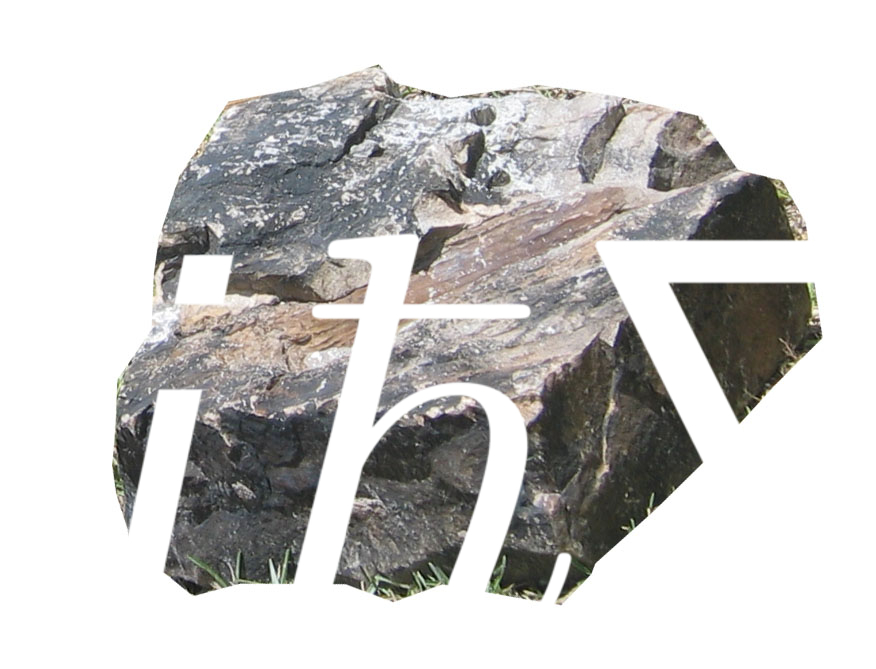
\includepdf{cover.pdf}
% nothing behind the cover...
\newpage\null\thispagestyle{empty}\newpage
% at the left we have the dedicatory, as expected.
\includepdf{dedicatory.pdf}

\setcounter{tocdepth}{1}
\tableofcontents


\part{Teoría}
\chapter{Rotaciones}
En este capítulo se contemplan las rotaciones en $\mathbb{R}^3$
\emph{activas} (que giran el sistema físico y no el marco de
referencia). Son transformaciones lineales $\boldrm{x} \to R\boldrm{x}$ que conservan la norma,
representadas por matrices $3 \times 3$ tales que $\det R = 1$.

Todas las rotaciones en ejes arbitrarios con origen fijo conforman el
\emph{grupo de rotación 3D}, también llamado $SO(3)$. Se puede
parametrizar con un eje de giro y un ángulo o con los tres ángulos de
Euler. $SO(3)$ es un \emph{grupo de Lie}, por lo que se puede ir de
una rotación a otra de manera continua.

Con el convenio de la ``mano derecha'' para los ángulos, podemos ver
las matrices correspondientes a rotaciones en los ejes principales:
\begin{align}
  R_{\text{OX}} &=
  \begin{pmatrix}
    1 & 0 & 0 \\
    0&\cos \theta & -\sin \theta  \\
    0&\sin \theta & \cos \theta  
  \end{pmatrix} \\
  R_{\text{OY}} &=
  \begin{pmatrix}
    \cos \theta &0& \sin \theta  \\
    0 & 1 & 0 \\
    -\sin \theta & 0&\cos \theta  \\
  \end{pmatrix} \\
  R_{\text{OZ}} &=
  \begin{pmatrix}
    \cos \theta & -\sin \theta & 0 \\
    \sin \theta & \cos \theta & 0 \\
    0 & 0 & 1 
  \end{pmatrix}
\end{align}

Investiguemos que ocurre si hacemos una rotación infinitesimal con
ángulo $\varepsilon$. Para ello, tomamos la matriz $R_\text{OZ}$ (más
tarde se extenderá el resultado) y aproximamos $\sin \varepsilon \sim
\varepsilon$ y $\cos \varepsilon \sim 1$:
\begin{equation}
  R_\text{OZ}(\varepsilon) \sim
  \begin{pmatrix}
    1 & -\varepsilon & 0 \\
    \varepsilon &  1 & 0 \\
    0 & 0& 1
  \end{pmatrix}
\end{equation}
La nueva matriz es prácticamente ortogonal, ya que la norma de sus
columnas es $1$ o $1 + \varepsilon^2 \sim 1$. Puede escribirse de forma
especial:
\begin{equation}
  R_\text{OZ}(\varepsilon) = \mathbb{I} - i \varepsilon
  \underbrace{
   \begin{pmatrix}
    0 & -i & 0 \\
    i & 0 & 0 \\
    0 & 0 & 0 
  \end{pmatrix}}_{G_z}
\end{equation}
donde $G_z$ (de ``generador'') es hermítica y ortogonal. Para los
demás ejes tenemos:
\begin{align}
  G_x &=
  \begin{pmatrix}
    0 & 0 & 0 \\
    0&0 & -i  \\
    0&i&0 
  \end{pmatrix} \\
  G_y &=
  \begin{pmatrix}
    0 & 0 & i \\
    0&0 & 0  \\
    -i&0&0 
  \end{pmatrix} \\
  G_z &=
  \begin{pmatrix}
    0 & -i & 0 \\
    i&0 & 0  \\
    0&0&0 
  \end{pmatrix}
\end{align}
Las matrices $G_i$ son los generadores infinitesimales
\index{generador infinitesimal}de rotaciones
en $\mathbb{R}^3$. Se puede ver que $[G_x,G_y]=iG_z$, o de forma
general:
\begin{equation}
  [G_i,G_j] = i\varepsilon_{ijk} G_k
\end{equation}
donde $\varepsilon_{ijk}$ es el \emph{símbolo de Levi-Civita}, evaluado
en $i,j,k = x,y,z$.

Con sumas de estas matrices se puede llegar a cualquier rotación.
Esta álgebra es una \emph{algebra de Lie}. Veamos que, en efecto, es
posible reconstruir una rotación. Rotamos un vector $\boldrm{x}$:
\begin{equation}
  \boldrm{x} \to (\mathbb{I}-i\varepsilon G_z)\boldrm{x} = R_z(\varepsilon)\boldrm{x}
\end{equation}
Como las rotaciones en el mismo eje conmutan entre sí, puedo escribir
\begin{equation}
  \begin{split}
    R_z(\theta+\varepsilon) &= R_z(\varepsilon)R(\theta) = [\mathbb{I} -
    i\varepsilon G_z] R_z(\theta) =\\
    &= R_z(\theta) - i\varepsilon G_z R_z(\theta)
  \end{split}
\end{equation}
Si suponemos $\varepsilon \to 0$ tenemos una ecuación diferencial formal
en $R_z(\theta)$:
\begin{align}
  \frac{R_z(\theta+\varepsilon) - R_z(\theta)}{\varepsilon} &= - i
  G_z R_z(\theta) \\
  \frac{\text{d}}{\text{d}\theta}R_z(\theta) &= -i G_z R_z(\theta)
\end{align}
Es una ecuación para operadores, de solución exponencial:
\begin{equation}
  R_z(\theta) = \exp(-i\theta G_z)\cdot \text{cte.}
\end{equation}
donde $\text{cte.} =1$ ya que $R_z(0) = \mathbb{I}$. Como $G_z$ es
hermítica, la suma exponencial converge sin problemas:
\begin{equation}
  \begin{split}
    e^{-i\theta G_z} &= \mathbb{I}-i \theta G_z -
    \frac{\theta^2}{2!}G_z^2 + i \frac{\theta^3}{3!} G_z^3 + \cdots =
    \\
    &= \mathbb{I} + G_z \left( -i\theta + i \frac{\theta^3}{3!} +
      \cdots \right) + G_z^2 \left( - \frac{\theta^2}{2!} +
      \frac{\theta^4}{4!} + \cdots \right) =\\
    &= \mathbb{I} - i \sin \theta G_z + (\cos\theta -1)G_z^2 = \\
    &= R_{\text{OZ}}
  \end{split}
\end{equation}
donde se ha usado que $G_z^3 = G_z$.

De forma general, para un eje cualquiera $\hat{n}$ se tiene
\begin{equation}
  R_{\hat{n}}(\theta) = e^{-i\theta \boldrm{G}\cdot \hat{n}}
\end{equation}
donde $\boldrm{G} = (G_x,G_y,G_z)$. Notar que $e^{-i\theta
  \boldrm{G}\cdot \hat{n}} $ es factorizable en producto de
exponenciales sólo si los operadores $G_i$ conmutan, y
no es el caso.

\section{Aplicaciones}
Con lo visto, podemos encontrar analíticamente las rotaciones en
diversos espacios vectoriales de la mecánica cuántica.
\subsection{Espacios de Hilbert $ \Ham $}
El espacio de las funciones de onda sin espín es un espacio de
Hilbert. Las rotaciones transforman a las funciones de onda $\varphi$ en
nuevas $\varphi'$. 

La intuición geométrica\index{intuición} nos dice que para una rotación de ángulo
definido la materia se ha movido de $\boldrm{x}$ a $\boldrm{x}'$, y la
función de ondas vale en todos los puntos el valor que había antes en
el ángulo recorrido en sentido contrario. De manera formal:
\begin{equation}
  \varphi'(\boldrm{x}') = \varphi(\boldrm{x}), \ \forall \boldrm{x}' \
  \rightarrow \ \varphi'(\boldrm{x}) = \varphi(R^{-1}\boldrm{x})
\end{equation}
El operador que desplaza a las $\boldrm{x}$ es $R$; nos preguntamos
cuales son las propiedades del endomorfismo $U$ que translada a las
funciones de onda $\varphi$. Damos por descontado\footnote{Cohen no. Ver
allí demostración rigurosa.} que es lineal y unitario. 
Su definición
viene dada de forma implícita por $\varphi'(\boldrm{x}) =
\varphi(R^{-1}\boldrm{x})$; veamos su forma en una rotación
infinitesimal. Comenzamos por calcular $R^{-1}(\varepsilon)$ para el eje
z (de nuevo, posteriormente se verá el caso general):
\begin{equation}
  R^{-1}_z(\varepsilon) \sim
  \begin{pmatrix}
    \cos \theta & \sin \theta & 0 \\
    -\sin \theta & \cos \theta & 0 \\
    0 & 0 & 1 
  \end{pmatrix}_{\theta \to \varepsilon \sim 0} =
  \begin{pmatrix}
    1 & \varepsilon & 0 \\
    -\varepsilon&1 & 0 \\
    0 & 0 & 1
  \end{pmatrix}
\end{equation}
Por tanto,
\begin{equation}
  \varphi'(x,y,z) = \varphi(R^{-1}_z(\varepsilon) \boldrm{x}) =
  \varphi(\boldrm{x}'), \ \ \boldrm{x}' =
  \begin{pmatrix}
    x+\varepsilon y \\
    y-\varepsilon x \\
    z
  \end{pmatrix}
\end{equation}
Como $\varepsilon$ es muy pequeño, efectuamos un desarrollo en serie
de potencias:
\begin{equation}
  \begin{split}
    \varphi'(\boldrm{x}) &= \varphi(\boldrm{x}) + \pdv{\varphi}{x}
    \underbrace{\Delta x}_{\varepsilon y} + \pdv{\varphi}{y}
    \underbrace{\Delta y}_{-\varepsilon x} + \pdv{\varphi}{z}
    \cancelto{0}{\Delta z} = \\
    &= \varphi(\boldrm{x}) - \varepsilon \left[ \pdv{\varphi}{y} x -
      \pdv{\varphi}{x}y \right] = \varphi(\boldrm{x})-\varepsilon i \frac{L_z}{\hbar}\varphi
  \end{split}
\end{equation}
donde $L_z$ es la componente $z$ del operador momento angular.
Concluimos por tanto que
\begin{equation}
  \boxed{
    \varphi'(\boldrm{x}) = \left( \mathbb{I}-i \varepsilon \frac{L_z}{\hbar} \right)\varphi(\boldrm{x})
  }
\end{equation}

Hemos obtenido que $L_z/\hbar = U$ es el generador
infinitesimal\index{generador infinitesimal} de
las rotaciones en el espacio de Hilbert de las funciones de onda sin
espín. De manera similar, en el eje $y$ el operador relevante es
$L_y/\hbar$ y $L_x/\hbar$ en el eje $x$. Tenemos una relación similar
a la de los $G_i$ con los operadores momento angular:
\begin{equation}
  \left[ \frac{L_i}{\hbar}, \frac{L_j}{\hbar} \right] = i
  \varepsilon_{ijk} \frac{L_k}{\hbar}
\end{equation}
Notar que mientras las $G_i$ son matrices, los $L_i$ son operadores
diferenciales. Esto se debe a que los espacios sobre los que actúan
son muy distintos ($\mathbb{R}^3$ y el espacio de Hilbert $ \Ham $).

Con argumentos similares a los usados para $\mathbb{R}^3$, definimos
una rotación finita en el eje $z$ como $U_z(\theta) = e^{-i\theta
  \frac{L_z}{\hbar}}$, y en un eje arbitrario $\hat{n}$ como
\begin{equation}
  U_{\hat{n}} (\theta)= \exp \left(  {-i \theta
      \frac{\boldrm{L}\cdot\hat{n}}{\hbar}} \right)
\end{equation}
Recordar que la exponencial no es factorizable por no conmutar los
$L_i$. En este caso no podemos calcular la exponencial del operador
como serie por no conocer la relación de recurrencia de sus potencias.

\subsection{Espacios complejos $\mathbb{C}^2$}
Los espines de los electrones ($\oh$) pertenecen a
$\mathbb{C}^2$, ya que para definir el espín en cada punto del espacio
son necesarios dos números complejos. Las funciones de onda de estas
partículas necesitan además una extensión a espacio de Hilbert:
\begin{equation}
  \begin{split}
    \varphi &= \binom{f(\boldrm{r})}{g(\boldrm{r})} = f(\boldrm{r})
    \otimes \binom{1}{0} + g(\boldrm{r}) \otimes \binom{0}{1} \\
    &=  f(\boldrm{r})
    \otimes \ket{+} \  + \  g(\boldrm{r}) \otimes \ket{-} \in
     \Ham \otimes \mathbb{C}^2
  \end{split}
\end{equation}
A los \emph{ket} $\ket{+},\ket{-}$ se les suele llamar \emph{espinores}.
Para que $\varphi$ sea de cuadrado integrable, las funciones $f,g$ han de
cumplir que la integral de sus módulos al cuadrado sobre todo el
espacio valgan la unidad.

De manera inocente podría pensarse en que una rotación puede
escribirse como
\begin{equation}
  \binom{f'(\boldrm{r})}{g'(\boldrm{r})} = \binom{f(R^{-1}\boldrm{r})}{g(R^{-1}\boldrm{r})}
\end{equation}
pero no es así, los vectores se transforman de forma más complicada
que los escalares. Necesitamos utilizar los generadores de
$\mathbb{C}^2$, las \emph{matrices de Pauli}:
\begin{equation}
  S_x = \frac{\hbar}{2} \begin{pmatrix} 0 & 1 \\ 1 & 0 \end{pmatrix};  \ \ 
  S_y = \frac{\hbar}{2} \begin{pmatrix} 0 & -i \\ i & 0 \end{pmatrix};  \ \ 
  S_z = \frac{\hbar}{2} \begin{pmatrix} 1 & 0 \\ 0 & -1 \end{pmatrix}
\end{equation}
Las rotaciones en un eje arbitrario vendrán dadas por
\begin{equation}
  R_{\hat{n}}(\theta) = \exp \left( -i \theta
    \frac{\boldrm{S}\cdot\hat{n}}{\hbar} \right) \in \mathbb{C}^2
\end{equation}
Resolviendo la serie de potencias se obtiene
\begin{equation}
  R_{\hat{n}}(\theta) = \mathbb{I}\cos \frac{\theta}{2} - i
  (\boldrm{\sigma}\cdot \hat{n}) \sin \frac{\theta}{2}
\end{equation}
donde $\boldrm{\sigma} = \frac{2}{\hbar}\boldrm{S}$. Un espinor $\chi$
``apunta'' en la dirección $\hat{n}$ si
$(\boldrm{\sigma}\cdot\hat{n})\chi = +1 \chi$

Puede comprobarse que, por ejemplo, un giro en $z$ no varía el valor
del espín en $z$. No obstante, aunque podría esperarse que el operador
$R_{\hat{n}}(2\pi) = \mathbb{I}$, resulta que lo que se obtiene es
$-\mathbb{I}$. Notar que esto es irrelevante, ya que lo que se mide es
siempre $\bra{\varphi|A}\ket{\varphi}$ o $|\varphi|^2$, que son siempre positivos.

\subsection{Espacios de partículas con espín $ \Ham \otimes \mathbb{C}^2$}
Resueltos los giros en $\mathbb{C}^2$ y en los espacios de Hilbert, ya
solo queda extender los resultados al producto de ambos espacios. Como
es razonable pensar, basta con girar primero la órbita y luego el
espín. De manera formal, el efecto del operador $U$ sobre el espinor
con función de onda $\varphi(\boldrm{r})\otimes \chi$ es:
\begin{equation}
  \left( e^{-i\theta \frac{1}{\hbar}\boldrm{L}\hat{n}} \otimes
    e^{-i\theta \frac{1}{\hbar}\boldrm{S}\hat{n}}\right)
  [\varphi(\boldrm{r})\otimes \chi] = \left( e^{-i\theta
      \frac{1}{\hbar}\boldrm{L}\hat{n}}\varphi(\boldrm{r}) \right)
  \otimes \left( e^{-i\theta \frac{1}{\hbar}\boldrm{S}\hat{n}}\chi \right)
\end{equation}
Realicemos una rotación infinitesimal, para ver la forma de los
generadores. Utilizamos $\hat{n}=z$; sea $\theta \to \varepsilon\sim 0$:
\begin{equation}
  \begin{split}
  U [\varphi(\boldrm{r})\otimes \chi] &= \left( e^{-i\theta
      \frac{1}{\hbar}\boldrm{L}\hat{n}}\varphi(\boldrm{r}) \right)
  \otimes \left( e^{-i\theta \frac{1}{\hbar}\boldrm{S}\hat{n}}\chi
  \right)= \\
  &= \left( \mathbb{I}-i\varepsilon \frac{L_z}{\hbar} \right)\varphi \otimes
  \left( \mathbb{I}-i\varepsilon \frac{S_z}{\hbar} \right) \chi = \\
  &= \varphi\otimes \chi - i\varepsilon \left( \frac{L_z}{\hbar}\varphi \right)\otimes \chi  - i \varepsilon
  \left( \frac{S_z}{\hbar}\chi \right)\otimes \varphi  +
  \order{\varepsilon^2} \cdots
  \end{split}
\end{equation}

Los operadores del segundo y tercer sumando se pueden reescribir como
extensiones al espacio producto vectorial; para el momento angular
tenemos $L_z \varphi \otimes \chi = (L_z\otimes \mathbb{I})[\varphi \otimes
\chi]$ y para la matriz de Pauli $ \varphi \otimes S_z\chi = ( \mathbb{I} \otimes
S_z)[\varphi \otimes \chi]$. Con ello, obtenemos
\begin{equation}
  =\varphi \otimes \chi - i \frac{\varepsilon}{\hbar} (L_z\otimes \mathbb{I}+
  \mathbb{I}\otimes S_z)
  [\varphi\otimes\chi] + \order{\varepsilon^2} = \cdots
\end{equation}
que con un una notación más laxa\footnote{No hay que dejar que esta
  notación nos haga olvidar que dos operadores de espacios vectoriales
distintos no se pueden sumar como si tal cosa. Por ejemplo, $S_{1z}+S_{2z}$
no es $\frac{\hbar}{2}\begin{pmatrix} 1 & 0 \\ 0 & -1 \end{pmatrix} +
\frac{\hbar}{2}\begin{pmatrix} 1 & 0 \\ 0 & -1 \end{pmatrix}  =
\hbar \begin{pmatrix} 1 & 0 \\ 0 & -1 \end{pmatrix} $, sino la matriz
$4\times 4$ que corresponde a $S_{1z}\otimes \mathbb{I} +
\mathbb{I}\otimes S_{2z} = \begin{pmatrix} (S_{1z}) & 0 \\ 0 & (S_{2z}) \end{pmatrix}$ } podemos escribir como
\begin{equation}
  =\varphi \otimes \chi - i \frac{\varepsilon}{\hbar} (L_z+
  S_z)
  [\varphi\otimes\chi] + \order{\varepsilon^2} = \cdots
\end{equation}
Teniendo en cuenta que $L_z + S_z = J_z$ (operador \emph{momento
  angular total}), obtenemos
\begin{equation}
  \cdots = \left( \mathbb{I} - i \varepsilon \frac{J_z}{\hbar}
  \right)[\varphi\otimes \chi]
\end{equation} 
Obtenemos que el momento angular total es el generador de las
rotaciones en el espacio $ \Ham \otimes \mathbb{C}^2$. En
un espacio general se utiliza $\boldrm{J}_T = \sum_{ }\boldrm{J}_i +
\sum_{ }\boldrm{S}_i$. Notar de nuevo que $\boldrm{J}$ y $\boldrm{S}$
pertenecen a espacios distintos y no son sumables; en realidad nos
referimos a sus extensiones a $ \Ham \otimes \mathbb{C}^2$. Las
rotaciones en un eje arbitrario vendrán dadas por
\begin{equation}
R_{\hat{n}} (\theta) = \exp \left( -i \varepsilon \frac{\boldrm{J}_T\cdot
    \hat{n}}{\hbar} \right) = e^{-i\theta \frac{\boldrm{L}_1 \cdot
    \hat{n}}{\hbar}} e^{-i\theta \frac{\boldrm{S}_1 \cdot \hat{n}}{\hbar}}
\cdots e^{-i\theta \frac{\boldrm{L}_N \cdot \hat{n}}{\hbar}} e^{-i\theta \frac{\boldrm{S}_N \cdot \hat{n}}{\hbar}}
\end{equation}
donde $N$ es el número de partículas del sistema. Cada operador actúa
sobre sus funciones de onda correspondientes, recordar que en esta
notación faltan muchas extensiones (varios factores ``$\otimes \mathbb{I}$'' ).

\section{Rotación de observables}
Imaginemos un montaje experimental como el de Stern-Gerlach; hacemos
pasar electrones (espín $\oh$) por un campo magnetico
$\boldrm{B}\propto \hat{z}$
fuerte y vemos como el haz se divide en dos, colisionando con una
pantalla fluorescente. Estamos midiendo el
autovalor del observable $S_z$, y se obtienen de manera equiprobable
los valores $\pm \nicefrac{\hbar}{2}$. Si polarizamos los espines
sólo se obtendrá una mancha, por ejemplo la del autovalor $\nicefrac{\hbar}{2}$.

Si rotamos todo el sistema de forma que el campo magnético esté
orientado ahora en $\hat{x}$ estaremos midiendo el observable $S_x$,
pero seguiremos obteniendo el autovalor $\nicefrac{\hbar}{2}$ (la
mancha seguirá en el mismo sitio de la pantalla).

Deducimos por tanto que rotar un sistema
físico\jokenote{Es nuestro hecho diferencial el no
girar el sistema de coordenadas. Nos hace diferentes, es
decir, nos hace mucho mejores que los demás.} cambia el
obserbable
pero no el autovalor. Sea un observable $A$ de autovalores $a_n$ y
autovectores $u_n$, si efectuamos una rotación en el espacio de
Hilbert $u_n \to Ru_n = u_n'$ obtenemos
\begin{equation}
  A u_n = a_n u_n \ \stackrel{R}{\rightarrow} \ A'u_n' = a_n u_n'
\end{equation}
Nos preguntamos la relación entre el nuevo operador y el original.
Para averiguarlo, utilizamos que $u' = Ru$:
\begin{equation}
  \begin{split}
    A' u'_n &= a_n u_n' \\
    A' Ru_n &= a_n Ru_n \\
    A' Ru_n &= R a_n u_n \\
    R^{-1}A' Ru_n &=  a_n u_n  \\
    R^{-1}A' Ru_n &=  A u_n  \\
  \end{split}
\end{equation}
Por lo tanto
\begin{equation}
  \boxed{A' = R A R^\dagger}
\end{equation}
donde se ha utilizado que para matrices hermíticas $R^{-1}MR=RMR^\dagger$.

\subsection{Observables escalares e invariancia bajo rotaciones}
Un ejemplo es $\boldrm{S}^2 = \frac{3}{4} \hbar \mathbb{I}$.
Supongamos ahora que $R$ es infinitesimal; en tal caso:
\begin{equation}
  R = \left( \mathbb{I} - \frac{i\varepsilon}{\hbar}\boldrm{J}\cdot\hat{n} \right)
\end{equation}
y por lo tanto
\begin{equation}
  \begin{split}
    A' &= \left( \mathbb{I} - \frac{i\varepsilon}{\hbar} \boldrm{J}\cdot
      \hat{n} \right) A \left( \mathbb{I} + \frac{i\varepsilon}{\hbar}
      \boldrm{J}\cdot \hat{n} \right) = \\
    &= A - \frac{i\varepsilon}{\hbar}(\boldrm{J}\cdot\hat{n})A + A
    \frac{i\varepsilon}{\hbar}(\boldrm{J}\cdot\hat{n}) +
    \order{\varepsilon^2} = \\
    &= A - \frac{i\varepsilon}{\hbar} [\boldrm{J}\hat{n},A]
  \end{split}
\end{equation}
Si $A$ conmuta con cualquier función de $J$ se obtiene $A'= A$. Esta
relación de conmutación con $\boldrm{J}$ es muy relevante cuando $A$
es el hamiltoniano, se le denota \emph{invariancia bajo rotaciones}.

Cuando un sistema es invariante bajo rotaciones para un observable es
señal de que este es escalar, evitando romperse la simetría cuando
rotamos el sistema. 

Imaginemos una partícula libre en el plano, si rotamos el sistema un
ángulo $\theta$ el movimiento seguirá siendo el mismo salvo por la
rotación. Si en cambio rotamos un sistema con una fuerza vectorial,
como un tiro parabólico en un campo gravitatorio, la trayectoria ya no
será la misma aunque rotemos las condiciones iniciales; habría que
rotar también la fuerza externa.

De manera formal, en los sistemas con invariancia entre rotaciones
esperamos la siguiente regla de transformación:
\begin{equation*}
  \begin{matrix}
    \psi(t_0) & \stackrel{ \Ham }{\rightarrow} & \psi(t) \\
    \downarrow R & & \downarrow R \\
    \psi'(t_0) & \stackrel{ \Ham }{\rightarrow} & \psi'(t)
  \end{matrix}
\end{equation*}
Notar que los dos operadores $R$ son el mismo.

Si hay invariancia ante rotaciones, utilizando la ecuación de
Schrödinger ($i \hbar \dot{\psi} =  \Ham \psi$) es esperable que
\begin{equation}
  \begin{split}
    \psi'(t_0 + \dd{t}) &= \psi'(t_0) - \frac{i}{\hbar} \dd{t}
     \Ham  \psi'(t_0) \\
    \psi(t_0 + \dd{t}) &= \psi(t_0) - \frac{i}{\hbar} \dd{t}  \Ham  \psi(t_0)
  \end{split}
\end{equation}
como $\psi'(t_0 + \dd{t}) = R \psi(t_0 + \dd{t})$, sustituyendo
obtenemos
\begin{equation}
  \psi'(t_0)-\frac{i}{\hbar}\dd{t} \Ham \psi'(t_0) = R \psi (t_0)
  - \frac{i}{\hbar}\dd{t}R  \Ham  \psi(t_0)
\end{equation}
y utilizando que $\psi'(t_0) = R \psi(t_0)$ obtenemos que
\begin{equation}
   \Ham R\psi = R  \Ham  \psi, \ \forall \psi,t_0,R
\end{equation}
Por lo tanto $[ \Ham ,R] = 0$. Hemos obtenido que el hamiltoniano
es un operador escalar bajo rotaciones. De igual forma conmuta con
$\boldrm{J}$ y $\boldrm{L}$. Una consecuencia inmediata es que sus
autovalores están degenerados; a esta degeneración se le denota
\emph{degeneración natural}. 

\begin{proof}[Degeneración de la energía]
  Sean $E$ y $\ket{\alpha,j,m}$ un autovalor y autovector del
  hamiltoniano. Aplicamos en la ecuación de Schrödinger independiente
  del tiempo un operador escalera al autovector:
  \begin{equation}
     \Ham  J_\pm \ket{\alpha,j,m} = \sqrt{j(j+1) - m(m\pm 1)}
    \hbar  \Ham  \ket{\alpha,j,m\pm1}
  \end{equation}
  Como $ \Ham $ conmuta con $\boldrm{J}$, también conmuta con
  cualquier combinación lineal de sus componentes. Como los operadores
  escalera se construyen como combinación lineal de los componentes de
  $\boldrm{J}$, el hamiltoniano conmuta con $J_\pm$ y podemos escribir
  que $ \Ham J_\pm = J_\pm  \Ham $. Por tanto,
  \begin{equation}
    \begin{split}
      J_\pm \Ham  \ket{\alpha,j,m} &= J_\pm E \ket{\alpha,j,m} =
      \\ &= E
      \sqrt{j(j+1) - m(m\pm 1)} \hbar \ket{\alpha,j,m\pm1} = \\
      &= \sqrt{j(j+1) - m(m\pm 1)}
    \hbar  \Ham  \ket{\alpha,j,m\pm1} =\\ &=  \Ham J_\pm \ket{\alpha,j,m}
    \end{split}
  \end{equation}
  obtenemos que $ \Ham \ket{\alpha,j,m\pm1} = E
  \ket{\alpha,j,m\pm1}$. Por tanto hay degeneración para una energía
  $E$ fija, como mínimo $2j+1$ (número de estados $m$).
\end{proof}

\subsection{Ejemplo: potenciales centrales}
Sea una partícula de masa $m$ en un potencial central $V(r)$. El
hamiltoniano\jokenote{Y os preguntaréis, ¿por qué
quiero medir eso? Pues porque sois físicos, no filósofos. Si
no queréis medir nada os vais a la facultad de enfrente, que
os acogerán con los brazos abiertos porque les faltan
alumnos.} es:
\begin{equation}
   \Ham  = \frac{-\hbar^2}{2m}\nabla^2 + V(r)
\end{equation}
Claramente conmuta con rotaciones respecto al centro de fuerzas por
simetría. Tenemos que $[ \Ham ,\boldrm{L}] = 0$, y por tanto
$ \Ham ,L^2,L_z$ comparten autovalores.

La simetría del problema nos permite escribir el hamiltoniano de
forma puramente radial, encerrando la dependencia angular en $\boldrm{L}^2$:
\begin{equation}
   \Ham  = \frac{-\hbar^2}{2m} \left[ \frac{1}{r^2} \pdv{}{r}
    \left( r^2 \pdv{}{r} \right) - \frac{\boldrm{L}^2}{\hbar^2 r^2} \right] + V(r)
\end{equation}
Podemos expresar sus soluciones como producto de una parte radial y
otra angular:
\begin{equation}
  \psi = R(r) Y_\ell^m(\theta,\varphi)
\end{equation}
Si sustituyo $\psi$ en la ecuación de Schrödinger independiente del
tiempo, se pueden cancelar de ambos lados de la ecuación los armónicos
esféricos, y se obtiene:
\begin{equation}
  \frac{-\hbar^2}{2m} \dv[2]{}{r} \chi_\ell(r) + \underbrace{\left[ V(r) +
    \frac{\hbar^2}{2mr^2} \ell (\ell+1) \right]}_{V_\text{eff}} \chi_\ell(r) = E \chi_\ell(r)
\end{equation}
donde hay una solución para cada $\ell$, por lo que hay que indexar las
$\chi$. Por último, imponemos condiciones de contorno:
\begin{equation}
  \int_{0}^\infty |R(r)|^2 r^2 \dd{r} = \int_{4\pi}
  |Y_\ell^m(\theta,\varphi)|^2 \dd{\Omega} = 1
\end{equation}
Si nos dan un autovalor podemos conocer el autoestado correspondiente,
que está degenerado con los estados de igual energía:
\begin{equation}
  R_\ell(r)Y_\ell^m(\theta,\varphi), \ m = 2\ell+1
\end{equation}
Notar que aunque es una ecuación de segundo orden sólo se ha hablado
de una de las soluciones. Esto es debido a que la otra no es
normalizable por poseer una divergencia en $r=0$.

%%% Local Variables:
%%% mode: latex
%%% TeX-master: "../resumen"
%%% End:

\chapter{Métodos perturbativos}
Comenzamos el estudio de los métodos perturbativos por las
perturbaciones estacionarias. En ellas tenemos fuerzas no dependientes
del tiempo actuando sobre el sistema.

Escribimos el hamiltoniano del sistema como la suma de un hamiltoniano
sin perturbar $ \Ham _0$ y una perturbación $W$ despreciable:
\begin{equation}
   \Ham  =  \Ham _0 + W 
\end{equation}
No estamos comparando energías, sino operadores, lo que dificulta
identificar cuando $W$ es realmente despreciable.

Suponemos que para $ \Ham _0$ conocemos la solución a la ecuación de
autovalores:
\begin{equation}
   \Ham _0 \ket{\varphi_p^i} = E_p \ket{\varphi_p^i}
\label{eq:originalH}
\end{equation}
donde $p$ es el índice que indexa los distintos autovectores y $i$ el
índice para diferenciar soluciones en caso de existir degeneración.
Utilizaremos los $\ket{\varphi_p^i}$ como base del espacio.

Escribimos $W=\lambda \hat{W}$ de forma que podamos ``regular'' el
efecto de la perturbación con el factor escalar $\lambda$, con lo que
obtenemos $ \Ham (\lambda) =  \Ham _0 + \lambda\hat{W} $.
Nos queda
\begin{equation}
   \Ham  \varphi(\lambda) = E(\lambda)\varphi(\lambda)
\label{eq:lambdaschr}
\end{equation}
Tratamos de hallar la $E(\lambda)$. Si la perturbación no es muy
grande, es de suponer que $\{E(\lambda)\} \sim \{E_p\}$. 

Utilizando series de potencias:
\begin{align}
  E(\lambda) &= \varepsilon_0 + \varepsilon_1 \lambda + \varepsilon_2 \lambda^2
  + \cdots \\
  \varphi(\lambda) &= \ket{0} + \lambda \ket{1} + \lambda^2 \ket{2} 
  + \cdots 
                  \label{eq:varphilamb}
\end{align}
Escribimos la ecuación de Schrödinger \eqref{eq:lambdaschr}:
\begin{equation}
  ( \Ham _0 + \lambda \hat{W})[\ket{0} + \lambda \ket{1} +
  \cdots] = \left( \sum_{i=1}^\infty \varepsilon_i \lambda^i  \right)
  \left( \sum_{i=1}^\infty \lambda^i \ket{i}  \right)
\end{equation}
Igualamos las distintas potencias de $\lambda$:
\begin{equation}
  \begin{split}
    \lambda^0 &:\ \  \Ham _0 \ket{0} = \varepsilon_0 \ket{0} \\
    \lambda^1 &:\ \  \Ham _0 \ket{1} + \hat{W} \ket{0} =
    \varepsilon_0 \ket{1}+ \varepsilon_1 \ket{0} \\
    \lambda^2 &:\ \  \Ham _0 \ket{2} + \hat{W} \ket{1} =
    \varepsilon_0 \ket{2} +\varepsilon_1 \ket{1} + \varepsilon_2 \ket{0} \\
    \cdots & \\
    \lambda^q &:\ \  \Ham _0 \ket{q} + \hat{W} \ket{q-1} =
    \varepsilon_0 \ket{q}+ \varepsilon_1 \ket{q-1} + \cdots + \varepsilon_q \ket{0} \\
  \end{split}
\end{equation}
A partir de orden 1 (lineal) se suele cortar la aproximación, ya que
no merece la pena precisar más por ser probablemente los $E_p$ usados
fruto de una aproximación.

Sabemos que \eqref{eq:lambdaschr} determina $\varphi(\lambda)$ sólo salvo
un factor de fase, lo que nos permite elegir la norma de
$\varphi(\lambda)$ y su fase. Escogemos que $\varphi(\lambda)$ esté
normalizado y tenga una fase tal que $\braket{0}{\varphi} \in
\mathbb{R}$. Utilizando esto en la ecuación \eqref{eq:varphilamb} surgen
varias consecuencias:
\begin{itemize}
\item En orden de aproximación nulo\footnote{ Si $\varphi(\lambda) \sim
    \ket{0}$ se obtiene
    \begin{equation*}
      \abs{\varphi(\lambda)}^2 = \braket{0}{0} = 1
    \end{equation*}
}, el ket $\ket{0}$ ha de estar
  normalizado.
\begin{equation}
  \braket{0}{0} =1
\end{equation}
\item A primer orden\footnote{Ahora $\varphi(\lambda)\sim \ket{0} +
    \lambda \ket{1}$ y se obtiene
    \begin{equation*}
      \begin{split}
        \abs{\varphi(\lambda)}^2 &= (\bra{0} + \lambda\bra{1})(\ket{0} +
        \lambda\ket{1}) = \\
        &= \cancelto{1}{\ip{0}} + \lambda\braket{0}{1} + \\ &+ \lambda\braket{1}{0} +
        \order{\lambda^2} = \\
        &= \cancel{1}
      \end{split}
    \end{equation*}
    Por lo que $\braket{0}{1}$ ha de ser igual a $-\braket{1}{0}$ y
    por tanto deben ser nulos.
    }, vemos que los kets $\ket{0}$ y $\ket{1}$ son
  perpendiculares:
\begin{equation}
  \braket{0}{1} = \braket{1}{0} = 0
\end{equation}
\item En segundo orden\footnote{
Las ecuaciones se complican, pero descartando términos
$\order{\lambda^3}$ y superiores se obtiene
\begin{equation*}
  \begin{split}
    \abs{\varphi(\lambda)}^2 
    &= \cancelto{1}{\ip{0}} + \cancelto{0}{\lambda\braket{0}{1}} + \lambda^2 \braket{0}{2} + \\
    &+  \cancelto{0}{\lambda\braket{1}{0}} + \lambda^2 \braket{1}{1} +
    \lambda^2 \braket{2}{0} = \\ &= \cancel{1}
  \end{split}
\end{equation*}
 Obtenemos que $\braket{2}{0} + \braket{0}{2} = -\braket{1}{1}$, y
 utilizando el convenio $\braket{2}{0} = \braket{0}{2}$ para las fases
 (puramente reales) se obtiene la ecuación \eqref{eq:captainamerica}.
},
\begin{equation}
  \braket{0}{2} = \braket{2}{0} = - \frac{1}{2} \braket{1}{1}
  \label{eq:captainamerica}
\end{equation}
\item En general, para orden $q$,
\begin{equation}
  \braket{0}{q} = - \frac{1}{2}\big[ \braket{q-1}{1} +
    \braket{q-2}{2} + \cdots + \braket{2}{q-2} + \braket{1}{q-1}\big]
\end{equation}
\end{itemize}

\section{Caso no degenerado}

\subsection{Orden 0}
Tomemos $ \Ham _0 \ket{0} = \varepsilon_0 \ket{0}$, que no es más que la
ecuación de autovalores de $ \Ham _0$ original
\eqref{eq:originalH}. Tenemos que, por tanto, $\varepsilon_0$ será alguno
de los $E_p$ y $\ket{0}$ alguno de los $\ket{\varphi_p^i}$. Como estamos
en el caso no degenerado nos olvidamos de los índices $i$, y tenemos
que para cada energía $\varepsilon_0 = E_p = E$ estamos ante $\ket{0} =
\ket{\varphi_p}$. En los sucesivos órdenes de aproximación refinaremos
este autoestado.

\subsection{Orden 1}
Ahora la ecuación a resolver es $ \Ham _0 \ket{1} + \hat{W}
\ket{0} = \varepsilon_0 \ket{1} + \varepsilon_1 \ket{0} $. Las incógnitas son
$\ket{1}$ y $\varepsilon_1$, ya que los términos cero se resolvieron en el
paso anterior.

Resolvemos la ecuación vectorial proyectando sobre un ket de la base de los $\ket{\varphi_p^i}$:

\begin{equation}
  \begin{split}
    \bra{\varphi_p}  \Ham _0 \ket{1} + \bra{\varphi_p} \hat{W} \ket{0}
    = \bra{\varphi_p} \varepsilon_0 \ket{1} + \bra{\varphi_p} \varepsilon_1 \ket{0} 
  \end{split}
\end{equation}
Como $ \Ham _0$ es hermítico puedo sacarlo del braket y escribir
$ \bra{\varphi_p} \Ham _0 = E_p \bra{\varphi_p}$. Reconociendo $\ket{0}
= \ket{\varphi_p}$:
\begin{equation}
  E_p \braket{\varphi_p}{1} + \bra{\varphi_p} \hat{W} \ket{\varphi_p} = E_p
  \braket{\varphi_p}{1} + \varepsilon_1 \cancelto{1}{\braket{\varphi_p}{\varphi_p}}
\end{equation}
Luego
\begin{equation}
  \boxed{
  \varepsilon_1 = \bra{\varphi_p} \hat{W} \ket{\varphi_p}}
\end{equation}
Truncando aquí, se obtiene que
\begin{equation}
  E(\lambda) = E_p +  \lambda \bra{\varphi_p} \hat{W} \ket{\varphi_p} + \order{\lambda^2}
\end{equation}
La corrección a la energía es simplemente el valor esperado del
operador $W = \lambda \hat{W}$.
No hemos explotado por completo la ecuación para $\lambda^1$, ya que
sólo hemos utilizado un ket de la base. Para obtener el ket $\ket{1}$
utilizamos el resto de elementos de la base $\varphi_{n\neq p}$:
\begin{equation}
  \begin{split}
    \bra{\varphi_n}  \Ham _0 \ket{1} + \bra{\varphi_n} \hat{W} \ket{0}
    &= \bra{\varphi_n} \varepsilon_0 \ket{1} + \bra{\varphi_n}
    \varepsilon_1 \ket{0} \\
    E_{n}\braket{\varphi_n}{1} + \bra{\varphi_n} \hat{W} \ket{0}
    &= \varepsilon_0 \braket{\varphi_n}{1} + \varepsilon_1
    \cancelto{0 }{\braket{\varphi_n}{0}} \\
    \left(  E_{n} - \varepsilon_0 \right) \braket{\varphi_n}{1}     &=  -  \bra{\varphi_n} \hat{W} \ket{0}
  \end{split}
\end{equation}
donde se ha utilizado que la base de autoestados es ortogonal, y por
tanto $\braket{\varphi_n}{0} = \braket{\varphi_n}{\varphi_p} = 0$.
Obtenemos:
\begin{equation}
     \braket{\varphi_n}{1}=    \frac{-\bra{\varphi_n} \hat{W} \ket{0}}{
       E_n-\varepsilon_0}\ \ \ (p \neq n)
\end{equation}
Ahora conocemos la expansión del ket $\ket{1}$ en la base conocida de
los $\ket{\varphi_p^i}$, salvo el coeficiente correspondiente a $p = n$.
Pero ese coeficiente es $\braket{\varphi_p}{1} = \braket{0}{1} = 0$. De
manera explícita:
\begin{equation}
  \boxed{
 \ket{1} = \sum_{n\neq p} \sum_{i}
 \frac{\bra{\varphi_n^i}\hat{W}\ket{0}}{\varepsilon_0 - E_n} \ket{\varphi_n^i}
 \label{eq:ket1}}
\end{equation}
y por tanto, hasta orden 1, el autoestado del hamiltoniano
correspondiente al estado sin perturbación $\varphi_p$ puede escribirse como
\begin{equation}
 \varphi(\lambda) = \underbrace{\ket{0}}_{\varphi_p} +\lambda  \sum_{n\neq p} \sum_{i}
 \frac{\bra{\varphi_n^i}\hat{W}\ket{0}}{\varepsilon_0 - E_n} \ket{\varphi_n^i}
 + \order{\lambda^2}
\end{equation}
La corrección del autoestado es una combinación lineal de los demás
autoestados. Notar que hay términos que pesan más que otros en el
sumatorio. En general, cuanto más próximas al nivel en perturbación
sean las energías de los estados, y cuanto más grande sea el
acoplamiento producido por el elemento de matriz de $W$, mayor será el
peso de ese autoestado en la corrección. 

\subsection{Orden 2}
Utilizamos la ecuación para $\lambda^2$:
\begin{equation}
   \Ham _0 \ket{2} + \hat{W} \ket{1} = \varepsilon_0 \ket{2} +
  \varepsilon_1 \ket{1}  + \varepsilon_2 \ket{0}
\end{equation}
Proyectamos sobre un $\bra{\varphi_p}$ y volvemos a utilizar que $
\bra{\varphi_p}  \Ham _0 \ket{2} = E_p \braket{\varphi_p}{2}$. Como
además $\ket{0}\perp\ket{1}$,
\begin{equation}
 \cancel{ E_p \braket{\varphi_p}{2}} + \bra{\varphi_p}\hat{W}\ket{1} = \cancel{\varepsilon_0
  \braket{\varphi_p}{2}} + \varepsilon_1 \braket{\varphi_p}{1} +
\varepsilon_2\braket{\varphi_p}{0} 
\end{equation}

Como $\ket{\varphi_p} = \ket{0}$, tenemos
\begin{equation}
    \bra{\varphi_p}\hat{W}\ket{1} = \varepsilon_1 \cancelto{0}{\braket{0}{1}} +
    \varepsilon_2 \cancelto{1}{\braket{0}{0}}= \varepsilon_2
\end{equation}
Utilizando que $a \cdot a^\dagger = |a|^2$ y nuestro resultado de
\eqref{eq:ket1} para el ket $\ket{1}$,
\begin{equation}
  \begin{split}
    \varepsilon_2 &= \sum_{n\neq p} \sum_{i}
    \frac{\bra{\varphi_n^i}\hat{W}\ket{0}}{\varepsilon_0 - E_n}
    \bra{\varphi_p}\hat{W}|\varphi_n^i\rangle = \\ &= \sum_{n\neq p} \sum_{i}
    \frac{\bra{\varphi_n^i}\hat{W}\ket{0}}{\varepsilon_0 - E_n}
    \bra{0}\hat{W}|\varphi_n^i\rangle= \\ &= \sum_{n\neq p} \sum_{i}
    \frac{|\bra{\varphi_n^i}\hat{W}\ket{0}|^2}{\varepsilon_0 - E_n}
  \end{split}
\end{equation}
Como ya hemos hallado $\ket{1}$ en el orden anterior, ya tenemos
$\varepsilon_2$. Esto es un patrón común; aproximamos los autoestados
hasta orden $n$ pero la energía hasta orden $n+1$, aprovechando que
cuesta poco avanzar un orden en la energía pero no tan poco en los autoestados.

Muchas veces no hace falta calcular ese sumatorio, ya que es acotable:
\begin{equation}
  |\varepsilon_2| \leq \left|  \sum_{n\neq p} \sum_{i}
    \frac{|\bra{\varphi_n^i}\hat{W}\ket{0}|^2}{\varepsilon_0 - E_n} \right|
  \leq \frac{1}{\Delta E} \sum_{n\neq p} \sum_{i}
    |\langle\varphi_n^i|\hat{W}\ket{0^{}}|^2 = \cdots
\end{equation}
donde $\Delta E \leq |E_n - \varepsilon_0|$ es la menor de las
diferencias de energía.
  Dados unos $\ket{\varphi_n}$, el teorema del cierre afirma que $\sum_n
  \ket{\varphi_n}\bra{\varphi_n} = \mathbb{I}$. Como nuestros sumatorios son
  con $n \neq p$, incluimos el término \emph{ad hoc} y escribimos
  \begin{equation}
    \sum_{n \neq p} \ket{\varphi_n} \bra{\varphi_n} = \mathbb{I} - \ket{\varphi_p}\bra{\varphi_p}
  \end{equation}

  Obtenemos:
  \begin{equation}
    \begin{split}
      \cdots &=\frac{1}{\Delta E} \sum_{n \neq p} \sum_{i}
      |\langle\varphi_n^i|\hat{W}|0\rangle|^2 = \frac{1}{\Delta E} \sum_{n \neq p} \sum_{i}
      \langle 0|\hat{W}|\varphi_n^i\rangle \langle\varphi_n^i|\hat{W}|0\rangle  = \\ &=
      \frac{1}{\Delta E} \bra{0} \ \left[ \hat{W}
        (\mathbb{I}-\ket{0}\bra{0})\hat{W} \right]\  \ket{0} = \cdots
    \end{split}
  \end{equation}
  Identificando $\ket{0} = \ket{\varphi_p}$ escribimos
  \begin{equation}
    \cdots = \frac{1}{\Delta E} \left( \bra{\varphi_p}\hat{W}^2\ket{\varphi_p} -
      |\bra{\varphi_p}\hat{W}\ket{\varphi_p}|^2 \right) = \frac{(\Delta
      \hat{W})^2}{\Delta E}
  \end{equation}
  Por lo tanto
  \begin{equation}
    \boxed{
    |\lambda^2 \varepsilon_2| \leq \frac{1}{\Delta E}(\Delta W)^2}
  \end{equation}
  notar que hemos utilizado $W=\lambda\hat{W}$.


\section{Caso degenerado}
En orden $\lambda^0$ tenemos $ \Ham _0 \ket{0} = \varepsilon_0
\ket{0}$. Con o sin degeneración podemos identificar $\varepsilon_0 =
E_p$. Si no hay degeneración escribíamos $\ket{0} = \varphi_p$, pero
ahora sólo podemos afirmar que el ket $\ket{0}$ será una combinación
lineal del subespacio de degeneración de las $\ket{\varphi_p^i}$. Para
degeneración doble:
\begin{equation}
\ket{0} = a_1 \ket{\varphi_p^1} + a_2 \ket{\varphi_p^2} 
\label{eq:zerodegexp}
\end{equation}
Hay tantos sumandos como degeneración. La condición de normalización
en $\ket{0}$ nos da una primera ecuación:
\begin{equation}
  1 = |a_1|^2 + |a_2|^2
  \label{eq:zeronorm}
\end{equation}
Utilizando la ecuación en $\lambda^1$ ( $ \Ham _0 \ket{1} + \hat{W} \ket{0} = \varepsilon_0 \ket{1} +
  \varepsilon_1 \ket{0}$) y proyectando sobre la base del subespacio de degeneración:
\begin{equation}
  \begin{split}
  \cancel{\langle \varphi_p^1 | \Ham _0 \ket{1}} +\langle \varphi_p^1| \hat{W}
  \ket{0} &= \cancel{\langle \varphi_p^1| \varepsilon_0 \ket{1}} +
   \langle \varphi_p^1 |\varepsilon_1 \ket{0} \\
  \cancel{\langle \varphi_p^2 | \Ham _0 \ket{1}} +\langle \varphi_p^2| \hat{W}
  \ket{0} &= \cancel{\langle \varphi_p^2| \varepsilon_0 \ket{1}} +
   \langle \varphi_p^2 |\varepsilon_1 \ket{0}
  \end{split}
\end{equation}
En forma matricial, utilizando \eqref{eq:zerodegexp}:
\begin{equation}
  \begin{pmatrix}
    \ \langle \varphi_p^1 | \hat{W} | \varphi_p^1 \rangle &  \langle \varphi_p^1 | \hat{W}
    | \varphi_p^2 \rangle\  \\ 
    \ \langle \varphi_p^2 | \hat{W} | \varphi_p^1 \rangle & \langle \varphi_p^2 | \hat{W}
    | \varphi_p^2 \rangle \ \\
  \end{pmatrix} 
  \begin{pmatrix}
    a_1 \\  a_2
  \end{pmatrix} = \varepsilon_1
  \begin{pmatrix}
    a_1 \\  a_2
  \end{pmatrix}
\end{equation}
Tenemos una ecuación de autovalores, con las incógnitas
$a_1,a_2,\varepsilon_1$. Hay suficientes ecuaciones, ya que también
disponemos de la condición de normalización \eqref{eq:zeronorm}. En el
caso más general obtendremos dos $\varepsilon_1$ diferentes, cada una con
su pareja $(a_1\ a_2)^T$. Esto nos indica un desdoblamiento del nivel
perturbado (figura \ref{fig:uncoupling}, izquierda). Si obtenemos dos
$\varepsilon_1$ iguales, en aproximación lineal los niveles no se
desacoplan (figura \ref{fig:uncoupling}, derecha), pero es probable
que lo hagan para órdenes superiores.

\begin{figure}
  \centering
  \begin{tikzpicture}[xscale=3,yscale=2]
    \draw [<->] (0,2) -- (0,0) -- (1,0);
    \draw[green, ultra thick, domain=0:0.7] plot (\x, {0.7+0.5*\x*\x + 0.5*\x});
    \draw[blue, ultra thin, dashed, domain=0:0.5] plot (\x, {0.7 + 0.5*\x});
    \draw[green, ultra thick, domain=0:0.7] plot (\x, {0.7-0.5*\x*\x - 0.5*\x});
    \draw[blue, ultra thin, dashed, domain=0:0.5] plot (\x, {0.7 - 0.5*\x});
    \draw node [left] at (0,0.7) {$E_p$};
    \draw node [left] at (0,2) {$E$};
    \draw node [below] at (1,0) {$\lambda$};
  \end{tikzpicture}
  \begin{tikzpicture}[xscale=3,yscale=2]
    \draw [<->] (0,2) -- (0,0) -- (1,0);
    \draw[green, ultra thick, domain=0:0.3] plot (\x, {0.7+ 0.5*\x});
    \draw[green, ultra thick, domain=0:0.3] (0.3,0.85) to [out=26.5,in=250] (0.7,1.5);
    \draw[green, ultra thick, domain=0:0.3] (0.3,0.85) to [out=26.5,in=-250] (0.7,0.5);
    \draw[blue, ultra thin, dashed, domain=0:0.3] plot (\x, {0.7 + 0.5*\x});
    \draw node [left] at (0,0.7) {$E_p$};
    \draw node [left] at (0,2) {$E$};
    \draw node [below] at (1,0) {$\lambda$};
  \end{tikzpicture}
  \caption{Los estados degenerados pueden desacoplarse al considerar
    perturbaciones en el hamiltoniano de orden suficiente. Se muestra también la
    aproximación lineal $E \sim E_p + \lambda \varepsilon_1$ en línea
    discontínua para ambos ejemplos.}
  \label{fig:uncoupling}
\end{figure}


En resumen, el procedimento se reduce a calcular la restricción de la
matriz $W$ en el subespacio de degeneración y diagonalizarla.
Los autovalores son las correcciones de primer orden a la energía, y
los autovalores dan los coeficientes de $\ket{0}$.

\subsection{Estructura fina del átomo de hidrógeno}
Aplicando la relatividad especial a la ecuación de Schrödinger se
puede obtener la ecuación de Dirac, cuyo hamiltoniano es:
\begin{equation}
  \begin{split}
     \Ham _\text{Dirac} &= mc^2 + \frac{p^2}{2m} + V(r) {}-{} \\ &-
    \underbrace{\frac{p^4}{8m^3c^2}}_{\text{mass}} +
    \underbrace{\frac{1}{2m^2c^2}\frac{1}{r}\dv{V}{r}\boldrm{l}\cdot
      \boldrm{s}}_{\text{spin-orbit}} +
    \underbrace{\frac{h^2}{8m^3c^2}\nabla^2V(r)}_{\text{Darwin}}
  \end{split}
\end{equation}
donde $m$ es la masa del electrón (\SI{9e-31}{\kilo\gram}). Los
términos de corrección, como se verá a continuación, tienen
aproximadamente el mismo valor y por tanto han de considerarse todos a
la vez.

\subsection{Término de masa}
La energía de una partícula libre es
\begin{equation}
  E = \sqrt{(pc)^2 + (mc^2)^2} = mc^2 \left[ 1 + \left( \frac{p}{mc} \right)^2 \right]^{\oh}
\end{equation}
Como $p \ll mc$ podemos efectuar un desarrollo de Taylor, obteniendo
\begin{equation}
  E = mc^2 + \frac{p^2}{2m} - \frac{1}{8} \frac{p^4}{m^3c^2}
\end{equation}
Obtenemos un nuevo término $W_m$, que corrige a la energía en reposo
($mc^2$) y al término cinético clásico ($\nicefrac{p^2}{2m}$).

Nos preguntamos si el término es despreciable frente a $ \Ham _0
= \frac{p^2}{2m} + V(r)$ en el átomo de hidrógeno. El
valor relativo del término se halla calculando
$\frac{W_m}{ \Ham _0}$, lo que nos da un valor
\begin{equation}
  \frac{W_m}{ \Ham _0} \sim
  \frac{\frac{p^4}{8m^3c^2}}{\frac{p^2}{2m}} = \frac{p^2}{4m^2c^2} =
  \frac{1}{4} \left( \frac{v}{c} \right)^2 \sim \alpha^2
\end{equation}
donde se ha utilizado el teorema del virial para afirmar que la
energía potencial de una partícula en un potencial central es del mismo orden de
magnitud que su energía cinética. El término $\alpha$, de valor
aproximado $\nicefrac{1}{137}$, es la \emph{constante de estructura fina}.

\subsection{Término de espín-órbita}
El electrón se mueve con velocidad $\boldrm{v}$ en el campo eléctrico
creado por el protón, que está situado a una distancia $r$. En el sistema de referencia del electrón existe
una espira con corriente (el proton que lo orbita) que genera un campo
magnético. Su valor en la posición del electrón es el de un dipolo magnético:
\begin{equation}
\boldrm{B}= \frac{\mu_0}{4\pi} e \frac{\boldrm{v}\times
  \boldrm{r}}{r^3} = \frac{-1}{c^2} \boldrm{v}\times \boldrm{E}
\end{equation}
donde $e > 0$ es el módulo de la carga del electrón, $c = (\mu_0
\varepsilon_0)^{-1/2}$ la velocidad de la luz en el vacío y $\boldrm{E} =
-k e \frac{\boldrm{r}}{r^3}$ el campo eléctrico que genera el protón.
Como el electron posee un momento magnético intrínseco
$\boldrm{M}_S$ de valor $e/m \cdot \boldrm{s}$ interactúa con el campo
magnético. Podemos escribir la energía de interacción como
\begin{equation}
  W_{\text{SO}} = - \boldrm{M}_S \cdot \boldrm{B}
\end{equation}
Escribamos el término de manera más explícita. El campo
electroestático $\boldrm{E}$ del protón se puede escribir como
\begin{equation}
  \boldrm{E} = \frac{-1}{e} \dv{V(r)}{r} \frac{\boldrm{r}}{r}
\end{equation}
donde $V(r) = \frac{-e^2}{r}$ es la energía electroestática del
electrón. Obtenemos:
\begin{equation}
  \begin{split}
    \boldrm{B} &= \frac{-1}{ec^2r} \dv{V(r)}{r} \boldrm{v}\times
    \boldrm{r} = \frac{-1}{mec^2 }\cdot \frac{1}{r}\dv{V(r)}{r}
    \boldrm{p}\times{\boldrm{r}} = \\ &= \frac{-1}{mec^2 }\cdot \frac{1}{r}\dv{V(r)}{r}
    \ \boldrm{l}
  \end{split}
\end{equation}
donde $\boldrm{l} = \boldrm{p}\times \boldrm{v}$ es el operador
momento angular. Obtenemos para el factor de corrección $W'$ un valor
\begin{equation}
  W_\text{SO} = \frac{1}{m^2c^2}\frac{1}{r}\dv{V(r)}{r} \boldrm{l}\cdot \boldrm{s}
\end{equation}
que corresponde con el término de espín-orbita salvo por un
factor\footnote{Because physics.} con valor aproximado $\oh$.

La corrección de este término también es aproximadamente $\alpha^2$.
Utilizando que $ \Ham _0$ es del orden de
$\frac{1}{4\pi\varepsilon_0} \frac{e^2}{r}$, y que
$\boldrm{l},\boldrm{s}$ son del orden de $\hbar$,
\begin{equation}
  \frac{W_{\text{SO}}}{ \Ham _0} \sim \frac{\frac{e^2
      \hbar^2}{m^2c^2r^3}}{\frac{e^2}{4\pi \varepsilon_0}\frac{1}{r}} = \frac{4\pi\varepsilon_0\hbar^2}{m^2c^2r^2}
\end{equation}
$r$ es del orden del radio de Bohr, $a_0 = 4\pi\varepsilon_0\hbar^2/me^2$. Obtenemos
\begin{equation}
 \frac{W_{\text{SO}}}{ \Ham _0} \sim \frac{1}{4\pi\varepsilon_0}\frac{e^4}{\hbar^2c^2}=\alpha^2
\end{equation}

\subsection{Término de Darwin}
Este término\historynote{Nombrado tras Sir Charles Galton Darwin
    (1887 – 1962), físico inglés nieto de Charles Darwin.} $W_D$ no tiene ninguna analogía clásica, y es puramente
cuántico. Para ver su orden de magnitud, utilicemos que $V(r)$ es un
potencial de Coulomb. Por tanto, la laplaciana del potencial será
proporcional a $\nabla^2(\nicefrac{1}{r})=-4\pi\delta(\boldrm{r})$,
luego
\begin{equation}
  \frac{\hbar^2}{8m^2c^2} \nabla^2V(r) =
  \frac{\hbar^2}{8m^2c^2}\frac{e^2}{4\pi\varepsilon_0}4\pi\delta(\boldrm{r})
  = \frac{\hbar e^2}{8m^2c^2\varepsilon_0}\delta(\boldrm{r})
\end{equation}
Cuando calculamos la media de este término en un estado atómico
genérico, obtenemos
\begin{equation}
  W_D = \bra{\psi(\boldrm{r})} W_D \ket{\psi(\boldrm{r})} =
  \frac{\hbar e^2}{8m^2c^2\varepsilon_0} |\psi(\boldrm{0})|^2
\end{equation}
Vemos que es proporcional a la función de ondas en el origen, por lo
que solo puede afectar a electrones de tipo \emph{s} (son los únicos
con $\psi\neq 0$ en el origen). El orden de magnitud de $|\psi(\boldrm{0})|^2$
puede hallarse integrando $|\psi(\boldrm{r})|^2$ sobre un volumen
acotado por $a_0^3$ e imponiendo que ello sea igual a 1, obteniendo
\begin{equation}
  |\psi(\boldrm{0})|^2 \sim \frac{1}{a_0^3}
\end{equation}
con lo que obtenemos que $W_D \sim \left( \frac{1}{4\pi\varepsilon_0}
\right)^3 \frac{me^8}{8c^2 \hbar^2 \varepsilon_0}$. Dividiendo entre
$ \Ham _0$, obtenemos $\frac{W_D}{ \Ham _0} = \alpha^2$. 

\section{Método variacional}
Sean un hamiltoniano $ \Ham $ con autoestados $u_E$ definidos por
\begin{equation}
   \Ham  u_E = E  u_E
\end{equation}
Puedo expresar cada función de ondas como
\begin{equation}
  \psi = \sum_{\{E\}} A_E u_E
\end{equation}
El valor medio de la energía es
\begin{equation}
  \ev{ \Ham }{\psi} = \sum_{\{E\}} |A_E|^2 E
\end{equation}
La energía del nivel fundamental cumple que $E_0 \leq E,\ \forall E$.
Por tanto
\begin{equation}
  \ev{ \Ham }{\psi} \leq E_0 \sum_{\{E\}} |A_E|^2 = E_0 \braket{\psi}{\psi}
\end{equation}
De forma que obtenemos
\begin{equation}
  E_0 \leq \frac{\ev{ \Ham }{\psi}}{\braket{\psi}{\psi}}
\end{equation}
Si escojo una $\psi \sim \psi_0$, obtendré un valor muy cercano a
$E_0$. De esta forma, obtengo un método para ajustar una función de
prueba $\psi_p(\alpha)$ de forma que se acerque lo máximo posible a
$\psi_0$, sólo tengo que minimizar $\ev{ \Ham }{\psi}$.

%%% Local Variables:
%%% mode: latex
%%% TeX-master: "../resumen"
%%% End:

\chapter{Partículas idénticas}
Supongamos tres osciladores armónicos 1D. Son partículas
idénticas\footnote{Dos partículas son idénticas si sus propiedades
  (masa, carga, etc.) son idénticas; ningún experimento podría
  diferenciarlas. Una consecuencia importante es que si un sistema
  contiene partículas idénticas, no hay ningún cambio en su evolución
  o propiedades si se intercambian entre ellas. Notar que si un
  obserbable es simétrico respecto a permutaciones de las partículas
  cuentan como idénticas a efectos de la medición.} con tres funciones de
onda en tres coordenadas:
\begin{equation}
 f(x_1),g(x_2),h(x_3)
\end{equation}
 Se mueven en el espacio
producto tensorial de sus subespacios,
\begin{equation}
  \mathcal{E} = \mathcal{E}_1 \otimes \mathcal{E}_2 \otimes \mathcal{E}_3 
\end{equation}
Puedo hallar una base de $\mathcal{E}$ del estilo $\{\varphi_i(x_1),
\varphi_j(x_2), \varphi_k(x_3)\}$, con un CSCO como
$ \Ham _1, \Ham _2,  \Ham _3$ al no haber degeneración
en el caso 1D. El problema es que al medir una energía no sé cual de
las tres he medido. Supongamos que mido tres energías
$E_5,E_7,E_{10}$, El sistema puede ser el
$\varphi_5(x_1)\varphi_7(x_2)\varphi_{10}(x_3)$, el
$\varphi_5(x_2)\varphi_7(x_3)\varphi_{10}(x_1)$ o cualquier otro. Hay $3!$ sistemas
distintos que darían esa medición, al no estar ``etiquetadas'' las
partículas; a esto lo llamamos \emph{degeneración de intercambio}.

Por lo visto el CSCO utilizado no es \emph{completo}, problema que
solucionamos con el \emph{postulado de simetrización}:

\begin{thm}[Postulado de simetrización]
  La función de ondas de un sistema de partículas idénticas es 
  simétrica o\footnotemark antisimétrica bajo una transposición $i
  \leftrightarrow j$.
\end{thm}

\footnotetext{Para el lector adverso al castellano y
    aficcionado a la lógica formal, $\Psi \in \Psi_\text{sim} \oplus
    \Psi_\text{anti}$:
    \begin{center}
      \begin{tikzpicture}[fill=red][xscale=0.6]
        % left hand
        \scope \clip (-1.5,-1.5) rectangle (2,2) (1,0) circle (1); \fill[blue]
        (0,0) circle (1);
        \endscope
        % right hand
        \scope \clip (-1.5,-1.5) rectangle (2,2) (0,0) circle (1); \fill[red]
        (1,0) circle (1);
        \endscope
        % outline
        \draw (0,0) circle (1) (0,1) (1,0) circle (1) (1,1);
        \node [text=blue,left] at (-0.9,0.7) {$\Psi_\text{sim}$}; 
        \node [text=red,right] at (+1.77,0.7) {$\Psi_\text{anti}$};
      \end{tikzpicture}
    \end{center}
donde $\oplus$ es la disyunción exclusiva.
}

Como solo hay una función de ondas simétrica (la suma de las
transposiciones) y otra antisimétrica (la suma de las transposiciones,
con el signo cambiado en las permutaciones impares) el estado del
sistema queda fijado, solucionando el problema de la degeneración de
intercambio. A las partículas con función de ondas simétrica
se les llama \emph{bosones}, y a las que tienen función de ondas
antisimétrica \emph{fermiones}\footnote{Aplicando la relatividad
  restringida, vemos que los bosones tienen espín entero y los
  fermiones semientero}. Por ejemplo, si tengo dos partículas 1D con
funciones de onda $\varphi(r) = \cos(r)$ y $\psi(r)=r^2$ la función de
ondas del sistema será $\Psi=\varphi(x)\psi(y)+\varphi(y)\psi(x)$ si son bosones
y $\Psi=\varphi(x)\psi(y)-\varphi(y)\psi(x)$ si son fermiones (puede verse el
aspecto de $\Psi(x,y)$ en la figura \ref{fig:simetry}).

\begin{figure}
  \centering
  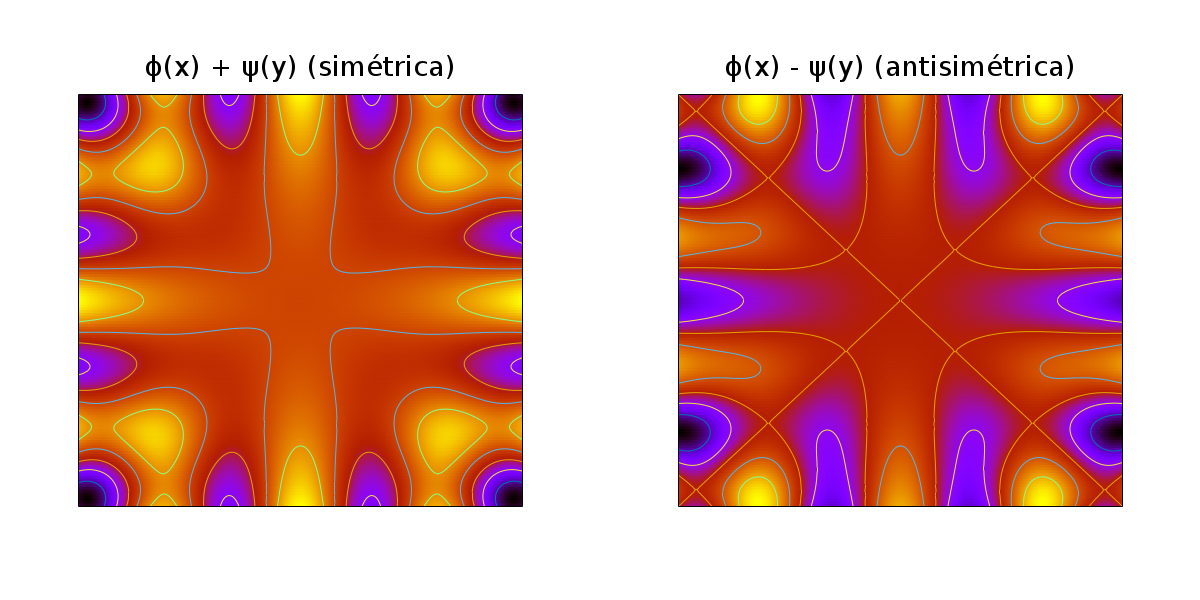
\includegraphics[width=\textwidth]{figures/simetry.png}
  \caption{Aspecto de una función de ondas simétrica y de una función de
    ondas antisimétrica}
  \label{fig:simetry}
  \forceversofloat
\end{figure}

Al ser el hamiltoniano simétrico\footnote{Al ser las partículas
  idénticas, las permutaciones de índices no deben tener un efecto
  real en las mediciones.} una función de ondas conserva su
simetría, como puede verse analizando la ecuación de Schrödinger ($i
\hbar \pdv{t} \psi =  \Ham \psi$).

\section{Partículas no elementales}
A veces es complicado definir
``partícula'', al no existir certeza absoluta sobre la ausencia de
estructura interna. Puede evitarse ese problema suponiendo al objeto
una partícula elemental y utilizando como espín el momento angular
total respecto al centro de masas, $J^*$; el hidrógeno, por ejemplo,
se comporta como una partícula elemental de espín
$s=J^*=\nicefrac{1}{2}\otimes\nicefrac{1}{2}\otimes l$. Al ser $l$
entero, el espín queda entero y se comporta como un bosón. De esta
forma, obtenemos los mismos resultados al permutar dos átomos de hidrógeno 
consideremos o no la estructura interna:
\begin{align}
  \psi &=
  \psi(\underset{p}{1},\underset{e^-}{2},\underset{p}{3},\underset{e^-}{4})
  \ \stackrel{1 \leftrightarrow 3}{\rightarrow} \ -\psi(3,2,1,4)  \
  \stackrel{2 \leftrightarrow 4}{\rightarrow} +\psi(3,4,1,2) \\
  \psi &=
  \psi(\underset{\text{H}_1}{1},\underset{\text{H}_2}{2})
  \ \stackrel{1 \leftrightarrow 2}{\rightarrow} \ +\psi(2,1)
\end{align}

%Redactar como una persona
Como ejemplos en la naturaleza tenemos el deuterio, el \textsuperscript{3}He
(ambos fermiones) y el \textsuperscript{4}He (un
bosón).\jokemargin{El \textsuperscript{3}He ha sido declarado recurso estratégico,
  de forma que EEUU ya lo ha acaparado. El Ministerio de Energía lo
  tiene todo y solo lo suelta bajo juramento y... bueno, ya sabéis
  cómo funciona el imperio\index{imperio}, para qué os voy a aburrir. Lo hizo Roma,
  lo hicimos nosotros, lo hizo Inglaterra y ahora lo hace EEUU.}
\section{Determinante de Slater}\index{Slater, determinante}
Sea un hamiltoniano $ \Ham (1,2,3) = h(1) +
h(2) + h(3)$. Sean $E_u,E_v,E_w$ los autovalores de $ \Ham $
con autoestados correspondientes $u,v,w$. Hay $3!$ autoestados
$u(i)v(j)w(k)$; si las partículas son bosones no hay más que sumarlos,
si son fermiones podemos utilizar el determinante de Slater para
obtener rápidamente la función de ondas antisimétrica:
\begin{equation}
  \Psi_\text{ant.} \propto
  \begin{vmatrix}
    u(1) & u(2) & u(3) \\
    v(1) & v(2) & v(3) \\
    w(1) & w(2) & w(3) 
  \end{vmatrix} = u(1)v(2)w(3) - \cdots
\end{equation}
Notar que hay que determinar la norma de la función resultante, que no
es más que $\sqrt{3!}$ al escogerse\footnote{No siempre tiene por qué ser así} autoestados
ortogonales. Si bien el
método es generalizable sin más que utilizar un determinante mayor a
sistemas de $N$ partículas, solo es válido cuando el hamiltoniano es
separable (las partículas son independientes):
\begin{equation}
  \Psi_\text{ant.} = \frac{1}{\sqrt{N!}}
  \begin{vmatrix}
    \varphi_1(1) & \cdots & \varphi_1(N) \\
    \vdots & \ddots & \vdots \\
    \varphi_N(1) & \cdots & \varphi_N(N) \\
  \end{vmatrix} 
\end{equation}
De aquí se deduce el \emph{principio de exclusión de Pauli}. Si dos
columnas son iguales (dos partículas están en el mismo estado) el
determinante se anula y la probabilidad de que el sistema esté en ese
estado cuántico es nula.
\section{Degeneración de intercambio}
Consideremos dos partículas idénticas no independientes, con
hamiltoniano $ \Ham (1,2) =  \Ham (2,1) \neq h(1) + h(2) $
simétrico. Obtenemos la siguiente ecuación de autovalores:
\begin{equation}
     \Ham (1,2) \varphi(1,2) = E \varphi(1,2)
\end{equation}
Puedo permutar los índices sin cambiar la energía:
\begin{equation}
     \Ham (2,1) \varphi(2,1) = E \varphi(2,1)
\end{equation}
Pero como el hamiltoniano es simétrico,
\begin{equation}
     \Ham (1,2) \varphi(2,1) = E \varphi(2,1)
\end{equation}
vemos que $ \Ham $ tiene por tanto dos autoestados con la misma
energía, $\varphi(1,2)$ y $\varphi(2,1)$. A esta degeneración se le denota
\emph{degeneración de intercambio} para diferenciarla de otras
degeneraciones como la que aparece de manera natural en un oscilador
armónico 2D.

%%% Local Variables:
%%% mode: latex
%%% TeX-master: "../resumen"
%%% End:

\chapter{El átomo de helio}
Es un ejemplo de problema de tres cuerpos, no resoluble
analíticamente. En CGS\footnote{Sistema basado en el gramo, el segundo
y el centímetro. La ley de Coulomb es simplemente $1\cdot\frac{qq'}{r^2}$,
donde la distancia está en centímetros y la carga en \emph{estatculombios}.} el hamiltoniano se escribe como
\begin{equation}
   \Ham  = \frac{-\hbar^2}{2m} \nabla_1^2 - \frac{\hbar^2}{2m}
  \nabla_2^2 - \frac{Ze^2}{r_1} - \frac{Ze^2}{r_2} + \frac{e^2}{r_{12}}
  \label{eq:heliumh}
\end{equation}
donde $Z=2$ en el helio. Para el Li\textsuperscript{+} vale $Z=4$,
para el Be\textsuperscript{++} cinco, etc. Estamos suponiendo que la
masa del núcleo es mucho más grande que la masa del electrón.

Es un hamiltoniano de partículas idénticas, ya que permutar los
índices no lo varían. No obstante, hay un término de interacción que
no es eliminable por ser del mismo orden de magnitud\footnote{
Si comparamos los niveles experimentales del helio con el
    modelo suponiendo nulo el término de interacción
    electrón-electrón, vemos que la aproximación es mala:
    \begin{center}
      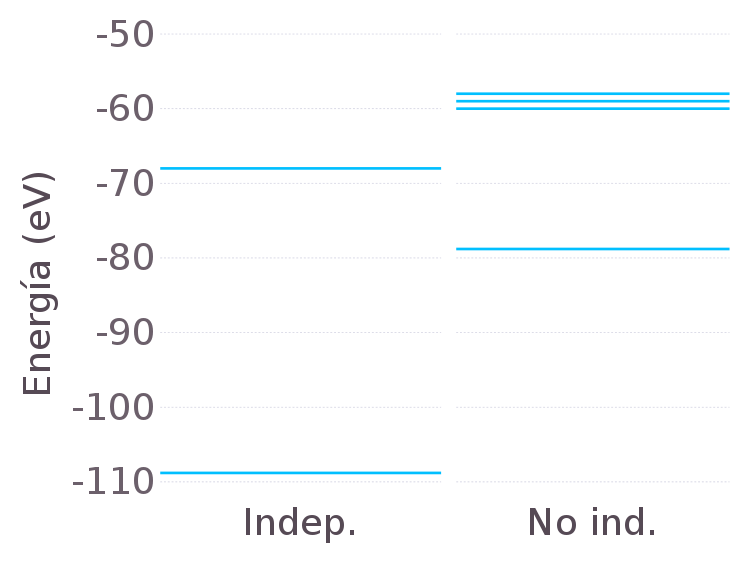
\includegraphics[width=0.4\textwidth]{figures/helium_noint.png}
    \end{center}
Los niveles en el caso de partículas independientes vienen dados
por \[E_{nn'} = -136 \left( \frac{Z^2}{n^2} + \frac{Z^2}{n'^2}
  \right) \text{ eV}\]
}. No obstante, podemos tratarlo como una perturbación para obtener
resultados analíticos.

La función de ondas resultante de esta aproximación ha de ser antisimétrica,
\begin{equation}
  \psi \propto \varphi_{n\ell m\mu}(1)\varphi_{n'l'm'\mu'}(2) - \varphi_{n\ell m\mu}(2)\varphi_{n'l'm'\mu'}(1)
\end{equation}
donde los números entre paréntesis indican en qué coordenadas evaluar las
funciones de ondas. Por ejemplo, $R(1)$ es notación para $R(r_1)$ y
$Y_{-1}^{1}(3)$ significa $Y_{-1}^1 (\Omega_3)$.

El factor de normalización de la función de ondas es simplemente
$\frac{1}{\sqrt{2}}$, ya que las $\varphi_i$ son ortogonales con las
$\varphi_{i'}$. En el caso en que los números cuánticos son iguales la
función de ondas ya no tiene esa norma (al no ser las $\varphi$
ortogonales, sino iguales), pero dichas funciones de onda están
prohibidas por el postulado de simetrización\footnote{En el caso de
  partículas no interactuantes, se puede recurrir al principio de
  exclusión de Pauli.}; el determinante de
Slater correspondiente tendría dos columnas iguales y sería nulo,
dando como resultado una función de ondas de norma nula.

\section{Nivel fundamental}
La función de ondas de este nivel, en la aproximación de electrones no
interactuantes, es
\begin{equation}
  \psi = \frac{1}{\sqrt{2}} [\varphi_{100\oh}(1) \varphi_{100\moh}(2)
  - \varphi_{100\oh}(2) \varphi_{100\moh}(1)]
\end{equation}
No hay degeneración. Podemos escribir $\psi$ como
\begin{equation}
  \begin{split}
    \psi &= \frac{\varphi_{100}(1)\varphi_{100}(2)}{\sqrt{2}}
    ( \ket{+}_1\ket{-}_2 - \ket{-}_1\ket{+}_2 ) \\
    &= \varphi_{100}(1)\varphi_{100}(2) \chi_0^0(1,2)
  \end{split}
\end{equation}
donde se ha utilizado una tabla de Clebsch-Gordan para escribir $
\frac{1}{\sqrt{2}}( \ket{+}_1\ket{-}_2 - \ket{-}_1\ket{+}_2 ) =
\chi_0^0(1,2)$. Vemos que hay simetría en la parte espacial y
antisimetría en la parte de los espines, de forma que la función de
ondas total es antisimétrica.

\subsection{Aproximación perturbativa}
Supongamos que el término $\frac{e^2}{r_{12}}$ es una perturbación.
Calculamos la corrección en primer orden a la energía del nivel
fundamental, el cual no es un nivel degenerado:
\begin{equation}
  \begin{split}
    \Delta E^{(1)} &=
    \ev{\frac{e^2}{r_{12}}}{\varphi_{100}(1)\varphi_{100}(2)\chi_0^0(1,2)} =
    \\
    &=
    \ev{\frac{e^2}{r_{12}}}{\varphi_{100}(1)\varphi_{100}(2)}\cancelto{1}{\ip{\chi_0^0(1,2)}}
    =\\ &=\cdots
  \end{split}
\end{equation}

Es muy incómodo trabajar con $r_{12}$ porque es un vector que no parte
del origen. Utilizando resultados de la electroestática clásica
escribimos:
\begin{equation}
  \frac{1}{r_{12}} = \sum_{\ell=0}^\infty \frac{r_<^\ell}{r_>^{\ell+1}} \text{P}_\ell(\cos\alpha)
\end{equation}
donde $r_<$ y $r_>$ son respectivamente el menor y el mayor de $r_1,r_2$
y $\text{P}_\ell$ es el polinomio de Legendre de orden $\ell$, que puede
escribirse en función de los armónicos esféricos como
\begin{equation}
  \text{P}_\ell (\cos \alpha) = \frac{4\pi}{2\ell+1} \sum_{m=-\ell}^l
  Y_\ell^{m*}(\Omega_1) Y_\ell^{m}(\Omega_2)
\end{equation}

A pesar de
haber eliminado $r_{12}$ de la integral tenemos que resolver una suma
infinita. Escribimos la parte espacial de la función de ondas como
\begin{equation}
  \varphi_{100}(\boldrm{r}_1) \varphi_{100}(\boldrm{r}_2) = \frac{Z^3}{\pi
    a_0^3} e^{\frac{-Z}{a_0}(r_1+r_2)}
\end{equation}
La integral, con todas las sustituciones, queda como
\begin{equation}
  \begin{split}
    \cdots &= \left( \frac{Z^3}{\pi a_0^3} \right)^2 e^{2}
    \iint_0^\infty r_1^2\dd{r_1}r_2^2\dd{r_2} \sum_{\ell=0}^\infty
    \frac{r_<^\ell}{r_>^{\ell+1}} e^{-2Z(r_1+r_2)/a_0} \cdot \\ &\cdot\sum_{m=-\ell}^\ell
    \frac{4\pi}{2\ell+1}\int_{4\pi} Y_\ell^{m*}(\Omega_1) \dd{\Omega_1}
    \int_{4\pi} Y_\ell^{m}(\Omega_2) \dd{\Omega_2} = \cdots
  \end{split}
\end{equation}
La integral contiene a dos armónicos esféricos ortogonales, así que
solo será no nula si $\ell=m=0$:
\begin{equation}
  \int_{4\pi}Y_\ell^{m*}(\Omega_1) \dd{\Omega_1} = \int_{4\pi}
  Y_\ell^m(\Omega_2) \dd{\Omega_2} = \sqrt{4\pi} \delta_{\ell0} \delta_{m0}
\end{equation}

Con ello, obtenemos:
\begin{equation}
  \cdots = \left( \frac{Z^3}{\pi a_0} \right)^2 e^{2} 16 \pi^2
  \iint_0^\infty r_1^2 \dd{r_1} r_2^2 \dd{r_2} \frac{1}{r_>}
  e^{-2Z(r_1+r_2)/a_0} = \cdots
\end{equation}
El siguiente paso es sustituir $r_>$ por la $r$ correspondiente en
cada región de integración. En $\int_0^\infty \dd{r_1} \int_0^{r_1} \dd{r_2}$ el mayor $r$
es $r_2$, y en $\int_0^\infty \dd{r_1} \int_{r_1}^\infty \dd{r_2}$ el
mayor pasa a ser $r_1$; conocido esto obtenemos:
\begin{equation}
  \begin{split}
    \cdots &= \left( \frac{Z^3}{\pi a_0} \right)^2 e^{2} 16
    \pi^2\int_0^\infty r_1^2 \dd{r_1} \Big[ \int_0^{r_1} \dd{r_2}
      \frac{1}{r_1} r_2^2 e^{-2Z(r_1+r_2)a_0} + \\ &+ \int_{r_1}^\infty
      \dd{r_2} \frac{1}{r_2} r_2^2 e^{-2Z(r_1+r_2)a_0} \Big] 
  \end{split}
\end{equation}

resolviendo las integrales resultantes, finalmente obtenemos
\begin{equation}
  \Delta E^{(1)} = \frac{5}{128} \frac{a_0^5}{Z^5}
  \stackrel{\text{He}}{=} \SI{34}{\eV}
\end{equation}
Vemos que la corrección es grande. El valor corregido (\SI{-74.8}{\eV})
es similar\jokenote{Que sean más o menos iguales depende de la
  escala, pero da igual porque la energía no es trabajo, que es lo que
es dinero. Y la pela es la pela, incluso en Panamá.} al experimental (\SI{-79}{\eV}).

\subsection{Aproximación variacional}

Ahora que conocemos la energía, podemos estimar la función de ondas
del nivel fundamental con el método variacional. Utilizamos una
función de prueba con un parámetro $\alpha$:
\begin{equation}
  \psi = \underbrace{\frac{\alpha^3}{\pi a_0^3} e^{-\alpha(r_1+r_2)/a_0}}_{\text{simmetric}} \underbrace{\chi_0^0(1,2)}_{\text{ant.}}
\end{equation}
$\alpha$ hace las veces de $Z$; de esta forma suponemos que bajo la
interacción los electrones se comportan como si fueran independientes
pero en un potencial central distinto a $Z=2$. Separamos $\psi$ en la
parte espacial y la de espín:
\begin{equation}
  \varphi =
  \varphi_{100}(\boldrm{r}_1,\alpha)\varphi_{100}(\boldrm{r}_2,\alpha) \chi_0^0
\end{equation}
Las $\varphi$ están en un potencial de Coulomb con $Z=\alpha$. Su forma
funcional es
\begin{equation}
  \varphi_{100}(\boldrm{r},\alpha) = \left( \frac{\alpha^3}{\pi a_0^3}
  \right)^{\oh} e^{-\alpha r /a_0}
\end{equation}
Las $\varphi$ son autoestados de $\frac{-\hbar^2}{m}\nabla^2 -\alpha
\frac{e^2}{r}$ con autovalor $\frac{-1}{2}\frac{e^2}{a_0}\alpha^2$.
Calculamos $\ev{ \Ham }{\psi}$ para tratar de minimizarlo, de esa
forma hallaremos la $\psi$ más parecida a $\psi_0$. Analizemos por
separado cada integral del hamiltoniano del helio \eqref{eq:heliumh}:
\begin{itemize}
\item Comenzamos por el término cinético:
  \begin{equation}
    \begin{split}
      \ev{\frac{-\hbar^2}{2m}\nabla_1^2}{\psi} &=
      \ev{\frac{-\hbar^2}{2m}\nabla_1^2}{\varphi_{100}(\boldrm{r}_1,\alpha)}
      \cdot \\ &\cdot \underbrace{\ip{\varphi_{100}(\boldrm{r_2},\alpha)}}_{=1}
      \underbrace{\ip{\chi_0^0}}_{=1}
    \end{split}
  \end{equation}
  Utilizando el teorema del virial obtenemos $\langle T \rangle = -E =
  \frac{+1}{2} \frac{e^2}{a_0} \alpha^2$. Con el término cinetico de
  la otra partícula ocurre lo mismo.
\item El término de potencial central resulta:
  \begin{equation}
    \begin{split}
      \ev{\frac{Ze^2}{r}}{\psi} &=
      \ev{\frac{-Ze^2}{r_1}}{\varphi_{100}(\boldrm{r}_1,\alpha)} \cdot \\
      &\cdot \underbrace{\ip{\varphi_{100}(\boldrm{r_2},\alpha)}}_{=1}
      \underbrace{\ip{\chi_0^0}}_{=1} = \\
      &= \frac{Z}{\alpha} \langle V \rangle
      \stackrel{\text{virial}}{=} \frac{Z}{\alpha} \underbrace{2 \left( \frac{-1}{2}\frac{e^2\alpha}{a_0} \right)}_{2E_0}
    \end{split}
  \end{equation}
\item Por último, calculamos\footnote{Se deja como ejercicio para el
    estudiante.} el término de interacción.
\begin{equation}
  \ev{\frac{e^2}{r_{12}}}{\psi} = \cdots = \frac{5}{8} \frac{\alpha e^2}{a_0}
\end{equation}
\end{itemize}

Si juntamos los resultados, obtenemos
\begin{equation}
  \ev{ \Ham }{f(\alpha)} = \frac{e^2}{a_0} \left(\alpha^2 -2Z\alpha +
    \frac{5}{8}\alpha \right)
\end{equation}
Vemos que el mínimo está en $\alpha = Z - \nicefrac{5}{16}$, con valor
$\SI{-77.5}{\eV} \geq E_0$ ($Z=2$). El valor experimental es
\SI{-78.8}{\eV}, y el perturbativo era \SI{-74.8}{\eV}. Como
$\eval{E_\text{var.}}_\text{min} \simeq E_\text{exp.}$ es plausible\jokenote{Tan plausible como que no tenemos otra.} que
$\psi(\alpha_\text{min}) \simeq \psi_0$. Por tanto, tenemos una
indicación de que es conveniente utilizar $Z=2-\nicefrac{5}{16}$ en
lugar de $Z=2$.

Con funciones de ondas más complicadas y más parámetros se pueden
sacar energías más cercanas a $E_0$ (y por tanto ajustar mejor
$\psi_0$). Hylleraas\historynote{Egil Andersen Hylleraas (1898-1965) fue un distinguido físico teórico
noruego conocido por su método simple pero elegante para predecir el
estado energético fundamental de átomos de dos electrones, así como
funciones de onda de prueba de átomos multielectrónicos. Hylleraas era
el nombre de la granja en que nació.} realizó un análisis especialmente
minucioso, obteniendo una diferencia con $E_0$ en la sexta cifra significativa.

\section{Niveles excitados}
Definimos un potencial central virtual $V(r)$ que nos permite escribir
el hamiltoniano del sistema como
\begin{equation}
  \begin{split}
     \Ham  = -\frac{\hbar^2}{2m}\nabla_1^2 -
      \frac{\hbar^2}{2m}\nabla_2^2 &+ V(r_1) + V(r_2)
    - \\
    &- V(r_1) - V(r_2) - \frac{\alpha e^2}{r_1} - \frac{\alpha
      e^2}{r_2} + \frac{e^{2}}{r_{12}} 
  \end{split}
\end{equation}

De esta manera tenemos el hamiltoniano expresado como un hamiltoniando
de partículas idénticas e independientes: 
\begin{align}
 \Ham _0 &= \frac{-\hbar^2}{2m}\nabla_1^2 - \frac{\hbar^2}{2m} \nabla_2^2 + V(r_1)
+ V(r_2) = h_1+h_2 \\
                W &=  - V(r_1) - V(r_2) - \frac{\alpha e^2}{r_1} - \frac{\alpha
      e^2}{r_2} + \frac{e^{2}}{r_{12}} \ll  \Ham _0
\end{align}
Cada partícula independiente cumple con $ \Ham _0$ la siguiente
ecuación de autovalores:
\begin{equation}
  \left[ \frac{-\hbar^2}{2m} + V(r) \right] \varphi_{n\ell m\mu}(\boldrm{r})
  = E_{nl} \varphi_{n\ell m\mu}(\boldrm{r})
\end{equation}
donde $\varphi_{n\ell m\mu}(\boldrm{r}) = R_{nl}(r) Y_l^m(\Omega)\ket{\oh\
  \mu}$, y el CSCO es $ \Ham ,L^2,L_z,S_z$.

Resolvemos la parte radial expresando $ \Ham _0$ en coordenadas
radiales en la ecuación de Schrödinger:
\begin{equation}
  \left[ \frac{-\hbar^2}{2m} \dv[2]{r} + V(r) + \frac{\ell (\ell+1)
      \hbar^2}{2mr^2}\right] = \chi_{n\ell}(\boldrm{r}) = E_{n\ell} \chi_{n\ell}(r)
\end{equation}
donde $\chi_{nl} = r R_{nl}$. El valor de $\ell$ cambia el tipo de
ondas que obtenemos como autoestados. Con $\ell =0$ obtenemos ondas de
tipo \emph{s} y energías $E_{1s},E_{2s},\ldots$, con $\ell = 1$ las
ondas son \emph{p} y las energías $E_{2p},E_{3p},\ldots$ etc. Se ha utilizado
el convenio de física atómica, donde se expresa la mínima $n$ como
$\ell +1$.

Los autovalores de $ \Ham _0$ serán $E_{nl}+E_{n'l'}$, al ser
partículas independientes. En notación de números de ocupación, los
autovalores son $(n\ell)^1(n'\ell')^1$. Los autoestados serían, en
principio,
$\varphi_{n\ell m\mu}(\boldrm{r}_1)\varphi_{n'\ell'm'\mu'}(\boldrm{r}_2)$, pero
necesitamos antisimetrizar la función de ondas por ser los electrones
fermiones:
\begin{equation}
  \Psi \propto  
\varphi_{n\ell m\mu}(\boldrm{r}_1)\varphi_{n'\ell'm'\mu'}(\boldrm{r}_2) - \varphi_{n\ell m\mu}(\boldrm{r}_2)\varphi_{n'\ell'm'\mu'}(\boldrm{r}_1)
\end{equation}


\subsection{Degeneración de los niveles}
\label{subsection:deglevel}

La degeneración de la energía para $E_{n\ell}\neq E_{n'\ell'}$ es distinta
que para el caso $E_{n\ell} = E_{n'\ell'}$:
\begin{itemize}
\item Si las energías son distintas,
 la degeneración corresponde al
  número de determinantes de Slater que podemos construir. Para
  construir un determinante de Slater necesitamos que los números
  cuánticos no sean exactamente iguales; dado un $\ell$ tenemos $2\ell +1$
  números distintos para la $m$ y $2s+1$ números para la $\mu$.
  Como el espín vale $\oh$ tenemos que $\mu = \pm \oh$, y tenemos que
  la degeneración es
  \begin{equation}
    g = \underbrace{(2\ell +1)}_{g_\ell} \cdot \underbrace{2}_{g_\mu} \cdot
    \underbrace{(2\ell' +1)}_{g_\ell'} \cdot \underbrace{2}_{g_\mu'}
  \end{equation}
\item Si las energías son iguales, los números cuánticos $\ell,\ell'$
  son idénticos y solo podemos variar $m,\mu$. Para $\ell=1$, por
  ejemplo, disponemos de seis\footnote{Concretamente,
    $m\in -\ell,\cdots,\ell$ y $\mu = \pm \oh$:
  \begin{center}
    \begin{tabular}{c|c}
     $\mu$ & $m$ \\ \hline
      $+\oh$ & $+1$ \\ 
      $+\oh$ & $\ \ 0$ \\ 
      $+\oh$ & $-1$ \\ 
      $-\oh$ & $+1$ \\ 
      $-\oh$ & $\ \ 0$  \\ 
      $-\oh$ & $-1$ \\ 
    \end{tabular}
  \end{center}
}
parejas de valores:
Tenemos que escoger grupos de dos parejas distintos para los estados.
Por ejemplo, $\ket{m\mu}=\ket{+1\ +\oh}$ y $\ket{m'\mu'}=\ket{0\ -\oh}$.
Hay seis parejas $(m,\mu)$ distintas, así que podemos escoger
$g=\binom{6}{2}$ estados distintos. Para $\ell$ genérica, la
degeneración será
\begin{equation}
  g = \binom{(2\ell + 1)\cdot 2}{2}
\end{equation}
\end{itemize}

Vemos que la degeneración puede crecer mucho, por lo que es importante
escoger buenas bases. 

\paragraph{Ejemplos}
\begin{itemize}
\item $E_{1s}+E_{2s} \ \rightarrow \ (1s)^1(2s)^1$. Las energías son
  distintas, así que hay $2\cdot(2\ell+1)\cdot 2 \cdot (2\ell'+1)$
  estados distintos. Como los orbitales \emph{s} se caracterizan por
  tener un número cuántico $\ell$ nulo, nos queda $2\cdot(0+1)\cdot 2
  \cdot (0+1)$ y obtenemos $g=4$.
\item $E_{1s}+E_{2p} \ \rightarrow \ (1s)^1(2p)^1$. En este caso
  aparece un orbital \emph{p}, con $\ell = 1$. Obtenemos $2\cdot(0+1)\cdot 2
  \cdot (2\cdot 1+1)$, y por tanto $g = 12$.
\item $2E_{1s} \ \rightarrow \ (1s)^2$. Las energías son iguales, así
  que la degeneración vendrá dada por $\binom{(2\ell +1)\cdot 2}{2}$.
  Como $\ell =0$, tenemos $g=\binom{2}{2}=1$.
\item $2E_{1p} \ \rightarrow \ (1p)^2$. En este caso $\ell =1$ y obtenemos 
  $g=\binom{2(2\cdot1 +1)}{2}=\binom{6}{2}=15$.
\end{itemize}

\subsection{Diagonalización de $W$}
Recordamos que
\begin{equation}
  W = -V(r_1) - V(r_2) - \frac{Ze^2}{r_1} - \frac{Ze^2}{r_2} + \frac{e^2}{r_{12}}
\end{equation}
No conmuta con rotaciones de una sola partícula\footnote{Es obvio, ya
  que si rotamos solo una partícula puede cambiar la distancia
  $r_{12}$ entre ambas.}, $\boldrm{L}_i$,
pero sí con rotaciones del sistema, $\boldrm{L} =
\boldrm{L}_1+\boldrm{L}_2$. $W$ no depende de los espines, así que
conmuta con todos sus operadores. En resumen, 
\begin{equation}
  [W,\boldrm{L}]=[W,\boldrm{S}]=[W,L_z]=[W,L^2] = 0
\end{equation}
Es posible que $L^2,L_z,S^2,S_z$ sean un CSCO para las
funciones antisimétricas del subespacio de degeneración
$E_{n\ell}+E_{n'\ell'}$, pero existe ambiguedad en la función. 
Sean dos parejas fijas de
números cuánticos $(n\ell)$ y $(n'\ell')$, los coeficientes de
Clebsch-Gordan nos dan dos funciones globales para el sistema,
$F_{\ell\ell'}\ket{M_L\ L}(\boldrm{r}_1,\boldrm{r}_2)$ y la
permutación $F_{\ell\ell'}\ket{M_L\ L}(\boldrm{r}_2,\boldrm{r}_1)$,
que pueden ser simétricas ($L$ par) o antisimétricas ($L$ impar).
Además, como parte de espín, podemos escoger\footnote{No hay más combinaciones, ya
  que con espín $\oh$ podemos obtener únicamente las combinaciones
  dadas por $\frac{1}{2} \otimes \frac{1}{2} = 0,1$. La demostración
  de que $S=0$ es antisimétrica y $S=1$ simétrica es inmediata
  escribiéndolos como combinación lineal en la base de
  $\ket{\pm}_1,\ket{\pm}_2$ con las tablas de Clebsch-Gordan y viendo
  que pasa al permutar los índices.} tanto  $\chi_0^0(1,2)$ (antisimétrica) y
$\chi_1^{M_S}(1,2)$ (simétrica). Esto nos da una degeneración doble
por la elección del espín,
pero es solventable con el postulado de simetrización. Escribimos
ambas posibles funciones del sistema como
\begin{equation}
  \Psi =
  \begin{cases}
&F_{\ell\ell'} {M_L \atop L}(\boldrm{r}_1,\boldrm{r}_2) \chi_0^0(1,2)\ 
\pm  \
F_{\ell\ell'}{M_L\atop L}(\boldrm{r}_2,\boldrm{r}_1) \chi_0^0(1,2) \\
&F_{\ell\ell'} {M_L \atop L}(\boldrm{r}_1,\boldrm{r}_2) \chi_1^{M_S}(1,2)\ 
\pm  \
F_{\ell\ell'}{M_L\atop L}(\boldrm{r}_2,\boldrm{r}_1) \chi_1^{M_S}(1,2) 
  \end{cases}
  \label{eq:psicases}
\end{equation}

donde el $\pm$ depende de si la función $F$ era simétrica o
antisimétrica\footnote{Si son simétricas basta con sumarlas, si son
  antisimétricas hemos de restar su permutación.}.
Vemos que hay dos elecciones posibles debido a $\chi$, pero que $\Psi$ tenga que ser
antisimétrica lo soluciona.
\begin{itemize}
\item Si $L$ es par, la función $F_{\ell\ell'}{M_L \atop L}$ ha de tener parte de espín antisimétrica,
  $\chi_0^0(1,2)$. De esta forma, obtenemos $\text{sim}\otimes
  \text{antisim} = \text{antisim}$.
\item Si por el contrario $L$ es impar, la función ha de tener parte
  de espín par, $\chi_1^{M_S}(1,2)$. Así se obtiene $\text{antisim}\otimes
  \text{sim} = \text{antisim}$.
\end{itemize}

De esta forma podemos escoger uno de los dos casos de la
ecuación \eqref{eq:psicases}, y vemos que el CSCO es realmente
completo. Notar que todo este tratamiento es válido únicamente para
sistemas de
dos partículas. Obtenemos una representación matricial completamente
diagonal para $W$:
\begin{equation}
  \ev{W}{\Psi} \sim
  \delta_{\ell\ell'}\delta_{M_L M_L'}\delta_{S^2 S'^2}\delta_{M_S M_S'}
\end{equation}
donde $\ket{\Psi}  = \ket{(n\ell)(n'\ell')L\ M_L\ S\ M_S}$.

En principio se tendría que calcular todos los valores de la diagonal,
pero como se vio en los ejercicios\footnote{Estructura fina del hidrógeno,
  sección de la página \pageref{paragraph:l0vm}, ecuación \ref{eq:exercises_recurrence}}
el hecho de que $[V,\boldrm{J}]=\boldrm{0}$ implica que $\ev{V}{\alpha j m}
= \ev{V}{\alpha j m\pm 1}$. En principio no esperamos que aparezca el
espín, pero lo tenemos en cuenta. 

\subsection{Términos espectroscópicos}
Tenemos energías del estilo $E = E_{n\ell}+E_{n'\ell'}+\Delta(n\ell n'\ell' L S)$. Si
solo indicamos la configuración, $(nl)(n'\ell')$, solo damos
información sobre $\Ham$ (en $n$) y $L^2$ (en $\ell$). El CSCO requiere
de más observables para ser completo, así que introducimos los
llamados \emph{términos espectroscópicos} para dar información sobre
los observables $L_z,S^2$ y completar el CSCO\footnote{Aún falta
  información sobre $S_z$, por lo que las configuraciones con término
  espectroscópico pueden seguir estando degeneradas.}.

Como ejemplo práctico, veamos la configuración $(1s)(2s)$. Tenemos un
valor único para $L$ en $0\otimes0 = \{0_S\}$ y dos para el observable espín
total, $S\in \oh \otimes \oh = \{0_S,1_A\}$, donde el subíndice indica si la
función es simétrica o no. Tenemos por tanto dos parejas, $\ket{L:0\
  S:0}$ y $\ket{L:0 \ S:1}$, para indicarlas introducimos un término
 extra ${}^{2S+1}L$, que nos da información del
momento angular orbital (en este caso sólo puede ser nulo) y el espín
total (uno o cero). Se utiliza la notación $S=0,P=1,D=2,F=3,\ldots$
para indicar $L$. Así pues, identificamos $\ket{L:0\ S:0}$ con un
estado \emph{singlete} ${}^{1}\!S$ y $\ket{L:0\ S:1}$ con ${}^3\!S$ 
(\emph{triplete}). La degeneración de cada subestado es simplemente
$2S+1$, como puede verse en el diagrama de niveles de la figura \ref{fig:uncoupling}.


\begin{marginfigure}
  \begin{tikzpicture}[xscale=1.5,yscale=1]
    \draw[blue, ultra thick] (0,1) -- (1.5,1);
    \draw[blue, thin, dashed] (1.5,1) -- (2,2);
    \draw[blue, thick] (2.05,2) -- (3,2);
    \draw[blue, thin, dashed] (1.5,1) -- (2,0);
    \draw[blue, thick] (2.3,0) -- (3,0);
    \draw[blue, thick] (2.3,0.5) -- (3,0.5);
    \draw[blue, thick] (2.3,-0.5) -- (3,-0.5);
    \draw[blue, thin, dashed] (2.05,0) -- (2.3,0);
    \draw[blue, thin, dashed] (2.05,0) -- (2.3,0.5);
    \draw[blue, thin, dashed] (2.05,-0) -- (2.3,-0.5);
    \draw node [above] at (0.5,1) {$E_{n\ell}+E_{n'\ell'}$};
    \draw node [right] at (3,2) {${}^1\!S$};
    \draw node [right] at (3,0) {${}^3\!S$};
  \end{tikzpicture}
  \caption{Degeneración de los niveles del helio}
  \label{fig:uncoupling}
\end{marginfigure}

Notar que obtenemos la misma degeneración ($1+3$) que si aplicamos las
fórmulas de \ref{subsection:deglevel}

\paragraph{Términos espectroscópicos}
Cada nivel $E_{n\ell}+E_{n'\ell'}$ tendrá como degeneración el número de
parejas $L,S$. Por ejemplo, para el nivel $(1s)(2s)$ tenemos
que $L\in\{0\otimes0\}=\{0_S\}$ y
$S\in\{\oh\otimes\oh\}=\{0_A,1_S\}$. El estado electrónico no queda
completamente determinado con la notación $(1s)(2s)$, lo que nos hace
incluir un término extra ${}^{2S+1}L$, que nos da información\footnote{El CSCO completo requiere de
  $L^2,L_z,S^2,S_z$,y el término espectroscópico añade información
  sobre $S_z$. Por ejemplo, el estado $(1s)(2s)\ {}^3\!S$ está triplemente
degenerado, ya que falta por indicar $S_z$.} del
momento angular orbital (en este caso sólo puede ser nulo) y el espín
total (uno o cero). Se utiliza la notación $S=0,P=1,D=2,F=3,\ldots$
para indicar $L$. Por ejemplo, ${}^3\!S$ indica un estado
\emph{triplete}, que tiene un espín total uno y momento angular
orbital nulo.




\paragraph{Ejemplos}
\label{paragraph:examplesdegantisim}
\begin{description}
\item[(1s)(2p)] La degeneración del orbital $(1s)$ es doble (espín
  \emph{up} y \emph{down}) y la del $(2p)$ séxtuple (espín \emph{up} y
  \emph{down}, además de un factor $3$ por el momento angular
  orbital). En forma de tabla:
  \begin{center}
    \begin{tabular}{ccccc}
      deg. & $L$ & $S$ & ${}^{2S+1}\!L$ & deg. \\ \hline
      12   & $0\otimes1 = \{1\}$ & $0,1$ & ${}^{1}\!P, {}^{3}\!P$ & $3 +3\cdot 3$ \checkmark
    \end{tabular}
  \end{center}
  De forma general, la degeneración de ${}^{2S+1}\!L$ es $(2S+1)(2L+1)$.
\item[(2p)\textsuperscript{2}] Al tener ambos electrones la misma
  energía hemos de tener cuidado con que la función total sea
  antisimétrica\footnote{
    Si tenemos dos energías y dos funciones de onda espaciales distintas, como por ejemplo
    $(1s)(2p)$, la función de ondas global $\Psi(\boldrm{1},\boldrm{2})$ es
    $R_{1s}(\boldrm{1})Y_0^0(\boldrm{1})R_{2p}(\boldrm{2})Y_1^{+1}(\boldrm{2})$,
    que no es ni antisimétrica ni simétrica. Si necesitamos una
    función de ondas simétrica, podemos emplear
    $\Psi(\boldrm{1},\boldrm{2})+\Psi(\boldrm{2},\boldrm{1})$ y si la
    necesitamos antisimétrica
    $\Psi(\boldrm{1},\boldrm{2})-\Psi(\boldrm{2},\boldrm{1})$.

    En cambio, si tenemos la misma función de ondas (la misma energía), como en el caso
    $(1s)^2$, la función de ondas global es
    $R_{1s}(\boldrm{1})Y_0^0(\boldrm{1})R_{1s}(\boldrm{2})Y_0^0(\boldrm{2})$,
    que ya es simétrica. Si tratamos de antisimetrizarla, obtenemos $\Psi
    = 0$. En general, dado el orbital $(n\ell)^2$ la parte espacial de la
    función total $F_L^{M_L}$ permuta como
    \begin{center}
      \begin{tabular}{c|l}
        \text{Sim.} & $L=2\ell$ \\
        \text{Antisim.} & $L=2\ell-1$ \\
         $\cdots$      &  $\cdots$     \\
        \text{Sim.} & $L=0$ \\
      \end{tabular}
    \end{center}
}. La degeneración debería ser
  (utilizando \ref{subsection:deglevel}) $g=\binom{6}{2}=15$, y en
  efecto:
  \begin{center}
    \begin{tabular}{ccccc}
      deg. & $L$ & $S$ & ${}^{2S+1}\!L$ & deg. \\ \hline
      15   & $1\otimes1 = \{0_S,1_A,2_S\}$ & $0_A,1_S$ & ${}^{1}\!S,
                                                   {}^{1}\!D,
                                                   {}^{3}\!P$ & $1 +5+ 9$ \checkmark
    \end{tabular}
  \end{center}
  Obtenemos una matriz $15\times15$, de la que sólo tres autovalores son
  distintos. Notar que hemos dejado fuera combinaciones como $L:0_S +
  S:1_S = {}^{3}\!S$ por no ser antisimétricas.
\item[(2p)(3p)] La degeneración debería ser $36$. En efecto:
  \begin{center}
    \begin{tabular}{ccccc}
      deg. & $L$ & $S$ & ${}^{2S+1}\!L$ & deg. \\ \hline
      36   & $1\otimes1 = \{0_S,1_A,2_S\}$ & $0_A,1_S$ & ${}^{1}\!S,
                                                   {}^{1}\!D,
                                                   {}^{1}\!P$ & $1 +3+5+$ \\
       &  &  & ${}^{3}\!S,{}^{3}\!P,{}^{3}\!D$ &   $+3+9+15 $ \checkmark\\
    \end{tabular}
  \end{center}
  Vemos que el poder antisimetrizar a placer la parte espacial nos da
  muchas más posibilidades que en $(2p)(2p)=(2p)^2$. 
\end{description}



\paragraph{Integrales de intercambio}
\label{paragraph:intinterc}
Se ha visto como el término espectroscópico ${}^{2S+1}\!L$ depende del
espín. Es extraño, ya que la perturbación no depende de él. Calculemos
explícitamente la variación de energía $\Delta E$ en
\begin{equation}
  \begin{split}
    E &= E_{n\ell} + E_{n'\ell'} + \Delta(n\ell,n'\ell',L,S) = \\
    &= E_{n\ell} + E_{n'\ell'} + \\ &+ \ev{W(\boldrm{r}_1,\boldrm{r}_2)}{(n\ell)(n'\ell')LM_LSM_S}
  \end{split}
\end{equation}

Teniendo en cuenta la antisimetrización de la función (que cambia el signo
$\pm$ de la parte espacial en función de la simetría del espinor) se
obtiene:
\begin{fullwidth}
\begin{equation}
  \begin{split}
    \Delta E &=
    \ev{W(\boldrm{r}_1,\boldrm{r}_2)}{\frac{1}{\sqrt{2}}[F_L^{M_L}(\boldrm{r}_1,\boldrm{r}_2)\pm
      F_L^{M_L}(\boldrm{r}_2,\boldrm{r}_1)]\chi_S^{M_S}} = \\
    &= \ev{W(\boldrm{r}_1,\boldrm{r}_2)}{\frac{1}{\sqrt{2}}[F_L^{M_L}(\boldrm{r}_1,\boldrm{r}_2)\pm
      F_L^{M_L}(\boldrm{r}_2,\boldrm{r}_1)]}
    \underbrace{\ip{\chi_S^{M_S}}}_{=1}= \\
    &= \frac{1}{2} \ev{W}{F_L^{M_L}(\boldrm{r}_1,\boldrm{r}_2)}
    + \frac{1}{2} \ev{W}{F_L^{M_L}(\boldrm{r}_2,\boldrm{r}_1)}
    \pm \\ &\pm \left( 
    \frac{1}{2} \mel{F_L^{M_L}(\boldrm{r}_1,\boldrm{r}_2)}{W}{F_L^{M_L}(\boldrm{r}_2,\boldrm{r}_1)}
    + \frac{1}{2}
    \mel{F_L^{M_L}(\boldrm{r}_2,\boldrm{r}_1)}{W}{F_L^{M_L}(\boldrm{r}_1,\boldrm{r}_2)}  \right)
  \end{split}
\end{equation}
\end{fullwidth}

Eliminando casi toda la notación, para hacer la ecuación comprensible
para humanos:

\begin{equation}
  \begin{split}
    \Delta E &=
    \ev{W(\boldrm{1},\boldrm{2})}{\frac{1}{\sqrt{2}}[(\boldrm{1},\boldrm{2})\pm
      (\boldrm{2},\boldrm{1})]} = \\
    &= \frac{1}{2} \ev{W}{(\boldrm{1},\boldrm{2})}
    + \frac{1}{2} \ev{W}{(\boldrm{2},\boldrm{1})}
    \pm \\ &\pm
    \left( \frac{1}{2} \mel{(\boldrm{1},\boldrm{2})}{W}{(\boldrm{2},\boldrm{1})}
    + \frac{1}{2}
    \mel{(\boldrm{2},\boldrm{1})}{W}{(\boldrm{1},\boldrm{2})} \right)
  \end{split}
\end{equation}

Recordar que el signo del $\pm$ depende de la simetrización de la
función. Como las integrales son invariantes ante una transposición $1
\leftrightarrow 2$ y $W(\boldrm{1},\boldrm{2}) =
W(\boldrm{2},\boldrm{1})$, obtenemos que los cuatro sumandos son
iguales por parejas. Por tanto, $\Delta E = D \pm C$, donde $D$ es la
\emph{integral directa} y $C$ es la \emph{integral de intercambio}.

Vemos que el término de espín $\chi$ ha desaparecido, pero influye en $\Delta
E$ mediante el signo $\pm$. Si $S=0$ el signo es positivo y si $S=1$
es negativo\footnotemark; a esto se le llama \emph{correlación del intercambio con
el espín}.


En caso de ser las energías $E_{n\ell}$ y $E_{n'\ell'}$ iguales,
desaparecen los términos cruzados y $C=0$.

\section{Estructura fina}
Quedan varias interacciones en el hamiltoniano del sistema que aún no
se han tratado:
\begin{center}
  \begin{tabular}{lr}
     Término de masa& \\
     Término de Darwin& \\
    Término de
    espín-órbita&
                  $\boldrm{l}_1\boldrm{s}_1 + \boldrm{l}_2 \boldrm{s}_2$ \\
    Término de
    espín-espín&
                 $\boldrm{s}_1 \boldrm{s}_2$ \\
      Interacción del espín con
      la otra órbita  &
    $\boldrm{l}_1\boldrm{s}_2 + \boldrm{l}_2 \boldrm{s}_1$ \\
    Interacción
    órbita-órbita &
                   $\boldrm{l}_1\boldrm{l}_2$ \\
  \end{tabular}
\end{center}

Hay bastantes más que en el hidrógeno al tratarse de un sistema más
complejo. El término dominante, no obstante, es el de espín-órbita
para $Z>2$ (en el helio es dominante el de espín-espín). Además,
faltaría el término de \emph{efecto Lamb}\footnote{Acoplamiento con
  fluctuaciones del campo electromagnético del vacío} y la estructura
hiperfina (interacción con el momento magnético del núcleo).

En resumen, se tiene
\begin{equation}
  \Ham = \Ham_0 + W + W_\text{fine}
\end{equation}
donde esperamos que $W_\text{fine} \ll W$.


Sabemos que $W$ es diagonal en $\ket{n,\ell,n',\ell',L,M_L,S,M_S}$, pero
$W_\text{fine}$ no\footnote{Por ejemplo,
  $[W_\text{fine},\boldrm{L}]\neq \boldrm{0}$}; como sí que conmuta con
$\boldrm{J}$ nos planteamos utilizar la base
$\ket{n,\ell,n',\ell',L,S,J,M}$ de autoestados de $L^2,S^2,J^2,J_z$ en
$(n\ell)(n'\ell')$.\footnote{Si bien no se demuestra, $L^2,S^2,J^2,J_z$ es
  CSCO dados unos $(n\ell)(n'\ell')$ fijos, y las $\Psi$ resultantes son
  completamente antisimétricas.}

De la conmutación con $\boldrm{J}$ de $W_\text{fine}$ deducimos que
\begin{equation}
  \ev{W_\text{fine}}{(n\ell)(n'\ell')LSJM} \propto \delta_{JJ'}\delta_{MM'}
  \label{eq:conmutationef}
\end{equation}
Pero no podemos garantizar proporcionalidad con $\delta_{LL'}\delta_{SS'}$ ya
que los conmutadores no son nulos\footnote{La demostración se omite
  por ser tediosa}. La matriz no será del todo diagonal, pero sí algo;
en resumen:
\begin{align}
  W &=
  \begin{pmatrix}
    a& & & \\
     &b& & \\
     & &c& \\
     & & &\ddots \\
  \end{pmatrix} \ \ \ \text{in}\ \  \ket{(n\ell)(n'\ell')LM_LSM_S}\\
  W_\text{fine} &=
  \begin{pmatrix}
    a&\times&\times&\times \\
    \times&b&\times&\times \\
    \times&\times&c&\times \\
    \times&\times&\times&\ddots \\
  \end{pmatrix} \ \ \ \text{in}\ \  \ket{(n\ell)(n'\ell')LSJM}
\end{align}
Las $\times$ simbolizan que hay una diagonal fuerte pero algunos elementos
fuera de ella no son nulos. Es tentador sumar ambas matrices y
diagonalizar el resultado para resolver la estructura fina del helio,
pero están en distintas bases, por lo que no pueden
sumarse\jokenote{Ni Obama.}. Para poder hacerlo, veamos que $W$
es también diagonal en $\ket{(n\ell)(n'\ell')LM_LSM_S}$, de forma que estén
en la misma base. Empezamos por ver que
\begin{equation}
  [W,\boldrm{L}]=[W,\boldrm{S}]=0 \ \rightarrow \ [W,\boldrm{J}]=0
\end{equation}
Veamos cuánto valen sus elementos no nulos en la nueva base. Para
ello, utilizamos los coeficientes de Clebsch-Gordan\footnote{Recordar
  que estos coeficientes proyectan elementos de la base en
  $L^2,L_z,S^2,S_z$ a la base en $L^2,S^2,J^2,J_z$. Por ello, se
  emplea la notación $(LM_LSM_S|LSJM)$.}, efectuando el cambio


\begin{equation}
  \begin{split}
    \ket{(n\ell)(n\ell)LSJM} &\rightarrow  \underbrace{(LM_LSM_S|LSJM)}_{C_\ell}\ket{(n\ell)(n\ell)LM_LSM_S}\\
    \ket{(n\ell)(n'\ell')LSJM} &\rightarrow
    \underbrace{(LM_L'SM_S'|LSJM)}_{C_{\ell'}}\ket{(n\ell)(n\ell)LM_L'SM_S'}
  \end{split}
\end{equation}

Obtenemos que en la nueva base $\Delta E$ es
\begin{equation}
  \begin{split}
    &\mel{(n\ell)(n'\ell')LSJM}{W}{(n\ell)(n\ell)LSJM} = \\
    &= \sum_{\mathclap{M_L,M_S,M_L',M_S'}}
    C'_{\ell'}\ C_{\ell} \underbrace{\mel{(n\ell)(n'\ell')LM_L'SM_S'}{W}{(n\ell)
        (n\ell)LM_LSM_S}}_{\Delta(n\ell n'\ell'LS)\delta_{M_L,M_L'}\delta_{M_S,M_S'}}= \\
    &= \Delta E \cdot \sum_{M_L,M_S}
    \abs{\text{Clebsch-Gordan}}^2 = \Delta E \cdot 1\\
  \end{split}
\end{equation}

donde la $\Delta(n\ell n'\ell' L S)$ ha salido factor común de la suma al no
depender de los índices de esta. Vemos que los elementos de matriz de
$W$ en la nueva base son los mismos, y estamos listos para sumar ambas
matrices sin problemas.

\paragraph{Ejemplo: (1s)(2p)} La composición de $L$ resulta $L \in 0\otimes1
= \{1\}$, mientras que $S$ es $S\in \oh \otimes \oh = \{0,1\}$. La suma de
$L,S$ será\footnote{$J$ va desde $L_\text{min}=0$ hasta
  $L_\text{max}=2$ en saltos de $1$.} $J\in\{0,1,2\}$. La
degeneración de esta energía es $2\cdot 6$, así que la matriz será
$12\times12$; tendremos que calcular $144$ elementos a
priori\footnote{Sobran la mitad de los cálculos por ser la matriz hermítica}. Tenemos dos términos espectroscópicos, el ${}^{1}\!P$ y el
${}^{3}\!P$; veamos que elementos fuera de la diagonal\footnote{Por
  eso utilizamos distintos términos espectroscópicos en cada lado. Si
  no, estaríamos en la diagonal de la matriz.} no son
nulos\footnote{Para ser no nulos tenemos que tener las mismas $J,M$ a
  ambos lados (ver ecuación \eqref{eq:conmutationef}).}:
\begin{equation}
  \begin{split}
    \mel{(1s) (2p)\ {}^1\!P\ J\ M}{W_\text{fine}}{(1s) (2p)\ {}^3\!P\
      J\ M} &\neq 0\\
    \mel{
    (1s) (2p)\ {}^1\!P\ 
    \underset{1}{\overset{1}{\scriptstyle 1}} \ 
    \underset{-1}{\overset{+1}{\scriptstyle \  0}}
    }
    {
    W_\text{fine}
    }{
    (1s) (2p)\ {}^3\!P\
    \underset{1}{\overset{1}{\scriptstyle 1}} \ 
    \underset{-1}{\overset{+1}{\scriptstyle \ 0}}
    }
    &\neq 0
  \end{split}
\end{equation}
donde se ha utilizado que $J=1$ es la única $J$ que coincide en
ambos términos espectroscópicos. Vemos, por tanto, que sólo tres
elementos de fuera de la diagonal no son nulos\footnote{Más otros tres
al otro lado de la diagonal}.

Los términos de fuera de la diagonal son despreciables. Puede verse en
caso sencillo sumando a una matriz diagonal $\smqty(A&0\\ 0&B)$ una matriz
$\smqty(a&c^*\\ c &b)$ con $c\ll (a-b)^2$. 
Desarrollando en serie los
autovalores de la matriz suma vemos que las correcciones de los
elementos de la diagonal son pequeñas:
\begin{equation}
  \mqty(A& \\ & B) + \mqty(a&c^* \\ c & b) \sim \mqty(A+a & \\ & B+b)
  \label{eq:twobytwoargument}
\end{equation}

Con los valores típicos del
helio son menores de \SI{1e-7}{\eV}. A esta aproximación resultante de
suponer nulos estos elementos se le conoce
como \emph{acoplamiento LS} o de \emph{Rusell-Saunders}.

La energía a primer orden, por tanto, será
\begin{equation}
  E \simeq E_{n\ell} + E_{n'\ell'} + \Delta(n\ell n'\ell' LS) + \Delta_\text{fine}(n\ell n'\ell' LSJ)
\end{equation}
El término nuevo no depende de $M$ porque
$[W_\text{fine},\boldrm{J}]=0$. Esta energía está
degenerada $2J+1$
veces\footnote{Como $[W_\text{fine},\boldrm{J}]=0$ no depende de $M$,
  y la degeneración de $M$ es $2J+1$.}. 


Con todo lo visto, podemos razonar el desdoblamiento de un nivel como
el $(1s)(2p)$, por ejemplo (figura
\ref{fig:heliumlevelfinal}).  
Las cantidades $A,B,a,b$ de la se refieren a la ecuación
\ref{eq:twobytwoargument}.


\begin{figure}
  \begin{center}
    \begin{tikzpicture}[xscale=1.5,yscale=1]
        \draw node [above] at (0,1) {$(n\ell)(n'\ell')$};
        \draw[blue, ultra thick] (-1,1) -- (1,1);
        \draw[blue, thin, dashed] (1,1) -- (1.5,2);
        \draw[blue, thin, dashed] (1,1) -- (1.5,0);
        \draw[blue, ultra thick] (1.5,2) -- (3,2);
        \draw node [above] at (2.3,2) {${}^1\!P \text{ (singlete)}$};
        \draw[blue, ultra thick] (1.5,0) -- (3,0);
        \draw node [below] at (2.3,0) {${}^3\!P \text{ (triplete)}$};
        \draw[blue, thin, dashed] (3,2) -- (3.5,2);
        \draw[blue, thin] (3.5,2) -- (4.5,2);
        \draw node [above] at (4,2) {${}^1\!P_1$};
        \draw[blue, thin, dashed] (3,0) -- (3.5,0);
        \draw[blue, thin, dashed] (3.5,0) -- (3.8,1);
        \draw[blue, thin, dashed] (3.5,0) -- (3.8,-0.6);
        \draw[blue, thin, dashed] (3.5,0) -- (3.8,-1.2);
        %
        \draw[blue, thin] (3.8,1) --  (4.5,1)    ;
        \draw node [above] at (4,1) {${}^3\!P_0$};
        \draw[blue, thin] (3.8,-0.6) -- (4.5,-0.6)    ;
        \draw node [above] at (4,-0.6) {${}^3\!P_1$};
        \draw[blue, thin] (3.8,-1.2) -- (4.5,-1.2)    ;
        \draw node [above] at (4,-1.2) {${}^3\!P_2$};
        %
        \draw[purple,thick , <->] (2.3,2) -- (2.3,0);
        \draw node [right] at (2.3,1.2) {$\SI{0.25}{\eV}$};
        \draw node [right] at (2.3,0.8) {$A-B$};
        %
        \draw[purple,thick , <->] (4.4,1) -- (4.4,-0.6);
        \draw node [right] at (4.5,0.2) {$\SI{1.2e-4}{\eV}$};
        %
        \draw[purple,thick , <->] (4.4,-0.6) -- (4.4,-1.2);
        \draw node [right] at (4.5,-1.1) {$\ \ \ \ a'-b'$};
        \draw node [right] at (4.5,-0.8) {$\SI{1e-5}{\eV}$};
    \end{tikzpicture}
  \end{center}
  \caption{Degeneración de los niveles $(1s)(2s)$ del helio}
  \label{fig:heliumlevelfinal}
\end{figure}

\jokemargin{Y con esto y un bizcocho,
  hemos acabado el átomo de helio.}


%%% Local Variables:
%%% mode: latex
%%% TeX-master: "../resumen"
%%% End:

\chapter{Perturbaciones dependientes del tiempo}
Supongamos que el hamiltoniano tiene dependencia temporal:
\begin{equation}
  \Ham(t) = \Ham_0 + \lambda \Ham_1(t)
\end{equation}
donde $\Ham_0$ es resoluble o al menos dependiente del tiempo. La
evolución temporal de las funciones de onda vendrá dada por la
ecuación de Schrödinger, $\Ham \Psi= i \hbar \dot \Psi$.

Se considera que la perturbación empieza a influir en la
evolución del sistema en un instante $t_0$, modificando los
autoestados iniciales $\varphi_i$ para convertirlos en $\psi(t)$. La
probabilidad de medir uno de los autoestados de $\Ham(t)$ con energía
$E_f$, $\varphi_f$, será:
\begin{equation}
  P_{if}(t)=\abs{\braket{\varphi_f}{\psi(t)}}^2
\end{equation}

Expresamos dicho $\psi(t)$ en función de la base de autoestados de
$\Ham_0$,
\begin{equation}
  \psi(\boldrm{r},t) = \sum_{n} a_n(t) \exp \left( \frac{-i E_n
    }{\hbar} t \right) \varphi_n(\boldrm{r})
\label{eq:psitemp}
\end{equation}
Al coeficiente\marginnote{$a_n(t) = \braket{\varphi_n}{\psi(t=0)}$} dependiente
del tiempo, $a_n(t) e^{\frac{-iE_n}{\hbar}t}$, se le denota por comodidad $b_n(t)$ y es
equivalente a $\braket{\varphi_n}{\psi(t)}$. Si $\lambda=0$ obtenemos que $a(t) =
\text{cte.}$ y se tiene la evolución temporal habitual.

Sustituyendo \eqref{eq:psitemp} en la ecuación de Schrodinger y
simplificando se
obtiene:
\begin{equation}
  \sum_{n} i \hbar \dot{a}_n \varphi_n e^{\frac{-iE_n}{\hbar}t} = \sum_{n}  \lambda a_n \Ham_1 \varphi_n e^{\frac{-iE_n}{\hbar}t} 
\end{equation}
Resolvemos la ecuación vectorial proyectando sobre un vector
$\bra{\varphi_k}$:
\begin{equation}
  i \hbar\dot{a}_k e^{\frac{-iE_k}{\hbar}t} = \sum_{n} \lambda a_n
  e^{\frac{-iE_n}{\hbar}t} \mel{\varphi_k}{\Ham_1}{\varphi_n}
\end{equation}
donde $k\in \mathbb{Z}^+$, por lo que tenemos infinitas ecuaciones
diferenciales acopladas. Hasta aquí no se ha realizado ninguna
aproximación; efectuamos la primera, dada por
\begin{equation}
  a_k = a_k^{(0)} + \lambda a_k^{(1)} + \lambda^2 a_k^{(2)} + \ldots
\end{equation}
Sustituyendo esta aproximación y coleccionando potencias de $\lambda$
obtenemos:
\begin{equation}
  \begin{split}
    \lambda^0:\ \ & \dot{a}_k^{(0)} = 0 \\ 
    \lambda^1:\ \ & \dot{a}_k^{(1)} = \frac{1}{i \hbar} \sum_{n}
    \matrixel{\varphi_k}{\Ham_1}{ \varphi_n} a_k^{(0)} \exp \left(i\omega_{k_n} t \right) \\ 
    \lambda^2: \ \ & \cdots
  \end{split}
\end{equation}
La primera ecuación refleja el caso en que no hay perturbación,
$a^{(0)}=\text{cte.}$ Si bien es posible desarrollar la aproximación a
mayor orden que $1$, nos detendremos aquí.

Nuestras condiciones iniciales son ausencia de perturbación para $t<0$
y $\varphi_i$ conocida como estado inicial. Esto implica para las $a(t)$ que
\begin{equation}
  a_k(0)  = a_k^{(0)}(0) +\lambda a_k^{(1)}(0) + \ldots = \delta_{ki}
\end{equation}
Para $\lambda=0$ obtenemos $a_k^{(0)}(0)=a_k(0)=\delta_{ki}$.

En $a_k^{(1)}$ se obtiene, integrando desde el inicio de la
perturbación ($t=0$) hasta su final ($t=t$):
\begin{equation}
  \begin{split}
    \dot{a}_k^{(1)} &= \frac{1}{i \hbar} \matrixel{\varphi_k}{\Ham_1}{\varphi_i}
    e^{i\omega_{k_i}t}\\
    a_k^{(1)}(t) &= \frac{1}{i \hbar} \int_0^t \matrixel{\varphi_k}{\Ham_1(\tau)}{\varphi_i}
    e^{i\omega_{k_i}\tau} \dd{\tau}
  \end{split}
\end{equation}
donde $a_k^{(1)}(0)=0, \ \forall k$. Obtenemos que $P_{if}(t)$ a
primer orden es
\begin{equation}
  P_{if}(t)= \abs{a_f(t)}^2 = \abs{a_f^{(0)}(t) + \lambda a_f^{(1)}(t)\cdot
    t + \order{t^2}}
\end{equation}
y como $a_f^{(0)}(t)=0$ para $f\neq i$ obtenemos
\begin{equation}
  \boxed{
  P_{if}(t) = \frac{1}{\hbar^2} \abs{ \int_0^t
    \matrixel{\varphi_f}{\Ham_1}{\varphi_i} e^{i \omega_{fi} \tau}\dd{\tau} }^2
}
\end{equation}

\section{Perturbación armónica}
Es la perturbación más frecuente. Tenemos una perturbación $W\cos \omega
t$, con $W$ función de $\boldrm{r}$, $\boldrm{p}$, el espín, ...
 pero no de $t$ ni de sus
derivadas. Calculamos $P_{if}$:
\begin{equation}
  \begin{split}
    P_{if} &= \frac{1}{\hbar^2} \abs{\int_0^t \mel{\varphi_f}{W \cos \omega \tau}{\varphi_i}
      e^{i\omega_{fi}\tau}\dd{\tau}}^2 = \\
    &= \frac{1}{\hbar^2} \abs{W_{fi}
      \int_0^t \cos ( \omega \tau) e^{i\omega_{fi}\tau}\dd{\tau}}^2 = \\
    &= \frac{1}{\hbar^2} \abs{W_{fi}
      \int_0^t \frac{1}{2} \left(
          e^{i\omega\tau}+e^{-i\omega\tau)} \right)
        e^{i\omega_{fi}\tau}\dd{\tau}}^2 = \\
      &= \frac{\abs{W_{fi}}^2}{4 \hbar^2} \abs{ 
        \frac{1- e^{i(\omega_{fi}+\omega)t}}{\omega_{fi}+\omega} 
        +
        \frac{1- e^{i(\omega_{fi}-\omega)t}}{\omega_{fi}-\omega} 
      }^2=  \\
      &= \frac{\abs{W_{fi}}^2}{4 \hbar^2} \abs{ A_+ + A_-}^2
  \end{split}
\end{equation}
Para tener una forma más analizable, utilizamos que
\begin{align}
  A_\pm &= -i e^{i (\omega_{f_i \pm \omega}) t/2} \frac{\sin \left[  
    (\omega_{fi}\pm \omega)\frac{t}{2} 
\right]
}{(\omega_{fi}\pm \omega
          \frac{t}{2})} \\
  \abs{A_\pm} &= 1\cdot \abs{ \frac{\sin \left[  
    (\omega_{fi}\pm \omega)\frac{t}{2} 
\right]
}{(\omega_{fi}\pm \omega
          )\frac{t}{2}} }
\end{align}

Puede verse la forma funcional de $A_\pm$ en la figura \ref{fig:apm}.


\begin{marginfigure}
    \begin{tikzpicture}[xscale=0.4,yscale=2]
        \draw [thick, <->] (-6,0) -- (6,0);
        \draw [thick, ->] (0,0) -- (0,0.5) ;
        \draw[color=purple, thick, domain=-5:5, samples=300] 
        plot (\x, {0.06*(sin(2*3.1415*50*(\x -2.5))/(\x -2.5)});
        \draw node [right] at (-2,0.4) {$A_+$};
        \draw[color=green, thick, domain=-5:5, samples=300] 
        plot (\x, {0.06*(sin(2*3.1415*50*(\x +2.5))/(\x +2.5)});
        \draw node [right] at (3,0.4) {$A_-$};
        \draw node [below right] at (5,0) {$\omega$};
        \draw [thick] (-2.5,0.1) -- (-2.5,-0.1);
        \draw node [below] at (-2.5,-0.1) {$-\omega_{fi}$};
        \draw [thick] (+2.5,0.1) -- (+2.5,-0.1);
        \draw node [below] at (2.5,-0.1) {$\omega_{fi}$};
    \end{tikzpicture}
    \caption{$A_-$ y $A_+$ pueden considerarse no solapantes si
      $\Delta\omega \ll 2\omega_{fi}$. Vemos que las únicas
      frecuencias con probabilidad no despreciable de absorción son aquellas
      con $\omega\simeq\omega_{fi}$.
    }
    \label{fig:apm}
\end{marginfigure}

Como sólo estamos interesados en $\omega>0$, viendo la forma de
$A_++A-$ podemos aproximar $P_{if}$ como
\begin{equation}
  P_{if} \simeq \frac{\abs{W_{if}}^2}{4 \hbar^2} \abs{A_-}^2
\end{equation}
Esta fórmula sólo será valida cuando $A_-$ y $A_+$ estén bastante
separadas, es decir,
\begin{equation}
  t \gg \frac{2\pi}{\omega_{fi}}
\end{equation}

Esta condición\footnote{Se puede expresar de manera alternativa como
  $\hbar\omega_{fi}t\gg 2\pi \hbar$, es decir \[ \Delta E \Delta t \gg
    h \] Esto es sólo una regla memotécnica, no un principio de incertidumbre. } puede entenderse como que el tiempo que el sistema está
siendo perturbado ha de ser de unos cuantos periodos, para que ``se
entere'' de la perturbación.

Notar que estamos exigiendo $t$ grandes para poder emplear la
aproximación, pero si son demasiado grandes ya no valdría la
aproximación a primer orden que hemos hecho\footnote{Estamos
suponiendo que la función de ondas sólo varía un poco debido a la perturbación.}.

\section{Onda electromagnética}
Consideremos una onda electromagnética del estilo
\begin{align}
  \boldrm{E}(\boldrm{r},t) &= \boldrm{E}_0 \cos
  (\boldrm{k}\boldrm{r}-\omega t) \\
  \boldrm{B}(\boldrm{r},t) &= \frac{\boldrm{E}(\boldrm{r},t)}{c}
\end{align}
Como $\cos(\boldrm{k}\boldrm{r}-\omega t) =
\cos(\boldrm{k}\boldrm{r})\cos(\omega t) -
\sin(\boldrm{k}\boldrm{r})\sin (\omega t)$, podemos suponer
$\boldrm{k}\boldrm{r}$ despreciable\footnote{La suposición es
  equivalente a decir que el tamaño del sistema es mucho menor que la
  longitud de onda. Para una frecuencia visible, como el color amarillo, esto supone que es sistema es
  mucho menor de \SI{600}{\nano\metre}. Siendo que el tamaño atómico
  es del orden del Angstrom, es una buena aproximación.} y aproximar
$\cos(\boldrm{k}\boldrm{r}-\omega t) \simeq
\cos(\boldrm{k}\boldrm{r})$. A esta aproximación se le llama
\emph{aproximación dipolar}. 

Calculamos las energías del campo eléctrico y el magnético:
\begin{align}
  E_E &= e \boldrm{r} \boldrm{E} \sim e a_0 E_0\\
  E_B &= \frac{\mu_{\scriptstyle B}}{\hbar} (\boldrm{L}+g_s
        \boldrm{S}) \boldrm{E} \sim \frac{e \hbar}{2mc} E_0
\end{align}
donde se ha aproximado $\abs{\boldrm{r}}\simeq a_0$ y
$\abs{\boldrm{L}+g_s \boldrm{S}}\simeq \hbar$. Vemos que la energía de
interacción con el campo eléctrico es muy superior a la
magnética\footnote{En concreto, la razón entre $a_0$ y
$\frac{\hbar}{2mc}$ es del orden de $270$.}
, por lo que pasamos a la llamada \emph{aproximación dipolar
  eléctrica} y despreciamos el efecto del campo magnético. 

La perturbación provocada por el campo electromagnético, con todas
estas aproximaciones, se puede escribir como
\begin{equation}
  \Ham_1 = e \boldrm{E}_0
  \cos \omega t  \sum_{i=1}^Z \boldrm{r}_i
\end{equation}
para $Z$ electrones. 
La probabilidad
de las transiciones para $Z=1$ (hidrógeno) será
\begin{equation}
  P_{if}(t,\Delta\omega) = \frac{1}{4 \hbar^2}
  \abs{\mel{\varphi_f}{e \boldrm{r} \boldrm{E}_0 }{\varphi_i}}^2 F(\Delta\omega,t)
\end{equation}
donde $F(\Delta\omega,t)$ engloba los términos derivados del
$\cos(\omega t)$.
Si definimos como perturbaciones aceptables aquellas que son un orden
de magnitud menor que la energía típica (\SI{0.1}{\eV}) encontramos
que el campo eléctrico ha de ser menor de \SI{1e8}{\volt\per\metre}.
Estos valores se alcanzan sólo en situaciones extremas como la
superficie solar, por lo que la aproximación es buena.

\subsection{Emisión espontánea}
Consideremos un campo electromagnético no monocromático con un vector
de Pointing
\begin{equation}
  \abs{\ev{\boldrm{S}}} = \frac{\varepsilon_0c}{2} E_0^2 = I(\omega)
\end{equation}
donde $\boldrm{E}_0 = E_0 \hat{n}$ y $[I] =
\SI{}{\joule\per\square\metre\per\second}$. La probabilidad de transición
vendrá dada por
\begin{equation}
  P_{if} = \frac{e^2}{2\varepsilon_0 c \hbar^2}
  \abs{\mel{\varphi_f}{\boldrm{r}\hat{n}}{\varphi_i}}^2 \int_0^\infty
  \dd{\omega} I(\omega) F(\omega_{fi}-\omega,t)
\end{equation}
donde
$I(\omega)=I(\omega_{fi})+I'(\omega)(\omega-\omega_{fi})+\cdots$. tras
resolver la
integral\footnote{
En primer lugar, integramos en $\mathbb{R}$ en lugar de en
$\mathbb{R}^+$. Para resolverla, sustituimos
\begin{equation*}
  \begin{cases}
    x &= \frac{1}{2} (\omega_{fi}-\omega) t\\
    \dd{x} &= - \dd{\omega} \frac{t}{2}
  \end{cases}
\end{equation*}
y utilizamos que $F= \text{sinc}^2[\frac{t}{2}(\omega_{fi}-\omega)]$ y
que $\int_\mathbb{R} \frac{\sin^2 x}{x} \dd{x} = \pi$.
} obtenemos:
\begin{equation}
  \begin{split}
    P_{if} &= \frac{e^2\pi}{\varepsilon_0 c \hbar^2}
    \abs{\mel{\varphi_f}{\boldrm{r}\hat{n}}{\varphi_i}}^2 I(\omega_{fi}) \cdot t\\
     &= \frac{4\pi^2\alpha}{\hbar}
    \abs{\mel{\varphi_f}{\boldrm{r}\hat{n}}{\varphi_i}}^2 I(\omega_{fi})\cdot t
  \end{split}
\end{equation}
La variación de estas probabilidades será
\begin{equation}
  \dv{P_{if}}{t} =  \lambda_{if} =
  \frac{4\pi^2\alpha}{\hbar}
  \abs{\mel{\varphi_f}{\boldrm{r}\hat{n}}{\varphi_f}}^2 I(\omega_{fi}) = \text{cte.}
\end{equation}

\marginnote{Notar que como todas las integrales realizadas hasta el
  momento son invariantes ante un intercambio del estado inicial por
  el final la probabilidad de absorción es idéntica a la de emisión, $P_{if}=P_{fi}$.}

Podemos escribir con esta expresión la variación de elecrones en dos
niveles (figura \ref{fig:twolevel}), utilizando $B I(\omega_{fi})=\lambda_{if}$:

\begin{marginfigure}
  \begin{tikzpicture}[xscale=1,yscale=1]
    \draw [blue,thick, -] (0,0) -- (3,0);
    \draw [blue,thick, -] (0,2) -- (3,2);
    \draw [thin, <->] (1,0) -- (1,2);
    \draw node [right] at (1,1) {$\Delta E = \hbar\omega$};
    \draw node [right] at (3,0) {$E_1,n_1$};
    \draw node [right] at (3,2) {$E_2,n_2$};
  \end{tikzpicture}
  \caption{Sistema de dos niveles}
  \label{fig:twolevel}
\end{marginfigure}

\begin{equation}
  \begin{split}
    \dv{n_2}{t} &= B I(\omega) n_1 - B I(\omega) n_2 \\
    \dv{n_1}{t} &= B I(\omega) n_2 - B I(\omega) n_1 \\
  \end{split}
\end{equation}

Se presupone equilibrio térmico,
\begin{equation}
  \frac{n_2}{n_1} = e^{-\beta\hbar\omega}
\end{equation}

Pero en el equilibrio ambas derivadas son nulas, por lo que $n_2 = n_1
\neq n_1 e^{-\beta \hbar\omega}$. Por tanto, ha de exisitir un término
de emisión espontánea con coeficiente $A$:
\begin{equation}
  \begin{cases}
    \dv{n_2}{t} &= B I(\omega) n_1 - B I(\omega) n_2 - An_2 \\
    \dv{n_1}{t} &= B I(\omega) n_2 - B I(\omega) n_1 + An_2\\
  \end{cases}
\end{equation}

En condiciones de equilibrio obtenemos $B I(\omega) n_1 = [A+B
I(\omega)] n_2$, despejando\footnote{Hay que sustituir
  $\nicefrac{n_2}{n_1}=\exp(-\beta \hbar\omega)$ y $I = c\rho(\omega)=
  \frac{1}{\pi^2c^2}\frac{\hbar\omega^3}{e^{\beta \hbar\omega}}$} $A$ obtenemos:
\begin{equation}
  A = \frac{\hbar\omega^3}{\pi^2c^2}B 
\end{equation}
donde $B\sim \abs{\mel{\varphi_f}{\boldrm{r}\hat{n}}{\varphi_i}}^2$. Hemos
obtenido $A$ con un argumento semiclásico (equilibrio térmico), sin
recurrir a la cuantificación del campo electromagnético.

%%% Local Variables:
%%% mode: latex
%%% TeX-master: "../resumen"
%%% End:

\chapter{El campo electromagnético}

\section{El oscilador armónico}
Comencemos repasando los operadores de creación y destrucción del
oscilador armónico. Tenemos un hamiltoniano
\begin{equation}
  \Ham = \frac{P^2}{2m} + \frac{1}{2}k X^2
\end{equation}
con $\omega = \sqrt{k/m}$. Los autovalores del hamiltoniano son
$E_n=(n+\oh)\hbar\omega$, con $n\in \mathbb{Z}^+$. A los autoestados
(polinomios de Hermite) los denotaremos $\phi_n(x)\coloneqq \ket{n}$.

Definimos los operadores adimensionales
\begin{align}
  \hat{X} &= \sqrt{\frac{m\omega}{\hbar}} X \\
  \hat{P} &= \sqrt{\frac{1}{m\hbar\omega}} P 
\end{align}
con conmutador\footnote{Recordar que $[X,P]=i \hbar$}
$[\hat{X},\hat{P}]=i$. Definimos los \emph{operadores de escalera} $a$ y
$a^\dagger$:
\begin{equation}
  \begin{matrix}
    a = \frac{1}{\sqrt{2}}(\hat{X}+i\hat{P}) \\
    a^\dagger = \frac{1}{\sqrt{2}}(\hat{X}-i\hat{P}) \\
  \end{matrix} \ \leftrightarrow \
  \begin{matrix}
    \hat{X} = \frac{1}{\sqrt{2}}(a^\dagger+a) \\
    \hat{P} = \frac{1}{\sqrt{2}}(a^\dagger-a) \\
  \end{matrix} 
  \label{eq:adef}
\end{equation}
Hay que notar que $a,a^\dagger$ no son hermíticos y por lo tanto no
son observables; no son medibles en un laboratorio. Su conmutador
es $[a,a^\dagger]=1$. Decir que $[a,a^\dagger]=1$ es completamente equivalente a
decir $[\hat{X},\hat{P}]=i$, lo que se suele expresar de manera
formal como un teorema.

\begin{thm}
Dados dos operadores en un espacio de Hilbert tales que su conmutador
es $i$, al definir dos operadores $a$ y $a^\dagger$ como en las
expresiones de la ecuación \eqref{eq:adef} se garantiza que $[a,a^\dagger]$=1.

De forma recíproca, si dados dos operadores $a$ y $a^\dagger$ se
verifica que su conmutador es $[a,a^\dagger] =1$ se tiene que los
operadores $\hat{X}$ y $\hat{P}$ definidos como en \eqref{eq:adef}
cumplirán $[\hat{X},\hat{P}]=i$.
\end{thm}

Reescribamos el hamiltoniano en función de los nuevos operadores
adimensionales:
\begin{equation}
  \begin{split}
    \Ham &= \frac{P^2}{2m} + \frac{1}{2} k X^2 = \frac{1}{2m} m
    \hbar\omega \hat{P}^2 + \frac{1}{2} k \frac{\hbar}{m\omega}
    \hat{X}^2 = \\
    &= \frac{1}{2} \hbar \omega \left( \hat{X}^2 + \hat{P}^2 \right)
  \end{split}
\end{equation}
Notar como ambos operadores son completamente simétricos e
indistinguibles. Desarrollando sus definiciones en términos de $a$ y
$a^\dagger$ se obtiene:
\begin{equation}
\hat{X}^2 + \hat{P}^2 = a^\dagger a + a a^\dagger
\end{equation}
Notar que no se han sumado ambos términos en $2a\cdot a^\dagger$
porque no conmutan. Obtenemos un hamiltoniano
\begin{equation}
  \Ham = \frac{1}{2} \hbar\omega(a^\dagger a + a a^\dagger) = \hbar
  \omega \left( N + \frac{1}{2} \right)
\end{equation}
donde hemos definido el \emph{operador número} $N=a^\dagger a$ y
utilizado las relaciones de conmutación de $a$ y $a^\dagger$. El
operador número actúa sobre un $\ket{n}$ como
$N\ket{n}=n\ket{n}$.\footnote{Ya que
\begin{equation*}
  \begin{split}
    N\ket{n} &= \left( \frac{1}{\hbar \omega}\Ham - \frac{1}{2} \right)\ket{n} = \\
    &= (n+\oh)\ket{n} - \oh\ket{n} = \\
    &= n \ket{n}
  \end{split}
\end{equation*}}

Posee como relaciones de conmutación con los operadores escalera
$[N,a]=-a$ y $[N,a^\dagger]=a^\dagger$, como puede comprobarse fácilmente.

El operador $a^\dagger$ nos permite hallar autoestados superiores del
oscilador armónico a partir del fundamental\footnote{Es una forma compacta de
expresar las relaciones de recurrencia de los polinomios de Hermite}:
\begin{equation}
  N a^\dagger\ket{n} = \cdots = (n+1) a^\dagger \ket{n}
\end{equation}
En una dimensión, y {\bfseries sólo en una dimensión}, se tiene que
$a^\dagger\ket{n}\propto \ket{n+1}, \ \forall n$:
\begin{equation}
  a^\dagger\ket{n} = \sqrt{n+1} \ket{n+1}
\end{equation}
donde se ha elegido por convenio un factor de fase
nulo\jokenote{Cualquier cosa que no sea nula es síntoma de gilipollez.}. Para $a$
obtenemos un resultado similar:
\begin{equation}
  a\ket{n} = \sqrt{n}\ket{n-1}
\end{equation}
En particular, $a\ket{n}=0$.

En la base de los $\{\ket{n}\}$ obtenemos una representación matricial\jokenote{Después de sacar conejos, palomas y cartas de la manga tenemos esto.}
simple para $N,a$ y $a^\dagger$:
\begin{align}
  N &= 
  \begin{pmatrix}
    0& & & & \\
     &1& & & \\
     & &2& & \\
     & & &3& \\
     & & & &\ddots\\
  \end{pmatrix} \tag{Operador número}\\
  a &= 
  \begin{pmatrix}
    0& & & & \\
     \sqrt{1}&0& & & \\
     & \sqrt{2}&0& & \\
     & & \sqrt{3}&0& \\
     & & & \ddots&\ddots\\
  \end{pmatrix} \tag{Operador aniquilación}\\
  a^\dagger &= 
  \begin{pmatrix}
    0&\sqrt{1}& & & \\
     &1&\sqrt{2}& & \\
     & &2&\sqrt{3}& \\
     & & &3&\ddots\\
     & & & & \ddots\\
  \end{pmatrix} \tag{Operador creación}
\end{align}

A los operadores $a,a^\dagger$ se les llama de \emph{creación} y
\emph{destrucción} porque crean o destruyen un cuanto de energía
$\hbar\omega$ (figura \ref{fig:operatora}). En particular, llamamos a
estos cuantos de energía \emph{fonones}, que en el caso del oscilador
armónico tienen todos frecuencia $\omega=\sqrt{k/m}$.
\begin{marginfigure}
  \centering
  \vspace{2cm}
  \begin{tikzpicture}[xscale=2,yscale=1.5]
    \draw [ultra thick,blue] (0,0) -- (2,0);
    \draw [ultra thick,blue] (0,1) -- (2,1);
    \draw [ultra thick,blue] (0,2) -- (2,2);
    \draw [<->] (0.3,0.1) -- (0.3,0.9);
    \draw [<->] (0.3,1.1) -- (0.3,1.9);
    \draw [purple, thick, <-] (1.5,0.05) to [out=30,in=-30] (1.5,0.95);
    \draw [purple, thick, ->] (1.5,1.05) to [out=30,in=-30] (1.5,1.95);
    \draw node [right] at (2,0) {$\ket{n-1}$};
    \draw node [right] at (2,1) {$\ket{n}$};
    \draw node [right] at (2,2) {$\ket{n+1}$};
    \draw node [right, purple] at (1.8,0.5) {$a$};
    \draw node [right, purple] at (1.8,1.5) {$a^\dagger$};
    \draw node [right] at (0.3,0.5) {$\hbar\omega$};
    \draw node [right] at (0.3,1.5) {$\hbar\omega$};
  \end{tikzpicture}
  \caption{Efecto de los operadores creación y destrucción}
  \label{fig:operatora}
\end{marginfigure}

Más adelante veremos como el campo electromagnético es similar pero
con fonones en lugar de fotones. El autoestado $\ket{0}$ representa el
vacío (ausencia de fotones), con energía no nula al igual que el
oscilador armónico. El autoestado $\ket{n}$ representa un estado con
$n$ fotones, y una energía $n \hbar\omega$ sobre la energía del vacío.

\section{Campo electromagnético clásico}
Partimos de las ecuaciones de Maxwell\jokenote{El electromagnetismo se caracteriza por tener ecuaciones feas, feas, feas, feas, feas.}:
\begin{center}
  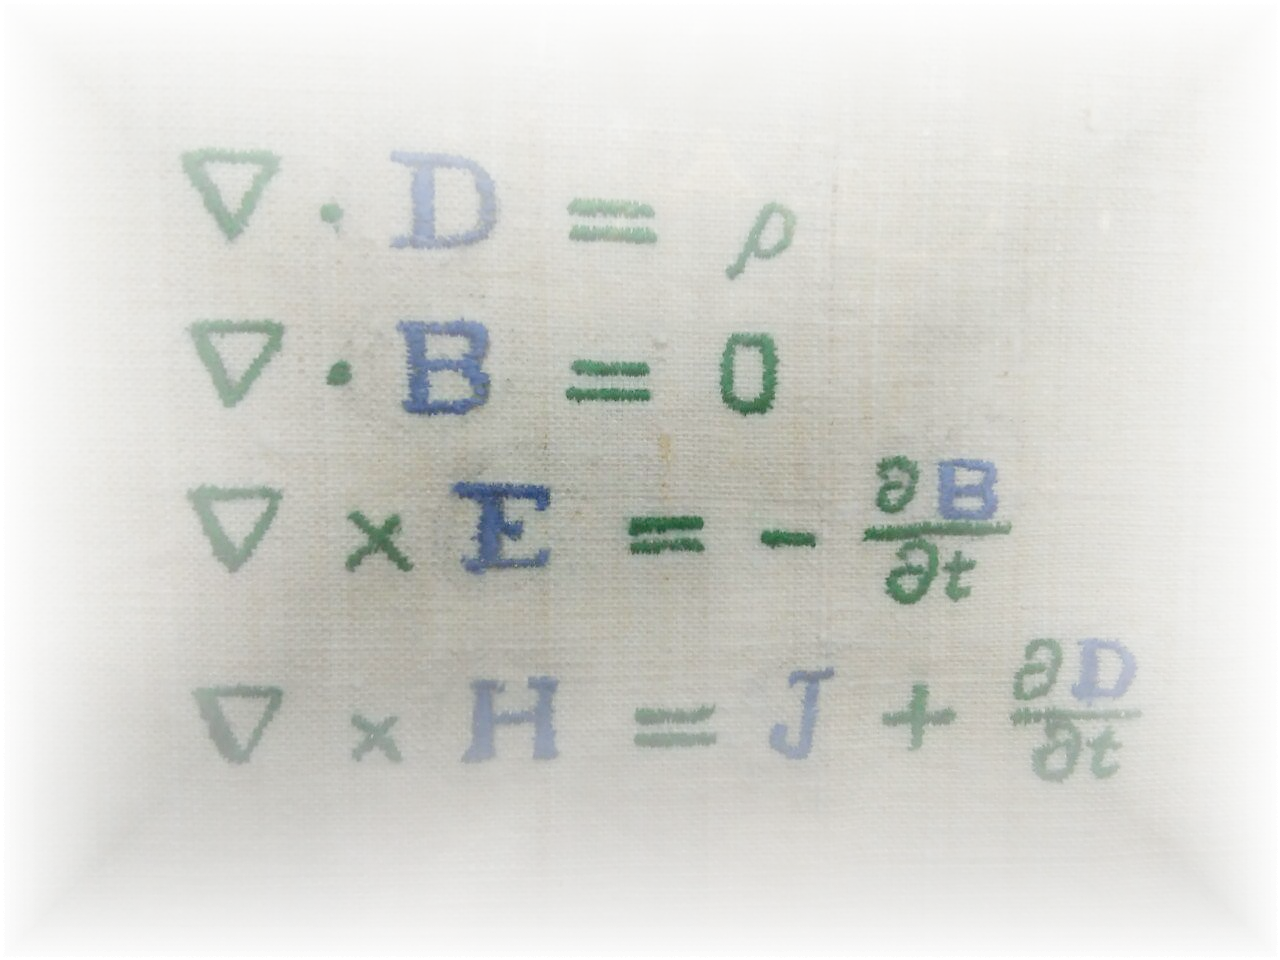
\includegraphics[width=0.6\textwidth]{figures/maxwell.png}
\end{center}

Las ecuaciones homogéneas\footnote{$\nabla \boldrm{D}=0$ y
  $\nabla\times \boldrm{E} + \pdv{\boldrm{B}}{t} = 0$} son fácilmente interpretables como que
$\boldrm{B}$ es el rotacional de un \emph{potencial vector} y
$\boldrm{E}$ un gradiente:
\begin{align}
    \boldrm{B} &= \nabla \times \boldrm{A} \\
  \boldrm{E} &= -\nabla \boldrm{\phi} - \pdv{\boldrm{A}}{t}
\end{align}
Con estas sustituciones podemos reducir las ecuaciones de Maxwell; en el vacío tenemos
\begin{equation}
    \nabla^2 \boldrm{\phi} + \pdv{t} (\nabla \boldrm{A}) =
    \frac{-\rho}{\epsilon_0} 
\end{equation}
y por otra parte\jokenote{Es un ladrillo, naturalmente, como todas las ecuaciones. Pero hay ladrillos bien puestos, veáse la fachada de La Seo.}
\begin{equation}
  \begin{split}
    \nabla^2 \boldrm{A} &= \frac{1}{c^2} \pdv[2]{\boldrm{A}}{t} -
    \nabla \left( \nabla \boldrm{A} + \frac{1}{c^2}
      \pdv{\boldrm{\phi}}{t} \right) = \\
    &= -\mu_0 \boldrm{J}
  \end{split}
  \label{eq:batman}
\end{equation}
Notar que $\nabla^2 \boldrm{A}$ indica tres ecuaciones escalares, no
una. La ventaja de este cambio es que ahora están desacopladas.

Podemos sustituir
\begin{equation}
  \begin{split}
    &\boldrm{A} \ \rightarrow \ \boldrm{A} + \nabla
    \boldrm{\Lambda} \\
    &\boldrm{\phi} \ \rightarrow \ \boldrm{\phi} - \pdv{\boldrm{\Lambda}}{t}
  \end{split}
\end{equation}
y obtenemos los mismos resultados independientemente de la
$\boldrm{\Lambda}(\boldrm{r},t)$\jokenote{Infinitas funciones de este estilo, salvo la función de Diriclhet o alguna parida así.}, a este tipo de transformaciones
se les denomina \emph{transformaciones de gauge}. En particular, para
simplificar la ecuación \eqref{eq:batman}, es interesante escoger el
denominado \emph{gauge de Lorentz}:
\begin{equation}
  - \left( \nabla \boldrm{A} + \frac{1}{c^2}
    \pdv{\boldrm{\phi}}{t} \right) = \nabla^2 \boldrm{\Lambda}
  - \frac{1}{c^2} \pdv[2]{\boldrm{\Lambda}}{t}
\end{equation}
con el que las ecuaciones de Maxwell resultan\footnote{Básicamente,
  con esta elección hacemos que el término $\left( \nabla \boldrm{A} + \frac{1}{c^2}
      \pdv{\boldrm{\phi}}{t} \right)$ de \eqref{eq:batman} sea nulo. }
\begin{equation}
  \begin{split}
    \nabla^2\boldrm{\phi} - \frac{1}{c^2} \pdv[2]{t}
    \boldrm{\phi} &= \frac{-\rho}{\epsilon_0} \\
    \nabla^2 \boldrm{A} - \frac{1}{c^2} \pdv[2]{\boldrm{A}}{t} &=
    -\mu_0 \boldrm{J}
  \end{split}
\end{equation}
de forma que $\boldrm{A}$ se desacopla. La principal ventaja es que es
el mismo para todos los sistemas de referencia. Las fuerzas no cambian
bajo estas transformaciones, ya que dependen de $\boldrm{B}$ y
$\boldrm{E}$, que son invariantes ante estos cambios.
Otra elección es el
\emph{gauge de Coulomb}\jokenote{Habéis estado usando el gauge de
  Coulomb toda la vida. Os hemos estado engañando, pero pasa como con
  los Reyes Magos; mientras dura el engaño se lo pasan muy bien el que engaña y el engañado.}, en que el potencial se propaga de forma
instantánea; si $\boldrm{\phi}=\boldrm{\phi}(t)$ se tiene que
$V\neq V(t)$. Notar que $\boldrm{B},\boldrm{E}$ siguen siendo
  funciones dependientes del tiempo.
Viene de imponer $\nabla \boldrm{A}=0$,
con lo que las ecuaciones quedan
\begin{equation}
  \begin{split}
    \nabla^2 \boldrm{\phi} &= \frac{-\rho}{\epsilon_0} \\
    \nabla^2 \boldrm{A} - \frac{1}{c^2} \pdv[2]{\boldrm{A}}{t} &=
    -\mu_0 \boldrm{J} + \frac{1}{c^2} \nabla \pdv{\boldrm{\phi}}{t}
  \end{split}
  \label{eq:robin}
\end{equation}
El teorema de Helmholtz\footnote{
Wikipedia dixit:
\emph{
Helmholtz's theorem $[\cdots]$ states that any sufficiently smooth, rapidly decaying vector
field in three dimensions can be resolved into the sum of an
irrotational (curl-free) vector field and a solenoidal
(divergence-free) vector field.
}
}\jokenote{Este teorema se llama de nosequién y dice esto} establece en una de sus formas que $\boldrm{J}$ se puede descomponer
en una componente transversal $\boldrm{J}_\perp$ y otra longitudinal
$\boldrm{J}_\parallel$, que verifican $\forall \boldrm{J}$ que  $\nabla
\times \boldrm{J}_\parallel = \boldrm{0}$ y $\nabla \cdot \boldrm{J}=0$.

Con ello y la ecuación de continuidad $\nabla \boldrm{J}+
    \pdv{t}\rho=0$ podemos reescribir las ecuaciones \eqref{eq:robin}
  como\footnote{Utilizamos $\frac{1}{c^2} \nabla
    \pdv{\boldrm{\phi}}{t}=\mu_0 \boldrm{J}_\parallel$, obtenido de
    la ecuacíon de continuidad y de $\nabla^2 \boldrm{\phi} =
    \frac{-\rho}{\epsilon_0}$.} :
  
\begin{equation}
  \begin{split}
    \nabla^2 \boldrm{\phi} &= \frac{-\rho}{\epsilon_0} \\
    \nabla^2 \boldrm{A} - \frac{1}{c^2} \pdv[2]{\boldrm{A}}{t} &=
    -\mu_0 \boldrm{J}_\perp
  \end{split}
  \end{equation}
Vemos que sólo nos importa la componente $\boldrm{J}_\perp$, por ello
al gauge de Coulomb a veces se le denota el \emph{gauge transversal}.
Si $\rho=\abs{\boldrm{J}}=0$ (caso libre) nos queda
  \begin{equation}
  \begin{split}
    \nabla^2 \boldrm{\phi} &= 0\\
    \nabla^2 \boldrm{A} &= \frac{1}{c^2} \pdv[2]{\boldrm{A}}{t} 
  \end{split}
  \end{equation}

\section{Campo electromagnético en el vacío}
Describamos el campo electromagnético de una región del vacío, donde
$\rho=0$ y $\boldrm{J}=0$.\footnote{Evidentemente, fuera de esta
  región de frontera $\rho$ o $\abs{\boldrm{J}}$ no son nulas, ya que
  sino no habría campo alguno.} Utilizaremos el gauge de Coulomb para ello.

Consideremos un campo tal que $\boldrm{\phi}=0$ y $\nabla^2 \boldrm{A}
= \frac{1}{c^2} \pdv[2]{t} \boldrm{A}$. La solución es una
superposición de ondas planas, expresables como
\begin{equation}
  \boldrm{A}_\lambda e^{-i\omega_\lambda t} = L^{-\nicefrac{3}{2}}
  \boldrm{\Pi}_\lambda e^{i \boldrm{k}_\lambda \boldrm{r}} e^{-i
    \omega_\lambda t} 
\end{equation}
donde $\boldrm{\Pi}$ es el vector de polarización y $\omega_\lambda =
\abs{\boldrm{k}_\lambda}c$, con condiciones de normalizacion $\iiint \dd{V}
\abs{\boldrm{A}_\lambda}^2 =1$.

Utilizando que en el gauge de Coulomb $\nabla \boldrm{A} = 0$ y
omitiendo por simplicidad los subíndices $\lambda$, se tiene para
$\hat{x}$
\begin{equation}
  \pdv{A_x}{x} = \pdv{x} \left( \Pi_x e^{i \boldrm{k}
      \boldrm{r}} \right) = \Pi_x (ik_x) e^{i \boldrm{k}\boldrm{r}}
\end{equation}
El cálculo para $\hat{y}, \hat{z}$ es análogo; sumando las tres
derivadas parciales (operador divergecia) se tiene
\begin{equation}
  \nabla \boldrm{A} = i (\Pi_x k_x + \Pi_y k_y + \Pi_z k_z) e^{i \boldrm{k}\boldrm{r}} = 0
  \ \rightarrow \ \boldrm{\Pi} \perp \boldrm{k}
\end{equation}
La solución general para $\boldrm{A}$ es
\begin{equation}
  \boldrm{A}(\boldrm{r},t) = \sum_{\lambda} \left( q_\lambda
    \boldrm{A}_\lambda e^{-i\omega_\lambda t} + q_\lambda^*
    \boldrm{A}_\lambda^* e^{i \omega_\lambda t} \right) \in \mathbb{R}
  \label{eq:aform}
\end{equation}
Es un número real, por lo que $\boldrm{E}$ y $\boldrm{B}$ también lo
son. En particular, para $\boldrm{E}$ se tiene
\begin{equation}
  \boldrm{E} = \frac{1}{c} \pdv{\boldrm{A}}{t} =
 \frac{-i}{c}\sum_{\lambda}  \omega_\lambda\left( q_\lambda
    \boldrm{A}_\lambda e^{-i\omega_\lambda t} - q_\lambda^*
    \boldrm{A}_\lambda^* e^{i \omega_\lambda t} \right) \in \mathbb{R}
\end{equation}
$\boldrm{B}$ se obtiene fácilmente como $\nabla\times \boldrm{A}$.

\subsection{Energía}

La energía del sistema es (en CGS):
\begin{equation}
  E = \frac{1}{8\pi} \iiint_{L^3} \dd{V} \left( \boldrm{E}^2 + \boldrm{B}^2 \right)
\end{equation}

Calculemos los términos. Podemos expresar $\boldrm{E}^2$ como
\begin{equation}
  \boldrm{E}^2 =  \frac{1}{c^2} \left( \sum_{\lambda} \cdots \right) \left( \sum_{\lambda'} \cdots \right)
\end{equation}

Comenzamos por los términos directos, en los que $\lambda=\lambda'$.

\begin{equation}
  \frac{-\omega}{c^2} \left( q^2 \boldrm{A} \boldrm{A}
    e^{-2i\omega t} + q^{*2} \boldrm{A}^*  \boldrm{A}^*
    e^{2i\omega t} - qq^* \boldrm{A}\boldrm{A}^* - q^*q \boldrm{A}^* \boldrm{A} \right)
\end{equation}
Recordando que $\boldrm{A}=L^{-\nicefrac{3}{2}} \boldrm{\Pi} e^{i
  \boldrm{k}\boldrm{r}}$ vemos que $\boldrm{A}\boldrm{A}^* = L^{-3}
\underbrace{\abs{\Pi}^2}_{=1} = \boldrm{A}^* \boldrm{A}$, y que
$\boldrm{A}\boldrm{A} = L^{-3} \abs{\boldrm{P}}^2 e^{2 i
  \boldrm{k}\boldrm{r}}$. La integral de $\boldrm{A}\boldrm{A}$
quedará como
\begin{equation}
  \iiint_{L^3} \dd{V} \boldrm{A} \boldrm{A} = \int_0^L \dd{x} e^{2i
    k_x x} \int_0^L \dd{y} e^{2i
    k_x y}  \int_0^L \dd{z} e^{2i
    k_x z}
\end{equation}
donde los términos son nulos por las condiciones de
contorno\footnote{En cada integral se obtiene $\eval{\frac{1}{2ik_x}
    \exp(i2k_xx)}_0^L$, pero las condiciones de contorno periódicas
  anulan estos términos (valen lo mismo en $0$ y en $L$).}.

Para los términos cruzados $\lambda\neq\lambda'$ se obtiene
\begin{equation}
  \begin{split}
    \frac{-\omega\omega'}{c} \Big[& qq' \boldrm{A}\boldrm{A}'
    e^{-i(\omega+\omega')t} + q^* q'^{*} \boldrm{A}^*
    \boldrm{A}'^{*} e^{i(\omega+\omega')t} -\\
    &- q q'^* \boldrm{A} \boldrm{A}^{*} e^{-i(\omega-\omega')t} - q^*
    q' \boldrm{A}^* \boldrm{A}' e^{i(\omega-\omega')t} \Big]
  \end{split}
\end{equation}

Por las mismas razones que antes, las integrales $\iiint
\boldrm{A}\boldrm{A}$ se cancelan.

Las integrales finales quedan
\begin{equation}
  \iiint_{L^3} \frac{1}{8\pi} \boldrm{E}^2 \dd{V} = \iiint_{L^3}
  \frac{1}{8\pi}\boldrm{B}^2 \dd{V} = \frac{\omega^2}{c^2} (q^* q + q ^*)
\end{equation}
y obtenemos que la energía es
\begin{equation}
  E = \frac{1}{4\pi c^2} \sum_{\lambda} \omega_\lambda^2 q_\lambda^* q_\lambda
\end{equation}
Definimos las nuevas variables ``posición'' y ``momento'', por
analogía\footnote{Se omite la demostración}:
\begin{align}
 Q_\lambda &= \frac{1}{\sqrt{4\pi c^2}}
(q^*_\lambda + q_\lambda) \\
P_\lambda &= \frac{i\omega_\lambda}{\sqrt{4\pi c^2}}
(q^*_\lambda - q_\lambda)
\end{align}
Obtenemos un hamiltoniano similar al de un
oscilador armónico:
\begin{equation}
  \Ham = \sum_{ \lambda} \frac{1}{2} \left( P_\lambda^2 +
    \omega_\lambda^2 Q_\lambda^2  \right)
  \label{eq:oscilatorem}
\end{equation}
\subsection{Cuantificación}
Vemos en \eqref{eq:oscilatorem} que el campo electromagnético se puede modelar como un conjunto
de osciladores armónicos independientes. La energía es simplemente la
suma de las energías de cada ``oscilador'' (figura \ref{fig:muellefotonico}):
\begin{equation}
  E = \sum_{ \lambda} \left( n_\lambda + \frac{1}{2} \right) \hbar\omega_\lambda
\end{equation}
\begin{marginfigure}
  \begin{tikzpicture}
    \tikzstyle{boing}=[snake=coil, line after snake=0.1cm
    , line before snake = 0.1cm
    , segment amplitude = 0.15cm]
    % Draw the balls
    \node[circle,fill=blue,inner sep=2.5mm] (a) at (1.5,4) {};
    \node[circle,fill=blue,inner sep=2.5mm] (b) at (3,3) {};
    \node[circle,fill=blue,inner sep=2.5mm] (c) at (2,2) {};
    % Draw the springs
    \draw[boing, segment length = 0.5mm] (0.5,4) to (a);
    \draw[boing, segment length = 2mm] (0.5,3) to (b);
    \draw[boing, segment length = 1mm] (0.5,2) to (c);
    % Labels
    \node[right] (a) at (3.5,3) {$x_2,m_2,k_2$};
    \node[right] (a) at (2,4) {$x_1,m_1,k_1$};
    \node[right] (a) at (2.5,2) {$x_3,m_3,k_3$};
    % Wall
    \fill [color=black!20] (0.2,1) rectangle (0.5,5);
    \draw[ultra thick] (0.5,1) -- (0.5,5);
  \end{tikzpicture}
  \caption{Modelizado del campo EM como un conjunto de osciladores}
  \label{fig:muellefotonico}
\end{marginfigure}
con autoestados $\ket{n_{\lambda1}} \otimes \ket{n_{\lambda2}} \otimes
\cdots$ que dan cuenta de los \emph{números de ocupación} o número de
fotones de cada $\lambda_i$.\footnote{Se suelen escribir como 
  \begin{equation*}
    \ket{n_{\lambda1},n_{\lambda2},n_{\lambda3},\cdots}
  \end{equation*}
}

Definimos los operadores de creación y destrucción:
\begin{align}
  a_\lambda^\dagger &= \frac{1}{\sqrt{2 \hbar\omega_\lambda}}
  (\omega_\lambda Q_\lambda - i P_\lambda) =
                      \sqrt{\frac{\omega_\lambda}{2\pi \hbar c^2}} q_\lambda^*\\
  a_\lambda&= \frac{1}{\sqrt{2 \hbar\omega_\lambda}}
  (\omega_\lambda Q_\lambda + i P_\lambda) =
                      \sqrt{\frac{\omega_\lambda}{2\pi \hbar c^2}} q_\lambda
\end{align}
Es inmediato que $[a^\dagger,a]=1$. Además,
$[a_\lambda,a_{\lambda'}^\dagger]=0$ al actuar en espacios distintos.

El efecto de los operadores de creación y destrucción es
idéntico al
del caso del oscilador armónico:
\begin{align}
  a_\lambda^\dagger \ket{\cdots,n_\lambda,\cdots} &=
                                                    \sqrt{n_\lambda+1}\ket{\cdots,n_\lambda+1,\cdots} \\
  a_\lambda \ket{\cdots,n_\lambda,\cdots} &= \sqrt{n_\lambda}\ket{\cdots,n_\lambda-1,\cdots}
\end{align}
Hay que recordar que hay que extender los operadores con la
  identidad. Por ejemplo,\[a_3 \coloneqq \mathbb{I}\otimes 
    \mathbb{I}\otimes a_3\otimes  \mathbb{I} \otimes \cdots \]

De igual forma, podemos definir el operador número $N$ como $N_\lambda
= a_\lambda^\dagger a_\lambda$, obteniendo
\begin{equation}
  \Ham = \sum_{\lambda} \hbar \omega_\lambda \left( N_\lambda + \frac{1}{2} \right)
\end{equation}
El inconveniente de esta formulación es que la energía del vacío,
$\ev{\Ham}{0}$, es infinita\footnote{Esto es debido a que los kets
  tienen infinitos elementos, y el sumatorio corre sobre infinitos
  términos.}. Resolvemos este problema con la siguiente
renormalización:
\begin{equation}
  \Ham = \sum_{\lambda} \hbar\omega N_\lambda
\end{equation}
de forma que $\ev{\Ham}{0}=0$.

\section{Interacción del campo EM con la materia}
Consideramos el campo EM creado por cargas al moverse, y como influye
en su movimiento; el sistema típico a estudio es el átomo. Utilizamos
como sistema de referencia inercial el núcleo, por su escaso
movimiento, y escribimos el hamiltoniano\footnote{Es un hamiltoniano
  propuesto por Fermi, en sistema CGS y con el gauge de Coulomb. En \emph{Mecanique quantique}, de Claude Cohen-Tannoudji, hay una explicación exhaustiva de la elección.} del sistema:
\begin{equation}
  \Ham = \frac{1}{2m} \left( \boldrm{p}_i - \frac{e_i}{c}
    \boldrm{A}_\perp (\boldrm{r}_i) \right)^2 + \sum_{i<j}
  \frac{e_ie_j}{\abs{\boldrm{r}_i - \boldrm{r}_j}} + \Ham_\text{EM}(\boldrm{A}_\perp)
  \label{eq:hamiltonrules}
\end{equation}
Notar que no es un hamiltoniano de partículas independientes. 

Si consideramos una sola carga y las ecuaciones de Hamilton\footnote{
  \begin{align*}
    \dot{p} &= \pdv{\Ham}{q}\\
    \dot{q} &= \frac{-\partial \Ham}{\partial p}
  \end{align*}
} obtenemos la fuerza de Lorentz. El desarrollo concreto puede
consultarse en \emph{Mecanique quantique}, de Claude Cohen-Tannoudji.

Consideremos un átomo, en el que $e_i=-e$ y $m_i=m$, con la masa del
núcleo aproximable a infinita. El hamiltoniano \eqref{eq:hamiltonrules} queda como
\begin{equation}
  \begin{split}
  \Ham &= 
  \textcolor{red!60!black}{
  \sum_{i=1}^N \frac{p_i^2}{2m} + V 
  }
  + \\
  &+ 
  \textcolor{blue!60!black}{
  \frac{e}{2mc} \sum_{i=1}^N \left[ \boldrm{p}_i
    \boldrm{A}(\boldrm{r}_i,t) + \boldrm{A}(\boldrm{r}_i,t) \boldrm{p}_i \right]+
    \frac{e^2}{2mc^2} \sum_{i=1}^N \boldrm{A}^2(\boldrm{r}_i,t)
    }
  + \\
    &+
    \textcolor{green!60!black}{
 \Ham_\text{EM}
 }
  \end{split}
  \label{eq:aynomames}
\end{equation}
Por lo que tenemos $\Ham = 
 \textcolor{red!60!black}{\Ham_\text{at.}}
+\textcolor{blue!60!black}{\Ham_\text{int}}
+\textcolor{green!60!black}{\Ham_\text{EM}}$. Definimos $\Ham_0 =
\Ham_\text{at.}+\Ham_\text{EM}$, de forma que $\Ham =
\Ham_0+\Ham_\text{int}(t)$. Notar que falta el término de interacción
con el espín\footnote[][-3cm]{Sería un término extra de la
  forma \[\sum_{i}-\boldrm{\mu}_i(\boldrm{\Pi}\times \boldrm{A})\]No
  es necesario incluirlo ya que cortaremos la aproximación en primer
  orden (dipolo eléctrico) y ahí no entra el término de espín.}.

\subsection{Aproximación perturbativa de la emisión espontánea}
La probabilidad de que en el átomo se produzca una emisión espontánea
de un fotón viene dada por
\begin{equation}
  P_{if}(t) = \frac{1}{\hbar^2} \abs{\int_0^t
    \mel{\phi_f}{\Ham_\text{int}(\tau)}{\phi_i} e^{i\omega_{fi}\tau}\dd{\tau} }^2 
  \label{eq:probaif}
\end{equation}
Caracterizamos al estado inicial $\phi_i$ como $\ket{I}$ y al final
$\phi_f$ como $\ket{F}$ para aliviar la notación. En función de sus
valores, tenemos distintos fenómenos físicos:
\marginnote{Para aliviar la notación, se empleará a partir de ahora
  $\ket{\cdots,a,\cdots}\equiv\ket{a}$,
  $\ket{\cdots,a,b,\cdots}\equiv\ket{a,b}$, etc. Se sobreentienden las
componentes no nombradas del autoestado.} 
\begin{itemize}
\item Si $\ket{I}=\ket{1_\lambda}$ y
  $\ket{F}=\ket{0_\lambda}$, se ha absorbido un fotón.
\item Si en cambio $\ket{F}=\ket{1_\lambda}$ y
  $\ket{I}=\ket{0_\lambda}$, estamos ante la emisión
  espontánea de un fotón por el átomo.
\item Para $\ket{I}=\ket{1_\lambda}$, si se tiene
  emisión inducida por el fotón $1_\lambda$ se obtendrá
  $\ket{F}=\ket{2_\lambda}$ (se excita un fotón de
  idéntica longitud de onda) o
  $\ket{F}=\ket{1_\lambda,1_{\lambda'}}$ (el fotón
  excitado es de distinta $\lambda$).
\end{itemize}

Para calcular la integral \eqref{eq:aynomames} necesitamos ver si
$\boldrm{A}$ y $\boldrm{p}$ conmutan:
\begin{equation}
  \begin{split}
    (\boldrm{p}\boldrm{A}) \boldrm{\phi} &= -i \hbar \nabla (\boldrm{A}\boldrm{\phi}) =
    \\
    &= \left( \pdv{x} A_x\boldrm{\phi} +  \pdv{y} A_y\boldrm{\phi}+ \pdv{z} A_z\boldrm{\phi}
    \right) =\\
    &= -i \hbar \left[ (\nabla \boldrm{A})\boldrm{\phi}+ \boldrm{A}\nabla \boldrm{\phi}
    \right] = \\
    &= (\boldrm{A}\boldrm{p})\boldrm{\phi} 
  \end{split}
\end{equation}

De donde de vemos que el término
$\boldrm{p}\boldrm{A}+\boldrm{A}\boldrm{p}$ de \eqref{eq:aynomames} es
simplemente $2 \boldrm{A}\boldrm{p}$. Utilizando la ecuación
\eqref{eq:aform} para $\boldrm{A}$ vemos que el primer sumando de $\Ham_\text{int}$ 
puede escribirse como
\begin{equation}
  \begin{split}
    \frac{e}{2mc} \sum_{i} \left[ \boldrm{p}_i \boldrm{A} +
      \boldrm{A}\boldrm{p} \right] &= 2\cdot\frac{e}{2mc} \sum_{i} \sum_{\lambda} \Big[
    \mel{F}{\boldrm{A}_{\lambda'}\boldrm{p}_i e^{-i\omega'_\lambda
        t}}{I} \mel{n_\lambda = 1}{q_{\lambda'}}{0} +  \\
    &+
\mel{F}{\boldrm{A}_{\lambda'}^*\boldrm{p}_i e^{i\omega'_\lambda
        t}}{I} \mel{n_\lambda = 1}{q_{\lambda'}^\dagger}{0} \Big]= \cdots
  \end{split}
\end{equation}
donde estamos suponiendo situación de emisión espontánea. El término
$\mel{n_\lambda=1}{q_\lambda'}{0}$ se anula, ya que se aplica el
operador destrucción al vacío, $\ket{0}$. El segundo término se puede
reescribir en función del operador creación utilizando que $q_{\lambda'}^\dagger\ket{0} = \left(
  \frac{2\pi \hbar c^2}{\omega_{\lambda'}}
\right)^2\cdot1\ket{n_{\lambda'}=1}$. De esta forma, nos quedan
términos
$\ket{n_\lambda=1}{n_{\lambda'}=1}=\delta_{\lambda,\lambda'}$, que
eliminan todos los $\lambda'$ del sumatorio excepto $\lambda$:

\begin{equation}
  \begin{split}
    \cdots &= \sum_{i} \frac{e}{mc} \sqrt{ \frac{2\pi \hbar
        c^2}{\omega_\lambda} }  
\mel{F}{\boldrm{A}_{\lambda'}^*\boldrm{p}_i }{I} e^{i\omega'_\lambda
        t}
  \end{split}
\end{equation}

Para el otro término de $\Ham_\text{int}$, que depende de
$\boldrm{A}^2$, tenemos un doble sumatorio (uno por cada
$\boldrm{A}$). No obstante, vemos que es nulo al aparecer varios
braket $\braket{I}{F}=\braket{1_\lambda}{0}$:
\begin{itemize}
\item Los elementos $q_{\lambda'}q_{\lambda''}\ket{0}$ son nulos al
  aplicarse el operador destrucción al vacío.
\item Para los términos creación-destrucción se tiene
\begin{equation}
  \mel{1_\lambda}{q_{\lambda'}q^\dagger_{\lambda''}}{0} \sim
  \braket{1_\lambda}{1_{\lambda'}1_{\lambda''}} = 0
\end{equation}
que se anula porque los osciladores son independientes.
\item El término
  $\mel{1_\lambda}{q_{\lambda'}q_{\lambda''}^\dagger}{0} \sim
  \mel{1_{\lambda'}}{q_{\lambda'}}{1_{\lambda''}}$ puede actuar sobre
  una coordenada no vacía ($\braket{1_\lambda}{0}=0$) o sobre una
  coordenada vacía, en cuyo caso resulta nulo al estar aplicándose $q$ a $\ket{0}$.
\end{itemize}

Con todo lo visto, la probabilidad \eqref{eq:probaif} de emisión
espontánea queda
\begin{equation}
  P_{if} = \frac{1}{\hbar^2} \frac{e^2}{m^2c^2} \left( \frac{2\pi
      \hbar c^2}{\omega_\lambda} \right) \abs{\mel{F}{\textstyle \sum \displaystyle
      \boldrm{A}_\lambda^*(\boldrm{r}_i)\boldrm{p}_i}{I}}^2
  \abs{F(\omega_{fi}+\omega_\lambda,t)}^2
  \label{eq:machete}
\end{equation}
donde 
\begin{equation}
F(\omega_{fi}+\omega_\lambda,t) = \int_0^t
e^{i(\omega_{fi}+\omega_\lambda)t'} = \left[ \frac{\sin[(\omega_{fi}+\omega_\lambda)\frac{t}{2}]}{\frac{1}{2}(\omega_{fi}+\omega_\lambda)} \right]^2
\end{equation}
$F$ tiene un límite asintótico en $t\to\infty$ dado por
$\lim_{t\to\infty}\frac{\sin^2\alpha t}{\alpha^2}=\pi t \cdot
\delta(\alpha)$. Sustituyendo este resultado y diviendo entre $t$ la
ecuación \eqref{eq:machete} hallamos la probabilidad de transición por
unidad de tiempo $\Lambda_{fi}$:
\begin{equation}
  \Lambda_{fi} = \frac{2\pi}{\hbar} \abs{H_{fi}}^2 \delta(E_{fi}+E_\lambda)
\end{equation}
con dimensiones de inversa de
tiempo\footnote{$[\delta(E_{fi}+E_\lambda)]=E^{-1}$. Puede verse en
  ejemplos como $\int_{\mathbb{R}}\delta(x)\dd{x}=1$}. Notar que la
delta de Dirac refleja un resultado ya conocido, que la energía del
fotón tiene que coincidir con la $\Delta E$ entre niveles para que se
efectúe una transición.

El fotón tiene un momento $\boldrm{k}_\lambda$ dentro de un continuo;
la probabilidad de encontrar uno con un momento exacto es nula.
Queremos calcular sumas del estilo $\sum_{f}\Lambda_{if}$ para ver la
probabilidad de transición total de un nivel dado, para ello
recurrimos a calcular la \emph{densidad de estados}, transformándose
la suma en una integral.
Se utilizan condiciones de contorno periódicas en
el borde de cada cubo del $k$-espacio ($e^{ik_x0}=e^{ik_xL}=1$), de forma que
\begin{equation}
  k_{x_i} = n_{x_i} \frac{2\pi}{L}; \ \ n_{x_i} \in \{\pm1,\pm2,\cdots\}
\end{equation}
donde $x_i \in \{x,y,z\}$. De esta forma, quedan definidos sucesivos
nodos cúbicos separados $\frac{2\pi}{L}$ en los ejes, correspondiendo
cada nodo a una $\boldrm{k}$ (figura \ref{fig:nodoloco}).


\begin{marginfigure}
  \begin{tikzpicture}[xscale=1,yscale=1]
    % y axis
    \draw [thick,gray] (0,0) -- (2,0);
    \draw [gray,fill] (0,0) circle (0.05);
    \draw [gray,fill] (1,0) circle (0.05);
    \draw [gray,fill] (2,0) circle (0.05);
    \draw node [right] at (2.1,0) {$k_y$};
    % z axis
    \draw [thick,gray] (0,0) -- (0,2);
    \draw [gray,fill] (0,0) circle (0.05);
    \draw [gray,fill] (0,1) circle (0.05);
    \draw [gray,fill] (0,2) circle (0.05);
    \draw node [above] at (0,2.1) {$k_z$};
    % x axis
    \draw [thick,gray] (0,0) -- (-1,-1);
    \draw [gray,fill] (0,0) circle (0.05);
    \draw [gray,fill] (-0.5,-0.5) circle (0.05);
    \draw [gray,fill] (-1,-1) circle (0.05);
    \draw node [below left] at (-1,-1) {$k_x$};
    % cube bottom
    \draw [thick, black]
     (0,0) -- (1,0) -- (0.5,-0.5) -- (-0.5,-0.5) -- (0,0);
    % cube top
    \draw [thick, black]
     (0,1) -- (1,1) -- (0.5,+0.5) -- (-0.5,+0.5) -- (0,1);
    % cube walls
     \draw [thick,black] (0,0) -- (0,1);
     \draw [thick,black] (1,0) -- (1,1);
     \draw [thick,black] (-0.5,-0.5) -- (-0.5,0.5);
     \draw [thick,black] (+0.5,-0.5) -- (+0.5,0.5);
    % some labels
     \draw [thin,blue, <->] (1,-0.2) -- (2,-0.2);
    \draw node [below,blue] at (1.5,-0.2) {$\frac{2\pi}{L}$};
  \end{tikzpicture}
  \caption{$k$-espacio de integración. Se muestra un nodo cúbico
    correspondiente a una $\boldrm{k}$.}
  \label{fig:nodoloco}
\end{marginfigure}

Un diferencial de volumen del $k$-espacio correspondrá a
$\frac{k^2}{(2\pi/L)^3}\dd{k}\dd{\Omega}$ nodos
$\boldrm{k}$\footnote{Se ha efectuado un cambio a coordenadas polares;
$k^2 \dd{k} \dd{\Omega}$ es equivalente al típico $\dd{V}=r^2 \dd{r} \sin{\theta}\dd{\theta}$.};
relacionando $\abs{\boldrm{k}}$ con la energía se tiene
\begin{equation}
  E = \hbar c k = \left( \frac{L}{2\pi} \right)^3 \frac{E^2}{(\hbar
    c)^3} \dd{E} \dd{\Omega}
\end{equation}
Calculamos la densidad de estados como $\rho(E) = E/\dd{E}$:
\begin{equation}
  \rho(E_\lambda) = \left( \frac{L}{2\pi} \right)^3 \frac{E^2}{(\hbar
    c)^3} \dd{\Omega}
\end{equation}

Ahora, ya estamos en condiciones de calcular la suma:
\begin{equation}
  \begin{split}
    \sum_{f} \Lambda_{if} &= \int_\star \dd{E_\lambda}
    \frac{2\pi}{\hbar} \abs{\Ham_{fi}}^2 \delta(E_{fi}+E_\lambda)
    \rho(E_\lambda) =\\
    &= \frac{2\pi}{\hbar}\abs{\Ham_{fi}}^2 \rho(E_\lambda)
  \end{split}
\end{equation}

Donde $\rho(E_\lambda) = \rho(E_{fi})$. La región de integración
abarca el rango de la instrumentación utilizada, por ejemplo de
\SI{300}{\nano\metre} a \SI{600}{\nano\metre} y un ángulo sólido
correspondiente a media esfera. 




\subsection{Aproximación dipolar eléctrica}
\marginnote{Seguimos considerando emisión espontánea}Para poder aplicar esta aproximación se ha de cumplir que
$\lambda=\frac{2\pi}{k_\lambda}$ sea muy inferior al tamaño del átomo,
verificándose en tal caso que en sus vecindades $e^{-i
  \boldrm{k}\boldrm{r}}\simeq 1$.

Veamos el valor de la contribución
$\mel{F;n_\lambda=1}{-\boldrm{\mu}_s (\nabla\times \boldrm{A})}{I}$ del espín al hamiltoniano, antes
despreciado:
\begin{equation}
  \nabla\times \boldrm{A} = i \sum_{\lambda} \boldrm{k}_\lambda\times
  (q_\lambda \boldrm{A}_\lambda e^{-i\omega_\lambda t} +
  q_\lambda^\dagger \boldrm{A}_\lambda^* e^{i\omega_\lambda t})
\end{equation}
El primer término del producto vectorial aplicado en el elemento de
matriz del espín será del estilo $q\ket{I}=q\ket{0}$, siendo por
tanto nulo. El segundo nos dará un braket
$\braket{n_\lambda}{n_{\lambda'}} \sim \delta_{\lambda,\lambda'}$, eliminando todos los términos del
sumatorio salvo uno. Obtenemos:
\begin{equation}
  \mel{F}{-\boldrm{\mu}_s e^{i \boldrm{k}_\lambda \boldrm{r}_i } (i
    \boldrm{k}_\lambda \times \boldrm{\Pi}_\lambda) e^{i
      \omega_\lambda t}}{I}
\end{equation}
Expresando el momento magnético en función del
espín\footnote{$\boldrm{\mu}_s = g_s \mu_{\scriptstyle B}
  \frac{\boldrm{s}}{\hbar}\simeq 2 \mu_{\scriptstyle B}
  \frac{\boldrm{s}}{\hbar} = \frac{e}{mc} \boldrm{s}$} obtenemos
\begin{equation}
  \mel{F}{
    \sum_{i} \boldrm{S}_i (\boldrm{k}_\lambda \times
    \boldrm{\Pi}_\lambda) \underbrace{e^{-i \boldrm{k}_\lambda
        \boldrm{r}_i}}_{\simeq 1}
}{I}
\end{equation}
Se puede comparar con el elemento del dipolo eléctrico y ver que es
claramente inferior:
\begin{equation}
  \frac{\mel{F}{\boldrm{\Pi}_\lambda
      \boldrm{p}_i}{I}}{\mel{F}{\boldrm{s}_i (\boldrm{k}_\lambda
      \times \boldrm{\Pi}_\lambda)}{I}} = \frac{mv
    \frac{R}{R}}{\frac{\hbar}{2} \frac{1}{\lambda}} \sim \frac{\hbar
    \frac{1}{R}}{\hbar \frac{1}{\lambda}} \sim \frac{\lambda}{R} \gg 1
\end{equation}

Por tanto utilizaremos el hamiltoniano
\begin{equation}
  \Ham_{at.} = \sum_{i} \frac{p_i^2}{2m} + \sum_{i} \frac{Ze^2}{r_i} +
  \sum_{i<j} \frac{e^2}{r_{ij}}
\end{equation}
Calculamos el conmutador de $x_i$ con $\Ham_\text{at.}$:
\begin{equation}
  \begin{split}
    [x_i,\Ham_\text{at.}] &= \frac{1}{2m} [x_i,p_i^2] =
    \frac{1}{2m}[x_i,p_{ix}^2] = \\
    &= \frac{1}{2m} ([x_i,p_{ix}]p_{ix}+p_{ix}[x_i,p_ix]) = \frac{2i
      \hbar p_{ix}}{2m}
  \end{split}
\end{equation}
donde se ha utilizado que $[x_i,p_{ix}]=i \hbar$. Obtenemos:
\begin{equation}
  [\boldrm{r}_i,\Ham_\text{at.}] = i \hbar \frac{\boldrm{p}_i}{m}
\end{equation}
y por lo tanto $\boldrm{p}_i =
\frac{im}{\hbar}[\Ham_\text{at.},\boldrm{r}_i]$. Introduciendo esto en
el elemento de matriz, obtenemos la probabilidad de emisión espontánea
de un fotón, que está notablemente simplificada respecto a \eqref{eq:machete}:
\begin{equation}
 \Lambda_{if} = \frac{e^2}{2\pi \hbar}
 \underbrace{\frac{E_\lambda^2}{(\hbar c)^3 }E_\lambda}_{k^3}
 \abs{\mel{F}{\boldrm{\Pi}_\lambda \textstyle \sum_i \displaystyle
     \boldrm{r}_i}{I}}^2 \dd{\Omega}
\end{equation}
Es inmediato ver que $\mel{F}{\boldrm{\Pi}\boldrm{R}}{I} =
\boldrm{\Pi}\mel{F}{\boldrm{R}}{I}$,donde $\boldrm{R}_i =
\sum_{i}\boldrm{r}_i$. Con esto, obtenemos
\begin{equation}
  \Lambda_{if} = \frac{e^2}{2\pi \hbar} k^3
  \abs{\mel{F}{\boldrm{R}}{I}\cdot \boldrm{\Pi}}^2 \dd{\Omega}
\end{equation}
\marginnote[-2cm]{A partir de ahora se omitirán los subíndices $\lambda$,
  sobreentendiéndose.}

Los fotones emitidos tienen una polarización $\boldrm{\Pi}$ en un
diferencial de ángulo sólido $\dd{\Omega}$. Como el elemento de matriz
puede ser complejo, se puede definir como
\begin{equation}
  \mel{F}{\boldrm{R}}{I} = \boldrm{R}' + i \boldrm{R}''
\end{equation}
con $\boldrm{R}',\boldrm{R}''\in \mathbb{R}^3$. Podemos pintar estos dos vectores en un triedro (figura \ref{fig:triedro}).
\begin{marginfigure}
  \centering
  \vspace{2cm}
  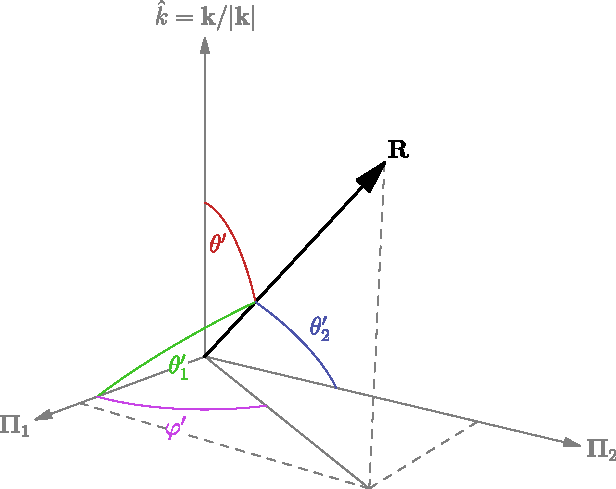
\includegraphics[width=\textwidth]{figures/triedro.pdf}
  \caption{Triedro de la parte real del elemento de matriz del campo
    EM. El elemento imaginario es similar; ponemos
  dos tildes a sus coordenadas para identificarlas en lugar de una sola.}
  \label{fig:triedro}
\end{marginfigure}
El ángulo que forma $\boldrm{R}'$ con una polarización $\boldrm{\Pi}_i$ será del
estilo $\boldrm{R}'\cdot \boldrm{\Pi}_i =
\cos(\theta'_i)|\boldrm{R}'|$, de forma que obtenemos para las dos
polarizaciones ortogonales posibles
\begin{align}
  \cos(\theta'_1) &= \sin(\theta')\cos(\varphi')
  \label{eq:mini1} \\
  \cos(\theta'_2) &= \sin(\theta')\sin(\varphi')
  \label{eq:mini2}
\end{align}
Para $\boldrm{R}''$ obtenemos lo mismo pero con dos tildes \verb~'~ en lugar de una.
Supuesta polarización en $\boldrm{\Pi}_1$,
\begin{equation}
  \Lambda_{if} = \frac{e^2}{2\pi \hbar}k^3 (\abs{\boldrm{R}'}^2
  \cos^2\theta'_1 + \abs{\boldrm{R}''}^2
  \cos^2\theta''_1) \dd{\Omega}
\end{equation}
Suponiendo que no estamos interesados en medir la polarización, sólo
tenemos que sumar ambas intensidades. Hay una suma de cosenos, que
resolvemos mediante identidades trigonométricas\footnote{Sumando la
  ecuación \eqref{eq:mini1} al cuadrado con la ecuación
  \eqref{eq:mini2} al cuadrado obtenemos \[\cos^2\theta'_1+\cos^2\theta'_2=\sin^2\theta'\]}:
\begin{equation}
  \Lambda_{if} = \frac{e^2}{2\pi \hbar} (\abs{\boldrm{R}'}^2
  \sin^2\theta' + \abs{\boldrm{R}''}^2
  \sin^2\theta''  ) \dd{\Omega}
\end{equation}
\subsection{Vida media}
El siguiente paso es integrar $\Lambda_{if}$ a todo el espacio;
ponemos un detector que ocupe todo el ángulo sólido. Utilizamos que
\begin{equation}
  \int_{4\pi} \dd{\Omega} \sin^2\theta \sin \theta \dd{\Omega} = \frac{8\pi}{3}
\end{equation}
y obtenemos ($\boldrm{R}=\hat{z}$):
\begin{equation}
  \boxed{
  \Lambda_{if} (\text{CGS}) = \frac{4e^2}{3 \hbar} k^3 \abs{\mel{F}{\boldrm{R}}{I}}^2
  }
\end{equation}
No hay que perder de vista que estamos calculando la probabilidad de
caída de un fotón desde un nivel $I$ a un nivel $F$ (figura
\ref{fig:caida}). La ecuación está en CGS, en sistema internacional
requiere un factor $\frac{1}{4\pi \varepsilon_0}$.
\begin{marginfigure}
  \begin{tikzpicture}[xscale=2,yscale=1.5]
    % levels
    \draw [ultra thick,blue] (0,0) -- (1.5,0);
    \draw [ultra thick,blue] (0,1) -- (1.5,1);
    \draw node [right] at (1.5,0) {$I$};
    \draw node [right] at (1.5,1) {$F$};
    % photon
    \draw [thick,yellow!94!black,
    snake=snake,
    line after snake=0.2cm, ->] (0.6,0.5) -- (1.5,0.5);
    % Decay line
    \draw [thick, <-] (0.5,0.1) -- (0.5,0.9);
  \end{tikzpicture}
  \caption{Qué demonios estamos haciendo}
  \label{fig:caida}
\end{marginfigure}
Podemos calcular la variación en la población de $I$ con $\text{d}N_i
= -\Lambda N_i \dd{t}$, obteniendo que
\begin{equation}
  N_i(t) = N_i(0) e^{-\Lambda t}
\end{equation}
Obtenemos el parámetro \emph{vida media},
$\tau=\nicefrac{1}{\Lambda}$, que es tanto medible como calculable,
por lo que es \underline{\emph{comparable}}\jokenote{(golpea la
  pizarra)}.

\section{Reglas de selección}
Las reglas de selección\jokenote{Penúltimo esfuerzo agónico} (aquí estudiadas en transiciones dipolares eléctricas)
indican bajo qué condiciones el elemento de matriz
$\mel{F}{\boldrm{R}}{I}$ se anula. 
\jokemargin{Tierra a los ojos}

Tras el estudio de las reglas de recurrencia de los coeficientes de
Clebsch-Gordan, puede verse un sistema homogéneo equivalente en los
\emph{operadores tensioriales}:

\begin{mydef*}[Operador tensorial]
  Se definen\jokenote{Y esta mierda de definición, ¿para qué? Porque damos vueltas como peonzas alrededor de gilipolleces} los \emph{operadores tensoriales bajo $\boldrm{J}$} como
  $2k+1$ operadores $T_q^k$ que cumplen las relaciones:
  \begin{align}
    [J_z,T_q^k] &= \hbar q T_q^k \label{eq:firstsausage}\\
    [J_{\pm},T_q^k] &=  \hbar \sqrt{k(k+1)-q(q\pm1)} T_{q\pm1}^k \label{eq:secondsausage}
  \end{align}
  con $k\in \mathbb{Z}^+$ y $q \in \{-k,\cdots,k\}$.
\end{mydef*}

Físicamente se corresponden con los multipolos electromagnéticos.
Presentan las siguientes propiedades:
\begin{enumerate}
\item De \eqref{eq:firstsausage} deducimos que
$\mel{\alpha'j'm'}{T_q^k}{\alpha jm}=0$ si $m'\neq q+m$. 
\item Viendo \eqref{eq:secondsausage} empleamos la notación
\begin{equation}
  \begin{split}
    \mel{\alpha'j'm'}{[J_\pm,T_q^k]}{\alpha j m}  \to  \mel{\alpha'JM}{[J_\pm,T_{m_2}^{J_2}]}{\alpha j_1 m_1}
  \end{split}
\end{equation}
y por definición de operador tensorial (ecuación \eqref{eq:secondsausage})
\begin{equation}
  \begin{split}
    \mel{\alpha'JM}{[J_\pm,T_{m_2}^{J_2}]}{\alpha j_1 m_1} = C_+ (j_2 m_2)
    \mel{\alpha J M}{T_{m_2+1}^J}{\alpha j_1 m_1}
  \end{split}
  \label{eq:ketchup}
\end{equation}
\end{enumerate}

Para $J_-$ obtenemos $C_- (JM)
\mel{\alpha \ J\  M-1}{T_{m_2}^{J_2}}{\alpha \ j_1\ m_1}
$ en \eqref{eq:ketchup}. Si en lugar de utilizar la definición
desarrollamos el conmutador, se obtiene que
$\mel{\alpha'JM}{[J_\pm,T_{m_2}^{J_2}]}{\alpha j_1 m_1}$ es

\begin{equation}
C_- (JM)
    \mel{\alpha J M-1}{T_{m_2}^{J_2}}{\alpha j_1 m_1} - C_+ (j_1 m_1)
    \mel{\alpha J M}{T_{m_2}^{J_2}}{\alpha j_1 \ m_1+1}
    \label{eq:mrrobot}
\end{equation}

Igualando los resultados de \eqref{eq:ketchup} y \eqref{eq:mrrobot},
se obtiene
\begin{equation}
  \begin{split}
    C_-(JM)& \mel{\alpha' J M-1}{T_{m_2}^{J_2}}{\alpha j_1 m_1} = \\
    &= C_- ( j_1 \ m_1 +
    1) \mel{\alpha' J M}{T_{m_2}^{J_2}}{\alpha j_1 \ m_1 + 1}+ \\
    &+ C_-(j_2 \ m_2+1)\mel{\alpha' J M}{T_{m_2+1}^{J_2}}{\alpha j_1 m_1}
  \end{split}
\end{equation}

Si recalculo todo con $J_-$ obtengo un resultado similar con varios cambios
de signo:
\begin{equation}
  \begin{split}
    C_+(JM) & \mel{\alpha' J M+1}{T_{m_2}^{J_2}}{\alpha j_1 m_1} = \\
    &= C_+ ( j_1 \ m_1 -
    1) \mel{\alpha' J M}{T_{m_2}^{J_2}}{\alpha j_1\  m_1 - 1}+ \\
    &+ C_+(j_2\  m_2-1)\mel{\alpha' J M}{T_{m_2-1}^{J_2}}{\alpha j_1 m_1}
  \end{split}
\end{equation}

Finalmente obtenemos
\begin{equation}
  \boxed{ C_-(j_1\  m_1) = C_+ (j_1\  m_1{\text{-}}1)}
\end{equation}
\marginnote{Recordar que $C_-$ y $C_+$ corresponden a los coeficientes
de los operadores escalera; $C_+ = \sqrt{j(j+1)-m(m+1)}$.}
Obtenemos las mismas relaciones de recurrencia que en los coeficientes de Clebsch-Gordan, ya que
$(j_1 j_2 m_1 m_2 | J M)$ y $\mel{\alpha J M}{ T_{m_2}^{J_2}}{\alpha j_1 m_1}$
satisfacen el mismo sistema lineal homogéneo. 

La primera conclusión que obtenemos es que si un Clebsch-Gordan se
anula, el elemento de matriz correspondiente
que se anula. $\mel{\alpha J M}{ T_{m_2}^{J_2}}{\alpha j_1 m_1}$ es nulo si
$M\neq m_2 + m_1$ o si $J_1 \otimes J_2$ no contiene a $J$. La segunda
condición ($J_1 \otimes J_2$) indica que $J$ tiene que estar entre
$j_1-j_2 , \cdots , j_1 + j_2$, ya que los coeficientes de
Clebsch-Gordan que no cumplen eso son nulos.

Vemos, por analogía con los coeficientes de Clebsch-Gordan, que los
grados de libertad no dependen de terceras componentes\footnote{Ya hay
uno por cada $j$, no quedan grados de libertad que ``repartir'' para
las terceras componentes.}.
Basta fijar los cocientes entre dos grados de libertad y puedo conocer
todos los elementos de matriz gracias a los coeficientes de Clebsch-Gordan. En
notación formal\jokenote{Integral grande, gorda y peluda. Como una
  tarántula: peligrosísima.},
\marginnote{El otro día salió Lola Herrera, que va a reponer \emph{5
    horas con Mario}. Dijo que ahora se habla en el teatro hasta tal
  punto que ha llegado a bajar el telón, echar la bronca a los
  espectadores y reanudar la obra.}
\marginnote{Delibes es un escritor cojonudo, mejor que Camilo José
  Cela, en mi opinión.}
\jokemargin{Huesca es un cantón}
\begin{equation}
  \mel{\alpha J M}{T_{m_2}^{J_2}}{\alpha j_1 m_1} = \text{cte. } \cdot (\alpha J j_2 \alpha)(j_1
  j_2 m_1 m_2 | JM)
\end{equation}
donde $\text{cte. }\cdot(\alpha J j_2 \alpha)(j_1
  j_2 m_1 m_2 | JM)$ no depende de 
$M,m_1,m_2$. La dependencia en terceras componentes está
en $(j_1
j_2 m_1 m_2 | JM)$. 

Esta independencia del prefactor de terceras componentes está
formalizada en el \emph{teorema de Wigner-Eckart}:
\begin{thm}[Teorema de Wigner-Eckart]
Sea un operador tensorial $T_q^{(k)}$ y dos autoestados $j,j'$ del
momento angular, existe una constante $\mel{j}{|T^{(k)}|}{j'}$ no
dependiente de $m,m',q$ tal que
para todo $m,m'$ se tiene
\begin{equation}
  \boxed{
  \mel{jm}{T_q^{(k)}}{j'm'} = (j'm'kq|jm) \mel{j}{|T^{(k)}|}{j'}
  }
\end{equation}
donde $(j'm'kq|jm)$ es el coeficiente de Clebsch-Gordan que acopla $j'$
con $k$ para obtener $j$.
\end{thm}


\subsection{Hidrógeno}
Veamos un ejemplo de las reglas de selección en el hidrógeno. Las
integrales típicas son de la forma 
$\mel{(nlsjm)_f}{\boldrm{r}}{(nlsjm)_i}$, donde
los paréntesis indican los números cuánticos iniciales y finales.
\begin{equation}
\abs{ \mel{(nlsjm)_f}{\boldrm{r}}{(nlsjm)_i} }^2 =
\abs{\mel{f}{x}{i}}^2 + \abs{\mel{f}{y}{i}}^2 + \abs{\mel{f}{z}{i}}^2
= \cdots
\label{eq:puimerocks}
\end{equation}
Hay tres integrales. El operador $\boldrm{r}$ se puede poner en
coordenadas cartesianas o en coordenadas tensoriales\footnote{El
  operador $r_q^1$ es un tensor de rango 1 bajo
  $\boldrm{L}=\boldrm{r}\times \boldrm{p}$, como puede comprobarse
  calculando que $[L_z,r_q^1]=q \hbar r_q^1$ y que $[L_\pm,r_q^1]= \hbar
  \sqrt{1(1+1)-q(q\pm1)} r_{q\pm1}^1$.}. En este caso se obtienen las
coordenadas tensoriales $r_0^1=z = \sqrt{\frac{4\pi}{3}} r Y^0_1$ y $r_{\pm 1}^1= -
\frac{1}{\sqrt{2}}(x\pm iy) \propto r Y^{\pm 1}_1 $; vemos que
prácticamente coinciden con los armónicos esféricos.

Se tienen por lo tanto tres integrales. Se puede demostrar rápidamente
\jokenote{Simple como
el mecanismo de un sonajero} que \eqref{eq:puimerocks} se puede escribir como
\begin{equation}
  \begin{split}
    \cdots &= \abs{\mel{f}{r_{+1}^1}{i}}^2 +
    \abs{\mel{f}{r_{0}^1}{i}}^2 +
    \abs{\mel{f}{r_{-1}^1}{i}}^2 = \\
    &= \abs*{\mel*{\underbrace{\alpha_fJ_f
          m_f}_{fijo}}{r_{+1}^1}{\underbrace{\alpha_i J_i m_i}_{fijo}}}^2
    + \abs{\mel{f}{r_0^1}{i}}^2 + \abs{\mel{f}{r_{-1}^1}{i}}^2
  \end{split}
\end{equation}

\marginnote{Se llaman armónicos \emph{esféricos} porque son la serie de
  Fourier de una $f$ en función de $\theta$ y $\varphi$ en una esfera. $F(\theta,\varphi)=\sum_i c_i Y_i$}

Sólo se tiene que hacer una integral (por el teorema de Wigner-Eckart)
pero será no nula sólo si
$m_f=m_i+1$. Si la primera integral no es nula, es imposible que las demás no
sean nulas;\footnote{Necesitamos que $m_f=q+m_i$ en todas las
  integrales, donde $q\in\{\pm1,0\}$ es el subíndice del tensor
  $r_q^1$. Pero es imposible satisfacer el sistema $m_f=q+m_i$ para
  todas las $q$ a la vez, luego en alguna de las $q$ no se cumplirá la
igualdad y esa componente será no nula.} deducimos que como mínimo hay una integral no nula pues.

Supongamos que la primera integral es la que no es nula, por ejemplo.
El teorema de Wigner-Eckart nos dice que $j_f \subset j_1 \otimes 1 = j_i+1, j_i,
j_i -1$ donde el 1 proviene del espín del fotón\footnote{De manera
  matemática, corresponde al rango del tensor del elemento de matriz.}. Escribo
$\mel{f}{\boldrm{r}}{i}$ con el
significado de ``la que no se anule de todas'' y obtengo
\begin{equation}
\mel{f}{\boldrm{r}}{i} = \sum_{\mathclap{(m_\ell \mu)_f, (m_\ell \mu)_i}}\  (\ell m_\ell s \mu
| j m)_f^* (\ell m_\ell s\mu | jm)_i \cdot
\mel{(n\ell m_\ell)_f}{\boldrm{r}}{(n\ell m_\ell)_i} \braket{ \oh \mu_f}{\oh \mu_i}
\end{equation}
donde hemos desacoplado los ket $\ket{f},\ket{i}$ para obtener reglas
de selección sobre el momento angular orbital y no el total.
Interesados por el valor de $\mel{(n\ell m_\ell)_f}{\boldrm{r}}{(n\ell
  m_\ell)_i} $ notamos que $\boldrm{r}$ es tensor de rango uno bajo $\boldrm{L}$ y los
paréntesis son vectores propios de $\boldrm{L}$, de forma que ha de cumplirse $l_f \in
l_i \otimes 1 = \{l_i+1,l_i,l_i-1\}$ si no se quiere que
$\mel{f}{\boldrm{r}}{i}=0$. \emph{Un dipolo eléctrico o mantiene el momento
angular o lo cambia en una unidad}. Si esto no ocurre, la transición
dipolar eléctrica no existe.
\jokemargin{En esta vida hay tres tipos de personas: los que descubren
cosas nuevas, los que entienden las cosas nuevas que se descubren, y
los que ni lo uno ni lo otro.}

Si se da este caso, una transición prohibida, es que el término
despreciado de dipolo magnético
es relevante, u otras simplificaciones que se se realizaron no son
válidas.



Queda otra regla de selección que no depende del teorema de
Wigner-Eckart, relacionada con la paridad\footnote{Una función es
  simétrica si una transposición $r_1\leftrightarrow r_2$ resulta en
  la misma función. En cambio, una función es paritaria si el cambio
  $r\rightarrow-r$ no la modifica. Ambos conceptos son equivalentes
  para un sistema de dos partículas visto desde el centro de masas.}:

\begin{equation}
  \begin{split}
    \mel{(n{\ell}m_{\ell})_f}{\boldrm{r}}{(n{\ell}m_{\ell})_i} &= \int_V \dd{v}
    R^*_{(n{\ell})_f} (r) \underbrace{Y_{{\ell}_f}^{m_{\ell_f}*}
      (\Omega)}_{(-1)^{{\ell}_f}} \times\\ &\times
    \underbrace{\{r_1^1,r_0^1,r_1^1\}}_{(-1)} \times
    R_{(n{\ell})_i}(r)
    \underbrace{Y_{{\ell}_i}^{m_{\ell_i}}(\Omega)}_{(-1)^{{\ell}_i}} =
    \\
    &= -  \underbrace{(-1)^{{\ell}_i} (-1)^{{\ell}_f}}_{-1}
    \underbrace{\mel{(n{\ell}m)_f}{\boldrm{r}}{(n{\ell}m)_i}}_{\neq 0}
  \end{split}
\end{equation}
Los brazos bajo los términos indican como cambia su paridad. Notar que $\ell_f
\in \{\ell_i-1,\ell_i,\ell_i+1\}$ implica que no se puede escoger $\ell_f=\ell_i$ porque si no
ya no obtengo el $-1$ en la ecuación\footnote{Siendo $a$ el resultado
  del elemento de matriz, si $\ell_i=\ell_f$ se obtendría $a=-a$ y por
lo tanto $a=0$. Como no queremos que $a$ sea nulo, $\ell_i\neq\ell_f$.};
obtenemos que en el dipolo eléctrico $\text{paridad inicial} \neq \text{paridad
inicial} $. Se dice que \emph{transporta paridad}. Notar que esto solo sirve si
la paridad inicial y final están definidas (pares o impares).

En resumen, obtenemos varias reglas de selección para el hidrógeno,
que ya eran conocidas por los primeros espectroscopistas con una notación diferente:
\begin{center}
  \begin{tabular}{cc}
    Versión moderna & Versión antigua \\
    $j_f \in j_i \otimes 1 $ & $\abs{\Delta j} \in \{0,1\}$ \\
    $ \ell_f \in \ell_i \otimes 1$& $\abs{\Delta \ell = 1}$ \\
    $ \ell_i \neq \ell_f$ & $0 \nrightarrow 0 $
  \end{tabular}
\end{center}

La versión antigua de las reglas puede ser confusa; hay
que utilizar la notación actual.

\subsection{Aproximaciones superiores}
Al suponer que $e^{i \boldrm{k} \boldrm{r}} \simeq 1$ hallamos la
aproximación dipolar eléctrica ($\varepsilon_1$ en la figura
\ref{fig:dipolochungo}). Para mayores órdenes de aproximación,
obtenemos distintos multipolos.

\begin{marginfigure}
  \begin{tikzpicture}[x=0.7cm,y=0.7cm]
    \draw node  at (1,-0.3) {$1$};
    \draw node  at (2,-0.3) {$2$};
    \draw node  at (3,-0.3) {$3$};
    \draw node  at (4,-0.3) {$\cdots$};
    \draw (-1.5,-0.6) -- (5,-0.6);
    \draw node  at (0,-1) {$(-)$};
    \draw node  at (0,-2) {$(+)$};
    \draw (0.5,0) -- (0.5,-2.5);
    \draw node  at (2.5,0.3) {\emph{Rango}};
    \draw node [rotate=90] at (-1,-1.5) {\emph{Paridad}};
    \draw node [red] (node11) at (1,-1) {$\varepsilon_1$};
    \draw node (node12) at (2,-1) {$\mu_2$};
    \draw node (node13) at (3,-1) {$\varepsilon_3$};
    \draw node (node14) at (4,-1) {$\cdots$};
    \draw node (node21) at (1,-2) {$\mu_1$};
    \draw node (node22) at (2,-2) {$\varepsilon_2$};
    \draw node (node23) at (3,-2) {$\mu_3$};
    \draw node (node24) at (4,-2) {$\cdots$};
    %
    \draw[->] (node11) to (node21);
    \draw[->] (node12) to (node22);
    \draw[->] (node13) to (node23);
    \draw[->] (node14) to (node24);
    %
    \draw[->] (node21) to (node12);
    \draw[->] (node22) to (node13);
    \draw[->] (node23) to (node14);
  \end{tikzpicture}
  \caption{Aproximaciones multipolares en orden de importancia. Las
    $\varepsilon_i$ denotan multipolos eléctricos de rango $i$ y las
    $\mu_i$ multipolos magnéticos, donde $i=1$ son dipolos, $i=2$
    cuadrupolos, $i=3$ octupolos, etc.}
  \label{fig:dipolochungo}
\end{marginfigure}










%%% Local Variables:
%%% mode: latex
%%% TeX-master: "../resumen"
%%% End:

\chapter{Átomos multielectrónicos}
Para estudiar los átomos multielectrónicos ($Z>2$) se utiliza la
aproximación de campo central. Si bien esperamos que los
espectros atómicos sean progresivamente más complicados con $Z$, la periodicidad en las columnas de la tabla
periódica lo evita. Tratamos de modelar esto con un \emph{modelo de capas}; el
procedimiento es similar al del átomo de helio.

El hamiltoniano será
\begin{equation}
  \Ham = \sum_{i=1}^Z - \frac{\hbar^2}{2m} \nabla_i^2 - \sum_{i=1}^Z
  \frac{Ze^2}{r_i} + \sum_{i<j} \frac{e^2}{r_{ij}} +
  \cancelto{0}{W_\text{fine}}
\end{equation}
con $M_N \gg m_e$ como de costumbre. Se obvia término de estructura
fina por ahora. Solucionamos el término 
$r_{ij}$ como en el helio, con potenciales centrales virtuales.
\begin{equation}
  \begin{split}
    \Ham = 
    \textcolor{red!60!black}{
\sum_{i=1}^Z - \frac{\hbar^2}{2m} \nabla_i^2
} & 
\textcolor{red!60!black}{
+\sum_{i=1}^Z V_z(r_i)
} -
    \\
    &-
    \textcolor{blue!60!black}{
\sum_{i=1}^Z V_z(r_i) - \sum_{i=1}^Z
    \frac{Ze^2}{r_i} + \sum_{i<j} \frac{e^2}{r_{ij}}
    }
 +
    \cancelto{0}{W_\text{fine}}
  \end{split}
\end{equation}

Obtenemos $\Ham = \textcolor{red!60!black}{\Ham_0} + \textcolor{blue!60!black}{W}$, con $\Ham_0 \gg W$. Veremos que los
resultados son útiles cuantitativamente.\footnote{Actualmente se
  utilizan más métodos variacionales que perturbativos}

Los autoestados y autovalores de $\Ham_0$ 
son fáciles de hallar porque $\Ham_0 = \sum_{i}h_i$ (son $Z$
electrones independientes); basta con estudiar el hamiltoniano $h =
\frac{-\hbar^2}{2m} \nabla^2 + V_z(r)$ de una
sóla partícula, con
autoestados $\varphi_{n\ell m
  \mu}(\boldrm{r})=R_{n\ell}(r)Y_l^m(\Omega)\ket{\mu}$\footnote{$\ket{\mu}$ es
  el espín}.
Notar que el armónico esférico no influye en potenciales
centrales, sólo la parte radial, haciéndolos especialmente
cómodos\jokenote{Ante la ignorancia, la esfera}. 
Se hallan unos autovalores $E_{n\ell}$
dependientes de $V_z(r)$.

La degeneración de $E_{n\ell}$ será $2(2\ell+1)$\footnote{$\ket{\mu}$
  aporta degeneración $2$ 
  y $Y_l^m(\Omega)$ degeneración $2\ell+1$}. 
Notar que el potencial no tiene
por qué ser coulombiano ni las energías de ese
estilo.

\paragraph{Convenio}
Se utiliza el convenio habitual de física atómica
$n_{\text{min}}=\ell+1$, para tener algo parecido al átomo
de hidrógeno. Es útil para algunas reglas memotécnicas del
llenado de capas.

\paragraph{Autovalores de $\Ham_0$}
Recordando que $\Ham_0 = \sum_{i=1}^Zh_i$ la energía del sistema es simplemente
\begin{equation}
  E = \sum_{i} k(n_i\ell_i) E_{n_i\ell_i}
\end{equation}
donde $k$ es el número de electrones con energía $(n_i\ell_i)$. 

\paragraph{Autoestados de $\Ham_0$}
Los autoestados de $\Ham_0$ son determinantes de Slater
\footnote{Ya que los electrones son fermiones independientes en el
  caso considerado (modelo de capas)}.
Recordamos que la degeneración está definida, y por tanto
$k(n_i\ell_i)<2(2\ell_i+1)$. Si suponemos una $k$ mayor para una pareja $n,\ell$ el determinante de Slater se anulará.
Llamando \emph{capas} a los subespacios de degeneración de $E_{n\ell}$ identificamos
$k(n\ell)$ con el número electrones en la capa $(n\ell)$, también
llamado \emph{número de ocupación}.
$2(2\ell+1)$ es el número máximo de electrones en la capa $(n\ell)$.


\paragraph{Nivel fundamental de $\Ham_0$}
El nivel fundamental es aquel que presenta mínima energía con
determinante de Slater no nulo. Por ejemplo, en $Z=20$ se tiene
\begin{equation*}
  (1s)^2(2s)^2(2p)^6(3s)^2(3p)^6(4s)^2
\end{equation*}
El nivel fundamental suele estar formado por \emph{capas completas}
(c.c.) y un último nivel. Frecuentemente se utiliza la notación
$(\text{c.c.})(n\ell)^k$, de forma que el ejemplo de $Z=20$ podría
expresarse como
\begin{equation*}
  (\text{c.c.})(4s)^2
\end{equation*}
La \emph{regla de Madelung}\footnote{Esta regla no sirve para hallar el
  orden del llenado de capas, sino para hallar la \emph{última} capa rellena.
  Si se utiliza para ver el llenado de capas se encuentran varias
  excepciones, como el cobre o el cromo.} nos dice que el llenado de
niveles se realiza de forma que siempre se escoge el mínimo $n$, y dentro del mínimo $n$ el $n+\ell$ mínimo\footnote{Esta regla
  supone el convenio ya visto de $n_{\text{min}}=\ell+1$}.


\section{Términos espectroscópicos}
Una vez conocidas las configuraciones fundamentales, se buscan las
excitadas. Para ello nos vamos al siguiente orden de aproximación, los términos
espectroscópicos.

La perturbación $W$ es
\begin{equation}
  W(\boldrm{r}_1,\ldots,\boldrm{r}_Z) = - \sum_{i=1}^Z V_z(r_i)-
  \sum_{i=1}^Z \frac{Ze^2}{r_i} + \sum_{i<k} \frac{e^2}{r_{ij}}
\end{equation}
Consideramos los subespacios de degeneración de $\sum_{i}
k(n_i\ell_i)E_i$. Las funciones de la base\jokenote{Mejor no
  encontrárselas por la noche en un sitio sin iluminación} son derminantes de Slater de tamaño
$Z\times Z$, tantos como la
  degeneración del nivel.\footnote{Como la degeneración puede ser enorme
  se complica sustancialmente cualquier cálculo por fuerza bruta}.

Como se tiene $[W,\boldrm{L}]=[W,\boldrm{S}]=0$,\footnote{Donde $\boldrm{L} = \sum_{i} \boldrm{L}_i$ y $\boldrm{S} = \sum_{i} \boldrm{S}_i$.}
una buena base para diagonalizar será $L^2,L_z,S^2,S_z$, pero para
más dos electrones no es un CSCO. Por ejemplo:
\begin{equation}
  1 \otimes 1 \otimes 1 = \underbrace{(0 \oplus 1 \oplus 2)}_{1\otimes
  1} \otimes 1 = \{1,0,1,2,1,2,3\}
\end{equation}
Notar como se repiten algunos momentos. Hace falta saber la
configuración (la \emph{genealogía}) además de $L^2,L_z$ para romper esa degeneración. Notar como
si aumentamos el número de electrones, aumenta la degeneración
(momentos repetidos) y necesitamos una genealogía mayor.

Deducimos por tanto que nuestro CSCO será $L^2,L_z,S^2,S_z$ y la
genealogía.

No obstante, vemos que los átomos no son tan complicados a veces, y
hay regularidades. Esto es debido a que las capas completas no
contribuyen al momento angular.

\subsection{Momento angular de las capas completas}
Veamos como ejemplo $(np)^6$. La función de ondas será, del
determinante de Slater,
\begin{equation}
(np)^6 = \frac{1}{\sqrt{6!}} \sum_{p} i_p P\{(1\uparrow)_1(1\downarrow)_2(0\uparrow)_3(0\downarrow)_4(-1\uparrow)_5(-1\downarrow)_6\}
\end{equation} 
donde $P$ indica permutación y $i_p$ es el índice de dicha $P$. Las
funciones de onda se escriben con la notación
\begin{equation}
  (1\uparrow)_1 = R_{np}(\boldrm{r}_1) Y_1^{+1}(\Omega_1)
  \underbrace{\ket{\uparrow}_1}_{\ket{+}_1} = R_{np}(\boldrm{r}_1) Y_1^{+1}(\Omega_1) \chi_{\oh}^{\oh}
\end{equation}
y similar.
Hay 720 sumandos ortogonales.
\footnote{El determinante de Slater es enorme, con diagonal
  $\varphi_{np 1\uparrow 1\uparrow}(\boldrm{1}), \varphi_{np
1\uparrow1\downarrow}(\boldrm{2}), \cdots$}

Supongamos sin pérdida de generalidad que $Z=6$.
$L_z$ (recordar que se suponen varias $\otimes \mathbb{I}$ implícitas) será
$L_z=L_{1z}+\cdots+L_{6z}$ y
\begin{equation}
  L_z(np)^6 = \frac{1}{\sqrt{6!}} \sum_{P} i_p L_z P \{\cdots\} =
  \frac{1}{\sqrt{6!}} \sum_{P} i_p P L_z \{\cdots\}
\end{equation}
La acción de $L_z$ sobre $\{\cdots\}$ es
\begin{equation}
  \begin{split}
    (L_{1z}+\cdots+L_{6z}) \{\cdots\} =
    &+ \textcolor{red!20!black}{[\hbar (1\uparrow)_1]} \ \textcolor{gray}{(1\downarrow)_2 \ldots (-1\downarrow)_6 }+ \\
    &+ \textcolor{gray}{(1\uparrow)_1}\  \textcolor{red!20!black}{[\hbar(1\downarrow)_2]}\  \textcolor{gray}{\ldots (-1\downarrow)_6} + \\
    &+ \cdots
  \end{split}
\end{equation}
donde se ha utilizado
\begin{equation}
  \begin{split}
    (L_{1z } + \cdots + L_{6z}) \{\cdots \} &= L_{1z} \otimes \mathbb{I}
    \otimes \mathbb{I} \otimes \cdots \otimes \mathbb{I} \{\cdots \} + \\
    &+ L_{2z} \otimes \mathbb{I}
    \otimes \mathbb{I} \otimes \cdots \otimes \mathbb{I} \{\cdots \} +\\ 
    & + \cdots
  \end{split}
\end{equation}

Obtendremos un factor global $(+\hbar+\hbar+0+0-\hbar-\hbar)=0$, de forma
que $L_z\{\cdots\}=0$.\jokenote{A tomar viento}

Con $L_x$ y $L_y$ es más complicado porque los vectores considerados
no son propios de estos operadores, utilizamos $L_+$ y $L_-$ para
simplificar las cuentas:
\begin{equation}
  L_+ = L_{1+} + \cdots + L_{6+}
\end{equation}
Recordar que hay múltiples $\otimes \mathbb{I}$ implícitos. Se tendrá 
\begin{equation}
  L_+(np)^6 = \frac{1}{\sqrt{6!}} \sum_{P} i_p L_+
    P\{\cdots\}  = \frac{1}{\sqrt{6!}} \sum_{P} i_p P L_+\{\cdots\}
  \label{eq:htnht}
\end{equation}
\begin{equation}
  \begin{split}
    (L_{1+} + &\cdots + L_{6+})\{\cdots\} = \\
   &+ 0 \cdot \textcolor{gray}{(1\downarrow)_2(0\uparrow)_3 (0\downarrow)_4(-1\uparrow)_5(-1\downarrow)_6} \\
   &+ \textcolor{gray}{(1\uparrow)_1}\cdot 0 \cdot \textcolor{gray}{\textcolor{gray}{(0\uparrow)_3 (0\downarrow)_4(-1\uparrow)_5(-1\downarrow)_6}} \\
   &+ \textcolor{gray}{(1\uparrow)_1(1\downarrow)_2 }\cdot\sqrt{2}\hbar\cdot\textcolor{gray}{(1\uparrow)_3 (0\downarrow)_4(-1\uparrow)_5(-1\downarrow)_6} \\
   &+ \textcolor{gray}{(1\uparrow)_1(1\downarrow)_2(0\uparrow)_3}\cdot \sqrt{2}\hbar\cdot\textcolor{gray}{(1\downarrow)_4(-1\uparrow)_5(-1\downarrow)_6} \\
   &+ \textcolor{gray}{(1\uparrow)_1(1\downarrow)_2(0\uparrow)_3 (0\downarrow)_4}\cdot\sqrt{2}\hbar\cdot\textcolor{gray}{(0\uparrow)_5(-1\downarrow)_6} \\
   &+ \textcolor{gray}{(1\uparrow)_1(1\downarrow)_2(0\uparrow)_3 (0\downarrow)_4(-1\uparrow)_5}\cdot\sqrt{2}\hbar\cdot\textcolor{gray}{(0\downarrow)_6} \\
  \end{split}
  \label{eq:alcantara}
\end{equation}

donde los ceros se deben a que se puede aumentar más el momento angular. Notar como hemos aumentado
el momento angular del ket que va a continuación del
factor\footnote{Por ejemplo, \[L_{3+}(0\uparrow)_3 =
\sqrt{2}\hbar\cdot(1\uparrow)_3\]}. Hay que recordar el nivel de
abstracción de las cuentas; estamos evitando un determinante
$6\times6$ con 720 sumandos.


A la hora de calcular las permutaciones, que no son más que un determinante, obtenemos la suma de varios ceros por haber términos repetidos en cada sumando\footnote{El primer y segundo sumando de \eqref{eq:alcantara} se anulan por estar multiplicados por cero, y en los demás siempre hay alguna función repetida. En el tercero tenemos $(1\uparrow)$, en el cuarto $(1\downarrow)$, en el quinto $(0\uparrow)$ y en el sexto $(0\downarrow)$.}, anulándose los determinantes de Slater\jokenote{Al foso!}.

\begin{equation}
  L_+ (np)^6 = 0
\end{equation}

Con $L_-$ ocurre lo mismo, pero bajando en vez de subiendo.
\begin{equation}
  L_- (np)^6 = 0
\end{equation}

Obtenemos que por tanto $L_x, L_y$ serán nulos sobre $(np)^6$. Como $L_z$ también
resultaba nulo, tenemos que $L^2(np)^6=0$. Con $S^2(np)^6$ obtenemos los mismos resultados.
Notar que esto pasa porque los electrones son fermiones idénticos
\jokenote{El determinante de Slater es como la parca con la guadaña.
  ¿No habéis oído nunca segar alfalfa con la guadaña? fzas fzash fzash
  zashhsh
  \raisebox{-0.1mm}{\!\!s}
  \raisebox{-0.3mm}{\!\!h}
  \raisebox{-0.5mm}{\!\!s}
  \raisebox{-0.8mm}{\!\!h}
  \raisebox{-1.6mm}{\!\!s}
}.

En definitiva,

\begin{equation*}
  \boxed{
    L^2,S^2,J^2 \text{ dependen sólo de las capas \textbf{incompletas}}
  }
\end{equation*}

Como corolario vemos que podemos descomponer la energía en dos
contribuciones, la de las capas incompletas y la de las capas
completas:
\begin{equation}
  E = \sum_{\text{c.c.}} k(n\ell) E_{n\ell} + \sum_{i} k_i
  E_{n_i\ell_i} + \Delta E(\text{conf.},L,S)
\end{equation}
donde $i$ itera sobre las capas incompletas. La corrección $\Delta E$
es debida a los términos de estructura fina, que se verán más adelante.

\section{Estructura fina}
Teníamos un hamiltoniano
\begin{equation}
  \Ham = \Ham_0 + W + (W_\text{EF})
\end{equation}

En $W_\text{EF}$ aparecerán, entre otros, términos espín órbita ($\mathbf{l}_i\cdot \mathbf{s}_i$).
Sólo con ellos ya vemos
que $[W_\text{EF},\mathbf{S}]\neq 0$ al igual que
$[W_\text{EF},\mathbf{L}]$. En cambio, sí tendremos
$[W_\text{EF},\mathbf{J}]=0$ porque una rotación completa conserva los
ángulos; en el átomo de helio el razonamiento fue exactamente el mismo.

Utilizamos la notación compacta
\begin{equation}
  \ket{ (\text{conf}) ; L S J M}
\end{equation}
suponiendo como CSCO la base de autoestados $L^2,S^2,J^2,J_z$.

Lo primero que hay que recordar es que
\begin{equation}
  \mel{(\text{conf})LSJM}{W}{(\text{conf})L'S'J'M'} \sim
  \delta_{LL'}\delta_{SS'}\delta_{JJ'}\delta_{MM'}
\end{equation}
pero para $W_\text{EF}$
\begin{equation}
  \begin{split}
    \mel{(\text{conf})LSJM}{W_\text{EF}}{(\text{conf})L'S'J'M'} & \sim
    \delta_{JJ'} \delta_{MM'} \\
    & \nsim \delta_{LL'}\delta_{SS'}
  \end{split}
\end{equation}
Volvemos a tener el mismo problema que en el helio, no podemos
diagonalizar ambas a la vez.
Lo solucionamos con una hipótesis de acoplamiento LS; los términos de
fuera de la diagonal en $W_\text{EF}$ son despreciables a la hora de
sumar ambas perturbaciones (ver ecuación \eqref{eq:twobytwoargument}).

Recordar que $W$ es la repulsión coulombiana y $W_\text{EF}$ son los
términos de estructura fina. 

Tenemos
\begin{equation}
  \ev{W_\text{ef}}{(\text{conf})LSJ\cancel{M}} = \Delta_{EF}(\text{conf};LSJ)
\end{equation}
Notar que no depende de terceras componentes, aún persiste algo de
degeneración.

Para distinguir qué niveles electrónicos tienen mayor energía en los
desdoblamientos se puede recurrir a las \emph{reglas de Hund}.

\begin{regla*}[Reglas de Hund] Las reglas de Hund establecen que


\begin{enumerate}
\item Para una configuración electrónica $(n\ell)$ dada, los autoestados
  con mayor \emph{multiplicidad} $(2S+1)$ son los de menor energía.
\item Para una multiplicidad dada, el autoestado con mayor $L$ es de
  menor energía.
\item Si la última capa de un átomo está llena a la mitad o menos, el
  nivel de menor $J$ es el menos energético (\emph{multiplete
    normal}). Si la capa está llena a más la mitad, el término de
  mayor $J$ es el menos energético (\emph{multiplete invertido}). 
\end{enumerate}
\end{regla*}

Veamos algunos ejemplos de aplicación:
\begin{description}
\item[Alcalinos]
  Son capas completas acabadas en un $(ns)^1$ con únicamente un término
  espectroscópico, ${}^2S$. Como $J=\oh$ se tiene
  ${}^2S_{\oh}$. 

  La primera configuración excitada es $(c.c.)(np)^1$, término
  espectroscópico ${}^2P$ y $J\in\{\oh,\nicefrac{3}{2}\}$ (doblete del
  sodio). Tenemos por tanto dos términos, ${}^2P_{\oh}$ y
  ${}^2P_{\nicefrac{3}{2}}$. El ordenamiento, tal y como dictan las
  reglas de Hund, es de energía creciente con $J$ (figura \ref{fig:alcalilevel}).
  \begin{marginfigure}
    \centering
    \begin{tikzpicture}[xscale=2]
      % levels
      \draw [ultra thick,blue] (0,0) -- (1.5,0);
      \draw [thick,blue] (0,1) -- (1.5,1);
      \draw [thick,blue] (0,1.5) -- (1.5,1.5);
      \draw node [right] at (1.5,1.5) {${}^2P_{\nicefrac{3}{2}}$};
      \draw node [right] at (1.5,1) {${}^2P_{\nicefrac{1}{2}}$};
      \draw node [right] at (1.5,0) {${}^2S_{\nicefrac{1}{2}}$};
      % Decay lines
      \draw [thick, ->] (0.5,1.4) -- (0.5,0.1);
      \draw [thick, ->] (0.7,0.9) -- (0.7,0.1);
    \end{tikzpicture}
    \caption{Niveles de un alcalino}
    \label{fig:alcalilevel}
  \end{marginfigure}


\item[Alcalinotérreos]
  Poseen capas completas acabadas en $(ns)^2$ con término
  espectroscópico ${}^1S$; se tiene $J=0$ por lo que obtenemos para el
  fundamental un término ${}^1S_0$.

  La configuración primer nivel excitado acaba en $(ns)(np)$, donde
  tenemos como términos el ${}^3P$ y el ${}^1P$. En la ${}^1P$ se
  tiene $J=0\otimes1=1$ y en la ${}^3P$ obtenemos
  $J=1\otimes1=\{0,1,2\}$ (figura \ref{fig:alcaliterlevel}). 

  El ordenamiento es idéntico al de los alcalinos.

  \begin{marginfigure}
    \centering
    \begin{tikzpicture}[xscale=2,yscale =1.3]
      % levels
      \draw [ultra thick,blue] (0,-0.5) -- (1.5,-0.5);
      \draw [thick,blue] (0,0.7) -- (0.5,0.7);
      \draw [thick,blue] (0,1.5) -- (0.5,1.5);
      \draw [thin,blue] (0.6,1.5) -- (1.5,1.5);
      \draw [thin,blue] (0.6,0.7) -- (0.9,0.7);
      \draw [thin,blue] (0.6,0.7) -- (0.9,1);
      \draw [thin,blue] (0.6,0.7) -- (0.9,0.4);
      \draw [thin,blue] (0.9,0.7) -- (1.5,0.7);
      \draw [thin,blue] (0.9,0.4) -- (1.5,0.4);
      \draw [thin,blue] (0.9,1) -- (1.5,1);
      \draw node [right] at (1.5,1.5) {${}^1P_{1}$};
      \draw node [right] at (1.5,1) {${}^3P_{2}$};
      \draw node [right] at (1.5,0.7) {${}^3P_{1}$};
      \draw node [right] at (1.5,0.4) {${}^3P_{0}$};
      \draw node [right] at (1.5,-0.5) {${}^2S_{0}$};
      % Decay lines
      \draw [thick, ->] (0.2,1.4) -- (0.2,-0.4);
      \draw [thin, ->] (1.0,0.3) -- (1.0,-0.4);
      \draw [thin, ->] (1.1,0.6) -- (1.1,-0.4);
      \draw [thin, ->] (1.2,0.9) -- (1.2,-0.4);
    \end{tikzpicture}
    \caption{Niveles de un alcalinotérreo}
    \label{fig:alcaliterlevel}
  \end{marginfigure}
\end{description}
Las configuraciones complementarias\footnote{Aquellas en las que
  faltan electrones para completar la capa, en lugar de haber sólo
  unos pocos (capas de valencia llenas a más de la mitad). Por
  ejemplo, para una capa $(np)^1$ se tiene la capa $(np)^5$. Se
  comportan de manera similar, ya que basta con escoger los números
  cuánticos de los huecos en lugar de los de los electrones.} son exactamente iguales, excepto
que cuando la $J$ disminuye la energía aumenta, como indican las
reglas de Hund.


% Use regla, not teorema
\begin{regla*}[Regla del intervalo de Landé]
Bajo dos hipótesis
\begin{itemize}
\item $W_\text{EF}\ll W$ (acoplamiento L-S)
\item El término dominante en $W_\text{EF}$ es el de espín-órbita, $\sum f(r_i)\mathbf{l}_i \mathbf{s}_i$
\end{itemize}
Se tiene en la figura \ref{fig:landerule} que
\begin{equation}
  \frac{E(LS,J+2)-E(LS,J+1)}{E(LS,J+1)-E(LS,J)} = \frac{J+2}{J+1}
\end{equation}
\end{regla*}
\begin{marginfigure}
    \centering
    \begin{tikzpicture}[xscale=2,yscale =1.5]
      % levels
      \draw [ultra thick,blue] (0,0) -- (1.5,0);
      \draw [thick,blue] (0,0.7) -- (1.5,0.7);
      \draw [thick,blue] (0,1.0) -- (1.5,1.0);
      \draw node [right] at (1.5,1.0) {$E(L,S,J+2)$};
      \draw node [right] at (1.5,0.7) {$E(L,S,J+1)$};
      \draw node [right] at (1.5,0) {$E(L,S,J)$};
      % ΔE lines
      \draw [thick, <->] (0.2,0.75) -- (0.2,0.95);
      \draw [thick, <->] (0.7,0.65) -- (0.7,0.05);
      \draw node [right] at (0.2,0.85) {$\Delta E_2$};
      \draw node [right] at (0.7,0.35) {$\Delta E_1$};
    \end{tikzpicture}
    \caption{Regla de Landé. El cociente entre las energías es $\frac{J+2}{J+1}$.}
    \label{fig:landerule}
  \end{marginfigure}

Esta regla es la razón de ser histórica del subíndice $a$ en los términos
espectroscópicos como ${}^3 P_a$. Se utilizaba $a$ como marcador de la distancia
entre niveles, pero era un indicador del momento angular total aunque
no se supiera.
La regla funciona bien hasta el germanio aproximadamente, luego se rompe la
primera hipótesis\footnote{Para $Z>30$ se pasa de acoplamiento L-S a acoplamiento
j-j.}.

\subsection{Reglas de selección $\varepsilon_1$}
Para averiguar las reglas de selección del dipolo eléctrico
($\varepsilon_1$) suponemos acoplamiento LS. Comenzamos por sustituir
el operador tensorial ya visto por una suma a todos los átomos,

\begin{equation}
  \mathbf{r} \ \rightarrow \ \sum_{i=1}^Z \mathbf{r}_i
\end{equation}

La probabilidad de transición será

\begin{equation}
  \Lambda_{if} = \frac{4}{3}\frac{\omega^3}{c^2}\alpha
  \abs{\matrixel{ (\alpha LSJM)_f}{\textstyle \sum_{i}\mathbf{r}_i}{(\alpha LSJM)_i}
}^2
 \label{eq:foobar}
\end{equation}
donde $f$ tiene el significado de final e $i$ de inicial. 

La primera regla de selección no tiene nada que ver con el teorema de
Wigner-Eckart. Se tiene que $\sum_{i}\mathbf{r}_i=\boldrm{R}$ es impar, por lo que la
paridad a ambos lados del elemento de matriz de \eqref{eq:foobar} debe ser
contraria\footnote{Si no es así obtendremos para la integral una
  ecuación del estilo $I=-I$, y por tanto necesariamente $I=0$, lo
  cual se quiere evitar.}.

Notar que la paridad de $(1s)^2,(2s)^2,\cdots,(n\ell)^k$ depende
únicamente de los armónicos esféricos, por lo que depende de
$(-1)^{\ell_1},\cdots,(-1)^{\ell_z}$; las capas completas tienen
paridad positiva\footnote{
  Se tiene $(nl)^{2(2\ell+1)}$, luego (+1).
}.

Desarrollando \eqref{eq:foobar} obtenemos
\begin{equation}
  \begin{split}
    \mel{F}{\boldrm{R}}{I} &= \sum_{\bigstar}
    (LSM_LM_S|JM)_f^*(LSM_LM_S|JM)_i \times \\
    &\times \mel{(\alpha L M_L)_f}{\boldrm{R}}{(\alpha L M_L)_i} \cdot
    \braket{(\alpha S M_S)_f}{(\alpha S M_S)_i}
  \end{split}
\end{equation}
donde el sumatorio se extiende sobre $\bigstar =
\{(M_LM_S)_f\}\cup\{(M_LM_S)_i\}$. Se ha realizado un desacoplo de la
función de ondas, lo que nos da varios coeficientes de Clebsch-Gordan.
Forzar que $\mel{F}{\boldrm{R}}{I}\neq 0$ nos da varias reglas, junto
a la obtenida para la paridad $P$:
\begin{mdframed}
\begin{enumerate}
\item $J_f\in J_i\otimes 1$
\item $P_f \neq P_i$
\item $S_f = S_i$. Esta regla no se cumple cuando aparecen las \emph{líneas
  de intercombinación}, no contempladas en la aproximación LS. 

Implica
que no hay transiciones de singlete a triplete.
\item $L_f\in L_i\otimes 1$
\item La configuración final se diferencia de la inicial en un sólo
  electrón, el que ``salta''.
\end{enumerate}
\end{mdframed}

Combinando las reglas para $P$ y $L$ se obtiene que $|\Delta\ell|=1$.

%%% Local Variables:
%%% mode: latex
%%% TeX-master: "../resumen"
%%% End:


\part{Ejercicios}
\setcounter{section}{0}
\setcounter{chapter}{0}
\setcounter{equation}{0}
\chapter{Perturbaciones en el pozo bidimensional (2.3)}
\begin{tcolorbox}[halign=left]
  \emph{Una partícula de masa $m$ se encuentra en un pozo
    bidimensional cuadrado entre ${x=\pm a}$, ${y=\pm a}$, de altura
    infinita.
    }

    \emph{
    Calcule los autovalores y autoestados del hamiltoniano.
}
\end{tcolorbox}
La solución del sistema sin perturbar es conocida; es el producto de
las soluciones de dos pozos 1D:
\begin{align}
  E_{n_x,n_y} &= \frac{\pi^2 \hbar^2}{8ma^2}(n_x^2+n_y^2) \\
  \varphi_{n_x,n_y}(x,y) &= \varphi_{n_x}(x)\varphi_{n_y}(y)
\end{align}
donde $m$ es la masa del electrón y $\varphi(x)$ es la solución para el
caso 1D de la función de ondas:
\begin{equation}
  \varphi(x) =
  \begin{cases}
   \sqrt{\frac{1}{a}} \cos \frac{n\pi x}{a} & n = 1,3,5\ldots \\
   \sqrt{\frac{1}{a}} \sin \frac{n\pi x}{a} & n = 2,4,6\ldots 
  \end{cases}
\end{equation}
El nivel fundamental es el $E_{1,1}$, cuyo autoestado correspondiente
es el $\varphi_{1,1}$, el cual no está degenerado. El primer excitado
$E_{12}=E_{21}$ sí que está degenerado, teniendo autoestados $\varphi_{1,2},\varphi_{2,1}$.
\begin{tcolorbox}[halign=left]
  \emph{Suponga una perturbación $V(x,y)=V_0$ en el cuadrado
    limitado por $x,y>0$ (y nula en el resto del pozo).
    Calcule en primer orden de perturbaciones la corrección a la
    energía del nivel fundamental y a la del primer nivel excitado.}
\end{tcolorbox}
\section{Perturbación del nivel fundamental}
No está degenerado, así que de manera directa:\jokemargin{Uno puede buscar la
solución en wikipedia y decir ``¿Quién habrá hecho esto? Un desalmado
que no tiene ni puta idea, seguro.'' o decir ``Ancha es Castilla'' y luego
se hunde la casa y mata a toda la familia.  Menos mal que soy físico teórico y
eso no me afecta.}
\begin{equation}
  \begin{split}
    \Delta E^{(1)} &= \bra{\varphi_{1,1}}V\ket{\varphi_{1,1}} = \iint \dd{x}
    \dd{y} \varphi_{1,1}^*(x,y) V(x,y) \varphi_{1,1}(x,y) = \\ 
    &= \int_0^a \int_0^a \dd{x}
    \dd{y} V_0 |\varphi_{1,1}(x,y)|^2 = \frac{V_0}{4}
  \end{split}
\end{equation}
donde se ha utilizado que la función de ondas está normalizada. 
\section{Perturbación del primer excitado}
Este nivel presenta degeneración. Utilizamos como base de
$E_{1,2}=E_{2,1}$ el subespacio de degeneración
$\{\varphi_{1,2},\varphi_{2,1}\}$, al que llamaremos $\{\ket{12},\ket{21}\}$.
La matriz de la ecuación de perturbaciones a primer orden será:
\begin{equation}
  \begin{pmatrix}
    \bra{12}V\ket{12} & \bra{12}V\ket{21} \\
    \bra{21}V\ket{12} & \bra{21}V\ket{21} 
  \end{pmatrix} = 
  \begin{pmatrix}
    \nicefrac{V_0}{4} & V_0 \left( \nicefrac{4}{3\pi} \right)^2 \\
      V_0 \left( \nicefrac{4}{3\pi} \right)^2 & \nicefrac{V_0}{4} 
  \end{pmatrix}
\end{equation}
Las integrales de la diagonal son inmediatas utilizando que
$\braket{12}{12}=\braket{21}{21}=1$. Fuera de la diagonal tenemos:
\begin{equation}
  \begin{split}
    \bra{\varphi_{1,2}}V\ket{\varphi_{2,1}} &= \iint \dd{x}
    \dd{y} \varphi_{1,2}^*(x,y) V(x,y) \varphi_{2,1}(x,y) = \\
    &= V_0\left(\int_0^a \frac{1}{a} \cos \frac{\pi \zeta}{a} \sin
      \frac{2\pi \zeta}{a} \dd{\zeta} \right)^2 \stackrel{\text{Wolfram}}{=} V_0 \left( \frac{4}{3\pi} \right)^2
  \end{split}
\end{equation}
La otra integral es idéntica. Calculamos los autovalores y
autovectores de la restricción de $V$ al subespacio de degeneración.
\begin{equation}
  \begin{vmatrix}
    \nicefrac{V_0}{4} - \lambda & V_0 \left( \nicefrac{4}{3\pi} \right)^2 \\
      V_0 \left( \nicefrac{4}{3\pi} \right)^2 & \nicefrac{V_0}{4} -\lambda
  \end{vmatrix} = 0 \ \rightarrow \ \lambda = V_0 \left[ \frac{1}{4}
    \pm \left( \frac{4}{3\pi} \right)^2 \right]
\end{equation}
Utilizando los dos autovalores $\lambda_+,\lambda_-$ hallamos los
autoestados correspondientes de la matriz, lo que nos da los autoestados
del hamiltoniano de cada nivel degenerado:
\begin{align}
  \ket{+} &= \frac{1}{\sqrt{2}}\binom{1}{1} \ \rightarrow \
  \frac{1}{\sqrt{2}} \left( \varphi_{1,2} + \varphi_{2,1}  \right)\\
  \ket{-} &= \frac{1}{\sqrt{2}}\binom{1}{-1} \ \rightarrow \
  \frac{1}{\sqrt{2}} \left( \varphi_{1,2} - \varphi_{2,1}  \right)
\end{align}
Como $\lambda_+ \neq \lambda_-$ (que son las correcciones a la
energía) no son iguales el nivel sufrirá un desdoblamiento ya en
primer orden de perturbaciones.


\chapter{Estructura fina del hidrógeno (2.4)}
\begin{tcolorbox}[halign=left]
  \emph{Calcule en primer orden de perturbaciones las correcciones de
    estructura fina a las energías del nivel fundamental y a las del primer
    nivel excitado del átomo de hidrógeno.}
\end{tcolorbox}
\section{Nivel fundamental}
El nivel fundamental, representado por los autoestados
$\ket{n\ \ell\ m\ \mu}=\ket{1\ 0\ 0\ \pm\oh}$, tiene degeneración
doble y las matrices que aparecen son por tanto $2\times2$.
\subsection{Término de masa}
La perturbación al hamiltoniano debida al término de masa es
\begin{equation}
  V_m = \frac{-p^4}{8m^3c^2}
  \label{eq:vm}
\end{equation}
Como el operador $V_m$ no actúa sobre el espacio de espines, tenemos
que $\bra{100\mu}V_m\ket{100\mu'}\propto \delta_{\mu\mu'}$, lo que implicará
una matriz diagonal en el subespacio de degeneración. Por tanto, basta
con calcular $\bra{100}V_m\ket{100}$.

Utilizando que $\frac{p^2}{2m} =  \Ham _0 - V$, podemos escribir
\begin{equation}
p^4 = 4m^2 ( \Ham _0^2 -  \Ham _0V - V  \Ham _0 +
V^2)
\label{eq:p4}
\end{equation}
Calculamos por separado las integrales:
\begin{itemize}
\item Para el hamiltoniano al cuadrado, tenemos simplemente
\begin{equation}
  \bra{100} \Ham _0^2 \ket{100} = E_0^2 \braket{100}{100} = E_0^2
\end{equation}
\item Los términos $ \Ham _0 V$ y $V  \Ham _0 $ se calculan
  igual:
  \begin{equation}
    \bra{100}V  \Ham _0 \ket{100} = 2E_0^2 \braket{100}{100} = 2E_0^2
  \end{equation}
donde se ha utilizado el teorema del virial ($V=2E$ para potenciales centrales).
\item El término de potencial cuadrático no es inmediato:
\begin{equation}
  \begin{split}
    \bra{100}V^2\ket{100} &= \iiint \dd{\Omega} \cancel{r^2} \dd{r}
    R_{10}^*(r){Y_0^0}^*(\Omega) \left( \frac{e^2}{4\pi\varepsilon_0}
    \right)^2 \frac{1}{\cancel{r^2}} R_{10}(r)Y_0^0(\Omega) = \\
    &= \left( \frac{e^2}{4\pi\varepsilon_0} \right)^2
    \underbrace{\int_{4\pi} \dd{\Omega}|Y_0^0(\Omega)|^2}_{=1}
    \int_0^\infty \dd{r} \frac{4}{a_0^{3}} e^{-2r/a_0} = \\
    &=2\left( \frac{e^2}{4\pi\varepsilon_0a_0} \right)^2 = 2m^2c^4\alpha^4
  \end{split}
\end{equation}
Se ha utilizado $\displaystyle R_{10} = \frac{2}{a_0^{3/2}}
\exp(-r/a_0)$ y $\displaystyle \int_0^\infty e^{-2r/\alpha} \dd{r} =
\frac{\alpha}{2}$, además de $a_0 = \frac{\hbar}{m c \alpha } =
\frac{4\pi\varepsilon_0 \hbar^2}{me^2}$.
\end{itemize}

Utilizamos que la energía del nivel fundamental del hidrógeno es $E_0
= -\frac{1}{2}mc^2\alpha^2$, obteniendo
\begin{equation}
  \bra{100}V_m\ket{100} \propto E_0^2 -2E_0^2 -2E_0^2 + 2m^2c^4\alpha^4 = \left( \frac{1}{4}-1+2 \right)m^2c^4\alpha^4
\end{equation}
donde se ha obviado que aún hay que multiplicar por $4m^2$ (ecuación
\eqref{eq:p4}) y dividir por $8m^3c^2$ (ecuación \eqref{eq:vm}). Tras
ello obtenemos:
\begin{equation}
  V_m =  \frac{5}{8}mc^2\alpha^4
  \begin{pmatrix}
\imat{2}
  \end{pmatrix}
\end{equation}

\subsection{Término de Darwin}
La perturbación provocada por el término de Darwin es
\begin{equation}
  V_D =
  \frac{\hbar^2}{8m^2c^2}\frac{e^2}{4\pi\varepsilon_0}4\pi\delta(\boldrm{r})
  \propto \delta(\boldrm{r})
\end{equation}
De nuevo, el operador sólo afecta a la parte espacial, siendo su
matriz diagonal. Calculamos el elemento de la diagonal:
\begin{equation}
  \begin{split}
    \bra{100}V_D\ket{100} &=
    \frac{h^2}{8m^2c^2}\frac{e^2}{\varepsilon_0}|\varphi_{100}(\boldrm{0})|^2
    =\\ & \stackrel{\text{tables}}{=}
    \frac{\hbar^2}{8m^2c^2}\frac{4}{a_0^3}\frac{1}{4\pi} = \frac{1}{2}mc^2\alpha^4
  \end{split}
\end{equation}
 Por tanto,
\begin{equation}
  V_D = \frac{1}{2}mc^2\alpha^4
  \begin{pmatrix}
\imat{2}
  \end{pmatrix}
\end{equation}

\subsection{Término de espín-órbita}
\label{subs:SOfirst}
En este caso el operador sí que actúa sobre el espacio de los espines,
por lo que la matriz no será diagonal.
\begin{equation}
  V_\text{S0} =
  \frac{1}{2m^2c^2}\frac{1}{r}\frac{e^2}{4\pi\varepsilon_0}\frac{1}{r^2}\boldrm{l}\cdot
  \boldrm{s} = \text{cte.}\cdot f(r) \cdot \boldrm{l}\cdot \boldrm{s}
\end{equation}
Escribimos\footnote{Puede demostrarse despejando de $\boldrm{J}^2 =
  (\boldrm{L}+\boldrm{S}^2)$, sabiendo que $\boldrm{L}$ y $\boldrm{S}$
  conmutan.} $\boldrm{l}\cdot \boldrm{s}$ como
$\frac{1}{2}(J^2-L^2-S^2)$ para facilitar las cuentas. Veamos como
actúa este término sobre los autoestados del sistema:
\begin{align}
  S^2 \ket{100\mu'} &= \frac{3}{4}\hbar^2 \ket{100\mu'}\\
  L^2 \ket{100\mu'} &\propto l(l+1)\hbar^2 = 0 \\
  J^2 \ket{100\mu'} &= \frac{3}{4}\hbar^2 \ket{100\mu'}
\end{align}
Para el último término se ha utilizado que $S^2$ no tenía un resultado
nulo pero $L^2$ sí, de forma que los posibles valores de $j$ son
sólamente $\pm s$ (en general van desde $l-s$ hasta $l+s$).

Por tanto,
\begin{equation}
  \frac{1}{2}(J^2-L^2-S^2) \ket{100\mu'} = 0
\end{equation}
No hay término de espín-órbita porque no hay órbita\footnote{Zas.}.

\subsection{Conclusiones}
Sumando todos los términos obtenemos una perturbacion
$V=-\frac{1}{8}mc^2\alpha^4 \mathbb{I}$. Esto nos provoca un
corrimiento del nivel fundamental de aproximadamente
$\SI{1.8e-4}{\eV}$. Es pequeño en comparación con la distancia
energética al siguiente nivel, $\SI{10}{\eV}$.



\section{Primer excitado}
La degeneración en este caso es 8, ya que $\ell\in\{0,1\}$ y por tanto $m$
puede ser o $0$ o $0,\pm 1$ y el espín puede ser $\mu = \pm
\oh$.
Hay muchos elementos de matriz, así que hay que buscar una base en que
las matrices sean lo más digonales posible. Para ello nos apoyamos en
el siguiente teorema:
\begin{thm}
  Si $[A,B]=0$ y $
  \begin{cases}
    A \boldrm{v}_1 &= \alpha_1 \boldrm{v}_1 \\
    A \boldrm{v}_2 &= \alpha_2 \boldrm{v}_2 
  \end{cases}
$, donde $\alpha_1 \neq \alpha_2$ y $A=A^\dagger$ es hermítico\jokenote{A los matemáticos les importan una higa los operadores hermíticos, pero nosotros tenemos la costumbre de medir. Quizá seríamos más felices si no midiéramos. La ignorancia hace feliz a la gente. O no... No.} entonces
\begin{equation}
  \bra{\boldrm{v}_1}B \ket{\boldrm{v}_2} = 0
\end{equation}
\label{thm:conmutediagonal}
\end{thm}
\begin{proof}
  Utilizando que $A$ es hermítico y conmuta con $B$,
  \begin{align}
    \matrixel{\boldrm{v}_1}{AB}{\boldrm{v}_2} &= \alpha_1
\matrixel{\boldrm{v}_1}{B}{\boldrm{v}_2} \\
    \matrixel{\boldrm{v}_1}{AB}{\boldrm{v}_2} &= \alpha_2
\matrixel{\boldrm{v}_1}{B}{\boldrm{v}_2} 
  \end{align}
  Por lo tanto
  \begin{equation}
    \alpha_1 \matrixel{\boldrm{v}_1}{B}{\boldrm{v}_2} = \alpha_2 \matrixel{\boldrm{v}_1}{B}{\boldrm{v_2}}
  \end{equation}
  Supuesto que $\alpha_1 \neq \alpha_2$, necesariamente
  \begin{equation}
    \matrixel{\boldrm{v}_1}{B}{\boldrm{v}_2} = 0
  \end{equation}

\end{proof}
Por lo que $B$ es diagonal por cajas en la base de autovectores de $A$,
si conmutan:
\begin{equation}
  B = 
\begin{tikzpicture}[baseline=(current bounding box.center)]%
\matrix[matrix of math nodes,
inner sep=0,
nodes={draw,outer sep=0,inner sep=2pt},
every left delimiter/.style={xshift=1ex},%tighter delimiter spacing
every right delimiter/.style={xshift=-1ex},
left delimiter={(},right delimiter={)},
column sep=-\pgflinewidth,row sep=-\pgflinewidth] (r) {
|[inner sep=3mm]|d_1&&\\
 & |[inner sep=5mm]|d_2&\\
&& |[inner sep=2mm]| \ddots\\
};
\end{tikzpicture}
\end{equation}
El tamaño de las cajas es $d_i \times d_i$, donde las $d_i$ son las degeneraciones
de cada autoestado.

Una posible base de $ \Ham $ con $n=2$ sería $
\{\ket{2\ 0\ 0 \ \mu},\ket{2 \ 1 \ m \ \mu}\}$ con $\mu=\pm
\oh$ y $m=0,\pm 1$; posee 8 elementos del tipo\footnote{El
CSCO es $ \Ham , S^2, L^2, L_z , S_z$, pero se omite en los kets
el término de $S^2$ por ser todo el rato igual. En el helio sí será
necesario escribir explícitamente este término.}
$\ket{ \Ham \ L^2\ L_z \ S_z}$. Recordando el teorema
\ref{thm:conmutediagonal}, comprobamos si los términos perturbativos
conmutan con $L^2,L_z,S_z$. No es necesario comprobarlo con
$ \Ham $ ya que el autovalor sabemos que será el mismo, siendo
inaplicable el teorema.

\subsection{Término de masa}
Sabemos que $V_m \sim p^4$. Extendemos al espacio de espinores para
comprobar si conmuta con $S_z$:
\begin{equation}
  \begin{split}
    [V_m,S_z] &=V_m S_z - S_z V_m = \\
    &= (V_m \otimes \mathbb{I})(\mathbb{I}\otimes S_z) -
    (\mathbb{I}\otimes S_z)(V_m \otimes \mathbb{I})
  \end{split}
\end{equation}
Si aplicamos ambos términos de la resta a $[\varphi \otimes \chi]$
obtenemos el mismo resultado, $V_m\varphi\otimes S_z \chi$. Por tanto,
$V_m$ conmuta con $S_z$, como era de esperar. Con esto garantizamos
que, al menos, $V_m$ tendrá dos cajas:

\begin{equation}
  V_m = 
\begin{tikzpicture}[
    node distance=1mm and 0mm,
    baseline]
\matrix (M1) [matrix of nodes,{left delimiter=(},{right delimiter=)}]
{
  $\mu = \oh $& 0  \\
  0 & $\mu = \nicefrac{-1}{2}$  \\
};
\draw  (M1-1-1.north east) -- (M1-2-2.south west);
\draw  (M1-1-1.south west) -- (M1-2-2.north east);
\end{tikzpicture}
\end{equation}
Para el operador $L_z$ reescribimos el término de masa con ayuda de
\begin{equation}
  T = \frac{p^2}{2m}= \frac{-\hbar^2}{2m} \underbrace{\left[
      \frac{1}{r^2} \pdv{r} \left( r^2 \pdv{r} \right) -
      \frac{L^2}{\hbar r^2} \right]}_{\nabla^2}
\end{equation}
Vemos que por tanto $p$ se puede escribir en función de $r,L$. Como
$[L^2,\boldrm{L}]=0$, $[\boldrm{L},T]=0$. Por lo tanto,
$[\boldrm{L},p^2]=0$ y por tanto $[L_z,p^2]=0$. Para $p^4$ obtenemos
los mismos resultados, deduciendo que $V_m$ conmuta con $L^2,L_z,S_z$
y es completamente diagonal en la base elegida para $ \Ham $:
\begin{equation}
  \matrixel{2\ \ell \ m\ \mu}{ V_m}{2\ \ell' \ m'\ \mu'} \sim \delta_{\ell \ell'} \delta_{mm'}\delta_{\mu\mu'}
\end{equation}

\subsection{Término de Darwin}
\label{subs:darwintermex}
El término es básicamente $V_D \sim \delta(\boldrm{r})$. Naturalmente
conmuta con los operadores en el espacio de espines, y con
$\boldrm{L}$ por ser puramente radial. Tenemos que, al igual que
$V_m$, el término será completamente diagonal:
\begin{equation}
  \matrixel{2\ \ell \ m\ \mu}{ V_D}{2\ \ell' \ m'\ \mu'} \sim \delta_{\ell \ell'} \delta_{mm'}\delta_{\mu\mu'}
\end{equation}

\subsection{Término de espín-órbita}
Aquí ya no hay tanta suerte. $\boldrm{l} \cdot \boldrm{s}$ no varía si
giro a la vez $\boldrm{l}$ y $\boldrm{s}$, pero sí lo hace al girarlos
por separado; el término conmuta con $\boldrm{J}$.

Escribiendo el término como $V_\text{SO}=
\frac{1}{2}f(r)[J^2-L^2-S^2]$ vemos que conmuta con $L^2,S^2$ pero no
con $L_z$. Nos aseguramos de esta última afirmación:
\begin{equation}
  \begin{split}
    [V_\text{S0},L_z] &\sim [L_xS_x,L_z] + [L_yS_y,L_z] +
    \cancelto{0}{[L_zS_z,L_z]} = \\ &= L_xS_xL_z -L_zL_xS_x+L_yS_yL_z
    -L_zL_yS_y = \\ &= [L_x,L_z]S_x + [L_y,L_z]S_y = -i \hbar L_yS_x+i
    \hbar L_xS_y \neq 0
  \end{split}
\end{equation}
donde se ha utilizado que $L_i,S_i$ pertenecen a espacios distintos y
por tanto conmutan. Visto que conmuta con $\boldrm{J}$ (y por tanto
con $J^2,J_z$), nos
preguntamos si sería mejor escoger una base\jokenote{La base astuta.} en
$ \Ham ,S^2,L^2,J^2,J_z$ en lugar de la
utilizada hasta ahora,
$ \Ham , S^2, L^2, L_z , S_z$. Comprobamos si se satisfacen las
otras dos relaciones de conmutación que nos interesan; empezando por
$[V_\text{S0},L^2] = [J^2-L^2-S^2,L^2]=0$ obtenemos
\begin{align}
    [L^2,\boldrm{L}]= [L^2,\boldrm{S}] = 0 \rightarrow
    [L^2,\underbrace{\boldrm{L}+\boldrm{S}}_{\boldrm{J}}] = 0
    \rightarrow [J^2,L^2]&=0\\
  [L^2,L^2] &= 0 \\
  [S^2,L^2]&=0
\end{align}
Para $[V_\text{SO},S^2]$ obtenemos los mismos resultados. Por lo
tanto, en la base propuesta la matriz resultante es diagonal para
$V_\text{SO}$. Es fácil ver que los demás operadores también serán
diagonales en dicha base, y obtenemos:
\begin{equation}
  \matrixel{2\ \ell\ j\ m}{V}{2 \ \ell' \ j'  \ m'} = \delta_{\ell\ell'}\delta_{jj'}\delta_{mm'}
\end{equation}
Ahora que tenemos una buena base, podemos calcular los valores numéricos de
los elementos de matriz.
\subsection{Cálculo de $V_m$}
\paragraph{$\ell=0$}
\label{paragraph:l0vm}


Para $\ell=0$ tenemos, dada su independencia del espín,
\begin{equation}
  \ev{V_m}{2\ 0 \ \oh\ \oh} = \ev{V_m}{2\ 0 \ 0} \cdot \cancelto{1}{\ip{\oh\ \oh}}
\end{equation}
Donde se ha cambiado de la nueva base $ \Ham ,S^2,L^2,J^2,J_z$ a
la antigua $ \Ham ,S^2,L^2,L_z,S_z$  mediante
$\ket*{\underset{n}{2} \ \underset{\ell}{0} \ \underset{j}{\oh}\  \underset{m}{\oh}} = 1 \cdot
\ket*{\underset{n}{2} \ \underset{\ell}{0}\ 
  \underset{m}{0}}\otimes\ket*{\underset{s}{\oh} \
  \underset{\mu}{\oh}}$. Notar que ambas $m$ no se refieren al mismo
número cuántico; una es el número cuántico magnético
$m\in\{-\ell,\cdots,0,\cdots,\ell\}$ y la otra el autovalor correspondiente
a $J_z$.
Escribimos $V_m$ como $\frac{-1}{2mc^2} ( \Ham ^2 -  \Ham V
- V  \Ham  + V^2)$, y calculamos por separado las integrales:
\begin{itemize}
\item En primer lugar, $\ev{ \Ham ^2}{2\ 0\ 0} = E_2^2$
\item Por el teorema del virial, 
  \begin{equation}
    \begin{split}
      \ev{ \Ham V}{2\ 0 \ 0} &= \ev{V \Ham }{2\ 0 \ 0} =\\&=
      E_2\ev{V}{2\ 0 \ 0} = E_2(-2E_2)
    \end{split}
  \end{equation}
\item Por último, hallamos $\ev{V^2}{2\ 0\ 0}$ por integración:
\begin{equation}
  \begin{split}
    \bra{200}V^2\ket{200} &= \iiint \dd{\Omega} \cancel{r^2} \dd{r}
    R_{20}^*(r){Y_0^0}^*(\Omega) \left( \frac{e^2}{4\pi\varepsilon_0}
    \right)^2 \frac{1}{\cancel{r^2}} R_{20}(r)Y_0^0(\Omega) = \\
    &= \left( \frac{e^2}{4\pi\varepsilon_0} \right)^2
    \underbrace{\int_{4\pi} \dd{\Omega}|Y_0^0(\Omega)|^2}_{=1}
    \int_0^\infty \dd{r} 4 \frac{1}{8a_0^3} \left( 1- \frac{r}{2a_0}
    \right)^2 e^{-r/a_0} = \\
    &= \cdots =  \frac{-13}{128} m c^2 \alpha^4
  \end{split}
\end{equation}

\end{itemize}

Con esto ya tenemos toda la caja de $\ell=0$, ya que el espín no es
relevante en este término. 
\paragraph{$\ell=1$}

Para la caja $\ell=1$ calculamos un
término cualquiera, en este caso utilizamos $\ev{V_m}{2\ 1\ \nicefrac{1}{2}\
  \nicefrac{1}{2}}$. Con una tabla de coeficientes de
Clebsch-Gordan\footnote{Tenemos dos momentos angulares, el espín
  ($\nicefrac{1}{2}$) y el orbital ($1$).}
vemos que:

\begin{equation}
  1 \times \frac{1}{2}:\ \ \ \ket*{\underset{J}{\oh}\
    \underset{M}{\oh}}  = \sqrt{\frac{2}{3}} \ket*{\underset{m_1}{+1}\
    \underset{m_2}{-\oh}} -\sqrt{\frac{1}{3}} \ket*{\underset{m_1}{0}\ \underset{m_2}{\oh}}
\end{equation}
Por tanto,
\begin{equation}
  \ket*{2\  1\  \oh\   \oh} = -\sqrt{\frac{1}{3}} \ket*{\underset{n}{2}\
  \underset{\ell}{1}\ \underset{m}{0}}\ket*{\underset{s}{\oh}\
  \underset{\mu}{\oh}}+\sqrt{\frac{2}{3}} \ket*{\underset{n}{2}\
  \underset{\ell}{1}\ \underset{m}{1}}\ket*{\underset{s}{\oh}\
  \underset{\mu}{-\oh}}
\end{equation}
El valor medio queda:
\begin{equation}
  \begin{split}
    \ev{V_m}{2\ 1\ \nicefrac{1}{2}\ \nicefrac{1}{2}} =& \frac{1}{3}
    \ev{V_m}{2 \ 1\ 0}\cancelto{1}{\braket{\oh}{\oh}} + \\ &+ \frac{2}{3}
    \ev{V_m}{2 \ 1\ 1}\cancelto{1}{\braket{-\oh}{-\oh}} - \\ &-
    \sqrt{\frac{1}{3}}\sqrt{\frac{2}{3}} \matrixel{2\ 1\ 0}{V_m}{2\ 1\
    1} \cancelto{0}{\braket{\oh}{-\oh}} - \\ &-
    \sqrt{\frac{2}{3}}\sqrt{\frac{1}{3}} \matrixel{2\ 1\ 1}{V_m}{2\ 1\
    0} \cancelto{0}{\braket{-\oh}{+\oh}}
  \end{split}
\end{equation}
Tenemos a priori dos integrales a resolver, pero podemos poner la
segunda en función de la primera: 
\begin{equation}
  \begin{split}
    &\ev{V_m}{\alpha\ j\ m+1} = 
\\ &=\left(
      \frac{1}{\hbar\sqrt{j(j+1)-m(m+1)}} \right)^2
    \ev{J_-VJ_+}{\alpha \ j \ m}
\\ &=\left(
      \frac{\hbar\sqrt{j(j+1)-m(m+1)}}{\hbar\sqrt{j(j+1)-m(m+1)}} \right)^2
    \ev{V}{\alpha \ j \ m} =
    \\ & = 
    \ev{V_m}{\alpha\ j\ m}
  \end{split}
  \label{eq:exercises_recurrence}
\end{equation}

Se ha utilizado que $J_- = J_+^\dagger$, y por tanto necesitamos $J_-$
para los bra y $J_+$ para los ket. Vemos que ambas
integrales tienen el mismo resultado.
Esto era de esperar, ya que $[V_m,\boldrm{S}]=[V_m,\boldrm{L}]=0$
implica qe $[V_m,\boldrm{J}]=0$, y por tanto de $\ket{n\ l\ j\ m}$ son
irrelevantes tanto $j$ como $m$. 

Integramos uno de los términos:

\begin{equation}
  \ev{V_m}{2\ 1\ 1} = (E_2^2 -2E_2^2 - 2E_2^2 + \langle  V^2 \rangle) \left( \frac{-1}{2mc^2} \right)
\end{equation}
\begin{equation}
  \begin{split}
    \langle V^2 \rangle &= \left( \frac{e^2}{4\pi\varepsilon_0} \right)^2 
    \iint \dd{\Omega}r^2 \dd{r}|R_{21}(r)|^2 \frac{1}{r^2} |Y_1^1|^2 =
    \\ &=
    \cdots = \left( \frac{e^2}{4\pi\varepsilon_0} \right)^2 \frac{1}{12a_0^2}
  \end{split}
\end{equation}
Por tanto,
\begin{equation}
  \ev{V_m}{2\ 1\ 1} = \frac{-7}{384}mc^2 \alpha^4 = \ev{V_m}{2\ 1 \ 0}
\end{equation}


\paragraph{Resultado}
Juntando los resultados anteriores, obtenemos
\begin{equation}
  V_m = mc^2 \alpha^4
\begin{tikzpicture}[
    node distance=1mm and 0mm,
    baseline]
\matrix (M1) [matrix of nodes,{left delimiter=(},{right delimiter=)}]
{
  $-\frac{13}{128}$ & $ $ & $ $ & $ $ &  $ $ & $ $ & $ $ & $ $ \\
  $ $ & $-\frac{13}{128}$ & $ $ & $ $ &  $ $ & $ $ & $ $ & $ $ \\
  $ $ & $ $ & $-\frac{7}{384}$ & $ $ &  $ $ & $ $ & $ $ & $ $ \\
  $ $ & $ $ & $ $ & $-\frac{7}{384}$ &  $ $ & $ $ & $ $ & $ $ \\
  $ $ & $ $ & $ $ & $ $ &  $-\frac{7}{384}$ & $ $ & $ $ & $ $ \\
  $ $ & $ $ & $ $ & $ $ &  $ $ & $-\frac{7}{384}$ & $ $ & $ $ \\
  $ $ & $ $ & $ $ & $ $ &  $ $ & $ $ & $-\frac{7}{384}$ & $ $ \\
  $ $ & $ $ & $ $ & $ $ &  $ $ & $ $ & $ $ & $-\frac{7}{384}$ \\
};
\draw[red,thick] 
        (M1-1-1.north west) -| (M1-2-2.south east) -| (M1-1-1.north
        west) node[above right=0.2cm] {$\ell=0,j=\oh$};
\draw[red,thick] 
        (M1-3-3.north west) -| (M1-4-4.south east) -| (M1-3-3.north
        west) node[above right=0.2cm] {$\ell=1,j=\oh$};
\draw[red,thick] 
        (M1-5-5.north west) -| (M1-8-8.south east) -| (M1-5-5.north
        west)  node[above right=0.2cm] {$\ell=1,j=\nicefrac{3}{2}$};
\end{tikzpicture}
\end{equation}

\subsection{Cálculo de $V_D$}
De nuevo, se desacopla la parte de espín. Utilizando que $V_D\sim\delta(\boldrm{r})$,
\begin{equation}
  \ev{V_D}{2\ 0\ 0} = \frac{\hbar^2}{8m^2c^2}
  \frac{e^{^2}}{\varepsilon_0}
  \underbrace{|\varphi_{200}(\boldrm{r}=\boldrm{0})|^2}_{1/ 8\pi a_0^3} =
  \frac{1}{16}mc^2 \alpha^4
\end{equation}
Para $l=1$ tenemos:
\begin{equation}
  \begin{split}
    \bra{210}V_D\ket{210} &\propto \iiint R_{21}^*(r){Y_{1}^{0}}^*(\Omega)
    \delta(\boldrm{r})  R_{21}(r){Y_{1}^{0}}(\Omega) \dd{V} \propto \\ &\propto
    |\varphi_{210}({\boldrm{0}})|^2=0
  \end{split}
\end{equation}

Obtenemos la siguiente matriz:

\begin{equation}
  V_D =  mc^2 \alpha^4
\begin{tikzpicture}[
    node distance=1mm and 0mm,
    baseline]
\matrix (M1) [matrix of nodes,{left delimiter=(},{right delimiter=)}]
{
  $\frac{1}{16}$ & $ $ & $ $ & $ $ &  $ $ & $ $ & $ $ & $ $ \\
  $ $ & $\frac{1}{16}$ & $ $ & $ $ &  $ $ & $ $ & $ $ & $ $ \\
  $ $ & $ $ & $0$ & $ $ &  $ $ & $ $ & $ $ & $ $ \\
  $ $ & $ $ & $ $ & $0$ &  $ $ & $ $ & $ $ & $ $ \\
  $ $ & $ $ & $ $ & $ $ &  $0$ & $ $ & $ $ & $ $ \\
  $ $ & $ $ & $ $ & $ $ &  $ $ & $0$ & $ $ & $ $ \\
  $ $ & $ $ & $ $ & $ $ &  $ $ & $ $ & $0$ & $ $ \\
  $ $ & $ $ & $ $ & $ $ &  $ $ & $ $ & $ $ & $0$ \\
};
\draw[red,thick] 
        (M1-1-1.north west) -| (M1-2-2.south east) -| (M1-1-1.north
        west) node[above right=0.2cm] {$\ell=0,j=\oh$};
\draw[red,thick] 
        (M1-3-3.north west) -| (M1-4-4.south east) -| (M1-3-3.north
        west) node[above right=0.2cm] {$\ell=1,j=\oh$};
\draw[red,thick] 
        (M1-5-5.north west) -| (M1-8-8.south east) -| (M1-5-5.north
        west)  node[above right=0.2cm,fill=white] {$\ell=1,j=\nicefrac{3}{2}$};
\end{tikzpicture}
\end{equation}

\subsection{Cálculo de $V_\text{SO}$}
Este término presenta mayor complejidad, al no desacoplarse por completo.

\paragraph{$\ell=0$}
De manera similar a lo visto en la subsección \ref{subs:SOfirst}, el término es nulo
por no haber órbita.

\paragraph{$\ell=1,j=\oh$}


Calculamos $V_\text{S0}$ en $\ket{2\ 1\  \oh \ \oh}$, por ejemplo
\begin{equation}
  \begin{split}
    &\ev{\text{cte}\cdot f(r) \frac{1}{2}
      (\boldrm{J}^2 -\boldrm{L}^2 -\boldrm{S}^2)  }{2\ 1\  \oh \  \oh}= \\
    &= \text{cte}\cdot (-\hbar^2) \bra{2\ 1\ \oh \ \oh}
    \frac{1}{r^3} \ket{2\ 1 \ \oh \ \oh} \stackrel{\text{like }V_m}{=}
    \\ &= \text{cte}\cdot(-\hbar^2)
    \bra{2\ 1\ 0}\frac{1}{r^3}\ket{2\ 1\ 0} = \\ &= - \frac{1}{48}mc^2\alpha^4
  \end{split}
\end{equation}
donde se ha utilizado\footnote{Basándonos en los autovalores de los operadores.} que
\begin{equation}
  \begin{split}
    &\frac{1}{2} (\boldrm{J}^2 -\boldrm{L}^2 -\boldrm{S}^2) \ket{2\ 1\
      \oh \ \oh} = \\ &= \frac{1}{2} \left[ \frac{1}{2} \left( \frac{1}{2}
        +1 \right) - 1(1+1)-\frac{1}{2}\left( \frac{1}{2}+1 \right)
    \right] \hbar^2 \ket{2\ 1\ \oh \ \oh}
  \end{split}
\end{equation}



\paragraph{$\ell=1,j=\nicefrac{3}{2}$}
De manera similar al caso anterior,
\begin{equation}
  \begin{split}
    &\bra{2\ 1\  \nicefrac{3}{2}\ m} \text{cte}\cdot \frac{1}{r^3}
    \underbrace{\frac{1}{2} (\boldrm{J}^2 - \boldrm{L}^2 -
      \boldrm{S}^2) \ket{ 2\ 1\  \nicefrac{3}{2}\ m}}_{\frac{1}{2}\left(
        \frac{15}{4}-2-\frac{3}{4} \right)\hbar^2 \ket{2\ 1\ 
        \nicefrac{3}{2}\ m}}= \\ &=  \cdots  = \frac{1}{96}mc^2 \alpha^4
\end{split}
\end{equation}

\paragraph{Resultado}
La matriz obtenida es:

\begin{equation}
  V_\text{SO} = mc^2 \alpha^4
\begin{tikzpicture}[
    node distance=1mm and 0mm,
    baseline]
\matrix (M1) [matrix of nodes,{left delimiter=(},{right delimiter=)}]
{
  $0$ & $ $ & $ $ & $ $ &  $ $ & $ $ & $ $ & $ $ \\
  $ $ & $0$ & $ $ & $ $ &  $ $ & $ $ & $ $ & $ $ \\
  $ $ & $ $ & $-\frac{1}{48}$ & $ $ &  $ $ & $ $ & $ $ & $ $ \\
  $ $ & $ $ & $ $ & $-\frac{1}{48}$ &  $ $ & $ $ & $ $ & $ $ \\
  $ $ & $ $ & $ $ & $ $ &  $\frac{1}{96}$ & $ $ & $ $ & $ $ \\
  $ $ & $ $ & $ $ & $ $ &  $ $ & $\frac{1}{96}$ & $ $ & $ $ \\
  $ $ & $ $ & $ $ & $ $ &  $ $ & $ $ & $\frac{1}{96}$ & $ $ \\
  $ $ & $ $ & $ $ & $ $ &  $ $ & $ $ & $ $ & $\frac{1}{96}$ \\
};
\draw[red,thick] 
        (M1-1-1.north west) -| (M1-2-2.south east) -| (M1-1-1.north
        west) node[above right=0.2cm] {$\ell=0,j=\oh$};
\draw[red,thick] 
        (M1-3-3.north west) -| (M1-4-4.south east) -| (M1-3-3.north
        west) node[above right=0.2cm] {$\ell=1,j=\oh$};
\draw[red,thick] 
        (M1-5-5.north west) -| (M1-8-8.south east) -| (M1-5-5.north
        west)  node[above right=0.2cm,fill=white] {$\ell=1,j=\nicefrac{3}{2}$};
\end{tikzpicture}
\end{equation}

\subsection{Conclusión}

La matriz de perturbación resultante, tras sumar
$V_m,V_D$ y $V_\text{SO}$, queda:

\begin{equation}
  V = \frac{1}{128}mc^2 \alpha^4
\begin{tikzpicture}[
    node distance=1mm and 0mm,
    baseline]
\matrix (M1) [matrix of nodes,{left delimiter=(},{right delimiter=)}]
{
    -5 & & & & & & & \\
       &-5 & & & & & & \\
       & & -5& & & & & \\
       & & & -5&& & & \\
       & & & & -1& & & \\
       & & & & &-1 & & \\
       & & & & & &-1 & \\
       & & & & & & &-1 \\
};
\draw[red,thick] 
        (M1-1-1.north west) -| (M1-2-2.south east) -| (M1-1-1.north
        west) node[above right=0.2cm] {$\ell=0,j=\oh$};
\draw[red,thick] 
        (M1-3-3.north west) -| (M1-4-4.south east) -| (M1-3-3.north
        west) node[above right=0.2cm] {$\ell=1,j=\oh$};
\draw[red,thick] 
        (M1-5-5.north west) -| (M1-8-8.south east) -| (M1-5-5.north
        west)  node[above right=0.2cm] {$\ell=1,j=\nicefrac{3}{2}$};
\end{tikzpicture}
\end{equation}


Notar la simetría oculta, las dos primeras cajas son iguales.


\chapter{Método variacional en el litio (3.1)}
\begin{tcolorbox}[halign=left]
  \emph{
    Calcule con el método de variaciones una cota superior a la
    energía del nivel fundamental del átomo de Li con una función
    prueba cuya parte espacial sea
    $\varphi(\boldrm{r}_1;\alpha)\varphi(\boldrm{r}_2;\alpha)\varphi(\boldrm{r}_3;\alpha)$,
    con $\alpha$ un parámetro adimensional. Si el valor experimental
    es \SI{-203.5}{\eV}, ¿es correcto su cálculo? ¿Por qué?
}
\end{tcolorbox}

Tenemos que
\begin{equation}
  \varphi(\vec{\boldrm{r}},\alpha) = \left( \frac{\alpha^3}{\pi a_0^3}
  \right)^{1/2} e^{-\alpha r/a_0}
\end{equation}
con $\varphi_{100}(\boldrm{r})$ autoestado de
$\frac{-\hbar^2}{m}\nabla^2- \frac{\alpha e^2}{r}$. Podemos expresar
el hamiltoniano del sistema como
\begin{equation}
  \Ham = T_1+T_2+T_3+V_1+V_2+V_3+V_{12}+V_{23}+V_{31}
\end{equation}
Como función prueba, emplearemos $\psi =
\varphi(\boldrm{r}_1,\alpha)\varphi(\boldrm{r}_2,\alpha)\varphi(\boldrm{r}_3,\alpha)$.

Hallamos $T_1$ (las otras dos son idénticas) con ayuda del teorema del
virial (figura \ref{fig:virialnote}).

\begin{marginfigure}
  \begin{tikzpicture}[xscale=1.5,yscale=0.5]
    \draw [color=blue, thick] (0,1) -- (2,1);
    \draw node [right] at (2,1) {$T$};
    % 
    \draw [thin, dashed] (0,0) -- (2,0);
    \draw node [right] at (2,0) {$0$};
    % 
    \draw [color=blue, thick] (0,-1) -- (2,-1);
    \draw node [right] at (2,-1) {$E$};
    % 
    \draw [color=blue, thick] (0,-2) -- (2,-2);
    \draw node [right] at (2,-2) {$V$};
    % 
    \draw [thick,->] (-0.2,-2) -- (-0.2,1);
    \draw node [left, rotate=90] at (-0.4,0.5) {$\text{Energy}$};
  \end{tikzpicture}
  \caption{Teorema del virial}
  \label{fig:virialnote}
\end{marginfigure}
\begin{equation}
  \begin{split}
    \langle T_1 \rangle &= \ev{T_1}{\varphi(\boldrm{r}_1,\alpha)}
    \underbrace{\ip{\varphi(\boldrm{2})}}_{=1} \underbrace{\ip{\varphi(\boldrm{3})}}_{=1} = \\
    & \stackrel{\text{virial}}= \frac{1}{2} \frac{e^2}{a_0}\alpha^2
  \end{split}
\end{equation}
como hay tres términos $\langle T_i\rangle$ obtengo el triple de este
resultado. Para los potenciales $\langle V_i \rangle$,
\begin{equation}
  \begin{split}
    \langle V_1 \rangle  &= \ev{V_1}{\varphi(\boldrm{r}_1,\alpha)}
    1\cdot 1  = \\
    & \stackrel{\text{virial}}=  \frac{-e^2}{a_0}\alpha^1 Z
  \end{split}
\end{equation}

y para los términos cruzados, como ya se vió\footnote{Vete a saber donde},
\begin{equation}
  \begin{split}
    \langle V_{12} \rangle  &= \ev{V_{12}}{\varphi(\boldrm{r}_1,\alpha)\varphi(\boldrm{r}_2,\alpha)}
     = \\
    &= \cdots = \frac{5}{8} \frac{e^2}{a_0}\alpha^1 
  \end{split}
\end{equation}
Si sumamos todo obtenemos
\begin{equation}
  \langle \Ham \rangle_{\psi(\alpha)} = 3 \frac{e^2}{a_0} \left(
    \frac{\alpha^2}{2}-Z\alpha+ \frac{5}{8}\alpha \right) \geq E_0 =
  \SI{-203.5}{\eV},\ \ \forall \alpha
\end{equation}
El mínimo está en $\alpha = Z- \nicefrac{5}{8}$, que en el litio
($Z=3$) resulta en \SI{-230.1}{\eV}. Vemos que el resultado es menor
que la energía mínima del sistema, por lo que está mal.

Esto se debe a que hemos utilizado una función que no es
antisimétrica, a pesar de ser los electrones fermiones.

\chapter{Acoplo de dos electrones (3.2)} 
\begin{tcolorbox}[halign=left]
  \emph{
    Calcule la función de ondas de dos electrones en la configuración
    $(2p)(3p)$ acoplados a un momento angular total $L=2$, $M_L=2$ y
    con espín total $S=1$,$M_S=-1$. ¿Pueden acoplarse a $L=1$, $M_L=1$
    con $S=0$, $M_S=0$? Si es así, calcule su función de ondas. Si
    ambos electrones están en la configuración $(2p)^2$, ¿pueden
    obtenerse los resultados anteriores?
}
\end{tcolorbox}
Tenemos una función de ondas global 
\begin{equation}
\psi = \ket{(2p)(3p) L S  M_L M_S
}=\ket{(2p)(3p)\  2\ 1 \ +2\ -1 }
\end{equation}
Utilizamos la tabla de Clebsch-Gordan para la parte espacial\footnote{Estamos acoplando dos
  momentos angulares $1\otimes1$. Queremos pasar de la base
  $\ell_1=1,\ell_2=1$ (dos orbitales \emph{p}) a la base $L=2,M_L=2$.
  Si consultamos la tabla $1\otimes 1$, vemos que el coeficiente es simplemente la
  unidad:
  \begin{center}
    \begin{tabular}{cc|c|}
      \cline{3-3}
      &    & 2          \\ \cline{3-3} 
      &    & 2          \\ \hline
      \multicolumn{1}{|l|}{-1} & -1 & \textbf{1} \\ \hline
    \end{tabular}
  \end{center}
}y la de espín\footnote{Estamos acoplando dos
  momentos angulares $\oh\otimes\oh$. Queremos pasar de la base
  $s_1=\oh,s_2=\oh$ (dos electrones) a la base $S=1,M_S=-1$.
  Si consultamos la tabla $\oh\otimes\oh$, vemos que el coeficiente es simplemente la
  unidad:
  \begin{center}
    \begin{tabular}{cc|c|}
      \cline{3-3}
      &    & 1          \\ \cline{3-3} 
      &    & -1          \\ \hline
      \multicolumn{1}{|l|}{$-\oh$} & $-\oh$ & \textbf{1} \\ \hline
    \end{tabular}
  \end{center}
}, y obtenemos



\newcommand{\tikzmark}[1]{\tikz[overlay,remember picture] \node (#1) {};}

\tikzset{square arrow/.style={
    to path={-- ++(0,-.25)  -| (\tikztotarget) \tikztonodes},below,pos=.25}}
\begin{equation}
  \psi = \underbrace{+1}_{\text{C.G.}} \cdot
  R_{2p}\tikzmark{a}(\boldrm{r}_1)Y_1^{+1}\tikzmark{b}(\Omega_1) \cdot
  R_{3p}\tikzmark{c}(\boldrm{r}_2)Y_1^{+1}\tikzmark{d}(\Omega_2) \otimes \underbrace{+1}_{\text{C.G.}}\cdot\ket{-}_1 \ket{-}_2
  \tikz[overlay,remember picture]
  {
   \path[
   color=gray,draw,out=-35,in=-145,
   line width=0.5mm,
   cap=round,
   dash pattern=on .05mm off 8mm,
   line cap=round,
   dotted
   ] ([xshift=3pt,yshift=-5pt]a.south) to ([xshift=-3pt,yshift=-5pt]b.south) ;
   \draw[color=gray,thick] ([xshift=0pt,yshift=0pt]a.south) circle (0.2cm);
   \draw[color=gray,thick] ([xshift=0pt,yshift=0pt]b.south) circle (0.2cm);
   %
   \path[
   color=gray,draw,out=-35,in=-145,
   line width=0.5mm,
   cap=round,
   dash pattern=on .05mm off 8mm,
   line cap=round,
   dotted
   ] ([xshift=3pt,yshift=-5pt]c.south) to ([xshift=-3pt,yshift=-5pt]d.south) ;
   \draw[color=gray,thick] ([xshift=0pt,yshift=0pt]c.south) circle (0.2cm);
   \draw[color=gray,thick] ([xshift=0pt,yshift=0pt]d.south) circle (0.2cm);
    }
\end{equation}
Notar como los términos radial y angular no son separables
\jokenote{Esto es inseparable, va con esposas, como Mario Conde.
  Bueno, Mario Conde lo dudo.}.

La parte espacial no es simétrica ni antisimétrica, así que sumándole
y restándole su transposición ($1 \leftrightarrow 2$) podemos
simetrizarla o antisimetrizarla a placer. Como su transposición es
ortogonal, el factor de normalización será $\frac{1}{\sqrt{2}}$. La
parte de espín es simétrica, por lo que necesitamos una parte espacial
antisimétrica:
\begin{equation}
  \begin{split}
    \psi &= \frac{1}{\sqrt{2}} \Big[
      R_{2p}(\boldrm{1})Y_1^{+1}(\boldrm{1}) \cdot
      R_{3p}(\boldrm{2})Y_1^{+1}(\boldrm{2}) - \\
      &- R_{2p}(\boldrm{2})Y_1^{+1}(\boldrm{2}) \cdot
      R_{3p}(\boldrm{1})Y_1^{+1}(\boldrm{1}) \Big] \otimes \ket{-}_1
    \ket{-}_2
  \end{split}
\end{equation}

Si en cambio nos dan una función de ondas

\begin{equation}
\psi' = \ket{(2p)^2 L S M_L M_S
}=\ket{(2p)^2\  2\ 1 \ +2\ -1 }
\end{equation}

Ya no podremos antisimetrizar la parte espacial, ya que es
completamente simétrica. Su transposición es la misma función, y si se
la restamos obtendríamos $\psi'=0$.

Esta función ya no permite el acoplo, ya que la función sería o nula
($\Psi=0$) o violaría el postulado de simetrización al ser simétrica
sobre fermiones.

\chapter{Momento angular del nivel fundamental (3.3)}
\begin{tcolorbox}[halign=left]
  \emph{
    Suponga dos electrones en una configuración $2p^2$. ¿Cuál es la
    degenaricoń de esta configuración? ¿Cuál es la degeneración de
    cada uno de los niveles obtenidos en acoplamiento LS? Calcule, en
    esta configuración, una función de ondas con $J=0$ y otra con
    $J=2$ y $M=+2$.
}
\end{tcolorbox}
Tenemos una función de ondas del tipo $(2p)^2$, con $J=0$ (por lo que
$M=0$) o con $J=2,M=+2$. De los cuatro números cuánticos sólo se dan
dos en el enunciado, por lo que quizá halla varias funciones de onda.
Hacemos una tabla\footnote{Se descartan las combinaciones que
  imposibilitan una función de ondas global antisimétrica.} de acoplamiento L-S:
\begin{center}
  \begin{tabular}{ccl}
    L & S & J \\ \hline
    $2_S$ & $0_A$ & $2$  \\ 
    $1_A$ & $1_S$ & $0,1,2$ \\ 
    $0_S$ & $0_A$ & $0$ \\ 
  \end{tabular}
\end{center}
Tenemos dos funciones de onda para cada enunciado, las dos primeras
filas valen para $J=2,M=+2$ y las dos últimas para $J=0,M=0$. 

La más simple es el ``tope de la escalera'', $2\otimes 0$ para dar $J=2, M=+2$. El
coeficiente de Clebsch-Gordan correspondiente\footnote{Si se consulta
una tabla se verá que no existe por ser obvio} es la unidad:
\marginnote{ Recordar que la notación $F_{(2p)^2}  \smqty{M_L\\ L}$ tiene
  el significado de $F_{\ell\ell'}\ket{M_L\
    L}(\boldrm{r}_2,\boldrm{r}_1)$, con $F$ la función espacial
  correspondiente (parte radial y angular).}
\begin{equation}
  \begin{split}
    \Psi &=+1 \underbrace{F_{(2p)^2} \smqty{+2\\ 2} (\boldrm{1},\boldrm{2})}_{
      \mathclap{
        R_{2p}\boldrm{1}Y_1^1(\boldrm{1})R_{2p}(\boldrm{2})Y^1_1(\boldrm{2})
      } } \ket{0,0} = \\
    &= \text{sim} \otimes \text{antisim} = \text{antisim} \  \checkmark
  \end{split}
\end{equation}

A continuación, resolvemos el caso $1\otimes 1$ para dar de nuevo
$J=2,M=+2$. La tabla de Clebsch-Gordan nos da un coeficiente unitario
de nuevo:
\begin{equation}
  \begin{split}
    \ket*{(2p)^2\ 
      \underset{L}{1}\ \underset{S}{1}\ \underset{J}{2}\ \underset{M}{2}}\tikzmark{a} &=
    +1 \cdot F_{(2p)^2} \smqty{+1 \tikzmark{c}\\1} (\boldrm{1},\boldrm{2}) \ket{1
      \ {+1}\tikzmark{b}} = \\
    &\text{antisim} \otimes \text{sim} = \text{antisim} \ \checkmark
  \end{split}
  \tikz[overlay,remember picture]
  {
   \draw[color=red,thin] ([xshift=-10pt,yshift=3pt]a) circle (0.2cm); 
   \draw[color=red,thin] ([xshift=-3pt,yshift=2.3pt]b) circle (0.3cm);
   \draw[color=red,thin] ([xshift=-3pt,yshift=2.3pt]c) circle (0.15cm);
    }
\end{equation}
Notar como las componentes marcadas en rojo a ambos lados de la
ecuación suman lo mismo. Esto debería ocurrir siempre.

La función espacial es simétrica en este caso\footnote{ Se tiene 
  \begin{equation*}
    \textstyle
    \begin{split}
      F_{(2p)^2} \smqty{+1\\1} &= \frac{1}{\sqrt{2}}
      R_{2p}(\boldrm{1})Y_1^{+1}(\boldrm{1})
      R_{2p}(\boldrm{2})Y_1^0(\boldrm{2}) - \\
      &- \frac{1}{\sqrt{2}}
      R_{2p}(\boldrm{2})Y_1^{0}(\boldrm{2})
      R_{2p}(\boldrm{1})Y_1^{+1}
    \end{split}
  \end{equation*}
}.

A continuación, consideremos el caso $0\otimes 0$ para dar $J=0, M=0$.
Se tiene de nuevo un Clebsch-Gordan unitario.
\begin{equation}
  \begin{split}
    \ket*{(2p) \underset{L}{0}\ \underset{S}{0}\ \underset{J}{0}\
      \underset{M}{0}} &= +1 \cdot F_{(2p)^2} \smqty{0\\0}
    (\boldrm{1},\boldrm{2}) \ket{0 \ {0}} = \\
    &=\text{sim}\otimes \text{antisim} = \text{antisim} \ \checkmark
  \end{split}
\end{equation}

Se puede comprobar que el factor $F_{(2p)^2}\smqty{0\\0}$ es par
expandiéndolo:
\begin{equation}
  \begin{split}
    F_{(2p)^2} \smqty{0\\0}&= 
    \frac{+1}{\sqrt{3}} R_{2p}(\boldrm{1})Y_1^{1\tikzmark{a}}(\boldrm{1})
    R_{2p}(\boldrm{2}) Y_1^{-1\tikzmark{b}}(\boldrm{2}) -\\
    &- \frac{1}{\sqrt{3}} R_{2p}(\boldrm{1})Y_1^{0\tikzmark{c}}(\boldrm{1})
    R_{2p}(\boldrm{2}) Y_1^{0\tikzmark{d}}(\boldrm{2}) + \\
    & +\frac{1}{\sqrt{3}} R_{2p}(\boldrm{1})Y_1^{-1\tikzmark{e}}(\boldrm{1}) R_{2p}(\boldrm{2}) Y_1^{1\tikzmark{f}}(\boldrm{2})
  \end{split}
  \tikz[overlay,remember picture]
  {
   \draw[color=red,thin] ([xshift=-3pt,yshift=2.3pt]a) circle (0.2cm);
   \draw[color=red,thin] ([xshift=-3pt,yshift=2.3pt]b) circle (0.2cm);
   \draw[color=red,thin] ([xshift=-3pt,yshift=2.3pt]c) circle (0.2cm);
   \draw[color=red,thin] ([xshift=-3pt,yshift=2.3pt]d) circle (0.2cm);
   \draw[color=red,thin] ([xshift=-3pt,yshift=2.3pt]e) circle (0.2cm);
   \draw[color=red,thin] ([xshift=-3pt,yshift=2.3pt]f) circle (0.2cm);
    }
\end{equation}

donde se han utilizado la fila correspondiente de los coeficientes de Clebsch-Gordan
correspondientes\footnote{Utilizamos la tabla $1\otimes 1$, y
  obtenemos
\begin{center}
\begin{tabular}{ll|l|l|l|}
\cline{3-5}
                         &    & 2   & 1    & \textbf{0} \\ \cline{3-5} 
                         &    & 0   & 0    & \textbf{0} \\ \hline
\multicolumn{1}{|l|}{+1} & -1 & 1/6 & 1/2  & 1/3        \\ \hline
\multicolumn{1}{|l|}{0}  & 0  & 2/3 & 0    & -1/3       \\ \hline
\multicolumn{1}{|l|}{-1} & +1 & 1/6 & -1/2 & 1/3        \\ \hline
\end{tabular}
\end{center}
Luego los coeficientes son $\nicefrac{1}{3}$, $\nicefrac{-1}{3}$ y
$\nicefrac{1}{3}$. Para los círculos rojos empleamos las dos filas de
la izquierda ,$\smqty{+1&-1\\ 0 & 0 \\ -1 & +1}$.
} en los índices marcados en rojo.

Por último, resolvemos el $1\otimes 1$ para dar $J=0,M=0$ (se omiten los
otros dos). En este caso, el coeficiente de Clebsch-Gordan ya no es
trivial\footnote{Hay que consultar una tabla $1\otimes 1$, y pasar a
$\ket*{\underset{J}{0}\ \underset{M}{0}}$. Son los mismos coeficientes
que en el último caso, $\nicefrac{1}{3}$, $\nicefrac{-1}{3}$ y
$\nicefrac{1}{3}$.}:
\begin{equation}
  \begin{split}
    \ket*{(2p)^2\underset{L}{1}\ \underset{S}{1}\ \underset{J}{0}\
      \underset{M}{0}} &= \frac{1}{\sqrt{3}} F_{(2p)^2}\smqty{1\tikzmark{a}\\1}
    \ket{1 \ {-1\tikzmark{b}}} - \\
& -\frac{1}{\sqrt{3}} F_{(2p)^2}\smqty{0\tikzmark{c}\\1}
    \ket{1 \ {0\tikzmark{d}}} + \\
& +\frac{1}{\sqrt{3}} F_{(2p)^2}\smqty{-1\tikzmark{e}\\1}
    \ket{1 \ {+1\tikzmark{f}}} - \\
  \end{split}
  \tikz[overlay,remember picture]
  {
   \draw[color=red,thin] ([xshift=-3pt,yshift=2.3pt]a) circle (0.2cm);
   \draw[color=red,thin] ([xshift=-3pt,yshift=2.3pt]b) circle (0.3cm);
   \draw[color=red,thin] ([xshift=-3pt,yshift=2.3pt]c) circle (0.2cm);
   \draw[color=red,thin] ([xshift=-3pt,yshift=2.3pt]d) circle (0.25cm);
   \draw[color=red,thin] ([xshift=-3pt,yshift=2.3pt]e) circle (0.2cm);
   \draw[color=red,thin] ([xshift=-3pt,yshift=2.3pt]f) circle (0.3cm);
    }
\end{equation}
Nuevamente, sustituímos en los círculos rojos las filas de la tabla de
Clebsch-Gordan. Cada una de las $F$ se puede volver a sustituir
utilizando la tabla de Clebsch-Gordan, y se obtiene que la son todas
antisimétricas. De igual manera, todos los espinores son simétricos,
por lo que la función de ondas total es antisimétrica, como se deseaba.

\chapter{Incertidumbre en el oscilador armónico (4.1)}
\begin{tcolorbox}[halign=left]
  \emph{
    Calcule, con ayuda de los operadores de creación y
    destrucción, el producto de incertidumbre $\Delta X \Delta P$ para
  el autoestado n-ésimo del oscilador armónico unidimensional.}
\end{tcolorbox}
Tenemos que
\begin{align}
a &= \frac{1}{\sqrt{2}} ( \hat{X}+i\hat{P}) \\
a^\dagger &= \frac{1}{\sqrt{2}} ( \hat{X}-i\hat{P}) 
\end{align}
Necesitamos calcular $(\Delta X \Delta P)^2=(\langle X^2 \rangle-\langle
X\rangle^2)(\langle P^2 \rangle-\langle P\rangle^2)$, donde $X =
\sqrt{\frac{\hbar}{m\omega}}\hat{X}$ y $P = \sqrt{m \hbar
  \omega}\hat{P} $. Calculamos las dos primeras integrales (los
$\langle a \rangle$) despejando $X,P$ en función de $a,a^\dagger$:

\begin{align}
  \mel{n}{X}{n} &= \sqrt{\frac{\hbar}{m\omega}} ( \underbrace{\mel{n}{a^\dagger}{n}}_{{=\braket{n}{n+1}=0}}
  + \underbrace{\mel{n}{a}{n}}_{=\braket{n}{n-1}=0})
  \frac{1}{\sqrt{2}} = 0 \\
  \mel{n}{P}{n} &= \sqrt{m \hbar\omega} ( \underbrace{\mel{n}{a^\dagger}{n}}_{{=\braket{n}{n+1}=0}}
  - \underbrace{\mel{n}{a}{n}}_{=\braket{n}{n-1}=0})
  \frac{1}{\sqrt{2}} = 0 
\end{align}
Utilizando $[a,a^\dagger]=1$ deducimos que $aa^\dagger-a^\dagger a =
1$, y por tanto $a a^\dagger = 1 + a^\dagger a = 1 + N$. De ahí
deducimos que
\begin{align}
  \mel{n}{X^2}{n} &= \cdots = \frac{\hbar}{2m\omega}(1+2n)\\
  \mel{n}{P^2}{n} &= \cdots = \frac{m\hbar\omega}{2}(1+2n)
\end{align}
con el mismo procedimiento que antes. Finalmente,
\begin{equation}
  \Delta X \Delta P = \frac{\hbar}{2}(1+2n)
\end{equation}

\chapter{Elementos de matriz del hidrógeno (4.2)}
\label{ej:integralloca}
\begin{tcolorbox}[halign=left]
  \emph{Calcule en el átomo de hidrógeno el elemento de matriz 
    $\mel*{1\  0 \ \oh \ \oh \ {+\oh}}{r_0^1}{2\ 1  \ {\oh} \
      {\nicefrac{3}{2}} \ {+\oh}}$ 
  donde los kets indican los elementos $\ket{n\ \ell\ s \ j \ m}$.}
\end{tcolorbox}

De manera explícita, los kets pueden escribirse como
\begin{align}
  \ket{1\ 0 \ \oh \ \oh \ {+\oh}} &= \underbrace{1}_{\text{C.G.}} 
  \varphi_{100}(\boldrm{r}) \ket{\oh \ {+\oh}} \\
  \ket{2\ 1 \ \oh \ \nicefrac{3}{2} \ {+\oh}} &= \underbrace{\sqrt{\frac{1}{3}}}_{\text{C.G.}} 
  \varphi_{211}(\boldrm{r}) \ket{\oh \ {-\oh}} + \underbrace{\sqrt{\frac{2}{3}}}_{\text{C.G.}} 
  \varphi_{210}(\boldrm{r}) \ket{\oh \ {+\oh}}
\end{align}
En el caso no trivial se ha empleado la tabla $1\otimes \oh$. Con los
elementos desarrollados, pasamos a calcular el elemento de matriz
(recordar que $r_0^1=z$):
\begin{equation}
  \begin{split}
    \mel*{\cdots}{r_0^1}{\cdots} &= \sqrt{\frac{1}{3}}
    \mel{\varphi_{100}}{r_0^1}{\varphi_{211}} \underbrace{\braket{\oh\
        {+\oh}}{\oh \ {-\oh}}}_{=0} + \\ &+\sqrt{\frac{2}{3}} 
    \mel{\varphi_{100}}{r_0^1}{\varphi_{210}} \underbrace{\braket{\oh\
        {+\oh}}{\oh \ {+\oh}}}_{=1} = \\
    &=\sqrt{\frac{2}{3}} \mel{\varphi_{100}}{r_0^1}{\varphi_{210}}
  \end{split}
  \label{eq:electriceye}
\end{equation}
Vemos que la integral, a priori, no es nula:
\begin{itemize}
\item Tenemos que
  $\mel{\varphi_{1\textcolor{red!80!black}{\boldrm{0}}0}}{r_0^{\textcolor{red!80!black}{\boldrm{1}}}}{\varphi_{2\textcolor{red!80!black}{\boldrm{1}}0}}$
  cumple $\textcolor{red!80!black}{0} \in
  \textcolor{red!80!black}{1}\otimes \textcolor{red!80!black}{1} =
  \{0,1,2\}$.
\item También se cumple para
  $\mel{\varphi_{10\textcolor{green!80!black}{\boldrm{0}}}}{r^1_{\textcolor{green!80!black}{\boldrm{0}}}}{\varphi_{21\textcolor{green!80!black}{\boldrm{0}}}}$
  que $\textcolor{green!80!black}{0}=\textcolor{green!80!black}{0} + \textcolor{green!80!black}{0}$.
\end{itemize}
Si se incumpliera una sóla de estas reglas no necesitariamos hacer la
integral, pero no ha habido suerte.

Notando que $r_0^1=z=r \sqrt{\frac{4\pi}{3}} Y_1^0(\Omega)$,
realizamos la integral:
\begin{equation}
  \begin{split}
    \mel{\phi_{100}}{r_0^1}{\phi_{210}} &= \sqrt{\frac{4\pi}{3}} \int_0^\infty R_{10}^* (r) r
    R_{21}(r) r^2 \dd{r} \underbrace{\int_{4\pi}
    Y_0^{0*}(\Omega)Y_{1}^0(\Omega)Y_1^0(\Omega) \dd{\Omega}}_{1/\sqrt{4\pi}} = \\
    &=\frac{1}{\sqrt{3}} \int_0^\infty \left( \frac{1}{a_0} \right)^{\nicefrac{3}{2}} 2
    e^{-r/a_0} r \left( \frac{1}{2a_0} \right)^{\nicefrac{3}{2}}
    \frac{r}{\sqrt{3}a_0} e^{\frac{-r}{2a_0}} r^2 \dd{r} = \cdots
  \end{split}
\end{equation}
La integral de los armónicos esféricos resulta
$\frac{1}{\sqrt{4\pi}}$, puede consultarse en tablas o notarse que es
una integral de normalización\footnotemark.
\footnotetext{Se tiene que $Y_0^0=\text{cte.}=\frac{1}{\sqrt{4\pi}}$,
  y que $Y_1^0 = Y_1^{0*}$.}

\begin{equation}
  \begin{split}
    \cdots &= \frac{1}{\sqrt{3}} \frac{1}{a_0^3} \frac{1}{a_0}
    \frac{2}{\sqrt{3}} \frac{1}{2^{3/2}} \int_0^\infty r^4 \exp \left( \frac{-3}{2}
      \frac{r}{a_0} \right) = \\
    &= \frac{\sqrt{2}}{2\cdot3 a_0^4} \times 24\cdot \left(
      \frac{2a_0}{3} \right)^5 = \sqrt{2} \frac{2^7}{3^5}a_0
  \end{split}
\end{equation}
donde se ha utilizado que $\int r^4 e^{-ar} \dd{r} = \frac{24}{a^5}$. Notar que aún es necesario multiplicar la integral por $\nicefrac{2}{3}$, debido a los coeficientes de \eqref{eq:electriceye}.

\begin{tcolorbox}[halign=left]
  \emph{
    Con ayuda del elemento de matriz anterior y las tablas de
    Clebsch-Gordan calcule los elementos (no nulos) de matriz siguientes:
  }
  \begin{align*}
    &\mel*{1\  0 \ \oh \ \oh \ {m_f}}{r^1_0}{2\ 1  \ {\oh} \      {\nicefrac{3}{2}} \ {m_i}} \\
    &\mel*{1\  0 \ \oh \ \oh \ {m_f}}{r^1_{+1}}{2\ 1  \ {\oh} \      {\nicefrac{3}{2}} \ {m_i}} \\
    &\mel*{1\  0 \ \oh \ \oh \ {m_f}}{r^1_{-1}}{2\ 1  \ {\oh} \      {\nicefrac{3}{2}} \ {m_i}}
  \end{align*}
  \emph{
    para cada posible pareja $m_f,m_i$.
  }
\end{tcolorbox}

Las posibles transiciones son:
\begin{center}
  \begin{tikzpicture}
    \tikzstyle energylevel=[thick,blue]
    \tikzstyle photon=[thick,yellow!60!black,snake=snake,line after snake=0.2cm,->]
    \tikzstyle fotonloco=[ultra thick,yellow!60!black,snake=snake,line after snake=0.2cm,->]
    \tikzstyle 
    photonlabel=[yellow!20!black,midway,fill=white]

    % labels
    \node [above] at (5.5,0.5) {$\ket{2\ 1\ \oh \ \nicefrac{3}{2}\ m_i}$};
    \node [below] at (5.5,-3.5) {$\ket{1\ 0\ \oh \ \nicefrac{1}{2}\ m_f}$};
    % 3/2, m_inicial
    \draw[energylevel] (0,0) -- (2,0);
    \node[fill=white] (a) at (1,0) {$\nicefrac{3}{2}$};
    % 1/2, m_inicial
    \draw[energylevel] (3,0) -- (5,0);
    \node[fill=white] (b) at (4,0) {$\nicefrac{1}{2}$};
    % -1/2, m_inicial
    \draw[energylevel] (6,0) -- (8,0);
    \node[fill=white] (c) at (7,0) {$\nicefrac{-1}{2}$};
    % -3/2, m_inicial
    \draw[energylevel] (9,0) -- (11,0);
    \node[fill=white] (d) at (10,0) {$\nicefrac{-3}{2}$};
    % +1/2, m_final
    \draw[energylevel] (1.5,-3) -- (4.5,-3);
    \node[fill=white] (e) at (3,-3) {$\nicefrac{+1}{2}$};
    % -1/2, m_final
    \draw[energylevel] (6.5,-3) -- (9.5,-3);
    \node[fill=white] (f) at (8,-3) {$\nicefrac{-1}{2}$};
    % transitions
    \draw[photon] (a) -- (e) node[photonlabel] {$r_{-1}^1$};
    \draw[photon] (b) -- (e) node[photonlabel] {$r_{0}^1$};
    \draw[photon] (b) -- (f) node[photonlabel] {$r_{-1}^1$};
    \draw[photon] (c) -- (e) node[photonlabel] {$r_{+1}^1$};
    \draw[photon] (c) -- (f) node[photonlabel] {$r_{0}^1$};
    \draw[fotonloco] (d) -- (f) node[photonlabel] {$r_{+1}^1$};
  \end{tikzpicture}
\end{center}



Notar como las transiciones siempre cumplen $m_i + \zeta = m_f $  con
$\zeta$ el subíndice del tensor $r_\zeta^1$. Las demás transiciones no
lo cumplen y se han omitido.

Calculamos, a modo de ejemplo, el elemento de matriz correspondiente a
la transición marcada con la línea gruesa:
\begin{equation}
  \mel{1\ 0\ \oh \ \nicefrac{1}{2}\ \nicefrac{-1}{2}}{r_{+1}^1}{2\ 1\
    \oh \ \nicefrac{3}{2} \ \nicefrac{-3}{2}} = \cdots
\end{equation}

El teorema de Wigner-Eckart nos dice que podemos relacionar esta
integral y la ya realizada mediante los coeficientes de
Clebsch-Gordan (\emph{nuevo} y \emph{ya calculado}):
  \begin{equation}
    \begin{split}
      \mel {1\ 0\ \nicefrac{1}{2} \ \textcolor{red!60!black}{\oh\
          \nicefrac{-1}{2}}}
      {r_{\textcolor{blue!60!black}{+1}}^{\textcolor{blue!60!black}{1}}}
      {2\ 1\ \oh \ \textcolor{green!60!black}{\nicefrac{3}{2}\
          \nicefrac{-3}{2}}} &= (
      \textcolor{green!60!black}{\nicefrac{3}{2}\ \nicefrac{-3}{2}}\
      \textcolor{blue!60!black}{1 \ +1} | \textcolor{red!60!black}{\oh
        \ \nicefrac{-1}{2}} ) \cdot \\ &\cdot
      \mel{\oh}{|r^1|}{\nicefrac{3}{2}} 
    \end{split}
      \end{equation}
      \begin{equation}
        \begin{split}
          \mel {1\ 0\ \nicefrac{1}{2} \ \textcolor{red!60!black}{\oh\
              \oh}}
          {r_{\textcolor{blue!60!black}{0}}^{\textcolor{blue!60!black}{1}}}
          {2\ 1\ \oh \ \textcolor{green!60!black}{\nicefrac{3}{2}\
              \nicefrac{1}{2}}} &= (
          \textcolor{green!60!black}{\nicefrac{3}{2}\
            \nicefrac{1}{2}}\ \textcolor{blue!60!black}{1 \ 0} |
          \textcolor{red!60!black}{\oh \ \oh} ) \cdot \\
          &\cdot
          \mel{\oh}{|r^1|}{\nicefrac{3}{2}} 
        \end{split} 
  \end{equation}
donde los paréntesis indican coeficientes de Clebsch-Gordan; por
ejemplo $(
      \textcolor{orange!60!black}{\nicefrac{3}{2}}\ 
      \textcolor{purple!60!black}{\nicefrac{-3}{2}}\
      \textcolor{orange!60!black}{1}
      \ \textcolor{purple!60!black}{+1}
      |
      \oh \ \nicefrac{-1}{2}
      )$ es el coeficiente de Clebsch-Gordan que acopla dos
      \textcolor{orange!60!black}{momentos angulares}
      $\nicefrac{3}{2}$ y $1$ de \textcolor{purple!60!black}{componentes}
      $\nicefrac{-3}{2}$ y $+1$, para dar un momento total $\oh$ con
      tercera componente $\nicefrac{-1}{2}$.\footnote{Consultando la tabla
        $\nicefrac{3}{2}\times 1$, vemos
        que el valor buscado es
        \begin{center}
          \begin{tabular}{ll|l|l|l|}
            \cline{3-5}
            &             & 5/2  & 3/2   & \textbf{1/2}  \\ \cline{3-5} 
            &             & -1/2 & -1/2  & \textbf{-1/2} \\ \hline
            \multicolumn{1}{|l|}{+1/2}          & -1          & 3/10 & 8/15  & 1/6           \\ \hline
            \multicolumn{1}{|l|}{-1/2}          & 0           & 3/5  & -1/15 & -1/3          \\ \hline
            \multicolumn{1}{|l|}{\textbf{-3/2}} & \textbf{+1} & 1/10 & -2/5  & \textcolor{red!60!black}{1/2}           \\ \hline
          \end{tabular}
        \end{center}
        El del primer elemento de matriz visto está en otro recuadro.
      }

Sustityendo los Clebsch-Gordan correspondientes en las ecuaciones
obtenemos
\begin{align}
\mel{\text{new}}{r_{+1}^1}{\text{new}} &= \sqrt{\frac{1}{2}}
                                         \mel{\oh}{|r^{1}}{\nicefrac{3}{2}} \\
\mel{\text{old}}{r_{0}^1}{\text{old}} &= -\sqrt{\frac{1}{3}}
                                         \mel{\oh}{|r^{1}}{\nicefrac{3}{2}}
                                        = \frac{\sqrt{2}\cdot2^8}{3^6}a_0
\end{align}

Dividendo ambas ecuaciones encontramos que
\begin{equation}
  \begin{split}
    \mel{\text{new}}{r_{+1}^1}{\text{new}} &=
    -\sqrt{\frac{1}{2}}\sqrt{\frac{3}{1}}\cancelto{1}{\frac{\mel{\oh}{|r^{1}}{\nicefrac{3}{2}}}{\mel{\oh}{|r^{1}}{\nicefrac{3}{2}}}}
    \mel{\text{old}}{r_{+1}^1}{\text{old}} = \\
    &= - \frac{\sqrt{3}\cdot 2^7}{3^6} a_0 
  \end{split}
\end{equation}

Procediendo de manera análoga es posible calcular todos los elementos
no nulos restantes.

\chapter{Esquema de niveles del carbono (4.4)}

\begin{tcolorbox}[halign=left]
  \emph{Dibuje el esquema de niveles de la configuración fundamental
    1s\textsuperscript{2}2s\textsuperscript{2}2p\textsuperscript{2} y
    de la excitada
    1s\textsuperscript{2}2s\textsuperscript{2}2p\textsuperscript{1}3p\textsuperscript{1}
  del átomo de carbono. Indique las transiciones dipolares eléctricas
  posibles entre los niveles de ambas configuraciones.}
\end{tcolorbox}

En el nivel inferior se tienen dos orbitales $p$ de momento angular
orbital $\ell=1$, de forma que
$\ell=1\otimes1=0_S,1_A,2_S$ y $S=0_A,1_S$. Como ambos electrones
están en el mismo nivel energético, no podemos simetrizar y
antisimetrizar la parte espacial a placer y sólo son posibles
las combinaciones simétricas.

Su ordenamiento, por el principio de Hund, sería
${}^{3}P,{}^{1}D,{}^{1}S$ listando de menor a mayor
energía\footnotemark.
\footnotetext{Comenzamos por escribirlos en orden de mayor
  multiplicidad:
\[{}^{3}P,\ {}^{1}D \text{ y } {}^{1}S\]
Para deshacer el ``empate'' entre ${}^{1}D$ y ${}^{1}S$, empleamos que
para una multiplicidad dada el de mayor $L$ es el menos energético, en
este caso ${}^{1}D$ tiene $L=2$ frente a $L=0$ de ${}^{1}S$.
}

De forma similar, en el nivel superior obtenemos ${}^{3}P,{}^{1}P$.

Por otra parte, cada triplete ${}^3P$ está subdividido en tres
subniveles ${}^3P_0$,${}^3P_1$ y ${}^3P_2$, que se ordenan de forma
que la $J$ sea creciente con la energía (tercera regla de Hund) por
estar la capa incompleta menos que semillena (multiplete normal).\footnotemark

\footnotetext{Hay un poco de duda porque no hay una única capa
  incompleta, pero por analogía con los ejemplos simples es la
  distribución más razonable. En átomos más complicados no es imposible
  esperar un multiplete normal y obtener multipletes invertidos o
  incluso mezclas.}

Veamos las transciones a distinto nivel de simplificación del
hamiltoniano:
\begin{description}
\item[$\Ham_0$]
  A este nivel (partículas independientes) sólo hay dos estados y
  una transición, permitida por ser $\Delta\ell =1$.
  \begin{center}
    \begin{tikzpicture}[xscale=2,yscale=1]
      \draw [color=blue, thick] (0,0) -- (5,0);
      \draw [color=blue, thick] (0,-3) -- (5,-3);
      \draw node [above] at (3,0) {$(\text{c.c.})(2p)^1(3s)^1$};
      \draw node [above] at (3,-3) {$(\text{c.c.})(2p)^2$};
      \draw [thick,yellow!60!black,
      snake=snake,
      line after snake=0.2cm, ->] (4.5,-0.5) -- (4.5,-2.5);
    \end{tikzpicture}
  \end{center}
\item[V] Cuando introducimos la repulsión coulombiana el esquema de
  niveles se complica. Las únicas transciones válidas son las de
  singlete a singlete y las de multiplete a multiplete, ya que el
  operador tensorial no transporta espín ($\Delta S = 0$). Además,
  hemos de cumplir $\ell_f \in \ell_i\otimes 1$.
  \begin{center}
    \begin{tikzpicture}[xscale=2,yscale=1]
      \tikzstyle photon=[thick,yellow!60!black,
      snake=snake, line after snake=0.2cm, ->]
      \draw [color=blue, thick] (0,0) -- (5,0);
      \draw [color=blue, thick] (0,-0.5) -- (5,-0.5);
      \draw [color=blue, thick] (0,-3) -- (5,-3);
      \draw [color=blue, thick] (0,-3.5) -- (5,-3.5);
      \draw [color=blue, thick] (0,-4) -- (5,-4);
      \draw node [above] at (4.5,0) {${}^1P$};
      \draw node [above] at (4.5,-0.5) {${}^3P$};
      \draw node [above] at (4.5,-3) {${}^1S$};
      \draw node [above] at (4.5,-3.5) {${}^1D$};
      \draw node [above] at (4.5,-4) {${}^3P$};
      \draw [photon] (1,0) -- (1,-3);
      \draw [photon] (1.5,0) -- (1.5,-3.5);
      \draw [photon] (3,-0.5) -- (3,-4);
    \end{tikzpicture}
  \end{center}
\item[V\textsubscript{fine}] No se muestran todas las posibles
  transiciones para no saturar el dibujo, sólo las que empiezan en
${}^3P_i$ (que tienen momento angular $J=i\in\{0,1,2\}$). Notar que hemos de cumplir
  que $J_f \in J_i\otimes 1$:
  \begin{itemize}
  \item Si partimos de ${}^3P_0$, con momento angular $J_i=0$, sólo
    podemos acceder a los estados finales con $J_f\in0\otimes1=1$.
  \item Para ${}^3P_1$ estamos limitados a $J_f \in 1\otimes 1 =
    \{0,1,2\}$.
  \item En ${}^3P_2$ se tiene $J_f \in 2\otimes 1 = \{1,2,3\}$. Notar
    que no hay ningún estado en el triplete inferior con $J=3$, y que
    no podemos acceder a $J=0$.
  \end{itemize}
  \begin{center}
    \begin{tikzpicture}[xscale=2,yscale=1]
      \tikzstyle photon=[thick,yellow!60!black,
      snake=snake, line after snake=0.2cm, ->]
      \draw [color=blue, thick] (0,0.5) -- (4,0.5);
      \draw node [right] at (4,0.5) {${}^1P$};
      \draw [color=blue] (0,-0.3) -- (4,-0.3);
      \draw [color=blue, thick] (0,-0.5) -- (4,-0.5);
      \draw [color=blue] (0,-0.7) -- (4,-0.7);
      \draw node [right] at (4.2,-0.5) {${}^3P$};
      \draw [color=blue, thick] (0,-2) -- (4,-2);
      \draw node [right] at (4,-2) {${}^1S$};
      \draw [color=blue, thick] (0,-3) -- (4,-3);
      \draw node [right] at (4,-3) {${}^1D$};
      \draw [color=blue] (0,-3.8) -- (4,-3.8);
      \draw [color=blue, thick] (0,-4) -- (4,-4);
      \draw [color=blue] (0,-4.2) -- (4,-4.2);
      \draw node [right] at (4.2,-4) {${}^3P$};
      \draw node [right] at (4,-4.2) {$\scriptstyle{0}$};
      \draw node [right] at (4,-4) {$\scriptstyle{1}$};
      \draw node [right] at (4,-3.8) {$\scriptstyle{2}$};
      \draw node [right] at (4,-0.7) {$\scriptstyle{0}$};
      \draw node [right] at (4,-0.5) {$\scriptstyle{1}$};
      \draw node [right] at (4,-0.3) {$\scriptstyle{2}$};
      \draw [photon] (1,-0.3) -- (1,-3.8);
      \draw [photon] (1.2,-0.3) -- (1.2,-4);
      \draw [photon] (2,-0.5) -- (2,-3.8);
      \draw [photon] (2.2,-0.5) -- (2.2,-4);
      \draw [photon] (2.4,-0.5) -- (2.4,-4.2);
      \draw [photon] (3,-0.7) -- (3,-4);
    \end{tikzpicture}
  \end{center}
\end{description}


\chapter{Enero, 2016 (1)}
\label{chapter:e161}
\begin{tcolorbox}[halign=left]
  \emph{Un electrón se encuentro en un pozo de potencial de paredes
    impenetrables en la región $x\in(0,L)$, $y\in(0,L)$,
    $z\in(0,L/10)$. 
  Hay, además, una perturbación $W=V(x,y,z)S_z/\hbar$ donde
  $V(x,y,z)=V_0$ en la región $x\in(0,L)$, $y\in(L/2,L)$,
  $z\in(0,L/10)$. Calcule en primer orden de perturbaciones la
  corrección a la energía del nivel fundamental y del primer nivel excitado.}
\end{tcolorbox}

\section*{Nivel fundamental}
Siendo $\varphi_n(x) = \sqrt{\frac{2}{L}}\sin \frac{n\pi x}{L}$ los
autoestados de un pozo de potencial cuadrado 1D, el estado fundamental
de este pozo será $\ket{111}=\varphi_1(x)\otimes\varphi_1(y)\otimes\varphi_1(z)$.

Calculamos la perturbación, teniendo en cuenta la degeneración del
nivel debida al espín:
\begin{equation}
  \begin{split}
    \Delta E &= \mel{111\pm}{W}{111\pm} =
    \mel{111}{V_0}{111}\mel{\pm}{S_z/\hbar}{\pm} \\
    &= V_0\braket{11}{11}\underbrace{\mel{1}{\vartheta(L/2)}{1}}_{=\nicefrac{1}{2} } \cdot \frac{1}{\hbar}
    \mel{\pm}{S_z}{\pm}
  \end{split}
\end{equation}
donde $\vartheta$ es la función escalón y se ha utilizado que la función de ondas está normalizada.
\footnote{No integramos en todo el espacio sino únicamente en
  $y\in(L/2,L)$, ya que la perturbación sólo existe en dicha región.
  La simetría de la función de ondas hace que la integral de sólo una
  mitad sea $\oh$ del valor en todo el espacio, $1$.}

Como $S_z$ es $\frac{\hbar}{2}\smqty(1& \\ &-1)$ obtenemos que
\begin{equation}
  \begin{pmatrix}
    \mel{111+}{W}{111+} &  \mel{111+}{W}{111-}\\
    \mel{111-}{W}{111+} &  \mel{111-}{W}{111-}
  \end{pmatrix} =  \frac{V_0}{4}
  \begin{pmatrix}
    1 &  \\
     & -1 
  \end{pmatrix} 
\end{equation}

Los autovalores de la diagonal son las correcciones a la energía, así
que obtenemos que la energía se desdobla en dos niveles, uno con
$E=E_1+\nicefrac{V_0}{4}$ y otro con $E=E_1-\nicefrac{V_0}{4}$.

\section*{Primer excitado}
La energía del sistema es, por ser un pozo cuadrado de potencial,
\begin{equation}
  E = n_1^2 \frac{\hbar^2\pi^2}{2mL^2} + n_2^2
  \frac{\hbar^2\pi^2}{2mL^2} + n_3^2 \frac{\hbar^2\pi^2}{2m \left(
      \nicefrac{L}{10} \right)^2}, \ \ n_i \in \mathbb{N}/\{0\}
\end{equation}
En unidades de $\frac{\hbar^2\pi^2}{2mL^2}$, obtenemos
\begin{center}
  \begin{tabular}{c|ccc}
    $E$&$n_1$&$n_2$&$n_3$ \\
    $1+1+1\cdot100=102$ & $1$ & $1$ & $1$ \\ \hline
    $2+1+1\cdot100=103$ & $2$ & $1$ & $1$ \\
    $1+2+1\cdot100=103$ & $1$ & $2$ & $1$ \\ \hline
    $3+1+1\cdot100=104$ & $3$ & $1$ & $1$ \\
    $1+3+1\cdot100=104$ & $1$ & $3$ & $1$ \\
    $2+2+1\cdot100=104$ & $2$ & $2$ & $1$ \\ \hline
    $\vdots$ & $\vdots$ & $\vdots$ & $\vdots$ \\ 
  \end{tabular}
\end{center}

Vemos que el nivel fundamental tiene degeneración dos debido a la
dimensión del problema, además de seguir teniendo la degeneración
debida al espín. Notamos que los elementos de matriz
$\mel{ij}{V_0}{ji}=0$ por la ortogonalidad\footnotemark  de los elementos de la
base; 
\footnotetext{Si bien $\mel{ij}{V_0}{ji}=0$ a priori no es nulo
  porque no estamos integrando a todo el espacio, podemos
  descomponerlo como
  $\mel{ij}{V_0}{ji}=\braket{i}{j}\mel{i}{V_0}{j}=0\cdot
  \underbrace{\mel{i}{V_0}{j}}_{\neq 0} = 0$}
utilizando los resultados anteriores con $S_z$ obtenemos una
matriz similar para el subespacio de degeneración, puramente diagonal:
\begin{equation}
  \frac{V_0\hbar}{4}
  \begin{pmatrix}
    1 &   & &  \\
      & -1 & &  \\
      & &1&  \\
      & & &-1 \\
  \end{pmatrix}
\end{equation}
Se ha utilizado que
$\mel{ij\pm}{W}{ij\pm}=V_0\braket{ij}{ij}\mel{\pm}{S_z/\hbar}{\pm} =
V_0\mel{\pm}{S_z/\hbar}{\pm}$. Nuevamente obtenemos un desdoblamiento
de los niveles, pero en este caso los cuatro estados sólo se desdoblan
en dos, no eliminándose completamente la degeneración.

\chapter{Enero, 2016 (2)}
\begin{tcolorbox}[halign=left]
  \emph{Explique que son las integrales directas y de intercambio en
    el átomo de helio.}
\end{tcolorbox}
Ver página \pageref{paragraph:intinterc}.
\begin{tcolorbox}[halign=left]
  \emph{Sabiendo que la diferencia de energías entre los términos
    ${}^1S$ y ${}^3S$ de la configuración $(1s)(2s)$ del átomo de helio
  son \SI{0.78}{\eV}, ¿cuánto vale la integral de intercambio en este caso?}
\end{tcolorbox}

La energía de un nivel es
\begin{equation}
    E = E_{n\ell} + E_{n'\ell'} + \Delta (n\ell,n'\ell',L,S) 
\end{equation}
donde $\Delta  = D \pm C$. El signo depende del observable
$S$,\footnote{Es positivo para $S=0$ y negativo para $S=1$} por
lo que se obtiene
\begin{align}
  E_{{}^1\!S} &= E_{11} + E_{21} + D(1121L) + C(1121L) \\
  E_{{}^3\!S} &= E_{11} + E_{21} + D(1121L) - C(1121L) \\
\end{align}
y por lo tanto $\Delta E({}^1,S{}^3S) = \SI{0.78}{\eV} = 2C$, de donde
obtenemos
\begin{equation}
  \boxed{
  C = \SI{0.39}{\eV}
  }
\end{equation}


\chapter{Enero, 2016 (3)}
\begin{tcolorbox}[halign=left]
  \emph{Calcule la vida media, en segundos, del nivel $2p_{\oh}$ del
    átomo de hidrógeno.}
\end{tcolorbox}

Del esquema de niveles (figura \ref{fig:finehidrogen}) podemos ver como la energía del hidrógeno entre
los niveles $1s_{\oh}$ y $2p_{\oh}$ es significativamente mayor que
la de las transiciones entre los niveles con $n=2$, por lo que aún sin
saber\jokenote{Efecto Lamb, obviamente} que el nivel $2p_{\oh}$ es el
de menor energía podemos notar que $\Lambda \sim k^3$ y aproximar
todas las demás $\Lambda$ a cero.

\begin{marginfigure}
\begin{tikzpicture}[xscale=1,yscale=2]
  \draw [color=blue, thick] (0,0) -- (2,0);
  \draw node [left] at (0,0) {$n=1$};
  \draw node [right] at (2,0) {$1s_{\oh}$};
  \draw [color=blue, thick] (0,1) -- (1.3,1);
  \draw node [left] at (0,1) {$n=2$};
  \draw [color=blue, thick] (1.3,1.2) -- (2,1.2);
  \draw node [right] at (2,1.2) {$2p_{\nicefrac{3}{2}}$};
  \draw [color=blue, thick] (1.3,1.05) -- (2,1.05);
  \draw node [right] at (2,1.05) {$2s_{\oh}$};
  \draw [color=blue, thick] (1.3,0.8) -- (2,0.8);
  \draw node [right] at (2,0.8) {$2p_{\oh}$};
\end{tikzpicture}
  \caption{Primeros niveles del hidrógeno, estructura fina.}
  \label{fig:finehidrogen}
\end{marginfigure}

Ese nivel está doblemente degenerado, al igual que el fundamental, por
el espín de la partícula. Obtenemos cuatro posibles transiciones desde
$\ket{n\ \ell \ s \ j \ m}$ hasta $\ket{n'\ \ell' \ s' \ j' \ m'}$:
\begin{center}
  \begin{tikzpicture}
    \tikzstyle energylevel=[thick,blue]
    \tikzstyle photon=[thick,yellow!60!black,snake=snake,line after snake=0.2cm,->]
    \tikzstyle fotonloco=[ultra thick,yellow!60!black,snake=snake,line after snake=0.2cm,->]
    \tikzstyle 
    photonlabel=[yellow!20!black,midway,fill=white]

    % labels
    \node [right] at (10,0.3) {$2p_{\oh}$};
    \node [right] at (10,-0.3) {$\ket{2\ 1\ \oh\ \oh \ m_i}$};
    \node [right] at (10,-2.7) {$1s_{\oh}$};
    \node [right] at (10,-3.3) {$\ket{1\ 0\ \oh\ \oh \ m_f}$};
    % 1/2, m_inicial
    \draw[energylevel] (3,0) -- (5,0);
    \node[fill=white] (a) at (4,0) {$\nicefrac{+1}{2}$};
    % -1/2, m_inicial
    \draw[energylevel] (6,0) -- (8,0);
    \node[fill=white] (b) at (7,0) {$\nicefrac{-1}{2}$};
    % +1/2, m_final
    \draw[energylevel] (1.5,-3) -- (4.5,-3);
    \node[fill=white] (c) at (3,-3) {$\nicefrac{+1}{2}$};
    % -1/2, m_final
    \draw[energylevel] (6.5,-3) -- (9.5,-3);
    \node[fill=white] (d) at (8,-3) {$\nicefrac{-1}{2}$};
    % transitions
    \draw[fotonloco] (a) -- (c) node[photonlabel] {$r_{0}^1$};
    \draw[photon] (a) -- (d) node[photonlabel] {$r_{-1}^1$};
    \draw[photon] (b) -- (c) node[photonlabel] {$r_{+1}^1$};
    \draw[photon] (b) -- (d) node[photonlabel] {$r_{0}^1$};
  \end{tikzpicture}
\end{center}
donde la $\zeta$ en $r_\zeta^1$ proviene de la regla $m_f = m_i +
\zeta$. Sabemos que $m_i$ se corresponde al espín y no tiene que ver
con el momento angular porque, como dice el subíndice del enunciado, $j=\oh$.

 Realizamos una integral (la transición marcada en linua gruesa
en el diagrama), las demás nos las dará el teorema de Wigner-Eckart.

Desacoplamos los kets:
\begin{align}
  \ket{2 \ 1 \ \oh \ \oh \ +\oh} \stackrel{1\otimes\oh \text{ CG}}{=} &
  \sqrt{\frac{2}{3}} \varphi_{211} \ket{-} -
  \sqrt{\frac{1}{3}}\varphi_{210}\ket{+} \\
  \ket{1 \ 0 \ \oh \ \oh \ +\oh} \stackrel{0\otimes\oh \text{ CG}}{=} &
   \varphi_{100} \ket{+} 
\end{align}
De las dos integrales $\mel{\text{F}}{r^1_\zeta}{\text{I}}$
correspondientes\footnote{$\mel{a+b}{W}{c}=\mel{a}{W}{c}+\mel{b}{W}{c}$}
aquella en la que el espín no es igual a ambos lados se anula, al
salir este del elemento de matriz y quedar $\braket{+}{-}=0$. En la
otra obtenemos:

\begin{equation}
    \mel{\varphi_{100}+}{r_0^1}{\varphi_{210}+} = \braket{+}{+}
    \mel{\varphi_{100}}{r_0^1}{\varphi_{210}} = \frac{\sqrt{2}\cdot2^7}{3^5}a_0
\end{equation}

Puede consultarse la resolución en el
ejercicio \ref{ej:integralloca}. Recordar el factor
$\sqrt{\frac{1}{3}}$ que llevaba el ket.

El teorema de Wigner-Eckart nos permite hallar la relación de este
elemento de matriz (${\mel{1\ 0\ \oh\ \oh\ +\oh}{r_0^1}{2\ 1\ \oh\ \oh\ +\oh}}$) con los demás:
\begin{fullwidth}
  \begin{align}
    \mel{1\ 0\ \oh\ \oh\ +\oh}{r_0^1}{2\ 1\ \oh\ \oh\ +\oh} 
    &=\underbrace{(\oh\ +\oh\ 1 \ 0 | \oh \ +\oh)}_{-1/\sqrt{3}} \mel{\oh}{|r^1|}{\oh} \simeq
      0.43 a_0 \\
    \mel{1\ 0\ \oh\ \oh\ -\oh}{r_{-1}^1}{2\ 1\ \oh\ \oh\ +\oh} 
    &=\underbrace{(\oh\ +\oh\ 1 \ -1 | \oh \ -\oh)}_{-\sqrt{\frac{2}{3}}} \mel{\oh}{|r^1|}{\oh}\\
    \mel{1\ 0\ \oh\ \oh\ +\oh}{r_{+1}^1}{2\ 1\ \oh\ \oh\ -\oh} 
    &=\underbrace{(\oh\ -\oh\ 1 \ +1 | \oh \ +\oh)}_{\sqrt{\frac{2}{3}}} \mel{\oh}{|r^1|}{\oh}\\
    \mel{1\ 0\ \oh\ \oh\ -\oh}{r_{0}^1}{2\ 1\ \oh\ \oh\ -\oh} 
    &=\underbrace{(\oh\ -\oh\ 1 \ 0 | \oh \ -\oh)}_{1/\sqrt{3}} \mel{\oh}{|r^1|}{\oh}
  \end{align}
\end{fullwidth}
Vemos que $\mel{\oh}{|r^1|}{\oh} \simeq -0.745a_0$, y por lo tanto
  \begin{align}
    \abs{\mel{1\ 0\ \oh\ \oh\ +\oh}{r_0^1}{2\ 1\ \oh\ \oh\ +\oh}}^2
    &\simeq 0.185  a_0^2 \\
    \abs{\mel{1\ 0\ \oh\ \oh\ -\oh}{r_{-1}^1}{2\ 1\ \oh\ \oh\ +\oh}}^2
    &\simeq 0.370 a_0^2\\
    \abs{\mel{1\ 0\ \oh\ \oh\ +\oh}{r_{+1}^1}{2\ 1\ \oh\ \oh\ -\oh}}^2
    &\simeq 0.370 a_0^2\\
    \abs{\mel{1\ 0\ \oh\ \oh\ -\oh}{r_{0}^1}{2\ 1\ \oh\ \oh\ -\oh}}^2
    &\simeq 0.185 a_0^2 
  \end{align}

Como las transiciones son posibles únicamente con una coordenada, no
hay que reagruparlas\footnote{Si una transición fuera posible con
  varios $r_\zeta^1$, sería necesario calcular
  $\abs{\mel{\star}{\boldrm{r}}{\star}}^2 =
  \abs{\mel{\star}{r_{+1}^1}{\star}}^2 +
  \abs{\mel{\star}{r_{0}^1}{\star}}^2 + \abs{\mel{\star}{r_{-1}^1}{\star}}^2$}.

Obtenemos
\begin{equation}
  \begin{split}
    \Lambda &= \frac{1}{2} \sum_{ij} \Lambda_{ij} \simeq \frac{1}{2}
    \frac{4e^2}{3 \hbar} k^3
    \underbrace{(0.185+0.370+0.370+0.185)}_{\sum
        \abs{\mel{\star}{r_i}{\star}}^2} a_0^2=\\
    &= \frac{2e^2}{3 \hbar} k^3 a_0^2 \times 1.1 \text{ s}
  \end{split}
\end{equation}
donde el $\frac{1}{2}$ proviene del número de estados iniciales. 
Realizando las sustituciones necesarias\footnote{
Empleamos que la $\lambda$ entre los niveles $1$ y $2$ del hidrógeno
es \SI{121}{\nano\metre} y que $k = \frac{2\pi}{\lambda}$.
}
en sistema cegesimal\footnotemark se
obtiene un valor $\tau = \Lambda^{-1}\simeq \SI{1.6}{\nano\second}$,
cercano al experimental.
\footnotetext{Basta con utilizar MKS tras multiplicar $\Lambda$ por un
prefactor $\frac{1}{4\pi\varepsilon_0}$}
\chapter{Junio, 2015 (1)}
\begin{tcolorbox}[halign=left]
  \emph{Una partícula de masa $m$ y espín $1$ está sometida a un
    potencial central $V(r)=\frac{1}{2}kr^2$, con $k=\text{cte.}$, y a
    una perturbación}
  \begin{equation*}
    - \frac{p^4}{8m^3c^2} + \frac{1}{2m^2c^2}\frac{1}{r} \dv{V}{r}
    \boldrm{\ell}\cdot \boldrm{s}
  \end{equation*}
  \emph{Calcule en primer orden de perturbaciones el número de niveles
  en los que se desdobla el primer nivel excitado y la separación
  entre ellos.}

\emph{Recuerde que el primer nivel excitado del problema sin perturbar
es una onda $p$ ($\ell=1$) con}
\begin{equation*}
  R(r) = \frac{8}{3}
  \frac{
    \beta^{\nicefrac{3}{2}}
  }{
    \pi^{\nicefrac{1}{4}}
  } \beta r e^{-\frac{1}{2}\beta^2 r^2}
\end{equation*}
\emph{donde $\beta^4 = km/\hbar^2$.}
\end{tcolorbox}

La diferencia entre niveles perturbados no dependerá del primer
sumando ($\sim p^4$) ya que sus elementos de matriz serán los mismos
para todas las funciones del subespacio de degeneración (sólo varían
en su $m$). Así pues, nos concentramos en el segundo sumando:
\begin{equation}
  \begin{split}
    \frac{1}{2m^2c^2} \frac{1}{r} \dv{V}{r}
    \boldrm{\ell} \cdot \boldrm{s} &\sim \boldrm{\ell} \cdot
    \boldrm{s} \\
    &\sim \frac{1}{2}(J^2 - L^2 -S^2)
  \end{split}
\end{equation}
donde se ha utilizado que $J^2 = (\boldrm{L}+\boldrm{S})^2$ y que
$\frac{1}{r}\dv{V}{r} = \frac{1}{r} kr=k$. Vemos los posibles valores
de $\boldrm{\ell}\cdot \boldrm{s}$ para las funciones de onda del
subespacio de degeneración:
\begin{center}
  \begin{tabular}{ccc|l}
    $J^2 \in 1\otimes 1$ & $L^2$ & $S^2$ & $\boldrm{\ell}\cdot
                                           \boldrm{s} = \frac{1}{2}(J^2-L^2-S^2)$
    \\ \hline
    $0$ & $1$ & $1$ & $\frac{1}{2}(0-1-1)=-1$ \\
    $1$ & $1$ & $1$ & $\frac{1}{2}(1-1-1)=\moh$ \\
    $2$ & $1$ & $1$ & $\frac{1}{2}(2-1-1)=0$ \\
  \end{tabular}
\end{center}

La matriz de perturbación será
\begin{equation}
  \ev{\frac{-p^4}{8m^3c^2}}{\varphi_0} \mathbb{I}  - \frac{k}{2m^2c^2}
  \begin{pmatrix}
    +1 & & \\
       &+\oh& \\
       & & 0
  \end{pmatrix}
\end{equation}

Obtenemos un desdoblamiento en tres niveles, con separación
$\frac{1}{2} \frac{k}{2m^2c^2}$ entre ellos y
degeneración\footnote{Por conmutar la perturbación con $J_z$} $2J+1$:
\begin{center}
  \begin{tikzpicture}[yscale=2]
    \tikzstyle energylevel=[ultra thick,blue]
    \tikzstyle transition=[thin,blue]
    \draw[energylevel] (0,0) -- (3,0);
    \node[above] at (1,0) {$E_0$};
    \draw[transition] (3,0) -- (4,-1);
    \draw[energylevel] (4,-1) -- (5,-1);
    \draw[thin,dashed,black] (3,0) -- (5,0);
    \draw[<->,black] (4.7,-1) -- (4.7,0) node 
    [midway, right] {$\langle\frac{-p^4}{8m^3c^2}\rangle$};
    \draw[transition] (5,-1) -- (6.5,-1);
    \draw[energylevel] (6.5,-1) -- (8,-1);
    \node[above] at (7,-1) {$J=2$};
    \draw[transition] (5,-1) -- (6.5,-1.5);
    \draw[transition] (5,-1) -- (6.5,-2);
    \draw[energylevel] (6.5,-1.5) -- (8,-1.5);
    \node[above] at (7,-1.5) {$J=1$};
    \draw[energylevel] (6.5,-2) -- (8,-2);
    \node[above] at (7,-2) {$J=0$};
    \draw[<->,black] (7.8,-1.5) -- (7.8,-2) node[midway, right] {$\frac{k}{4m^2c^2}$};
    \draw[<->,black] (7.8,-1) -- (7.8,-1.5) node[midway, right] {$\frac{k}{4m^2c^2}$};
    \draw[->,>=stealth,black] (-1,0) -- (-1,-2) node[midway, left] {$E$};
  \end{tikzpicture}
\end{center}


\chapter{Junio, 2015 (2)}
\begin{tcolorbox}[halign=left]
  \emph{Escriba la función de onda de los electrones de un átomo de
    helio en la configuración (1s)(2s) si uno de ellos apunta en la
    dirección $\hat{x}$ y el otro en la dirección $\hat{z}$.}
\end{tcolorbox}
Notando que $\ket{+}_x = \frac{1}{\sqrt{2}}(\ket{+}+\ket{-})$,
escribimos
\begin{align}
  \varphi_1 &= \varphi_{100}(r,\Omega) \ket{+} \\
  \varphi_2 &= \frac{1}{\sqrt{2}} \varphi_{200}(r,\Omega) (\ket{+} + \ket{-})
\end{align}
Y obtenemos
\begin{equation}
  \begin{split}
    \varphi_1(1)\otimes\varphi_2(2) &= \frac{1}{\sqrt{2}}
    \varphi_{100}(1)\varphi_{200}(2)\ket{+}_1\ket{+}_2 + \\
    &+ \frac{1}{\sqrt{2}}\varphi_{100}(1)\varphi_{200}(2)\ket{+}_1\ket{-}_2 = \\
    &= \frac{1}{\sqrt{2}}\varphi_{100}(1)\varphi_{200}(2) \left(\chi_1^1(1,2) +
    \frac{\chi_1^0(1,2)}{\sqrt{2}} + \frac{\chi_0^0(1,2)}{\sqrt{2}}
       \right)
  \end{split}
\end{equation}
donde se ha empleado la tabla de Clebsch-Gordan $1\otimes 1$.
Antisimetrizamos la función, como $\varphi_1\perp\varphi_2$ la
constante de normalización será simplemente $\sqrt{2}$:
\begin{equation}
  \begin{split}
    \sqrt{2}\Psi &= \varphi_1(1)\otimes\varphi_2(2) -
    \varphi_1(2)\otimes\varphi_2(1) = \\
    &= \frac{1}{\sqrt{2}}\varphi_{100}(1)\varphi_{200}(2) \chi_1^1(1,2) + \\
    &+ \frac{1}{2}\varphi_{100}(1)\varphi_{200}(2) \chi_1^0(1,2) + \\
    &+ \frac{1}{2}\varphi_{100}(1)\varphi_{200}(2) \chi_0^0(1,2) - \\
    &- \frac{1}{\sqrt{2}}\varphi_{100}(2)\varphi_{200}(1) \chi_1^1(2,1) - \\
    &- \frac{1}{2}\varphi_{100}(2)\varphi_{200}(1) \chi_1^0(2,1) - \\
    &- \frac{1}{2}\varphi_{100}(2)\varphi_{200}(1) \chi_0^0(2,1) 
  \end{split}
\end{equation}




\begin{tcolorbox}[halign=left]
  \emph{¿Qué posibles valores y probabilidades pueden obtenerse si se
    mide el espín total?}
\end{tcolorbox}

Como tenemos $\Psi$ en una base de espín total, no hay más que sumar
los coeficientes al cuadrado. Las $\varphi$ no son un problema, puesto
que su módulo al cuadrado en todo es espacio está normalizado.

Las probabilidades de medir cada espinor serán:
\begin{align}
  \text{P}(\chi_0^0) &= \abs{\frac{1}{2\sqrt{2}}}^2 +
                       \abs{\frac{1}{2\sqrt{2}}}^2 = \frac{1}{4} \\
  \text{P}(\chi_1^0) &= \abs{\frac{1}{2\sqrt{2}}}^2 +
                       \abs{\frac{1}{2\sqrt{2}}}^2 = \frac{1}{4} \\
  \text{P}(\chi_1^1) &= \abs{\frac{1}{\sqrt{2}\sqrt{2}}}^2 +
                       \abs{\frac{1}{\sqrt{2}\sqrt{2}}}^2 = \frac{1}{2}
\end{align}

\begin{tcolorbox}[halign=left]
  \emph{Calcule $\langle (\boldrm{r}_1-\boldrm{r}_2)^2\rangle$}
\end{tcolorbox}
Hay tres integrales a calcular, ya que $(\boldrm{r}_1-\boldrm{r}_2)^2
= r_1^2 + r_2^2 - \boldrm{r}_1 \cdot\boldrm{r}_2$. Utilizamos la base
desacoplada, y calculamos $\langle r_1^2\rangle$:
\begin{fullwidth}
  \begin{equation}
    \begin{split}
      \mel{\Psi}{r^2(1)}{\Psi} &= \mel{ \frac{1}{\sqrt{2}}
        \varphi_{100}(1)\varphi_{200}(2)\ket{+,1}\ket{+,2}_x
        - \frac{1}{\sqrt{2}}
        \varphi_{100}(2)\varphi_{200}(1)\ket{+,2}\ket{+,1}_x
      }{r^2(1)}{\text{ídem}} = \\
      &= \frac{1}{2}\mel{
        \varphi_{100}^{(1)}\varphi_{200}^{(2)}\ket{+,1}\ket{+,2}_x}{r^2(1)}{
        \varphi_{100}^{(1)}\varphi_{200}^{(2)}\ket{+,1}\ket{+,2}_x} -\\
      &- \frac{1}{2} \mel{
        \varphi_{100}^{(1)}\varphi_{200}^{(2)}\ket{+,1}\ket{+,2}_x}{r^2(1)}{
        \varphi_{100}^{(2)}\varphi_{200}^{(1)}\ket{+,2}\ket{+,1}_x} -\\
      &- \frac{1}{2} \mel{
        \varphi_{100}^{(2)}\varphi_{200}^{(1)}\ket{+,2}\ket{+,1}_x}{r^2(1)}{
        \varphi_{100}^{(1)}\varphi_{200}^{(2)}\ket{+,1}\ket{+,2}_x} +\\
      &+ \frac{1}{2}\mel{
        \varphi_{100}^{(2)}\varphi_{200}^{(1)}\ket{+,2}\ket{+,1}_x}{r^2(1)}{
        \varphi_{100}^{(2)}\varphi_{200}^{(1)}\ket{+,2}\ket{+,1}_x} = \cdots
    \end{split}
  \end{equation}
\end{fullwidth}
Obtenemos, como en la teoría, integrales iguales a parejas: la
\emph{integral de intercambio} (las cruzadas) y la \emph{integral
  directa} (los términos directos). Realizamos las integrales directas:
\begin{equation}
  \begin{split}
    &\frac{1}{2}\mel{
      \varphi_{100}^{(1)}\varphi_{200}^{(2)}\ket{+,1}\ket{+,2}_x}{r^2(1)}{\text{ídem}}
    = \\
    &= \frac{1}{2}
    \mel{\varphi_{100}^{(1)}}{r^2(1)}{\varphi_{100}^{(1)}}\braket{++_x}{++_x}\braket{\varphi_{200}^{(2)}}{\varphi_{200}^{(2)}}
    = \\
    &= \langle r^2\rangle_{100}
  \end{split}
\end{equation}
\begin{equation}
  \begin{split}
    &\frac{1}{2}\mel{
      \varphi_{100}^{(2)}\varphi_{200}^{(1)}\ket{+,2}\ket{+,1}_x}{r^2(1)}{\text{ídem}}
    = \\
    &= \frac{1}{2}
    \mel{\varphi_{200}^{(1)}}{r^2(1)}{\varphi_{200}^{(1)}}\braket{+_x+}{+_x+}\braket{\varphi_{100}^{(2)}}{\varphi_{100}^{(2)}}
    = \\
    &= \langle r^2\rangle_{200}
  \end{split}
\end{equation}
donde el término de espines es la
unidad\footnote{$\braket{+_x+}{+_x+}=\braket{+_x}{+_x}(1)\braket{+}{+}(2)
  = 1$, por ejemplo.}. Es inmediato que para $\langle r_2^2\rangle$ obtendremos los mismos
resultados, pero en orden inverso. Las integrales cruzadas son nulas,
ya que se tiene para el término espacial brakets del estilo $\braket{\varphi_{100}}{\varphi_{200}}$.

Hemos obtenido que $\langle r_1^2 + r_2^2\rangle = \left( \frac{1}{2}+\frac{1}{2} \right)\langle
r^2\rangle_{100}+ \left( \frac{1}{2}+\frac{1}{2} \right)\langle r^2\rangle_{200}$, ya sólo falta el término
$\langle \boldrm{r}_1 \boldrm{r}_2\rangle$. Sin necesidad de realizar
la integral, notamos que $ \boldrm{r}_1 \boldrm{r}_2$ es
una función impar y que la parte espacial de $\Psi$ es puramente par,
por lo que $\ev{\boldrm{r}_1 \boldrm{r}_2}{\Psi} =0$.

En definitiva,
\begin{equation}
  \boxed{
\langle (r_1 - r_2)^2 \rangle = \langle
r^2\rangle_{100}+ \langle r^2\rangle_{200}
  }
\end{equation}

Las integrales radiales resultan
\begin{equation}
  \begin{split}
    \langle r^2\rangle_{100} &= \mel{R_{10}Y_0^0}{r^2}{R_{10}Y_0^0}
    = \mel{R_{10}}{r^2}{R_{10}}\braket{Y_0^0}{Y_0^0} = \\
    &= \int_0^\infty r^2 \dd{r} \left[ \frac{2}{a_0^{3/2}}
      e^{-r/a_0} \right] r^2 \left[ \frac{2}{a_0^{3/2}}
      e^{-r/a_0} \right] = \\
    &= \frac{4}{a_0^3} \int_0^\infty r^4 e^{-2r/a_0} \dd{r} = \\
    &= \frac{4}{a_0^3}  \frac{4!}{(2/a_0)^5} = 3a_0^2
  \end{split}
  \label{eq:radial}
\end{equation}

\begin{equation}
  \begin{split}
    \langle r^2\rangle_{200} &= \mel{R_{20}Y_0^0}{r^2}{R_{20}Y_0^0}
    = \mel{R_{20}}{r^2}{R_{20}}\braket{Y_0^0}{Y_0^0} = \\
    &= \int_0^\infty r^2 \dd{r}  r^2
    \underbrace{\frac{4}{(2a_0)^3}e^{-r/a_0} \left( 1- \frac{r}{a_0}+\frac{r^2}{4a_0^2} \right)}_{R_{200}^2} = \\
    &= \frac{4}{(2a_0)^3} \left[ 
      \int_0^\infty r^4 e^{-r/a_0} \dd{r} +
      \int_0^\infty \frac{r^5}{a_0} e^{-r/a_0} \dd{r} +
      \int_0^\infty \frac{r^6}{4a_0^2} e^{-r/a_0} \dd{r} 
    \right] = \\
    &= \frac{4}{(2a_0)^3} \left[ 24a^5 + 120a^5 + 180a^5 \right] = 162a_0^2
  \end{split}
\end{equation}

\chapter{Junio, 2014 (1)}
\begin{tcolorbox}[halign=left]
  \emph{Dos partículas de espín $\oh$ están en un pozo de potencial
    tipo oscilador armónico isótropo. Si hay una perturbación
    $W=\alpha S_{1z} +\beta S_{2z}$, con $\alpha$ y $\beta$ constantes
    reales, calcule en primer orden de perturbaciones las correcciones a
    la energía del nivel fundamental en el caso de partículas
    idénticas y en el caso de partículas distintas.}
\end{tcolorbox}

\section*{Partículas idénticas}
Si las partículas son idénticas, $\alpha=\beta$ necesariamente.
Además, hemos de aplicar el postulado de simetrización y crear una
función de ondas completamente antisimétrica (por ser fermiones, si no
simétrica):
\begin{align}
  \varphi_1(1) &=\ket{0}^{(1)}\ket{\pm}^{(1)}\\
  \varphi_2(2) &=\ket{0}^{(2)}\ket{\pm}^{(2)}\\
  \Psi(1,2) &\propto \varphi_1(1)\varphi_2(2) \otimes
              \varphi_1(2)\varphi_2(1) = \ket{00}(\ket{\pm\pm}-\ket{\pm\pm})
\end{align}
Vemos que no todas las $\Psi$ (en principio cuatro) son posibles, y
que dos son idénticas salvo fase:
\begin{itemize}
  \item Para $\ket{+}\otimes\ket{+}$ obtenemos
    \begin{equation}
      \Psi(1,2) = \frac{1}{\sqrt{2}}\ket{00}(\ket{++}-\ket{++}) = 0 
    \end{equation}
    Es de esperar que se anule por ser $\varphi_1\otimes\varphi_2$
    completamente simétrica.
  \item Para $\ket{-}\otimes\ket{-}$ obtenemos el mismo resultado.
  \item Con los espines diferentes, obtenemos
    \begin{equation}
      \Psi(1,2) = \frac{1}{\sqrt{2}}\ket{00}(\ket{+-}-\ket{-+})  = \ket{00}\chi_0^0
    \end{equation}
    Si utilizamos $\ket{-}\otimes\ket{+}$ en lugar de
    $\ket{+}\otimes\ket{-}$ se obtiene la misma función pero con un
    factor de fase $e^{i\pi}$, por la antisimetría de $\ket{+-}$.
\end{itemize}

El postulado de antisimetrización ha eliminado toda la degeneración,
así que basta con calcular el único elemento de matriz que queda:
\begin{equation}
  \begin{split}
    \ev{\alpha(S_{1z}+S_{2z})}{00\chi_0^0} &=
    \braket{00}{00}\ev{S_{Tz}}{\chi_0^0} = \\ &= 1\cdot0 = 0
  \end{split}
\end{equation}

Obtenemos que no hay perturbación a la energía, en primer orden de aproximación.

\section*{Partículas distintas}
En este caso todas las combinaciones son posibles, al no haber ningún
postulado limitándonos ni ser necesario antisimetrizar:
\begin{align}
  \Psi_a &= \ket{00}\ket{++} \\
  \Psi_b &= \ket{00}\ket{+-} \\
  \Psi_c &= \ket{00}\ket{-+} \\
  \Psi_d &= \ket{00}\ket{--} 
\end{align}

Obtenemos una matriz de perturbación $4\times4$:
\begin{equation}
  \begin{pmatrix}
    \mel{\Psi_a}{W}{\Psi_a} & \mel{\Psi_a}{W}{\Psi_b} & \mel{\Psi_a}{W}{\Psi_c} & \mel{\Psi_a}{W}{\Psi_d} \\
    \mel{\Psi_b}{W}{\Psi_a} & \mel{\Psi_b}{W}{\Psi_b} & \mel{\Psi_b}{W}{\Psi_c} & \mel{\Psi_b}{W}{\Psi_d} \\
    \mel{\Psi_c}{W}{\Psi_a} & \mel{\Psi_c}{W}{\Psi_b} & \mel{\Psi_c}{W}{\Psi_c} & \mel{\Psi_c}{W}{\Psi_d} \\
    \mel{\Psi_d}{W}{\Psi_a} & \mel{\Psi_d}{W}{\Psi_b} & \mel{\Psi_d}{W}{\Psi_c} & \mel{\Psi_d}{W}{\Psi_d} \\
  \end{pmatrix} 
\end{equation}

Las partes espaciales producen brakets $\braket{00}{00}=1$, los
elementos de la diagonal son:
\begin{fullwidth}
  \begin{align}
    \mel{++}{\alpha S_1 + \beta S_2}{++} 
    &= \alpha\mel{+}{S_1}{+} + \beta \mel{+}{S_2}{+} = \frac{+\alpha
      \hbar}{2} + \frac{+\beta \hbar}{2} = \frac{\hbar
      (\alpha+\beta)}{2} \\
    \mel{+-}{\alpha S_1 + \beta S_2}{+-} 
    &= \alpha\mel{+}{S_1}{+} + \beta \mel{-}{S_2}{-} =
      \frac{-\hbar\alpha}{2}\braket{+}{+} +
      \frac{-\hbar\alpha}{2}\braket{-}{-} = \frac{\hbar(\alpha-\beta)}{2}\\
    \mel{-+}{\alpha S_1 + \beta S_2}{-+} 
    &= \alpha\mel{-}{S_1}{-} + \beta \mel{+}{S_2}{+} =
      \frac{-\hbar\alpha}{2}\braket{-}{-} +
      \frac{-\hbar\alpha}{2}\braket{+}{+} = \frac{\hbar(-\alpha + \beta)}{2}\\
    \mel{--}{\alpha S_1 + \beta S_2}{--} 
    &= \alpha\mel{-}{S_1}{-} + \beta \mel{-}{S_2}{-} = \frac{-\alpha
      \hbar}{2} + \frac{-\beta \hbar}{2} = \frac{-\hbar
      (\alpha+\beta)}{2} 
  \end{align}
\end{fullwidth}

La matríz completa, calculando el resto de elementos, es:
\begin{equation}
  \frac{\hbar}{2}
  \begin{pmatrix}
    \alpha+\beta & \alpha - \beta & \beta -\alpha & -\alpha -\beta \\
    \alpha & \alpha - \beta & 0 & -\beta \\
    \beta & 0 & -\alpha + \beta & -\alpha \\
    0 & -\beta & -\alpha & -\alpha - \beta
  \end{pmatrix}
\end{equation}
Tras algo de
álgebra\footnote{\url{https://www.wolframalpha.com/input/?i={{a\%2Bb,a,b,0},{a,a-b,0,-b},{b,0,-a\%2Bb,-a},{0,-b,-a,-a-b}}}}
vemos que la matríz sólo tiene dos autovalores no nulos, de valor
$\lambda_\pm = \pm 2\sqrt{\alpha^2+\beta^2}$. Obtenemos que la energía se divide en
dos niveles, distanciados $4\sqrt{\alpha^2+\beta^2}$.


\chapter{Junio, 2014 (2)}
\begin{tcolorbox}[halign=left]
  \emph{Una partícula sin espín, de masa $m$ y carga $q$ está
    confinada en una caja de paredes impenetrables entre
$x\in(\frac{-a}{2},\frac{a}{2})$, $y\in(\frac{-a}{2},\frac{a}{2})$ y
$z\in(\frac{-a}{10},\frac{a}{10})$.
Calcule en aproximación dipolar eléctrica la probabilidad de
transición del primer nivel excitado al fundamental.}
\end{tcolorbox}

De manera análoga al problema \ref{chapter:e161} tenemos un problema
prácticamente bidimensional, de forma que el primer excitado está
doblemente degenerado. Hay dos transiciones posibles (figura
\ref{fig:cajacontruenos}), calculamos una de ellas con la cordenada
cartesiana $x$ del
tensor $\boldrm{r}$, empleando que $\psi_n(x) = \sqrt{\frac{2}{L}}\sin
\left( \frac{n\pi}{L} [x+L/2] \right)$:

\begin{marginfigure}
  \begin{tikzpicture}
    \tikzstyle energylevel=[thick,blue] \tikzstyle
    photon=[thick,yellow!60!black,snake=snake,line after
    snake=0.2cm,->] \tikzstyle fotonloco=[ultra
    thick,yellow!60!black,snake=snake,line after snake=0.2cm,->]
    \tikzstyle photonlabel=[yellow!20!black,midway,fill=white]

    \draw[energylevel] (0,2) -- (2,2); \node[fill=white] (a) at
    (1,2) {$\ket{21}$}; \draw[energylevel] (3,2) -- (5,2);
    \node[fill=white] (b) at (4,2) {$\ket{12}$}; \draw[energylevel]
    (1,0) -- (4,0); \node[fill=white] (g) at (2.5,0) {$\ket{11}$};
    % transitions
    \draw[photon] (a) -- (g); \draw[photon] (b) -- (g);
  \end{tikzpicture}
  \caption{Caja con truenos}
  \label{fig:cajacontruenos}
\end{marginfigure}

\begin{equation}
  \begin{split}
    \mel{11}{x}{21} &= \mel{1}{x}{2}\braket{1}{1} = \\
    &= \frac{2}{a}\int_{-a/2}^{a/2} \sin \left( \frac{\pi}{a}(x+a/2)
    \right) x \sin \left( \frac{2\pi}{a}(x+a/2) \right) \dd{x} = \\
    &= \frac{2}{a} \int_0^a \sin \left( \frac{\pi x}{a} \right)
    (x-a/2) \sin \left( \frac{2\pi x}{a} \right) \dd{x} = \\
    &= \cdots = \frac{-16a}{9\pi^2}
  \end{split}
\end{equation}

La integral se resuelve mediante el uso de identidades
trigonométricas. La transición con $z$ es nula por ser $z\simeq 0$ en
toda la caja, y con $y$ por quedar un braket con elementos ortogonales
de la base:
\begin{equation}
  \mel{11}{y}{21} = \braket{1}{2} \mel{1}{y}{1} = 0 \cdot
  \mel{1}{y}{1} = 0
\end{equation}

Obtenemos
\begin{equation}
  \abs{\mel{11}{\boldrm{r}}{21}} = \abs{\mel{11}{x}{21}}^2 +
  \abs{\mel{11}{y}{21}}^2 + \abs{\mel{11}{z}{21}}^2 \simeq 0.0324 a^2
\end{equation}

Para la transición $\mel{11}{\boldrm{r}}{12}$ se obtiene el mismo
resultado, pero la integral no nula es la de la $y$. Obtenemos una
probabilidad de transición
\begin{equation}
  \Lambda = \frac{1}{2} \sum \Lambda_{ij} = \frac{2e^2}{3 \hbar}k^3
  \underbrace{(0.0324+0.0324)a^2}_{\sum
    \abs{\mel{\text{F}}{\boldrm{r}}{\text{I}}}} \stackrel{\text{CGS}}{=} \SI{3e16}{\second}
\end{equation}

donde se ha utilizado que $k(n)=\frac{n\pi}{L}$ para un pozo cuadrado
infinito y multiplicado el resultado por $\frac{1}{4\pi\varepsilon_0}$
para pasar a sistema MKS. Para $L$ se ha tomado \SI{1}{\angstrom}.

\begin{tcolorbox}[halign=left]
  \emph{La transición desde el segundo nivel excitado al nivel
    fundamental, ¿es más probable, menos probable o igual de probable
    que la del apartado anterior? ¿Por qué?}
\end{tcolorbox}

Es menos probable, ya que su $\Lambda$ es nula y por tanto la vida
media infinita. Esto se debe a que las transiciones entre niveles
con simetría par (el fundamental y el segundo excitado lo cumplen\footnote{Se puede
  ver rápidamente dibujándolos que todos los niveles con $n$ impar tienen
funciones de onda pares}) se anulan por ser
el elemento de matriz $\mel{\text{par}}{\text{impar}}{\text{par}}=0$.


\chapter{Junio, 2014 (3)}
\begin{tcolorbox}[halign=left]
  \emph{Escriba una función de ondas de dos electrones en una
    configuración (2p)\textsuperscript{2} con la tercera componente
    del momento angular orbital total nula y con ambos espines
    apuntando en la dirección del eje $\hat{x}$. ¿Cuál es el momento
    angular total de los dos electrones?}
\end{tcolorbox}

La parte de espín y la espacial quedan fijadas como $R_{21}\ket{+}_x$
por el enunciado. Queda ver qué parte angular escoger para cada función.

Hay dos combinaciones de armónicos esféricos que nos dan ${L_{Tz}=0}$,
\begin{itemize}
\item Podemos utilizar en ambos electrones $Y_1^0$, pero entonces
  ambas funciones son idénticas:
  \begin{equation}
    \varphi = R_{21}(r)Y_1^0(\Omega)\ket{+}_x
  \end{equation}
  Esto esta prohibido en general por el postulado de simetrización
  ($\varphi\otimes\varphi'$ es puramente simétrica y no se puede
  antisimetrizar) y en particular por el principio de exclusión de
  Pauli (ambos electrones tienen exactamente los mismos números
  cuánticos y ocupan por lo tanto el mismo estado).
\item Podemos utilizar en una partícula $Y_1^{+1}$ y en la otra
  $Y_1^{-1}$. El orden en que utilicemos los coeficientes da igual, al
  antisimetrizar $\Psi$ simplemente obtendremos una fase $e^{i\pi}$ o
  no.
  \begin{equation}
    \begin{split}
      \Psi &=
      \frac{1}{\sqrt{2}}R_{21}(1)R_{21}(2)\ket{+}_x^{(1)}\ket{+}_x^{(2)}
      \left[ Y_1^{+1}(1)  Y_1^{-1}(2) - Y_1^{-1}(1)Y_1^{+1}(2)
        \right] = \\
        &=F_{(2p)^2} \smqty{0\\ 1} \ket{+}_x^{(1)}\ket{+}_x^{(2)}
      \end{split}
  \end{equation}
\end{itemize}

El momento orbital $L$ será la unidad\footnote{Puede comprobarse
  desarrollando $Y_1^{+1}(1)  Y_1^{-1}(2) - Y_1^{-1}(1)Y_1^{+1}(2)$
  con una tabla de Clebsch-Gordan. El único coeficiente que no se
  simplifica en la expresión es el $\ket{1\ 0}$.}. A continuación,
desarrollamos $\ket{+}_x\ket{+}_x$ en una base de espín total con los
coeficientes de Clebsch-Gordan:
\begin{equation}
  \begin{split}
    \ket{+}_x^{(1)}\ket{+}_x^{(2)} &= \frac{1}{2} \left( \ket{+}^{(1)} -
      \ket{-}^{(1)} \right)\left( \ket{+}^{(2)} + \ket{-}^{(2)}
    \right)= \\ &= \frac{1}{2}\ket{++} + \frac{1}{2}\ket{+-} +
    \frac{1}{2}\ket{-+}  + \frac{1}{2}\ket{++}  = \\
    &= \frac{1}{2} \chi_1^1 + \frac{1}{2} 
    \left( \frac{\chi_1^0}{\sqrt{2}} + \frac{\chi_0^0}{\sqrt{2}} \right)
    + \frac{1}{2}
    \left( \frac{\chi_1^0}{\sqrt{2}} - \frac{\chi_0^0}{\sqrt{2}} \right)
    + \frac{1}{2} \chi_1^{-1} = \\
    &= \frac{1}{2} \chi_1^1 + \frac{1}{\sqrt{2}} \chi_1^0 +
    \frac{1}{2} \chi_1^{-1}
  \end{split}
\end{equation}

Ya sólo falta acoplar el momento orbital $F_{(2p)^2}\smqty{M_L:\ 0 \\ L_T:\ 1}$
con el momento de espín recién hallado, utilizamos la notación
$\ket{L\ L_z}$ y $\ket{S\ S_z}$:
\begin{equation}
  \begin{split}
    \Psi &= R_{21}(1)R_{21}(2) \left[ \textcolor{red!60!black}{\ket{1\ 0}} \right] \otimes
    \left[  \textcolor{green!60!black}{
      \frac{1}{2}\ket{1\ +1} + \frac{1}{\sqrt{2}}\ket{1\ 0} +
      \frac{1}{2}\ket{1\ {-1}}
      }
    \right] = \\
    &= R_{21}(1)R_{21}(2) \left[ \frac{
        \textcolor{red!60!black}{\ket{1\ 0}}
          \textcolor{green!60!black}{\ket{1\ +1}}
        }{2} +
      \frac{
        \textcolor{red!60!black}{\ket{1\ 0}}
       \textcolor{green!60!black}{ \ket{1\ 0}}
      }{\sqrt{2}} + \frac{
       \textcolor{red!60!black}{ \ket{1\ 0}}
        \textcolor{green!60!black}{\ket{1\ -1}}
      }{2} \right] = \\
    &= R_{21}(1)R_{21}(2) \frac{1}{2}\left( 
      \textcolor{blue!60!black}{\frac{\ket{2\ +1}}{\sqrt{2}} - \frac{\ket{1\ +1}}{\sqrt{2}} }
    \right) + \\
    &+ R_{21}(1)R_{21}(2) \frac{1}{\sqrt{2}} \left(
      \textcolor{blue!60!black}{
        \sqrt{\frac{2}{3}}\ket{2\ 0} - \frac{\ket{0\ 0}}{\sqrt{3}}
      }
      \right) + \\
    &+ R_{21}(1)R_{21}(2) \frac{1}{2} \left(
      \textcolor{blue!60!black}{\frac{\ket{2\ -1}}{\sqrt{2}} - \frac{\ket{1\ -1}}{\sqrt{2}}}
      \right) \\
  \end{split}
\end{equation}
donde se ha utilizado la tabla de Clebsch-Gordan $1\otimes1$ para
acoplar kets $\textcolor{red!60!black}{L=1}$ con kets
$\textcolor{green!60!black}{S=1}$ en una base de
$\textcolor{blue!60!black}{J\in1\otimes1=\{0,1,2\}}$. Por ejemplo, en
$\textcolor{red!60!black}{\ket{1\ 0}}
\textcolor{green!60!black}{\ket{1\ +1}}$ Miramos $m_1,m_2=\{0,+1\}$.

En esta base, la probabilidad de medir $J=2$ es la suma de los
coeficientes $\ket{2 \ m}$, la de mediar $J=1$ la de los coeficientes
de los $\ket{1\ m}$ y $J=0$ la de los $\ket{0\ m}$:
\begin{center}
  \begin{tabular}{lcr}
    $J$ & Coeficientes $C_i$ & $\text{P}=\sum \abs{C_i}^2$ \\ \hline
    $2$ & $\frac{1}{2\sqrt{2}}, \frac{1}{\sqrt{2}}\frac{\sqrt{2}}{\sqrt{3}},\frac{1}{2\sqrt{2}}$ & $\frac{7}{12} \simeq 58\%$ \\
    $1$ & $\frac{-1}{2\sqrt{2}},\frac{-1}{2\sqrt{2}}$ & $\frac{1}{4}\simeq 25\%$ \\
    $0$ & $\frac{1}{\sqrt{2}\sqrt{3}}$ & $\frac{1}{6} \simeq 17\%$ \\
    & & \emph{Total: }$100\%$
  \end{tabular}
\end{center}
Notar que se ha utilizado que la parte radial está normalizada al
integrar a todo el espacio al calcular $\abs{C_i}^2$. Vemos que no
obtenemos un único momento angular total al medir, sino varios con
distintas probabilidades.

\chapter{Septiembre, 2014 (1)}
\begin{tcolorbox}[halign=left]
  \emph{Un átomo de hidrógeno está sometido a una perturbación
    $V=\alpha(L_z+2S_z) + \beta(x^2+y^2)$ con $\alpha,\beta\in
    \mathbb{R}$. Calcule en primer orden de perturbaciones la
    corrección a la energía del nivel fundamental.}
\end{tcolorbox}

El nivel fundamental posee una doble degeneración por el espín, así
que las matrices de perturbación serán $2\times2$ en el subespacio de degeneración.

El nivel fundamental no posee momento angular, así que 
$\mel{\varphi_{100}}{L_z}{\varphi_{100}}=0$ en todo el subespacio de
degeneración:
Para $S_z$ obtenemos
$\mel{\varphi_{100}\pm}{S_z}{\varphi_{100}\pm}=\ip{\varphi_{100}}\mel{\pm}{S_z}{\pm}$, donde $S_z =
\frac{\hbar}{2} \smqty(1& \\ & -1)$. Obtenemos
\begin{equation}
  \mel{\Psi}{2\alpha S_z}{\Psi} = \alpha \hbar
  \begin{pmatrix}
    1 & \\ & -1 \\
  \end{pmatrix}
\end{equation}

Para calcular el otro término perturbativo, escribimos $x^2+y^2 =
r^2-z^2 = r^2(1-\cos^2\theta)$:
\begin{equation}
  \begin{split}
    \mel{\varphi_{100}}{r^2(1-\cos\theta)}{\phi_{100}} &=
    \ev{r^2}{\varphi_{100}}\ev{1-\cos^2\theta}{Y_0^0} = \\
    &= \langle r^2\rangle_{10} \int_0^{2\pi} \dd{\varphi}\int_0^\pi
    \dd{\theta}\sin\theta (1-\cos^2\theta)
    \underbrace{\abs{Y_0^0}^2}_{=1/4\pi} = \\ &= \cdots =\frac{2}{3} \langle
    r^2\rangle_{10}
  \end{split}
\end{equation}

El valor de $\langle r^2 \rangle_{10}$ es $3a_0^2$, como ya se calculó
en la ecuación \eqref{eq:radial}. La integral no depende del espín,
así que es constante en todo el subespacio de degeneración. Los
términos con fuera de la diagonal ($\braket{\pm}{\mp}$) serán nulos.

Juntando los tres términos,
obtenemos
\begin{equation}
  \mel{\Psi}{V}{\Psi} =
  \begin{pmatrix}
    0+\alpha \hbar +2\beta a_0^2 & \\
    & 0-\alpha \hbar +2\beta a_0^2  \\
  \end{pmatrix}
\end{equation}

El nivel sube a $E = E_0 +2\beta a_0^2$, y se desdobla en dos niveles
no degenerados separados $2\alpha \hbar$, como puede verse en la
figura \ref{fig:levelfthis}
\begin{marginfigure}
  \begin{tikzpicture}[xscale=0.6, yscale=2]
    \tikzstyle energylevel=[ultra thick,blue]
    \tikzstyle transition=[thin,blue]
    \draw[energylevel] (0,0) -- (3,0);
    \node[above] at (1,0) {$E_0$};
    \draw[transition] (3,0) -- (4,+1);
    \draw[energylevel] (4,+1) -- (5,+1);
    \draw[thin,dashed,black] (3,0) -- (5,0);
    \draw[<->,black] (4.7,+1) -- (4.7,0) node 
    [midway, right] {$2\beta a_0^2$};
    \draw[transition] (5,+1) -- (6.5,+1.5);
    \draw[transition] (5,+1) -- (6.5,0.5);
    \draw[energylevel] (6.5,+1.5) -- (8,+1.5);
    \draw[energylevel] (6.5,0.5) -- (8,0.5);
    \draw[<->,black] (7.8,+0.5) -- (7.8,+1.5) node[midway, right]
    {$2\alpha \hbar$};
  \end{tikzpicture}
  \caption{Efecto de la perturbación}
  \label{fig:levelfthis}
\end{marginfigure}

\chapter{Septiembre, 2014 (2)}
\begin{tcolorbox}[halign=left]
  \emph{Sea $\Phi_0$ el estado fundamental del átomo de helio y $\Phi$
  un estado de la configuración excitada (1s)(2p).}

\emph{Escoja $\Phi$ de forma que sea autoestado de los observables
  $L^2,S^2,J^2,J_z$ y además $\mel{\Phi_0}{z_1+z_2}{\Phi}\neq 0$}
\end{tcolorbox}

Utilizando la notación $\ket{(n\ell)\ (n'\ell')\ L\ S\ J\ M}$,
escribimos el nivel fundamental como el $\ket{(1s)^2\ 0\ 0\ 0\ 0}$. El
estado excitado propuesto será el $\ket{(1s)(2p)\ L\ S\ J\ M}$:
\begin{itemize}
\item El momento angular orbital total estará en $S\otimes P=0\otimes
  1 = \{1\}$, así que $L=1$.
\item Las transiciones dipolares han de cumplir $\Delta S = 0$; el
  estado fundamental tiene $S=0$ así que el excitado también ha de
  tener espín nulo.
\item Tenemos $L=1$ y $S=0$, así que $J\in1\otimes0=\{1\}$.
\item Para $M$ tendremos como posibles valores $0,\pm 1$. Como la
  transición la realiza $z_1+z_2 = R_0^1$ se ha de cumplir $M_i + 0 =
  M_f$, donde el $0$ proviene del subíndice del $R_0^1$. $M_f$ es la
  del fundamental, que es nula, así que $M$ será nula también para el excitado.
\end{itemize}

Obtenemos:
\begin{equation}
  \Phi = \ket{(1s)(2p)\ 1\ 0 \ 1 \ 0}
\end{equation}

\begin{tcolorbox}[halign=left]
  \emph{Calcule el elemento de matriz anterior tomando funciones de
    onda radiales del átomo de hidrógeno con carga $Z=2$.}
\end{tcolorbox}

El primer paso es desacoplar las funciones de onda.
El nivel fundamental es trivial, ya que $J$
proviene exclusivamente del espín y la parte espacial es puramente simétrica:
\begin{equation}
  \begin{split}
    \Phi_0 &= \ket{(1s)^2\ 0\ 0\ 0\ 0} =
    R_{10}(1)R_{10}(2)Y_0^0(1)Y_0^0(2)\chi_0^0 = \\
    &= \varphi_{100}(1)\varphi_{100}(2) \chi_0^0
  \end{split}
\end{equation}

En el excitado tenemos de nuevo $S=0$, así que $J$ proviene
exclusivamente del momento angular orbital. Como el orbital $s$ aporta
momento orbital nulo, y la tercera componente tiene que ser nula
($M=0$), el armónico esférico del orbital $p$ tiene que ser $Y_1^0$ de
entre todos los posibles\footnote{A priori,
  $\{Y_0^0,Y_0^{+1},Y_0^{-1}\}$}.
Obtenemos $\varphi_1 = R_{10}Y_0^0$ y $\varphi_2=R_{21}Y_1^0$, de
forma que la función de ondas del sistema será (salvo normalización)
$(\varphi_1(1)\otimes\varphi_2(2)+
\varphi_1(2)\otimes\varphi_2(1))\chi_0^0$ al acoplar junto al
espín\footnote{Normalmente se utiliza $\varphi_1(1)\otimes\varphi_2(2)
  - \varphi_1(2)\otimes\varphi_2(1)$, pero en esos casos estamos
metiendo en $\varphi$ también el espín, así que directamente
antisimetrizamos. En este caso se estan simetrizando por separado la
parte espacial y el espín, y como este último ($\chi_0^0$) es ya
antisimétrico necesitamos una parte espacial simétrica, no
antisimétrica, de forma que $\Psi$ sea antisimétrica.}.

\begin{equation}
  \Phi = \ket{(1s)(2p)\ 1\ 0\ 1\ 0} = [\varphi_{100}(1)\varphi_{210}(2)
   + \varphi_{210}(1)\varphi_{100}(2)]
  \chi_0^0
\end{equation}

Empezamos por la primera integral, $z_1$:
  \begin{equation}
    \begin{split}
      &\mel{\varphi_{100}(1)\varphi_{100}(2)\chi_0^0}{z_1}{[\varphi_{100}(1)\varphi_{210}(2)
        + \varphi_{210}(1)\varphi_{100}(2)] \chi_0^0
      } = \\
      &= \ip{\chi_0^0}
      \mel{\varphi_{100}(1)\varphi_{100}(2)}{z_1}{\varphi_{100}(1)\varphi_{210}(2)}
      + \\
      &+\ip{\chi_0^0}
      \mel{\varphi_{100}(1)\varphi_{100}(2)}{z_1}{\varphi_{210}(1)\varphi_{100}(2)}
      = \\
      &= 
      \mel{\varphi_{100}}{z}{\varphi_{100}}\cancelto{0}{\braket{\varphi_{100}}{\varphi_{210}}}
      +\mel{\varphi_{100}}{z}{\varphi_{210}}\braket{\varphi_{100}}{\varphi_{100}}
      = \\
      &= \mel{\varphi_{100}}{r_0^1}{\varphi_{210}} =
      \mel{\varphi_{100}}{\sqrt{\frac{4\pi}{3}}rY_1^0}{\varphi_{210}}
      = \\
      &= \sqrt{\frac{4\pi}{3}}\int_0^\infty r^2 \dd{r} R_{10} r R_{21}
      \underbrace{\int_{4\pi}  \dd{\Omega} Y_0^0 Y_1^0
        Y_1^0}_{=\frac{1}{\sqrt{4\pi}}\int \dd{\Omega} \abs{Y_1^0}^2 =
        \frac{1}{\sqrt{4\pi}}} = \\
      &= \frac{1}{\sqrt{3}} \int_0^\infty r^2 \dd{r}
      \frac{2}{a_0^{3/2}} e^{-r/a_0} r \frac{1}{\sqrt{3}(2a_0)^{3/2}}
      \frac{r}{a_0} e^{\frac{-r}{2a_0}} = \\
      &= \frac{\sqrt{2}}{6a_0^4} \int \dd{r} r^4 e^{\frac{-2r}{3a_0}}
      = \\
      &= \frac{\sqrt{2}\cdot3^5}{2^3} a_0
    \end{split}
  \end{equation}

  En $z_2$ obtenemos el mismo resultado:

  \begin{equation}
    \begin{split}
      &\mel{\varphi_{100}(1)\varphi_{100}(2)\chi_0^0}{z_2}{[\varphi_{100}(1)\varphi_{210}(2)
        + \varphi_{210}(1)\varphi_{100}(2)] \chi_0^0
      } = \\
      &= \ip{\chi_0^0}
      \mel{\varphi_{100}(1)\varphi_{100}(2)}{z_2}{\varphi_{100}(1)\varphi_{210}(2)}
      + \\
      &+ \ip{\chi_0^0}
      \mel{\varphi_{100}(1)\varphi_{100}(2)}{z_2}{\varphi_{210}(1)\varphi_{100}(2)}
      = \\
      &= 
      \braket{\varphi_{100}}{\varphi_{100}}\mel{\varphi_{100}}{z}{\varphi_{210}}
      +\cancelto{0}{\braket{\varphi_{100}}{\varphi_{210}}}\mel{\varphi_{100}}{z}{\varphi_{100}}
      = \\
      &= \cdots = \frac{\sqrt{2}\cdot3^5}{2^3} a_0
    \end{split}
  \end{equation}

  En resumen,
  \begin{equation}
    \boxed{
      \mel{\Phi_0}{z_1+z_2}{\Phi} = \frac{\sqrt{2}\cdot 3^5}{4}a_0
    }
  \end{equation}

\chapter{Examen extra (1)}
\begin{tcolorbox}[halign=left]
  \emph{Un electrón está confinado en un cubo de paredes
    impenetrables y lado $L$ con una de sus caras sobre la
superficie terrestre. Suponga que $L$ es mucho menor que el radio de
la tierra, de forma que la energía potencial gravitatoria del electrón
es $V(x,y,z)=mgz$, donde $z$ es la altura respecto a la superficie
terrestre.}

\emph{Calcule en primer orden de perturbaciones las correcciones de la
interacción gravitatoria a las energías del nivel fundamental y del
primer excitado del electrón.}
\end{tcolorbox}

\section*{Nivel fundamental}



En el nivel fundamental obtenemos integrales del estilo de
\begin{equation}
  \begin{split}
    \Delta E &= \mel{111}{mgz}{111} = mg \ip{11}{11} \mel{1}{z}{1} =
    \\
    &= mg \int_0^L \dd{z} \sqrt{\frac{2}{L}} \sin \left( \frac{\pi z}{L} 
    \right) z \sqrt{\frac{2}{L}} \sin \left( \frac{\pi z}{L} \right)  =\\ 
&= \frac{2mg}{L} \int_0^L \dd{z} \sqrt{\frac{2}{L}} \sin^2 \left(
  \frac{\pi z}{L} \right) = \\
&= \frac{2mg}{L} \int_0^L \dd{z}\frac{z - z\cos \left( \frac{2\pi z}{L}
  \right)}{2} = \\ &= \frac{mg}{L}  
\left[ \frac{z^2}{2} - \frac{zL}{2\pi}\sin(\frac{2\pi z}{L}) - \frac{L}{2\pi}
  \cos(\frac{2\pi z}{L}) \right]_0^L  = \\
&= \frac{mg}{L} \left[ \frac{L^2}{2} + 0 \right] = \frac{mgL}{2}
  \end{split}
\end{equation}
donde se ha utilizado que $\int x\cos ax \dd{x} = \frac{x}{a} \sin(ax)
+ \frac{1}{a^2}\cos(ax) $ (integración por partes).
El valor de la integral no depende del espín, así que obtenemos para
el subespacio de degeneración\footnote{Hay degeneración doble por el
  espín}
\begin{equation}
  \begin{pmatrix}
    \mel{111+}{V}{111+} &  \mel{111+}{V}{111-} \\
    \mel{111-}{V}{111+} &  \mel{111-}{V}{111-}
  \end{pmatrix} =
  \frac{mgL}{2}
  \begin{pmatrix}
    1 &  \\ & 1
 \end{pmatrix}
\end{equation}

Los dos niveles tienen la misma corrección\footnote{La matriz tiene
  ambos autovalores idénticos}, de valor $\frac{1}{2}mgL$, así que no
se desdoblan.

\section*{Primer excitado}
A la degeneración del espín se suma una triple degeneración debida a
la simetría de la caja:

\begin{center}
  \begin{tabular}{c|ccc}
    $E$&$n_1$&$n_2$&$n_3$ \\
    $1+1+1=3$ & $1$ & $1$ & $1$ \\ \hline
    $2+1+1=4$ & $2$ & $1$ & $1$ \\
    $1+2+1=4$ & $1$ & $2$ & $1$ \\ 
    $1+1+2=4$ & $1$ & $1$ & $2$ \\ \hline
    $3+1+1=5$ & $3$ & $1$ & $1$ \\
    $1+3+1=5$ & $1$ & $3$ & $1$ \\
    $1+1+3=5$ & $1$ & $1$ & $3$ \\
    $1+2+2=5$ & $1$ & $2$ & $2$ \\
    $2+2+1=5$ & $2$ & $2$ & $1$ \\ \hline
    $\vdots$ & $\vdots$ & $\vdots$ & $\vdots$ \\ 
  \end{tabular}
\end{center}

Las integrales $\ev{V}{211}$, $\ev{V}{121}$ y todas aquellas con
función en $z$ $\ket{1}$ darán el mismo
resultado que antes, porque se
reducen a calcular $\ev{V}{1}$. Para $\ev{V}{2}$
obtenemos:
\begin{equation}
  \begin{split}
    \ev{V}{2} &= \frac{2mg}{L}\int_0^L \dd{z} z \sin^2 \left(
      \frac{2\pi
        z}{L} \right) = \\
    &= \cdots = \frac{mgL}{2}
  \end{split}
\end{equation}

El resultado es el mismo que en la integral anterior porque el término
que cambia al desarrollar el $\sin^2(x)$ se anula.

La integral $\mel{2}{V}{1}$ es innecesaria porque, como veremos, esos términos resultan nulos por los factores que les acompañan.

Los bloques
de fuera de la diagonal se anulan por ser los espines del braket
ortogonales, y en la diagonal tendremos dos bloques $3\times 3$
\begin{equation}
  \begin{pmatrix}
    \mel{211}{V}{211} &  \mel{211}{V}{121} & \mel{211}{V}{112} \\
    \mel{121}{V}{211} &  \mel{121}{V}{121} & \mel{121}{V}{112} \\
    \mel{112}{V}{211} &  \mel{112}{V}{121} & \mel{112}{V}{112} 
  \end{pmatrix}
\end{equation}

Vemos que los términos fuera de la diagonal del bloque son nulos, porque la parte en $\hat{x},\hat{y}$ de los brakets nos da factores del estilo $\braket{i}{j}$, que se anulan por la ortogonalidad de los elementos de la base.

Utilizando las integrales que acabamos de realizar, podemos calcular la
expresión explícita de la matriz completa como $\frac{1}{2}mgL \cdot \mathbb{I}_{\ 6\times 6}$

Vemos que nuevamente no hay desdoblamiento.

\begin{tcolorbox}[halign=left]
  \emph{Estime para qué valor de $L$ puede decirse que el primer orden
  de perturbaciones ya no es una buena aproximación. ¿Es entonces $L$
  mucho menor que el radio de la tierra?}
\end{tcolorbox}

Imponemos que $\Delta E$ sea como máximo un $10\%$ del $E$, y
obtenemos para el nivel fundamental ($E_{111} = 3\cdot\frac{\hbar^2
  \pi^2}{2m L^2}$):
\begin{equation}
  \frac{\Delta E}{E_{111}} = \frac{m^2 g L}{3 \hbar^2 \pi^2} \simeq
  25\cdot10^6 L < 0.1
\end{equation}
Por lo tanto obtenemos $L < \SI{4}{\nm}$. Es mucho menor que el radio
de la tierra, pero muy grande en comparación con las distancias
nucleares típicas.


\chapter{Examen extra (2)}
\begin{tcolorbox}[halign=left]
  \emph{Dos partículas idénticas sin espín $(S=0)$ están en un
    potencial central en una configuración (2p)\textsuperscript{2}.}

  \emph{Calcule la degeneración de esta configuración.}
\end{tcolorbox}
Sus funciones de onda, antes de antisimetrizar, serán del estilo $\varphi_m = R_{21}Y_1^m$. Como $m\in\{-1,0,1\}$, obtenemos varias combinaciones posibles para 
$\Psi_{m,m'} = \varphi_{m}(1)\otimes\varphi_{m'}(2) - \varphi_{m}(2)\otimes\varphi_{m'}(1)$:
\begin{align}
  \Psi_{+1,+1} &= 0 \ \ (\varphi=\varphi') \\
  \Psi_{+1,0} &=\frac{1}{\sqrt{2}} R_{21}(1)R_{21}(2) [Y_1^{+1}(1)Y_1^0(2)-Y_1^{0}(1)Y_1^{+1}(2)] \\
  \Psi_{+1,-1} &=\frac{1}{\sqrt{2}} R_{21}(1)R_{21}(2) [Y_1^{+1}(1)Y_1^{-1}(2)-Y_1^{-1}(1)Y_1^{+1}(2)] \\
  \Psi_{0,+1} &=\frac{1}{\sqrt{2}} R_{21}(1)R_{21}(2) [Y_1^{0}(1)Y_1^{+1}(2)-Y_1^{+1}(1)Y_1^{0}(2)] \\
  \Psi_{0,0} &= 0 \ \ (\varphi=\varphi') \\
  \Psi_{0,-1} &=\frac{1}{\sqrt{2}} R_{21}(1)R_{21}(2) [Y_1^{0}(1)Y_1^{-1}(2)-Y_1^{-1}(1)Y_1^{0}(2)] \\
  \Psi_{-1,+1}&=\frac{1}{\sqrt{2}} R_{21}(1)R_{21}(2) [Y_1^{-1}(1)Y_1^{+1}(2)-Y_1^{+1}(1)Y_1^{-1}(2)] \\
  \Psi_{-1,0} &=\frac{1}{\sqrt{2}} R_{21}(1)R_{21}(2) [Y_1^{-1}(1)Y_1^0(2)-Y_1^{0}(1)Y_1^{-1}(2)] \\
  \Psi_{-1,-1} &= 0 \ \ (\varphi=\varphi') 
\end{align}

No obstante, notamos que $\Psi_{-1,+1}= -\Psi_{+1,-1}$ y que $\Psi_{0,+1}= -\Psi_{+1,0}$,$\Psi_{0,-1}= -\Psi_{-1,0}$, de forma que sólo hay dos funciones posibles: $\Psi_{0,0}$ y $\Psi_{-1,+1}$. La degeneración será doble.


\begin{tcolorbox}[halign=left]
  \emph{Suponga que la tercera componente del momento angular orbital
    de una partícula es $+\hbar$ y la de la otra es $-\hbar$. Escriba
    una función de ondas que satisfaga estas condiciones.}
\end{tcolorbox}

Necesariamente será la $\Psi_{+1,-1}$.

\begin{tcolorbox}[halign=left]
  \emph{¿Puede escribir dos funciones de onda que satisfagan las
    condiciones anteriores y que sean ortogonales entre sí? ¿Por qué?}
\end{tcolorbox}

No, ya que únicamente nos queda $\Psi_{0,0}$ y no cumple la condición de tener momentos angulares $\pm \hbar$.

\begin{tcolorbox}[halign=left]
  \emph{Suponga que se mide el momento angular total del sistema
    descrito por la función de ondas del segundo apartado. ¿Qué
    valores pueden obtenerse y con qué probabilidades?}
\end{tcolorbox}

Acoplamos ambos $\ell$ con la tabla de Clebsch-Gordan $1\otimes 1$:
\begin{equation}
  \begin{split}
    \Psi_{+1,-1} &= \frac{1}{\sqrt{2}}R_{21}(1)R_{21}(2) [Y_1^{+1}(1)Y_1^{-1}(2)-Y_1^{-1}(1)Y_1^{+1}(2)] \\
     &= \frac{1}{\sqrt{2}}R_{21}(1)R_{21}(2) [\frac{2}{\sqrt{2}} \ket{2 0}] \\
     &= R_{21}(1)R_{21}(2) \ket{2 0} \\
  \end{split}
\end{equation}

Obtenemos una función con momento angular orbital total $\ket{2 0}$ y sin espín, luego $J\in 2\otimes 0 = \{2\}$. Hay una probabilidad del 100\% de medir $J=2$.

\chapter{Último examen}
Se deja su resolución como ejercicio para el lector.

\begin{tcolorbox}[halign=left]
  \emph{Una partícula sin espín y de masa $m$ está en un potencial
    tipo oscilador anisótropo $V=\oh (kx^2+ky^2+k'z^2)$ donde
    $k'=k+\Delta k$ y $\Delta k \ll k$.}

  \emph{Si escribe $V=\oh (kx^2+ky^2 +kz^2) + \oh(\Delta k z^2)$ puede
  considerar que el ltimo sumando es una perturbación al oscilador
  armónico isótropo. Calcule en primer orden de perturbaciones la
  corrección a la energía del nivel fundamental y del primer nivel excitado. }

\emph{Escriba las energías de la solución exacta del oscilador
  anisótropo y calcule su aproximación a primer orden en $\Delta k$.
  ¿Son iguales a los resultados del apartado anterior? (spoiler: sí)}
\end{tcolorbox}

\begin{tcolorbox}[halign=left]
  \emph{Dos bosones idénticos independientes de espín 1 están en un
    potencial central. ¿Cuáles son los términos espectroscópicos de
    las configuraciones (1s)\textsuperscript{2}, (1s)(2s) y
    (2p)\textsuperscript{2}? ¿Cuál es la degeneración de cada una de
    estas configuraciones?}

  \emph{Escriba una función de ondas de la configuración (1s)(2s) con
    el máximo momento angular orbital total y el mínimo espín total.}

  \emph{Suponga que los 6 electrones del átomo de carbono tuvieran
    espín 1 (Ojo, entonces son bosones y se apelotonan). ¿Cuáles serían los
    términos espectroscópicos de la configuración fundamental y de la
    primera excitada?}
\end{tcolorbox}


\begin{tcolorbox}[halign=left]
  \emph{
  Describa el efecto Zeeman. Si se observa en el átomo de sodio, ¿cuál
  de las transiciones del nivel ${}^{2}\! P_{\oh}$ de la primera
  configuración excitada al nivel fundamental ${}^2\! S_{\oh}$ es la
  más probable?}
\end{tcolorbox}

%%% Local Variables:
%%% mode: latex
%%% TeX-master: "../resumen"
%%% End:



%CG pawah
\appendix
\part{Apéndice}
\chapter{Suma de red}
\label{chap:latticesum}

Lo que sigue es una adaptación del capítulo F del Ashcroft.

Tratamos de demostrar que
\begin{equation*}
\sum_\mathbf{R} e^{-i\mathbf{k}\mathbf{R}}=N {\delta(\mathbf{k},\mathbf{G})}
\end{equation*}
donde $\mathbf{R}$ corre por los $N$ sitios de la red de Bravais:
\begin{equation*}
  \mathbf{R} = \sum_{i=1}^{3} n_i \mathbf{a}_i \ ; \ \ n_i \in [0,N)
\end{equation*}
La suma ha de ser igual si desplazamos todos los $\mathbf{R}$ la misma
cantidad, ya que cumple las condiciones de contorno de Born-von
Karman. En palabras de la todopoderosa Wikipedia:
\begin{quotation}
  \emph{The Born–von Karman boundary condition are periodic boundary
    conditions which impose the restriction that a wave function must be
    periodic on a certain Bravais lattice.}
\end{quotation}

Por tanto, suponiendo $\mathbf{R_0}$ un vector de la red cualquiera,
\begin{equation*}
 \sum_\mathbf{R} e^{-i\mathbf{k}\mathbf{R}} = \sum_\mathbf{R}
 e^{-i\mathbf{k}(\mathbf{R} - \mathbf{R_0})} =  e^{i \mathbf{k} \mathbf{R_0}}\sum_\mathbf{R} e^{-i\mathbf{k}\mathbf{R}}
\end{equation*}
Esta última ecuación se cumple en dos casos:
\begin{itemize}
\item Si la suma $ \sum_\mathbf{R} e^{-i\mathbf{k}\mathbf{R}}$ es nula.
\item Si $e^{i \mathbf{k} \mathbf{R_0}}$ es la unidad.
\end{itemize}

Si $e^{i \mathbf{k} \mathbf{R_0}}$, $\mathbf{k}$ es un vector de la
red recíproca. Por tanto, la suma valdrá $N$ si se cumple que
$\mathbf{k} \in \{ \mathbf{G} \}$ o se anulará en caso
contrario. $\blacksquare$

\chapter{Dependencia térmica de $\boldsymbol{\kappa}$}
\label{app:thermaldep}

\section{Calor específico}
En los aislantes la única contribución a $c_v$ es la red. Los modelos
de Einstein y Debye (ver más en \ref{sec:cvlattice}) predicen que la
contribución al calor específico de los fonones es constante a alta temperatura (ley de
Dulong-Petit) y proporcional a $T^3$ a baja temperatura (predicho por
el modelo de Debye).
\begin{equation*}
  \boxed{
  \begin{cases}
    c_v^\text{ph.} (T \ll \theta_D) \propto& T^3 \\
    c_v^\text{ph.} (T \gg \theta_D) =& \text{cte.}
  \end{cases} }
\end{equation*}
En los metales existe una contribución extra debida a los electrones,
de menor valor (fig. \ref{fig:electronvsphononcv}).
Utilizando que para un gas de Fermi la densidad de estados viene dada por
$D(\varepsilon_F) = \frac{3N}{2\varepsilon_F}$, con la expansión de
Sommerfield hallamos
\begin{equation*}
  U(T) = U(0) + \frac{\pi^2}{6} (\kb  T)^2 D(\varepsilon_FT) \
  \rightarrow \ c_v^e = \frac{\pi^2 \kb ^2 N}{2\varepsilon_F}T = \gamma T 
\end{equation*}
donde a $\gamma$ se le llama \emph{parámetro de Sommerfield}. La
expansión sólo es válida para bajas temperaturas, pero lo alto de la
$T_F$ hace que sea válida en un gran rango.
\begin{equation*}
  \boxed{
    c_v^\text{el.} (T \ll T_F) = \gamma T
  }
\end{equation*}
\subsection{Contribución de $c_v^\text{el.}$}
Siendo que en los metales la principal contribución a la conductividad
térmica y eléctrica provenga de los electrones, es sorprendente que el
calor específico no esté dominado por el término electrónico. La
respuesta a este hecho radica en que los electrones son fermiones, y
el principio de exclusión de Pauli hace que sólo los más cercanos a la
$\varepsilon_{\scriptscriptstyle F}$ puedan alcanzar estados libres

únicamente con energía $\kb T$; los demás necesitan energías mucho
mayores( ver la figura \ref{fig:usomm})




\begin{figure}
  \centering
  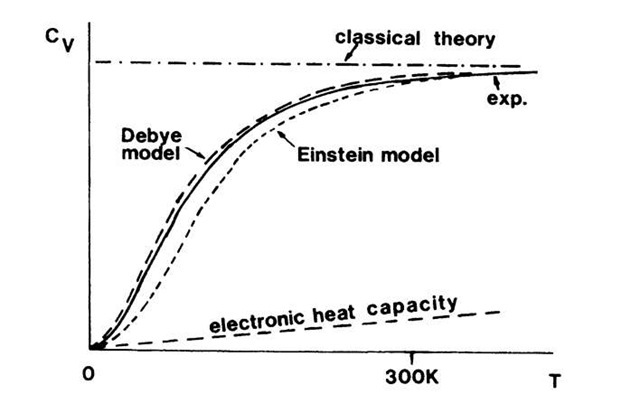
\includegraphics[width=0.8\textwidth]{figures/electronvsphononcv.jpg}
  \caption{La contribución al calor específico de los electrones de
    conducción sólo es relevante a bajas temperaturas, en las que la
    contribución de la red disminuye como $T^3$ y la electrónica de
    manera lineal.}
  \label{fig:electronvsphononcv}
\end{figure}

\section{Dispersión, tiempo libre medio}

Atendiendo a las fuentes de scattering típicas en la red de metales y
aislantes podemos calcular $\kappa$ como
\begin{equation*}
  \kappa = \frac{1}{3} v^2 \tau(T) c_v(T)
\end{equation*}
donde $v^2$ es la velocidad de los portadores del calor (electrones en
metales y fonones en aislantes) y $\tau$ el tiempo medio que los
portadores tienen antes de sufrir una dispersión.

Analizamos la dependencia de $\kappa$ en los extremos del rango de
temperaturas: Muy altas ($T \geq \theta_D$), bajas ($T \sim
\nicefrac{\theta_D}{10}$) y muy bajas ($T \sim 0$).

\subsection*{Temperaturas altas}
\begin{flushright}
  \emph{Aislantes}
\end{flushright}
El principal mecanismo de dispersión de los portadores en los
aislantes son las colisiones con otros fonones, pero sólo los procesos
U son capaces de limitar la conductividad del cristal generando
fonones en dirección contraria al flujo térmico. Deducimos por tanto que el tiempo libre medio está limitado por el número de fonones
disponibles para realizar procesos U:
\begin{equation*}
  \tau \propto \frac{1}{\langle n_q \rangle} = \left[ \frac{1}{1- e^{\beta
      \hbar \omega}} \right]^{-1} \sim \beta \hbar \omega =
\frac{\hbar \omega}{\kb T} \propto T^{-1}
\end{equation*}
Obtenemos, tras utilizar que $c_v \propto \text{cte.}$ (ley de
Dulong-Petit):
\begin{equation*}
  \kappa \propto \tau c_v \propto T^{-1} \cdot \text{cte.} \propto T^{-1}
\end{equation*}
\begin{flushright}
  \emph{Metales}
\end{flushright}
El mecanismo principal de dispersión de los electrones es el
scattering con fonones. El tiempo libre medio estará limitado de igual
forma por el número de fonones:
\begin{equation*}
  \tau \propto \frac{1}{\langle n_q \rangle} = \left[ \frac{1}{1- e^{\beta
      \hbar \omega}} \right]^{-1} \sim \beta \hbar \omega =
\frac{\hbar \omega}{\kb T} \propto T^{-1}
\end{equation*}
Como el calor específico que nos interesa ahora es el electrónico obtenemos
\begin{equation*}
  \kappa \propto \tau c_v \propto T^{-1} \cdot T = \text{cte.}
\end{equation*}

\subsection*{Temperaturas bajas}
\begin{flushright}
  \emph{Aislantes}
\end{flushright}
Los portadores se siguen dispersando principalmente por procesos U.
Para el tiempo libre medio tenemos
\begin{equation*}
  \tau \propto \frac{1}{\langle n_q\rangle} \sim e^{\beta \hbar \omega}
\end{equation*}
Como son procesos U el vector de ondas de los fonones es del tamaño
de la PZB; aproximando $q_{\scriptscriptstyle D} \sim \text{PZB}$
obtenemos $\tau \sim \exp(\theta_D /T)$. Obtenemos, utilizando $c_v
\propto T^3$ (modelo de Debye):
\begin{equation*}
  \kappa \propto \tau c_v \propto e^{\theta_D /T} \cdot T^3
\end{equation*}
Como las temperaturas son muy pequeñas, el término exponencial es más
relevante que el cúbico y $\kappa \sim \exp(\theta_D /T)$
\begin{flushright}
  \emph{Metales}
\end{flushright}
En este caso\footnote{Demostración por criterio de autoridad.} utilizamos el modelo de Debye para modelar el número de fonones $\langle
n_q\rangle$ como $\langle n_q \rangle \propto T^3$. Obtenemos:
\begin{equation*}
  \kappa \propto \tau c_v \propto T^{-3} \cdot T = T^{-2}
\end{equation*}

\subsection*{Temperaturas muy bajas}
\begin{flushright}
  \emph{Aislantes}
\end{flushright}
La principal fuente de scattering de los fonones son fenómenos no
dependientes de la temperatura, como los límites del
cristal. Por ello $\tau \sim \text{cte.}$ y obtenemos
\begin{equation*}
  \kappa \propto \tau c_v \propto \text{cte.} \cdot T^3 \propto T^3
\end{equation*}
\begin{flushright}
  \emph{Metales}
\end{flushright}
De manera similar $\tau$ alcanza un valor constante por las impurezas
de la muestra; la ley de Matthiessen formaliza este resultado.
Obtenemos:
\begin{equation*}
  \kappa \propto \tau c_v \propto \text{cte.} \cdot T \propto T
\end{equation*}







\begin{figure}[h]
  \centering
  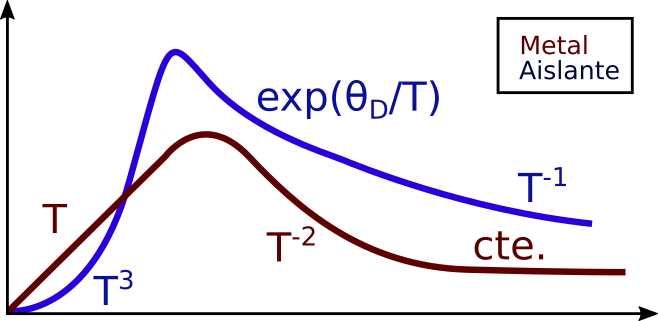
\includegraphics[width=0.8\textwidth]{figures/thermalk.png}
  \caption{Comparativa de la dependencia térmica de la conductividad
    térmica ($\kappa$) para aislantes y metales.}
  \label{fig:thermalk}
\end{figure}

\begin{table}[h]
  \centering
  \begin{tabular}{l|l|l}
  \textbf{Temperatura}&\textbf{Metales}&\textbf{Aislantes}\\ \hline
    Muy baja ($\displaystyle T \sim 0$) &
                                          \begin{tabular}{l}
                                            $\tau_k \propto
                                            \tau_\sigma \sim
                                            \text{cte.}$ 
                                            \\
                                            $c_v \propto T$
                                          \end{tabular}
                                           &
                                          \begin{tabular}{l}
                                            $\tau \sim \text{cte.}$
                                            \\
                                            $ c_v \propto T^3$ 
                                            \\
                                          \end{tabular} \\ \hline
    Baja ($\displaystyle T \sim \nicefrac{\theta_D}{10}$) &
                                          \begin{tabular}{l}
                                            $\tau_k \sim
                                            T^{-3}$ 
                                            \\
                                            $\tau_\sigma \propto
                                            T^{-5}
                                            e^{\theta_{D}/T}$
                                            \\
                                            $c_v \propto T$
                                          \end{tabular}
                                           &
                                          \begin{tabular}{l}
                                            $\tau \sim e^{\theta_D /T}$
                                            \\
                                            $ c_v \propto T^3$ 
                                            \\
                                          \end{tabular} \\ \hline
    Alta ($\displaystyle T \geq \theta_D$) &
                                          \begin{tabular}{l}
                                            $\tau_k \propto
                                            \tau_\sigma \propto T^{-1}
                                            $
                                            \\
                                            $c_v \propto T$
                                          \end{tabular}
                                           &
                                          \begin{tabular}{l}
                                            $\tau \propto T^{-1}$
                                            \\
                                            $ c_v \sim \text{cte.}$
                                            \\
                                          \end{tabular} \\
  \end{tabular}
  \caption{Recordar que $\kappa \propto c_v \tau$ y $\sigma \propto \tau$}
\end{table}

%%% Local Variables:
%%% mode: latex
%%% TeX-master: "../fesi"
%%% End:







\end{document}

%%% Local Variables:
%%% mode: latex
%%% TeX-master: t
%%% End:
